% -*- Mode:TeX -*-

%% IMPORTANT: The official thesis specifications are available at:
%%            http://libraries.mit.edu/archives/thesis-specs/
%%
%%            Please verify your thesis' formatting and copyright
%%            assignment before submission.  If you notice any
%%            discrepancies between these templates and the 
%%            MIT Libraries' specs, please let us know
%%            by e-mailing thesis@mit.edu

%% The documentclass options along with the pagestyle can be used to generate
%% a technical report, a draft copy, or a regular thesis.  You may need to
%% re-specify the pagestyle after you \include  cover.tex.  For more
%% information, see the first few lines of mitthesis.cls. 

%\documentclass[12pt,vi,twoside]{mitthesis}
%%
%%  If you want your thesis copyright to you instead of MIT, use the
%%  ``vi'' option, as above.
%%
\documentclass[11pt,twoside,leftblank]{mitthesis}
%%
%% If you want blank pages before new chapters to be labelled ``This
%% Page Intentionally Left Blank'', use the ``leftblank'' option, as
%% above. 
%\documentclass[11pt,twoside]{mitthesis}
\usepackage{lgrind}
%\usepackage{hyperref}
\usepackage[hidelinks]{hyperref}
\usepackage[table,xcdraw]{xcolor}
\usepackage[usestackEOL]{stackengine}
\usepackage{fixltx2e}
\usepackage{longtable}
%\hypersetup{%hidelinks=true,
%            colorlinks=false,% hyperlinks will be coloured
%            linkcolor=black,% hyperlink text will be green
%            linkbordercolor=white,% hyperlink border will be red
%            citecolor=black, 
%            citebordercolor=white,
%            urlcolor=black
%}
\usepackage{ textcomp }

\usepackage{slantsc}
\usepackage[capitalise,noabbrev]{cleveref}
%\usepackage[capitalise]{cleveref}

\newcommand{\creflastconjunction}{, and\nobreakspace}
\usepackage{titlesec}
\usepackage{lipsum}
\titleformat{\chapter}[display]
  {\normalfont\Large\bfseries\scshape\filcenter}{\chaptertitlename\ \thechapter}{20pt}{\LARGE}
\titlespacing*{\chapter}
  {0pt}{30pt}{20pt}

\titleformat*{\section}{\Large\bfseries}
\titleformat*{\subsection}{\large\bfseries}
\titleformat*{\subsubsection}{\bfseries}

\usepackage{enumitem}
\usepackage{pgfplotstable,filecontents}
\usepackage{multirow}
\usepackage{array}
\usepackage{comment}
\usepackage{ccaption}% http://ctan.org/pkg/ccaption
\usepackage{makecell}
%% These have been added at the request of the MIT Libraries, because
%% some PDF conversions mess up the ligatures.  -LB, 1/22/2014
\usepackage{cmap}
\usepackage[T1]{fontenc}
\pagestyle{plain}
\usepackage[authoryear,round,semicolon]{natbib}
\usepackage{graphicx, pdflscape}
\usepackage[font={small}, labelfont=bf, labelsep=colon]{caption}
%\renewcommand{\thetable}{\arabic{chapter}.\arabic{table}}
%\renewcommand{\thefigure}{\arabic{chapter}.\arabic{figure}}

\newlist{DS2}{enumerate}{1}
\setlist[DS2]{label=Data Sheet 2-\arabic*}
\newlist{DS3}{enumerate}{1}
\setlist[DS3]{label=Data Sheet 3-\arabic*}
\newlist{DS5}{enumerate}{1}
\setlist[DS5]{label=Data Sheet 5-\arabic*}
\pgfplotsset{compat=1.15}

% so we can use rules for table like \toprule
\usepackage{booktabs}

%%% the eg ie and in situ shortcuts
\newcommand{\eg}{\textit{e.g.}\hspace{1mm}}
\newcommand{\ie}{\textit{i.e.}\hspace{1mm}}
\newcommand{\is}{\textit{in situ}\hspace{1mm}}

% so our long table can wrap pages
%\usepackage{longtable}

%\typein [\files]{Enter file names to process, (chap1,chap2 %...), or `all' to
%process all files:}
%\def\all{all}
%\ifx\files\all \typeout{Including all files.} \else %\typeout{Including only \files.} \includeonly{\files} \fi

\begin{document}
\renewcommand{\thetable}{\arabic{chapter}-\arabic{table}}

\title{Movements and oceanographic associations of large pelagic fishes in the North Atlantic Ocean}

\author{Camrin Donald Braun}
\prevdegrees{M.S., King Abdullah University of Science and Technology (2013) \\
B.S., The College of Idaho (2011)}
% If you wish to list your previous degrees on the cover page, use the 
% previous degrees command:
%       \prevdegrees{A.A., Harvard University (1985)}
% You can use the \\ command to list multiple previous degrees
%       \prevdegrees{B.S., University of California (1978) \\
%                    S.M., Massachusetts Institute of Technology (1981)}
\department{Joint Program in Applied Ocean Science \& Engineering\\Massachusetts Institute of Technology\\ \& Woods Hole Oceanographic Institution}

% If the thesis is for two degrees simultaneously, list them both
% separated by \and like this:
% \degree{Doctor of Philosophy \and Master of Science}
\degree{Doctor of Philosophy}

% As of the 2007-08 academic year, valid degree months are September, 
% February, or June.  The default is June.
\degreemonth{September}
\degreeyear{2018}
\thesisdate{August 10, 2018}

%% By default, the thesis will be copyrighted to MIT.  If you need to copyright
%% the thesis to yourself, just specify the `vi' documentclass option.  If for
%% some reason you want to exactly specify the copyright notice text, you can
%% use the \copyrightnoticetext command.  
%\copyrightnoticetext{\copyright IBM, 1990.  Do not open till Xmas.}

\copyrightnoticetext{\copyright 2018 Camrin Donald Braun. All rights reserved.  
\\ The author hereby grants to MIT and WHOI permission to reproduce and 
to distribute publicly paper and electronic copies of this thesis document 
in whole or in part in any medium now known or hereafter created.}

% If there is more than one supervisor, use the \supervisor command
% once for each.
\supervisor{Simon R. Thorrold}{Senior Scientist\\Woods Hole Oceanographic Institution}

% This is the department committee chairman, not the thesis committee
% chairman.  You should replace this with your Department's Committee
% Chairman.
\chairman{Ann Tarrant}{Chair, Joint Committee for Biological Oceanography\\Massachusetts Institute of Technology\\Woods Hole Oceanographic Institution}

% Make the titlepage based on the above information.  If you need
% something special and can't use the standard form, you can specify
% the exact text of the titlepage yourself.  Put it in a titlepage
% environment and leave blank lines where you want vertical space.
% The spaces will be adjusted to fill the entire page.  The dotted
% lines for the signatures are made with the \signature command.
\maketitle

% The abstractpage environment sets up everything on the page except
% the text itself.  The title and other header material are put at the
% top of the page, and the supervisors are listed at the bottom.  A
% new page is begun both before and after.  Of course, an abstract may
% be more than one page itself.  If you need more control over the
% format of the page, you can use the abstract environment, which puts
% the word "Abstract" at the beginning and single spaces its text.

%% You can either \input (*not* \include) your abstract file, or you can put
%% the text of the abstract directly between the \begin{abstractpage} and
%% \end{abstractpage} commands.

% First copy: start a new page, and save the page number.
\cleardoublepage
% Uncomment the next line if you do NOT want a page number on your
% abstract and acknowledgments pages.
% \pagestyle{empty}
\setcounter{savepage}{\thepage}
\begin{abstractpage}
% $Log: abstract.tex,v $
% Revision 1.1  93/05/14  14:56:25  starflt
% Initial revision
% 
% Revision 1.1  90/05/04  10:41:01  lwvanels
% Initial revision
% 
%
%% The text of your abstract and nothing else (other than comments) goes here.
%% It will be single-spaced and the rest of the text that is supposed to go on
%% the abstract page will be generated by the abstract page environment.  This
%% file should be \input (not \include 'd) from cover.tex.
 Marine phytoplankton are central players in the global carbon cycle, responsible for nearly half of global primary production. The identification of the major factors controlling phytoplankton ecology, physiology, and, ultimately, bloom dynamics has been a central problem in the field of biological oceanography for the past century. From physical explanations (Sverdrup's critical depth hypothesis), to chemical rational (Redfield ratio), to ecological theory (Margalef's mandala), the field has been constantly reevaluating evidence to answer the question: What drives phytoplankton blooms? Molecular approaches enable the direct examination of species-specific metabolic profiles in mixed, natural communities, a task which was previously intractable. In this thesis, I developed and applied novel analytical tools and bioinformatic pipelines to characterize the physiological response of phytoplankton at various levels of taxonomic grouping (strain, species, and functional group) to their environment.   \par
An in silico Bayesian statistical approach was designed to identify stable reference genes from high-throughput sequence data for use in RT-qPCR assays or metatranscriptome studies. Using this approach, the first field study, focusing on the species-level, was designed to examine the role of resource partitioning in the coexistence of two closely related diatom species in the same estuarine system. This study demonstrated that co-occurring diatoms in a dynamic coastal marine system have apparent differences in their capacity to use nitrogen and phosphorus, and that these differences may facilitate the diversity of the phytoplankton. The second field study focused on the diatom, haptophyte, and dinoflagellate functional groups and used simulated blooms to characterize the traits that govern the magnitude and timing of phytoplankton blooms in the oligotrophic ocean. The results indicated that blooms form when phytoplankton are released from limitation by resources (nutrients, vitamins, and trace metals) and that the mechanistic basis for the success of one functional group over another may be driven by how efficiently the transcriptome is modulated following a nutrient pulse. The final study looked at the sub-species level, examining the balance of phenotypic plasticity and strain diversity in the success of the cosmopolitan coccolithophore \textit{Emiliania huxleyi}. These data suggest that following perturbation there was a shift in strain composition as well as significant changes in transcript abundance of key biogeochemical genes involved in nutrient acquisition, calcification, and the life stage of the population.\par
Together, these studies demonstrate the breadth of information that can be garnered through the integration of molecular approaches with traditional biological oceanographic surveys, with each illuminating fundamental questions around phytoplankton ecology and bloom formation.




\end{abstractpage}

% Additional copy: start a new page, and reset the page number.  This way,
% the second copy of the abstract is not counted as separate pages.
% Uncomment the next 6 lines if you need two copies of the abstract
% page.
% \setcounter{page}{\thesavepage}
% \begin{abstractpage}
% % $Log: abstract.tex,v $
% Revision 1.1  93/05/14  14:56:25  starflt
% Initial revision
% 
% Revision 1.1  90/05/04  10:41:01  lwvanels
% Initial revision
% 
%
%% The text of your abstract and nothing else (other than comments) goes here.
%% It will be single-spaced and the rest of the text that is supposed to go on
%% the abstract page will be generated by the abstract page environment.  This
%% file should be \input (not \include 'd) from cover.tex.
 Marine phytoplankton are central players in the global carbon cycle, responsible for nearly half of global primary production. The identification of the major factors controlling phytoplankton ecology, physiology, and, ultimately, bloom dynamics has been a central problem in the field of biological oceanography for the past century. From physical explanations (Sverdrup's critical depth hypothesis), to chemical rational (Redfield ratio), to ecological theory (Margalef's mandala), the field has been constantly reevaluating evidence to answer the question: What drives phytoplankton blooms? Molecular approaches enable the direct examination of species-specific metabolic profiles in mixed, natural communities, a task which was previously intractable. In this thesis, I developed and applied novel analytical tools and bioinformatic pipelines to characterize the physiological response of phytoplankton at various levels of taxonomic grouping (strain, species, and functional group) to their environment.   \par
An in silico Bayesian statistical approach was designed to identify stable reference genes from high-throughput sequence data for use in RT-qPCR assays or metatranscriptome studies. Using this approach, the first field study, focusing on the species-level, was designed to examine the role of resource partitioning in the coexistence of two closely related diatom species in the same estuarine system. This study demonstrated that co-occurring diatoms in a dynamic coastal marine system have apparent differences in their capacity to use nitrogen and phosphorus, and that these differences may facilitate the diversity of the phytoplankton. The second field study focused on the diatom, haptophyte, and dinoflagellate functional groups and used simulated blooms to characterize the traits that govern the magnitude and timing of phytoplankton blooms in the oligotrophic ocean. The results indicated that blooms form when phytoplankton are released from limitation by resources (nutrients, vitamins, and trace metals) and that the mechanistic basis for the success of one functional group over another may be driven by how efficiently the transcriptome is modulated following a nutrient pulse. The final study looked at the sub-species level, examining the balance of phenotypic plasticity and strain diversity in the success of the cosmopolitan coccolithophore \textit{Emiliania huxleyi}. These data suggest that following perturbation there was a shift in strain composition as well as significant changes in transcript abundance of key biogeochemical genes involved in nutrient acquisition, calcification, and the life stage of the population.\par
Together, these studies demonstrate the breadth of information that can be garnered through the integration of molecular approaches with traditional biological oceanographic surveys, with each illuminating fundamental questions around phytoplankton ecology and bloom formation.




% \end{abstractpage}

\cleardoublepage
\null\vfill
{\raggedleft\vfill\itshape\Longstack[l]{
  For ...short sweet dedication here. kitty?\bigskip\bigskip\space}\par
}
\cleardoublepage

\section*{\centerline{\LARGE\textsc{Acknowledgments}}}

{\parindent15pt

\singlespace
During my time in the MIT-WHOI Joint Program, I have been supported by the NASA Earth and Space Science Fellowship, the MIT John S. Hennessy Fellowship, the MIT Martin Family Society of Fellows for Sustainability Fellowship, the WHOI Ocean Venture, Grassle, and James Stratton Fellowships and the WHOI Academic Programs Office. This research and its dissemination was supported by funds from National Geographic, Amazon Web Services, the Explorers Club, Rolex, Sigma Xi, the MIT Center for International Studies, WHOI Access to the Sea and Coastal Ocean Institute Funds, MIT Graduate Student Council, MIT Student Assistance Fund, WHOI Biology Department, the American Fisheries Society, the WHOI Academic Programs Office and many individual donors. For all of your support, large and small, I am eternally grateful. \par\bigskip

This thesis is a product of a significant amount of time spent on boats. I especially thank Willy Hatch and the M/V Machaca, fishermen in the Shark's Eye Tournament in Montauk, New York, Chris Fischer and the M/V OCEARCH, Eric Savetsky, Tom Burns and the M/V Endurance, the R/V Pelican and the many other men, women and vessels for assistance in field tagging operations. Without your tireless support, this work would not have been possible.

SIMON

I am grateful to my thesis committee, Glenn Flierl, Gareth Lawson, Dennis McGillicuddy and Greg Skomal, for graciously contributing their time to this endeavor and for their valuable feedback along the way. I would also like to thank my co-authors: Peter Gaube, Ben Galuardi, Greg Skomal, Pedro Afonso, Jorge Fontes and Tane Sinclair-Taylor. C.H. Lam contributed code to several pieces of my work.

To the many amazing people in my life during my time as a student, an enormous thank you for your support and the memories we shared. Lobster fishing in blizzards, diving remote tropical atolls and our many other adventures will stick with me forever.

I am especially grateful for the support from my family who instilled in me a love for being outside, taught me that curiosity in fact did not kill the cat and for sticking with me despite my love affair with a rather fiscally-irresponsible career.


}
 





\pagestyle{plain}
  % -*- Mode:TeX -*-
%% This file simply contains the commands that actually generate the table of
%% contents and lists of figures and tables.  You can omit any or all of
%% these files by simply taking out the appropriate command.  For more
%% information on these files, see appendix C.3.3 of the LaTeX manual. 
\tableofcontents
\newpage
\listoffigures
\newpage
\listoftables



\chapter{Introduction}
\raggedbottom
\clearpage


\section{Background}
%initial hypotheses about where animals go and driving question(s)
Marine ecology, particularly of the open ocean, is the study of marine organisms in the context of each other and the environment. The open ocean is characterized by a range of temporal and spatial scales that are manifested as a complex integration of physical, chemical and biological phenoma. Ocean physics and biology interact to generate the behaviors we observe, yet animal movements are typically observed at basin scales, revealing fascinating long-distance migrations, or at very small scales when, for example, they interact with fishing effort. Scales below thousands of kilometers and months are poorly understood. However, perhaps the most important biophysical interactions occur at and below the oceanic mesoscale. This lack of knowledge stems from issues inherent in studying animal movements in an opaque medium, particularly with constraints on geolocation of individual fish as they move around. 

Since the first tag-recapture experiments on Atlantic salmon in 1873 \citep{Everhart1975}, scientists have been actively studying animal movements. Where animals go and what they do there is of fundamental importance for everything from ocean properties, such as carbon export \citep{Lavery2010a}, to ecosystem structure \citep{Thorrold2014} and fishery dynamics \citep{Block2005}. Yet, despite significant technological advances in tag technology, we remain constrained by studying animals that move thousands of kilometers while diving from the surface to bathypelagic (> 2000 m) all while immersed in an opaque medium that is seawater. Our current understanding of large pelagic fish behavior is largely limited to large-scale movements and behavior summaries derived from light-level geolocation by archival tags. The accuracy of light geolocation ($\pm$100-200 km; ~10,000 km\textsuperscript{2}) and its depth limits (< 100 m) constrain its application to large-scale surface movements. Yet, many fishes exhibit diving behavior that renders light geolocation impossible, and the magnitude of error precludes our ability to resolve important ecological dynamics such as habitat association (\eg specific bathymetric or oceanographic feature use). Therefore, improved analytical techniques and different approaches to tracking studies are necessary to acquire more accurate position information with which we can characterize the ocean environment and provide the context for the animal behaviors we observe.

Thus, I focus on the following questions in this thesis:

%enumerate questions
\begin{enumerate}
    \item How can we improve existing methods of geolocation within the constraints of existing archival tag technology?
    \item Can we use improved methods to leverage historical data for use in modern physical-biological interaction studies, and, by doing so, improve the inference we can gain from this data?
    \item How can we apply the lessons learned from the first two questions to design a study that alleviates the limitations inherent in these approaches such that we can quantify use of specific oceanographic features?
\end{enumerate}

\subsection{It's a big ocean and approaches to locating animals}
% animal movement in general and why its historically been difficult to follow things in the ocean
The study of animal movements in the ocean remains a formidable challenge due to the difficulty of making observations in an opaque medium, only a fraction of which can we directly observe. As such, we understand relatively little about the ecology of marine fishes compared to terrestrial taxa. Information on large pelagic fishes that occur in the open ocean is particularly lacking, despite lucrative fisheries and intense fishing effort for a number of these species. Basin-scale movements \citep{Skomal2009} and deep forays into the meso- and bathypelagic layers of the open ocean \citep{Thorrold2014a} further complicate this research by making individuals even less available for direct observations than coastal fish species.

Historically, insights into pelagic fish ecology were limited to those obtained visually and at the surface. These constraints allowed access to only a small portion of any species' lifetime movements and behavior, and it has long been recognized that novel approaches are needed to better understand the ecology of these fishes. Mark-recapture techniques employing external tags have been used extensively since the early twentieth century, but this approach only provides deployment and retrieval locations with no data on a fish's behavior in the interim \citep{Kohler2001}.

The development of electronic tags in the mid-1950s has since enabled researchers to gather a more holistic view of the behaviors of large pelagic organisms. Temperature and pressure sensors developed simultaneously in the 1970s and transformed our ability to follow the incredible dives that many species perform \citep{Carey1981}. Satellite transmitting tags followed in the 80s and allowed accurate positioning of surface-oriented species such as basking sharks \citep{Priede1984}. Data storage, or archival, tags were first deployed in the 1990s, effectively spurring an increasing global trend in the number of satellite tag studies since \citep{Hussey2015}. Modern tags incorporate multiple sensors (including acoustics, accelerometers and cameras) and can release themselves from a study animal, effectively eliminating the fishery-dependent nature of earlier studies. While other tracking technologies exist, the two most widely used methods in aquatic ecosystems today are acoustic and satellite telemetry \citep{Hussey2015}.

Acoustic techniques proliferated starting in the 1960s and have since made many significant contributions to the field \citep[\eg][]{Carey1981, Carey1990}. These techniques rely on transmission of acoustic signals by tagged animals that are logged at moored or mobile receiving stations. Acoustic studies now boast tags that last up to 10 years, typically exhibit error on the order of meters and, in some cases, can leverage satellite-linked loggers that eliminate the need to recover devices to access stored data \citep{Donaldson2014}. The benefits of acoustic telemetry have driven exceptional growth in acoustic monitoring studies \citep{Hussey2015}; however, current acoustic studies are limited to < 2 km range from receiving stations (\eg hydrophones) which proves intractable for studying highly migratory species in the open ocean. Thus, the major limitation with this approach is scale which is perhaps among the most interesting ocean challenges \citep{Stommel1963, Haury1978}. 

In the late 1980s, satellite-linked archival tags followed the advent of acoustic devices. This technology alleviated the infrastructure, and thus scaling, issues associated with acoustic telemetry, enabling researchers to follow fish that move thousands of kilometers across ocean basins in a matter of months, such as tunas (block tuna paper) and pelagic sharks (ref). Since their inception, these tags have become increasingly relevant \citep{Hussey2015} for studying horizontal and vertical movements \citep{Block2011, Thorrold2014a, Berumen2014}, residency \citep{Domeier2006}, mortality \citep{Musyl2011a}, aggregative and feeding behaviors \citep{Jorgensen2012}, and other aspects of the biology and ecology of marine organisms. Pop-up satellite archival transmitting (PSAT) tags, specifically, have been used with great success on a number of taxa \citep{Hussey2015}. These devices are attached externally to a study animal and are programmed to pop-up from the animal after a predetermined deployment period. While active on the animal, these tags typically collect an \is time series of depth, temperature and light levels. Miniaturization and ever-improving sensors, batteries and storage capabilities make this a rapidly advancing field that has already demonstrated vast improvements over previous techniques. As such, this technology has been deployed on thousands of study animals encompassing nearly all marine taxa large enough to carry a tag \citep{Hussey2015}. These studies have now consequently described the broad-scale horizontal and vertical movements for many marine species. However, fewer studies attempt to perform quantitative analyis of how species interact with and choose to occupy the surrounding oceanographic environment \citep[except see, for example, ][]{Lawson2010}.

\subsection{I tagged some fish, now what}\label{sec:geo}
% analytical approaches to tag data and geolocation
Despite all these advances, we remain limited by the fundamental physics of transmitting electromagnetic radiation (the way we communicate with satellites such as GPS) through an opaque medium such as seawater. As such, even cutting edge satellite technologies for fish still archive light data for geolocation. Ambient light records are used to estimate dawn and dusk from which longitude (local noon) and latitude (local day length) are derived to estimate positions \citep{Hill1994, Hill2001}. The community recognized the need to supplement light-based geolocation with other information early on, and we have since made sizeable advances in analytic approaches to improved geolocation despite the age-old constraints. 

% Here's a synopsis of what people have done...hill, sibert, lam, nielsen, pedersen, thygesen, etc
Arguably the most important advances in the analysis of animal movement data, including the geolocation problem, has been state-space models which estimate the "state" of an unobserved process from an observed dataset \citep{Jonsen2013}. 
Perhaps the most notable early advance was the Kalman filter (that has applications from natural sciences to economics) by \cite{Sibert2001} being used to analyze position estimates from noisy light data \citep{Hill2001}. Further advances were quickly achieved by incorporating a comparison of \is SST recorded by the tag and remotely-sensed measures \citep{Teo2004, Nielsen2006}. Improvements since have expanded rapidly to incorporate other ancillary data such as tidal variation \citep[\eg][]{Metcalfe1997} to inform geolocation and more sophisticated modelling techniques such as hidden Markov models \citep[\eg][]{Pedersen2008}. By coupling the integration of \is measurements onboard archival tags with ever-improving statistical techniques and modern tools such as high-resolution oceanographic models and a suite of remote-sensing satellites, we are realizing significant improvements in estimating animal movements over geolocation with light levels alone.

\subsection{Biophysical interactions in the ocean}
% biophysical interactions in the ocean & drivers of animal movements


% start with general dynamics and structuring of ocean ecosystems
Of particular interest relevance for this thesis is the role that oceanography plays in the structuring of pelagic ecosystems. Fronts and mesoscale eddies are among the most important features in the open ocean \citep{Chelton2011, McGillicuddy2016, Mahadevan2016}, and recent advances in satellite oceanography have allowed the automated identification and tracking of these features globally \citep{Chelton2011, Belkin2009}. These advances in our ability to observe and track these features have revealed rich regional variability in how these features influence lower trophic levels \citep{McGillicuddy2016, Gaube2017DSR} and have shown the potential coupling of biology and ocean physics that can lead to the formation of biological hotspots \citep{Mann2006, Belkin2014}.

%and have most recently led to studies of how these features might influence animal populations \citep[\eg][]{Kobayashi2011, Gaube2017, Belkin2014, Queiroz2016}.

% very brief what we know about non-fish
Electronic tag technologies permit quantitative analyses of the use of these features by pelagic predators. Due to geolocation constraints (see Section \ref{sec:geo}), the vast majority of advances have been made on obligate surface-oriented taxa such as turtles \citep[\eg][]{Gaube2017, Polovina2006, Kobayashi2011}, marine mammals \citep[\eg][]{Johnston2007, Bailleul2010} and birds \citep[\eg][]{Thorne2013, TewKai2009}. Together, these studies suggest the most important features for pelagic predators are likely to be associated with enhanced vertical flux of nutrients leading to increases in primary production \citep{Franks1992}. Convergent flow at front boundaries and along the periphery of eddies can also aggregate passive particles, including phytoplankton, and these areas are thought to attract pelagic predators due to increased foraging opportunities, generating hotspots \citep{Scales2014}.

% history of biophysical interactions for fishes, focus on HMS. demonstrate how this is traditionally done w/ catch data which is inherently flawed. incorporate, for example, hobday & hartog

Historically, anecdotal evidence and fisheries statistics have supported the association of pelagic fishes with physical structures like fronts and eddies \citep[e.g.,][]{Hobday2014}, but scientists currently understand very little about the biology of these important oceanographic features, particularly for fish communities. Technological limitations inherent in light-level geolocation \citep{Braun2015} have largely precluded robust analyses of the associations between (sub)mesoscale oceanographic structures and pelagic fishes. Conventional light-level geolocation from analysis of archival tag data is generally insufficiently accurate to match fish movements with specific mesoscale features detected from satellite observations. As a result, we understand little about the biophysical factors influencing the ecology of large pelagic fishes. Despite these constraints, some progress has been made, primarily using fisheries data. For example, \cite{Hsu2015} compared catch data from the U.S. northwest Atlantic longline fishery to the mesoscale eddy field in this region and found bluefin tuna associated with anticyclonic mesoscale eddies while swordfish were more often outside of eddies. Similarly, using catch data, \cite{Hobday2014} found southern bluefin tuna associated with anticyclones off Australia while opah preferred cyclonic eddies. Similar analyses have been conducted using other fisheries, species and ocean features, such as fronts \citep[\eg][]{Worm2005}.

A few recent studies have used tracking data to investigate overlap between pelagic fishes and ocean features. For example, \cite{Miller2015} showed basking sharks prefer productive regions of the Northeast Atlantic characterized by contemporaneous thermal and chlorophyll fronts. And \cite{Gaube2018} showed two tagged white sharks associated with anticyclonic eddies of the Northwest Atlantic, suggesting these features may influence foraging opportunities. However, analyzing fisheries-independent tracking data in the context of (sub)mesoscale oceanography remains an anomalous approach due largely to geolocation issues mentioned above. In addition, few studies of fish movements have been specifically designed to investigate feature use. Thus, linking movements of pelagic fishes with (sub)mesoscale physical-biological mechanisms remains largely unstudied but is critical to understanding the structuring of pelagic ecosystems and to designing appropriate management approaches for pelagic fish populations.

\subsection{Practical considerations and applications}
 % primarily to fisheries management problems
 
 Over the past century, human exploitation of natural systems has propagated throughout the ocean, subjecting large marine predators to intense exploitation \citep{Byrne2017} and eliciting disproportionate effects on large vertebrates \citep{Jackson2001, Baum2003}. As a result of intense anthropogenic impact, many predatory fish populations (including billfish, tuna and sharks) have joined the ranks of immediate conservation concern, and their populations are routinely depleted by 50-70\% \citep{Hilborn2003} and up to 90\% \citep{Myers2005}. Many of these species spend most of their life in the open ocean and traverse vast expanses of water in search of food, reproductive opportunities and suitable habitat. Their behavioral tendencies subject them to fishing pressure by an array of different gear types and exploitation levels under different national jurisdictions and throughout the high seas. In addition, the current lack of information about key life history traits, population size, movements and habitat use of these fishes amplifies the problem of managing these populations as anthropogenic pressures on fishes continue to rise \citep{Dulvy2008, Ferretti2010}.

A central challenge to the management of ocean seascapes is the dynamic spatial and temporal nature of ocean systems \citep{Lewison2015}. Yet, traditional ocean management approaches are most often static. Static management approaches may be less effective for managing highly migratory species and are less able to respond to changing ocean dynamics from ephemeral features to chronic changes in our climate and ocean. Relatively simple time series of animal movements and behavior coupled with modeled and/or remotely-sensed representations of the marine environment, as described in this thesis, can be combined to develop tools for near real-time prediction of animal movement based and species-specific habitat use. These dynamic approaches will be critical for managing fisheries in a changing ocean \citep{Maxwell2015}, but necessitate some understanding of physical-biological mechanisms governing the observed animal behaviors.

Filling these gaps will be essential for formulating effective management plans \citep{Cullis-Suzuki2010}, understanding the potential effects of climate change \citep{Hazen2012} and ensuring continued harvest of these resources \citep{Pauly1998, Watson2013}. Additionally, an improved understanding of the behaviors of large pelagic fishes will not only inform us about the ecology of the taxa themselves, but may also facilitate broader understanding of biogeochemical processes in the ocean \citep{Lavery2010, Roman2010}.

\section{Thesis Overview}
% overarching goal
%This thesis quantifies the movement and oceanographic association of pelagic fishes.

% chapter-specific list-like paragraph
In chapter \cref{chap:2}, I developed significant methodological improvements for geolocating fishes equipped with traditional archival tags. Blue and mako sharks were instrumented both with PSATs and an independent Doppler-based satellite tag from which "known" locations were used to quantify error in the resulting PSAT geolocation model. Leveraging three-dimensional data from tags in conjunction with high-resolution oceanographic models facilitated significant improvements in error estimates relative to existing model frameworks. In chapters \cref{chap:3} and \cref{chap:4}, I applied this modeling technique to basking shark and swordfish datasets, respectively. These two species have proven particularly difficult to track due to significant occupation of the aphotic regions of the ocean resulting in little to no light data available for geolocation. In \cref{chap:3} I used the more accurate locations to quantify large-scale movements, seasonality and vertical habitat use of > 50 basking sharks in the western Atlantic. Improved swordfish tracks in \cref{chap:4} were also used to investigate movements and seasonality and, in some cases, were accurate enough to describe mesoscale feature use. I also mined fisheries-dependent data for swordfish in the North Atlantic in \cref{chap:4} that I synthesized with fishery-independent electronic data to quantify oceanographic influences on swordfish. Finally, \cref{chap:5} focused on building a robust dataset with which I could test interactions between pelagic predators and mesoscale eddies. I double-tagged 15 blue sharks (as above) in order to reconstruct 3-D movements in the Gulf Stream eddy field and collocated these data to remotely-sensed and modeled oceanographic data to quantify shark-eddy interactions. Overall, I demonstrate that integrating observations of animal movement and behavior with satellite imagery and physical data provides significantly enhanced insight on habitat preferences and the interactions of an animal with its environment, a critical dataset for disentangling natural trends from those associated with the impacts of human activities such as fishing pressure in a changing ocean.

%--------------------------------
\begin{comment}


drawing conclusions about the function of diving (block electronic tagging book) and oceanographic associations since the first quality datasets from electronic tags in the 1990s

bakun around p. 6 for discussion of "scales" and pattern

% ** see good reviews such as hobday and hartog or mcgillicuddy ann rev mar sci **

As a result, we understand little about the biophysical factors influencing the ecology of large pelagic fishes.


%Mesoscale eddies and submesoscale fronts make up the internal weather of the ocean, exciting vertical fluxes and transporting pelagic communities hundreds to thousands of kilometers. Yet, while the application of satellite technology now allows us to view these features in almost real time, the influence of these structures on pelagic predators remains largely unknown. With the latest satellite tagging technologies, we now have the ability to observe the movement of large oceanic predators in high-resolution, three-dimensional space. Here, we propose to investigate the use of mesoscale eddies and meanders and submesoscale fronts by pelagic predators in the North Atlantic by collocating trajectories obtained from satellite-tagged sharks with (sub)mesoscale structures, defined here as features with spatial scales of $O(1 - 100\ km)$, identified and tracked in maps of sea level anomalies and sea surface temperature. The collocation of individual sharks, as model apex predators, with (sub)mesoscale ocean features will allow us to understand how these predators use these ubiquitous structures. Furthermore, by comparing observed patterns of feature use by the predators to satellite observations of ocean currents, surface temperature, and ocean color, I link observed behavior to known (sub)mesoscale physical/biological processes. Thus, the goal of the research proposed here is to determine the influence of (sub)mesoscale oceanographic features on the movements of pelagic predators, allowing us to link predator behavior to (sub)mesoscale physical/biological mechanisms, through the synergistic analysis of individual fish movement and concurrent satellite observations of (sub)mesoscale eddies, meanders and fronts.

% Of particular interest to this study is the role that (sub)mesoscale oceanography plays in the structuring of pelagic ecosystems and the movement ecology of large pelagic fishes. Historically, anecdotal evidence and fisheries statistics have supported the association of pelagic fishes with mesoscale structures like fronts and eddies \citep[e.g.,][]{hobday2014derived}, but scientists currently understand very little about the biology of these important oceanographic features. Furthermore, little data is available on fish communities that inhabit these structures. Electronic tag technologies now permit quantitative, fisheries-independent analyses of the use of these features by pelagic predators. Recent work has shown that obligate surface-dwelling marine organisms (e.g. turtles, seals, and birds) associate with persistent mesoscale fronts (reviewed in \cite{scales2014review}), and limited research on fishes has shown the importance of seasonally persistent fronts for basking sharks \citep{miller2015}. Technological limitations inherent in light-level geolocation \citep{braun2015movements} have, however, largely precluded robust analyses of the associations between (sub)mesoscale oceanographic structures and pelagic fishes. Conventional light-level geolocation from analysis of archival tag data is generally insufficiently accurate to match fish movements with specific mesoscale features detected from satellite observations. However, fin-mounted tags capable of generating positions by interrogating ARGOS satellites provide sufficiently accurate positions for (sub)mesoscale collocation analyses. In addition, this technology can be paired with conventional PSAT tags that provide detailed information on the vertical movements and water column properties. Together, the tags can provide high-resolution $(\sim 60\ sec)$ measurements of vertical movements with a spatial accuracy appropriate for matching resulting tracks to concurrent (sub)mesoscale oceanographic structures.




which involved integrating SST...that achieved so much ...numbers...improvement over light alone.



However, by integrating additional \is measurements onboard archival tags ...

can now get geolocation down below theoretical light thresholds using modern tools such as high-resolution oceanographic models and a suite of remote-sensing satellites. in combination, we're now better able than ever before to contextualize the observations we make using tagged animals that can teach us both about the animals and about the ocean.


The issue of scale is described by \cite{Haury1978} as the "great variability...on all scales in space and time caused by patchiness." This refers to the nested nature of ocean phenomena and the complexity in interpreting an observation in...by itself...


that are intimately tied to 

Physical-biological interactions that drive the behaviors we observe.

physical mechanisms

Processes observed in the open ocean are an integration of physical, chemical and biological phenomena that

The ocean is a complex medium, characterized by a range of scales
the issue of scale in the ocean

AND

animal movements at basin-scale and long time periods, relatively well understood and revealed fascinating migrations. enter history stuff like original basker paper and carey's work

BUT

scales below hundreds/thousands of kms and months are poorly understood. yet, this is where the interesting stuff happens. this stems from issues with opaque medium and geolocation.

THEREFORE

due to tech and methodological improvements, i can probably do better. In this thesis, i seek to:

Improvements in satellite tag technology and advances in analytical techniques would facilitate acquisition of better position information with which we could contextualize animal behaviors in their environment. 





\subsection{Aquatic telemetry}
% progress to date but what remains to be done. bit of history is good here

% animal movement in general and why its historically been difficult to follow things in the ocean
The study of animal movements in the ocean remains a formidable challenge due to the difficulty of making observations in an opaque medium, only a fraction of which can we directly observe. We understand relatively little about the ecology of marine fishes when compared to terrestrial taxa. Information on large pelagic fishes that occur in the open ocean is particularly lacking, despite lucrative fisheries and intense fishing effort for a number of these species. Basin-scale movements \citep{Skomal2009} and deep forays into the meso- and bathypelagic layers of the open ocean \citep{Thorrold2014a} further complicate this research by making individuals even less available for direct observations than coastal fish species. As a result, we understand little about the biophysical factors influencing the ecology of large pelagic fishes.

% aquatic telemetry, focus on sat telemetry
Historically, insights into pelagic fish ecology were limited to those obtained visually and at the surface. These constraints allowed access to only a small portion of any species' lifetime movements and behavior, and it has long been recognized that novel approaches are needed to better understand the ecology of these fishes. Mark-recapture techniques employing external tags have been used extensively sincet he early twentieth century, but this approach only provides deployment and retrieval locations iwth no data on a fish's behavior in the interim \citep{Kohler2001}.

The development of electronic tags has enabled researchers to gather a more holistic view of the behaviors of large pelagic organisms. Acoustic techniques proliferated starting in the 1960s and have since made many significant contributions to the field \citep[\eg][]{Carey1981}. Satellite-linked archival tags followed in the late 1980s and have enabled further important advances. Since their inception, these tags have become increasingly relevant \citep{Hussey2015} for studying horizontal and vertical movements \citep{Block2011, Thorrold2014a, Berumen2014}, residency \citep{Domeier2006}, mortality \citep{Musyl2011a}, aggregative and feeding behaviors \citep{Jorgensen2012}, and other aspects of the biology and ecology of marine organisms.

Pop-up satellite archival transmitting (PSAT) tags, specifically, have been used with great success on a number of taxa \citep{Hussey2015}. These devices are attached externally to a study animal and are programmed to pop-up from the animal after a predetermined deployment period. While active on the animal, these tags typically collect an \is time series of depth, temperature and light levels. Miniaturization and ever-improving sensors, batteries and storage capabilities make this a rapidly advancing field that has already demonstrated vast improvements over previous techniques. As such, this technology has been deployed on thousands of study animals encompassing nearly all marine taxa large enough to carry a tag \citep{Hussey2015}. These studies have now consequently described the broad-scale horizontal and vertical movements for many marine species. However, fewer studies attempt to perform quantitative analyis of how species interact with and choose to occupy the surrounding oceanographic environment \citep[except see, for example, ][]{Lawson2010}.


\subsection{Pelagic fish ecology}
% importance of these species. why care about HMS? finish with large-scale looming question
% impressive movements (horiz and vert). commercially relevant.


\subsection{Practical considerations}
Over the past century, human exploitation of natural systems has propagated throughout the ocean, subjecting large marine predators to intense exploitation \citep{Byrne2017} and eliciting disproportionate effects on large vertebrates \citep{Jackson2001, Baum2003}. As a result of intense anthropogenic impact, many predatory fish populations, including billfish, tuna and sharks, have joined the ranks of immediate conservation concern, and their populations are routinely depleted by 50-70\% \citep{Hilborn2003} and up to 90\% \citep{Myers2005}. Many of these species spend most of their life in the open ocean and traverse vast expanses of water in search of food, reproductive opportunities and suitable habitat. Their behavioral tendencies subject them to fishing pressure by an array of different gear types and exploitation levels under different national jurisdictions and throughout the high seas. In addition, the current lack of information about key life history traits, population size, movements and habitat use of these fishes amplifies the problem of managing these populations as anthropogenic pressures on fishes continue to rise \citep{Dulvy2008, Ferretti2010}.

dynamic ocean management

Relatively simple time series of continuous geolocation data and information on individual diving and ambient temperature from satellite tags can facilitate robust analyses and interpretation of individual movements. These data, in combinatoin with auxiliary enviornmental data and advanced analysis techniques, provide a unique opportunity to answer many unresolved questions regarding behavior and ecology of large pelagic fishes. Filling these gaps will be essential for formulating effective management plans \citep{Cullis-Suzuki2010}, understanding the potential effects of climate change \citep{Hazen2012} and ensuring continued harvest of these resources \citep{pauly1998, Watson2013}. Additionally, an improved understanding of the behaviors of large pelagic fishes will not only inform us about the ecology of the taxa themselves, but may also facilitate broader understanding of biogeochemical processes in the ocean \citep{Lavery2010, Roman2010}.

Part of the paucity of information governing our understanding of deep-water occupation by large pelagic fishes is due to the analytical limitations associated with PSAT tag data. While they provide high-resolution information on vertical behaviors, accurate horizontal positions require frequent surface occupation. This presents a significant constraint on studying marine species, many of which leave the surface for months at a time \citep{Skomal2009}.




% what this technique has taught us about movements of fish.
    % while impressive movements (horiz and vert), lot of work to be done to, for example, undertsand mechanisms driving movements.

% the single most important barrier to this has been error in fihs geolocation. here's why this is an issue.

% brings us to the questions? 
    % 1) how to better geolocate animals using oceanographic data? 
    % 2) oceanographic influences on animal movements? biophysical interactions?
    % 3) dynamic oceanography drive biology, the formation and degradation of hotspots, management?

    % ?? 2) how can improved geolocation techniques inform species ecology? fisheries oceanography? biophysical interactions



\end{comment}


%========================
%% END

%% This is an example first chapter.  You should put chapter/appendix that you
%% write into a separate file, and add a line \include{yourfilename} to
%% main.tex, where `yourfilename.tex' is the name of the chapter/appendix file.
%% You can process specific files by typing their names in at the 
%% \files=
%% prompt when you run the file main.tex through LaTeX.

\chapter{Identifying reference genes with stable expression from high throughput sequence data}
\raggedbottom
%\begin{singlespace}
%Harriet Alexander$^{1,2}$, Bethany D. Jenkins$^{3,4}$, Tatiana A. Rynearon$^{3}$, Mak A. Saito$^{5}$, Melissa L. Mercier$^{3}$, Sonya T. Dyhrman$^{2}$\\
%\\
%$^{1}$ MIT-WHOI Joint Program in Oceanography/Applied Ocean Science and Engineering, Cambridge, MA 02139, USA\\
%$^2$ Biology Department, Woods Hole Oceanographic Institution, Woods Hole, MA 02543, USA\\
%$^3$ Graduate School of Oceanography, University of Rhode Island, Narragansett, RI 02882, USA\\
%$^4$ Department of Cell and Molecular Biology, University of Rhode Island, Kingston, RI 02881, USA\\
%$^5$ Department of Marine Chemistry and Geochemistry, Woods Hole Oceanographic Institution, Woods Hole, MA 02543, USA\\
%\\
{\let\thefootnote\relax\footnotetext{This chapter was originally published as Alexander, H., Jenkins, B.D., Rynearson, T.A., Saito, M.A., Mercier, M.L., and Dyhrman, S.T. (2012). \href{http://journal.frontiersin.org/article/10.3389/fmicb.2012.00385/abstract}{Identifying reference genes with stable expression from high throughput sequence data.} \emph{Front. Microbiol.} 3, 385. }}
%\end{singlespace}
{\let\thefootnote\relax\footnotetext{H.A., B.D.J., T.A.R., M.L.M., M.A.S., and S.T.D. performed research; H.A. and S.T.D. analyzed data; H.A. and S.T.D. wrote the paper; and B.D.J., T.A.R., M.L.M., M.A.S contributed to the writing of the paper.}}
\clearpage

\section{Abstract}
Genes that are constitutively expressed across multiple environmental stimuli are crucial to quantifying differentially expressed genes, particularly when employing quantitative reverse transcriptase polymerase chain reaction (RT-qPCR) assays. However, the identification of these potential reference genes in non-model organisms is challenging and is often guided by expression patterns in distantly related organisms. Here, transcriptome datasets from the diatom \textit{Thalassiosira pseudonana} grown under replete, phosphorus-limited, iron-limited, and phosphorus and iron co-limited nutrient regimes were analyzed through literature-based searches for homologous reference genes, $k$-means clustering, and Analysis of Sequence Counts (ASC) to identify putative reference genes. A total of 9759 genes were identified and screened for stable expression. Literature-based searches surveyed 18 generally accepted reference genes, revealing 101 homologs in \textit{T. pseudonana} with variable expression and a wide range of mean tags per million. $K$-means analysis parsed the whole transcriptome into 15 clusters. The two most stable clusters contained 709 genes but still had distinct patterns in expression. ASC analyses identified 179 genes that were stably expressed (posterior probability, post-$p<0.1$, for 1.25 fold change). Genes known to have a stable expression pattern across the test treatments, like actin, were identified in this pool of 179 candidate genes. ASC can be employed on data without biological replicates and was more robust than the $k$-means approach in isolating genes with stable expression. The intersection of the genes identified through ASC with commonly used reference genes from the literature suggests that actin and ubiquitin ligase may be useful reference genes for \textit{T. pseudonana} and potentially other diatoms. With the wealth of transcriptome sequence data becoming available, ASC can be easily applied to transcriptome datasets from other phytoplankton to identify reference genes.
 
\section{Introduction}
Quantitative reverse transcriptase polymerase chain reaction (RT-qPCR) facilitates rapid, accurate, high-throughput analyses of gene expression, greatly enhancing and expanding molecular biological studies in a variety of organisms. This method has moved beyond the realm of model organisms \citep{Adib2004,Antonov2005, Caldwell2005, Marionneau2005, Flatt2008} to be employed for the examination of ecological and physiological characteristics of marine microbes in both culture and the environment \citep{Zehr2001, Nicot2005, Maldonado2006, Mock2008, Zhao2009, Whitney2011a, Wurch2011, Allen2008, Kustka2007, Lin2009}. There are two primary methods of gene expression analysis for single genes: 1) absolute quantification, whereby the copy number of a gene is determined through comparison of the PCR signal to a standard curve, and 2) relative gene expression, in which the expression of the gene of interest is determined through comparison to a reference gene (or internal control gene), often employing the  $2^{- \Delta \Delta CT}$ method \citep{Livak2001, Pfaffl2001, Schmittgen2008}. \par
Inherent in the $2^{- \Delta \Delta CT}$ method is the selection of a reference, or ``housekeeping,'' gene to act as an endogenous control. Ideally, the expression levels of the selected reference gene should remain stable across the treatments being examined. Genes like GAPDH, actin, and rRNA are often targeted as possible reference genes and tested for consistency in expression across treatments \citep{Vandesompele2002, Pfaffl2004, Radonic2004}. However, both \citet{Czechowski2005} and \citet{DeJonge2007a} demonstrated that canonical reference genes were often widely differentially regulated. In fact, \citet{DeJonge2007a} noted that commonly used reference genes were not represented in the fifty most stably expressed genes in the human genome. Results from RT-qPCR studies using improper reference genes (e.g. genes that are not constitutively expressed) can be significantly different from results obtained with a proper reference gene \citep{Dheda2005, Lanoix2012a}. Considering that previously established reference genes were not among the mostly stably expressed genes in model organisms, basing the selection of candidate genes for non-model organisms solely upon known reference genes may not prove the best method \citep{DeJonge2007a, Czechowski2005}. \par
	Application of RT-qPCR has proven particularly fruitful in the study of marine phytoplankton, illuminating transcriptional responses to physical stressors \citep{Rosic2010, Rosic2010}, nutrient limitation \citep{Davis2006, Moseley2006, Davis2008, Stuart2009, Whitney2011a, Wurch2011, Bender2012, Berg2008}, and the diel cycle \citep{Whitney2011a, Bender2012}, as well as highlighting the modulation and activity of many metabolic pathways \citep{Moseley2006, McGinn2008, Mock2008, Bender2012}. The success of these studies hinged upon the selection of a stably expressed reference gene. While there is often extensive literature characterizing the dynamics of suites of genes expressed under different conditions in studies of model organisms, similar breadth is lacking for non-model organisms, such as marine phytoplankton. With few genome sequences available, the selection of reference genes for eukaryotic phytoplankton is a challenge, and researchers must often choose candidate genes (e.g. actin \citep{Nicot2005}, GAPDH \citep{Czechowski2005}) based on the literature from model organisms that are distantly related to the study organism. Selecting and validating potential reference genes is a difficult task that consequently slows the development and application of targeted gene expression studies for phytoplankton. \par
	Screening the wealth of sequence data produced by modern ultra high-throughput sequencing technologies may advance and broaden the search for candidate reference genes in non-model organisms. this is particularly true of transcriptome datasets whereby genes with stable expression can be identified between treatment conditions. two statistical techniques, $k$-means clustering \citep{Hartigan1979} and analysis of sequence counts (ASC) \citep{Wu2010}, usually used to investigate patterns of differential expression in transcriptome datasets, show promise in this regard. The $k$-means algorithm is a partition-based, non-hierarchical clustering method, which divides sequence tags into the specified $k$-number of clusters, while minimizing the intra-cluster spread based on the specified distance metric \citep{Hartigan1979, Tavazoie1999, Gerstein2000, Quackenbush2001, Dhaeseleer2005}. ASC is a novel empirical Bayes method (estimating the prior distribution from the data, itself) to detect differential gene expression generated from quantifiable gene expression counts (as generated by Illumina Digital Gene Expression tag profiling, RNA-seq or similar high-throughput sequencing technologies) \citep{Wu2010}. When applied to transcriptome data these tools cannot only be used to identify genes with differential expression, they can be used to identify genes with highly stable expression patterns.\par 
	Here, literature-based searches, $k$-means clustering, and ASC are compared as tools for reference gene selection using a transcript sequence dataset collected from the centric diatom \textit{Thalassiosira pseudonana}, grown under nutrient replete, phosphorus-limited (P-limited), iron-limited (Fe-limited), and phosphorus and iron co-limited (co-limited) treatments.

\section{Materials and Methods}
\subsection{Culturing and transcriptome data collection} 
Axenic \textit{T. pseudonana} CCMP1335 was grown at $14^{\circ}$C under 24 hour light (120 $\mu$mol photons $m^{-2} s^{-1}$) after \citet{Dyhrman2012} in f/2 plus silica chelated media made from surface Sargasso Sea water. Nitrate, silica, vitamins, and trace metals were at f/2 concentrations (Guillard and Ryther 1962), while iron and phosphate were modified across treatments. In brief, triplicate cultures of replete (36 $\mu$M PO$_{4}$, 400 nM Fe), P-limited (0.4 $\mu$M PO$_{4}$, 400 nM Fe), Fe-limited (36 $\mu$M PO$_{4}$, 40 nM Fe), and co-limited (0.4 $\mu$M PO$_{4}$, 40 nM Fe) treatments were harvested when growth deviated from the replete control. Growth was monitored by cell counts. Biomass was harvested onto 0.2 $\mu$m filters and flash frozen in liquid nitrogen and total RNA was extracted as described in \citep{Dyhrman2012}. Tag-seq sequencing of the transcriptome was performed by Illumina with a polyA selection and NlaIII digestion, resulting in $21$ base pair sequence reads or tags \citep{Dyhrman2012}. Libraries were of varied sizes as follows: replete ($\sim$12 million), P-limited ($\sim$13 million), Fe-limited ($\sim$23 million), and co-limited ($\sim$26 million). Tags were mapped to gene models (predicted protein coding regions) with a pipeline designed by Genesifter Inc., requiring 100\% identity and covering 9759 genes. Tag counts within a gene were pooled and normalized to the size of the library, with resulting data expressed in tags per million (TPM). Genes with normalized tag counts less than 2.5 TPM for each of the four treatments were excluded (Figure \ref{fig:a1f1}), leaving 7380 genes in the analysis. The data discussed in this publication have been deposited in NCBI Gene Expression Omnibus (GEO) (Edgar, 2002) and are accessible through GEO Series accession number \href{http://www.ncbi.nlm.nih.gov/geo/query/acc.cgi?acc=GSE40509}{GSE40509}.  
\subsection{Reference gene identification}
\par The current, relevant literature from algae and plant-based studies was queried for reference genes used as endogenous controls for relative gene expression assays. Stably expressed genes reported in the literature were compared using BLASTn \citep{Altschul1997} against the \textit{T. pseudonana} genome in NCBI (AAFD00000000.2) to find homologs (e-value $< 1.0$e-1). A loose e-value cutoff was used to be inclusive and enhance our collection of all potential reference gene candidates. In addition, the Eukaryotic Orthologous Group (KOG) definitions for the genes found via BLAST were identified, and subsequent genes located in the KOG definition families were included in the analysis.\par 
For the $k$-means analysis, tag counts from the four treatments corresponding to the 7380 genes with reads greater than 2.5 TPM were clustered using the $k$-means algorithm under the Pearson correlation coefficient. The distance was measured with a Pearson correlation as it has been found to perform as well or better than other similar distance measures for non-ratio or count-based data \citep{Gibbons2002}, such as the \textit{T. pseudonana} transcriptome dataset. The number of clusters ($k$) was determined via a figure of merit (FOM) estimation, which is an approximation of the predictive power of the clustering method \citep{Yeung2001}. FOM analysis was performed by predicting the FOM value for values of $k$ ranging from $k=1$ (one cluster) to $k=50$ (fifty clusters). The FOM value decreases as the within-cluster similarity increases, thus the FOM value was minimized to determine the optimal $k$-value. All clustering analyses were performed using the MultiExperiment Viewer (MeV) version 4.7 \citep{Saeed2003, Saeed2006}. Possible reference gene targets were identified by isolating clusters of genes that exhibited similarly stable expression patterns across the four treatments. \par
Using ASC \citep{Wu2010}, the statistical significance of an observed fold change was determined in pairwise comparisons between each of the limited treatments and the replete control. The posterior probability (post-$p$) was calculated by computing the posterior mean of the log ratio of proportions over each of the P-limited, Fe-limited, and co-limited treatments relative to the replete treatment for a fold change of 1.10, 1.25, and 1.50. Possible constitutively expressed genes were identified by selecting genes for which the post-p of each of the nutrient-limited treatments relative to the replete treatment for each of the fold change values was less than a specified cutoff. Posterior probability cutoffs between 0.01 and 0.20 were assessed across each of the fold changes (Table \ref{tab:c2t1}). Ultimately, a post-$p$ of 0.10 was selected for further analyses (meaning that genes selected had less than a 10\% chance of having the specified fold change between treatments), for it yielded genes across all of the fold change bins examined and demonstrated a broader range of mean normalized tag counts than seen for a post-$p$ of 0.05 or 0.01. All ASC analyses were made using ASC $0.1.5$ in \href{http://R-project.org}{R}. \par

\section{Results}
Transcript sequence data was generated from \textit{T. pseudonana} CCMP1335, grown in four different treatments (replete, P-limited, Fe-limited, and co-limited). Potential reference genes were identified through 1) querying the data to identify expression of common reference genes based on literature searches, 2) a pattern-driven analysis using $k$-means clustering \citep{Hartigan1979} and 3) a quantitative analysis based the probability of fold change using ASC. \par
Selection of reference genes often falls upon those used in previous relative expression studies. The literature was surveyed for RT-qPCR expression studies employing the $2^{- \Delta \Delta CT}$ method for the following algae and plants: \textit{T. pseudonana} \citep{Maldonado2006, McGinn2008, McGinn2008a, Mock2008, Park2008, Carvalho2011, Whitney2011a}, \textit{Thalassiosira weissflogii} \citep{Davis2006, McGinn2008, Park2008, Whitney2011a}, \textit{Phaeodactylum tricornutum} \citep{Siaut2007, McGinn2008}, \textit{Emiliana huxleyi} \citep{Bruhn2010, Richier2011}, \textit{Micromonas pusilla} \citep{McDonald2010}, \textit{Chlamydomonas reinhardtii} \citep{Moseley2006, Zhao2009}, \textit{Alexandrium} spp. \citep{Lee2009, Moustafa2010}, \textit{Symbiodinium} sp. \citep{Rosic2010, Rosic2010a, Leggat2011}, \textit{Prorocentrum minimum} \citep{Guo2012}, \textit{Aureococcus anophagefferens} \citep{Berg2008, Wurch2011}, \textit{Solanum tuberosum} \citep{Nicot2005}, and \textit{Arabidopsis thaliana} \citep{Avonce2004}. Results from the current literature survey yielded a list of 18 key reference genes frequently employed in the study of gene expression for eukaryotic phytoplankton and plants: actin, calmodulin, cyclin dependent kinase, cyclophilin, cytochrome c, G-protein beta subunit, ferric enterobactin binding periplasmic protein precursor, histones, elongation factors, GAPDH, heat shock protein 90, poly(A) polymerase, ribosomal protein large subunit, ribosomal protein small subunit, SAM, $\alpha$-, $\beta$-, $\gamma$-tubulin, and ubiquitin conjugating enzymes (\ref{DS21}). It is important to note that as more reference genes are validated as stable, the selection of putative reference genes may expand. The 101 genes identified as homologous to these reference genes across the four treatments in \textit{T. pseudonana} had variable expression patterns and a wide range of mean normalized counts (0.08 to 1087.8 TPM) (Figure \ref{fig:c2f1}). Genes within a specific gene family (e.g. the five actin genes) had different mean counts as well as variable coefficients of variation (CV), which is indicative of variable expression (\ref{DS21}). For example, ACT 1 (NCBI: 7449411) had a mean expression of 1024.1 TPM and a CV of only 12.3\%, where as ACT 5 (NCBI: 7445819) had a lower mean expression of 23.95 and a higher CV of 35.5\% (\ref{DS21}). \par

%Figure 1: Expression across treamtments
\begin{figure}[p!]
  \centering
    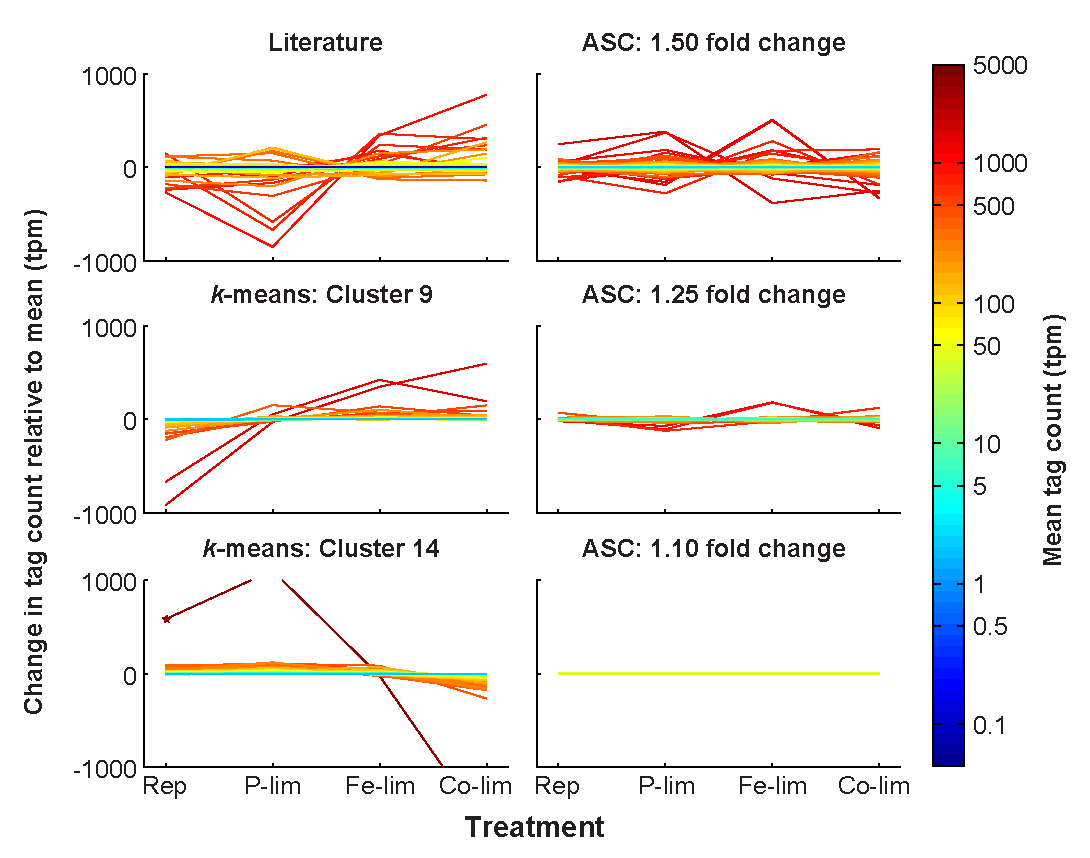
\includegraphics[width=1\textwidth]{Images/C2_Figure1_v6.pdf}
    \caption[Expression patterns of putative reference genes]{Expression patterns of putative reference genes identified through literature-based searches, $k$-means clustering, and ASC analysis. Through literature-based searches, a total of 101 genes homologous to reference genes from previous studies on plants and algae were identified in \textit{T. pseudonana} and plotted to indicate deviation and mean TPM (Literature). $K$-means clustering was applied to the 7380 genes and Cluster 9 (243 genes) and Cluster 14 (466 genes) possessed the genes with the most stable expression pattern across the four treatments. Genes from these clusters are plotted to indicate deviation and mean TPM ($k$-means: Cluster 9; $k-$means: Cluster 14). ASC was used to assess statistical significance (post-$p < 0.1$) of fold changes of 1.10, 1.25, and 1.50 for each treatment relative to the replete control. Genes from these fold change bins are plotted to indicate deviation and mean TPM (ASC: 1.50 fold change; ASC: 1.25 fold change; ASC 1.10 fold change). For a fold change of 1.10, two genes, both hypothetical proteins, (NCBI: 7446346 and 7452192) passed the post-$p < 0.1$ cutoff, and represent the most stable genes based on the ASC analysis (\ref{DS23}). For each of the six classes of putative reference genes, tag counts were normalized to total library size (in TPM) and are plotted relative to the mean for each of the four treatments: Replete (Rep), P-limited (P-lim), Fe-limited (Fe-lim), and co-limited (Co-lim). The color of the line correlates to the mean normalized tag count. A star marks a gene (NCBI: 7451632) in Cluster 14 that is not on the scale of expression for P-limited (1104.7 TPM) and co-limited (-1664.9 TPM) treatments. }
  \label{fig:c2f1}
\end{figure}

The high-throughput transcript dataset was analyzed with $k$-means clustering. Prior to performing $k$-means cluster analysis, FOM optimization was run and found to be minimized at $k=1$5. Thus, $k$-means analysis was run under the Pearson correlation coefficient for $k=15$, yielding 15 clusters, for which the intra-cluster variation was minimized (Figure \ref{fig:a1f2}). Of the 15 clusters produced (ranging in size from 162 to 954 genes), Cluster 4 (433 genes), Cluster 9 (243 genes), and Cluster 14 (466 genes) had candidate reference genes based on a low magnitude of change associated with the expression patterns in those clusters (Figure \ref{fig:a1f2}). However, Cluster 4 showed a clear pattern of differential regulation (downregulated in the replete and upregulated in the co-limited), and as such it was not considered to be an optimal candidate cluster and was excluded from additional analyses. Both Cluster 9 and Cluster 14 consisted of genes with a wide range in mean TPM values (1.74 to 4191.91 TPM), with relatively small deviations from the mean value (Figure \ref{fig:c2f1}; \ref{DS22}), which stands in contrast to other clusters that had definite treatment driven expression patterns (Figure  \ref{fig:a1f2}). Despite the relatively small deviations from the mean value, genes in Clusters 9 and 14 displayed both clear patterns of regulation, as demonstrated by the average change in tag count relative to the mean (Figure \ref{fig:c2f2}) and the presence of ``outlier'' genes with differential expression such as NCBI: 7451632, which was downregulated in the co-limited treatment for Cluster 14 (Figure \ref{fig:c2f1}; \ref{DS22}). \par

%Figure 2: Deviation from the mean
\begin{figure}[h!]
  \centering
    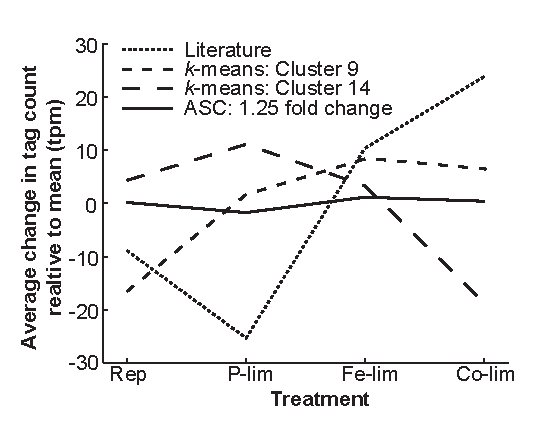
\includegraphics[width=0.65\textwidth]{Images/C2_Figure2_v6.pdf}
    \caption[Average deviation from the mean level of expression for putative reference genes]{Average deviation from the mean level of expression for all genes found with literature-based searches, $k$-means clustering, and ASC analysis of 1.25 fold change. The average change in tag count from the mean expression (TPM) for all the genes identified through literature-based searches for genes homologous to known reference genes from the literature $(n = 101)$, $k$-means clustering from Cluster 9 $(n = 243)$ and Cluster 14 (n = 466), and ASC analysis identifying genes demonstrating a 1.25 fold change with a post-$p < 0.1$ $(n = 179)$. The mean standard deviations for the four cases are as follows: Literature (92.62 TPM), Cluster 9 (41.66 TPM), Cluster 14 (43.12 TPM), and ASC (14.24 TPM). The mean TPM is plotted for the four treatments: Replete (Rep), P-limited (P-lim), Fe-limited (Fe-lim), and co-limited (Co-lim).}
  \label{fig:c2f2}
\end{figure}

Adapting ASC to examine stable expression patterns, genes for which the post-$p$ was less than 0.1 (e.g. had less than a 10\% chance of equaling or exceeding the fold change cutoff) were plotted in three low fold change bins: 1.10, 1.25, and 1.50. A post-$p$ of 0.1 was selected as it optimized the dataset for a wide range of mean gene expression values and provided coverage for each of the fold change bins examined (Table \ref{tab:c2t1}). The number of genes in each of the fold change bins increased with increasing value of fold change. For example, two genes passed the 1.10 cutoff, 179 genes passed the 1.25 cutoff, and 1375 genes passed the 1.50 cutoff. With the increase in the number of genes came an increase in the variation from the mean of the normalized tag counts (Figure \ref{fig:c2f1}; \ref{DS23}). \par
The bin with the 1.10 cutoff had two genes (NCBI: 7446346 and 7452192), which are both hypothetical proteins (Figure \ref{fig:c2f1}). A BLASTn search of 7446346 against the nr NCBI database yielded 69\% identity over 251 base pairs (e-value, 1e-13) to a hypothetical protein (NCBI: CP000544.1) from \textit{Halorhodospira halophila}, a salt-tolerant purple bacterium, and 69\% identity over 232 base pairs (e-value, 1e-12) to a hypothetical protein (NCBI: CP001905.1) from \textit{Thioalkalivibrio} sp. K90mix, also a salt-tolerant chemolithoautotrophic bacteria. BLASTp searches of 7452192 showed the highest identity hits to hypothetical proteins from \textit{Aureococcus anophagefferens} (NCBI: EGB11506.1; 31\% identity; e-value, 2e-21) and from \textit{Chlorella variablis} (NCBI: EFN56803.1; 24\% identity; e-value, 7e-11).\par




The 1.25 fold change bin was used for the identification of candidate reference genes as it offered a larger selection than the 1.10 fold change bin without including genes with increased deviations from the mean, as was the case with the 1.50 fold change bin. Thus, the 1.25 fold change category was the focus of the rest of the analyses (\ref{DS23}). Genes in the 1.25 fold change bin showed a broad range of mean normalized tag counts ranging from 7 to over 1200 TPM with a median of 41.94 TPM, providing for the selection of genes with different levels of constitutive expression in the cell (Figure \ref{fig:c2f1}). Notably, the median of the average tag counts of the genes in the ASC 1.25 fold change bin was 41.94 TPM, which is much higher than that of both Cluster 9 and Cluster 14 with median values of 14.18 TPM and 21.93 TPM, respectively. \par

\begin{landscape}
\begin{table}[h!]
\centering
\caption{Gene counts for the fold change bins of 1.50, 1.25, and 1.10 across posterior probability cutoffs ranging from 0.01 to 0.20.}
\label{tab:c2t1}
\small
\begin{tabular}{|p{2.2cm}|p{1.25cm}|p{1.25cm}|p{1.25cm}|p{1.25cm}|p{1.25cm}|p{1.25cm}|p{1.25cm}|p{1.25cm}|p{1.25cm}|}
\hline
Fold change & \multicolumn{3}{c|}{1.50}                   & \multicolumn{3}{c|}{1.25}                   & \multicolumn{3}{c|}{1.10}                   \\ \cline{1-10} 
Posterior probability                             & Number of genes & Min. TPM & Max. TPM & Number of genes & Min. TPM & Max. TPM & Number of genes & Min. TPM & Max. TPM \\ \hline
post-$p < 0.2$        & 1649            & 2.11        & 1802.38     & 312             & 2.83        & 1281.15     & 8               & 20          & 176.63      \\ \hline
post-$p < 0.1$         & 1375            & 2.22        & 1802.38     & 179             & 7.06        & 1281.15     & 2               & 51.81       & 105.73      \\ \hline
post-$p < 0.05$       & 1127            & 2.83        & 1802.38     & 122             & 20          & 1281.15     & 1               & 105.73      & 105.73      \\ \hline
post-$p < 0.01$        & 801             & 5.69        & 1802.38     & 62              & 20          & 1281.15     & 0               & NA          & NA          \\ \hline
\end{tabular}
\end{table}
\end{landscape}



	Underlying differences in the magnitude and pattern of expression variation across treatments were identified by examining the average tag count change for each reference gene detection method (Figure \ref{fig:c2f2}). If all genes in a group were perfectly constitutively expressed, the average change in tag count relative to the mean observed would be 0 TPM (e.g. the TPM values across all treatments for each of the genes within a group were the same). The average variation from the mean observed in the literature (ranging from -25.34 to 23.84 TPM) highlighted the differential expression across treatments. The average change in tag count relative to the mean in both Cluster 9 (ranging from -16.56 to 8.47) and Cluster 14 (ranging from -18.72 to 11.11 TPM) clearly demonstrated patterns of regulation across treatments (e.g. the upregulation under P-limitation and downregulation under co-limited observed in Cluster 14). In contrast, the average change in tag count relative to the mean observed in the genes identified through ASC (1.25 fold change with post-$p$ < 0.1), which showed a low magnitude of variation (ranging from -1.732 to 1.613 TPM) and a small mean standard deviation across the four treatments (14.24 TPM). Ultimately, the expression patterns of the majority of the genes identified through literature-based searches and $k$-means clustering were more variable across the \textit{T. pseudonana} test treatments, than those genes identified with ASC.\par	
\begin{figure}[h!]
  \centering
    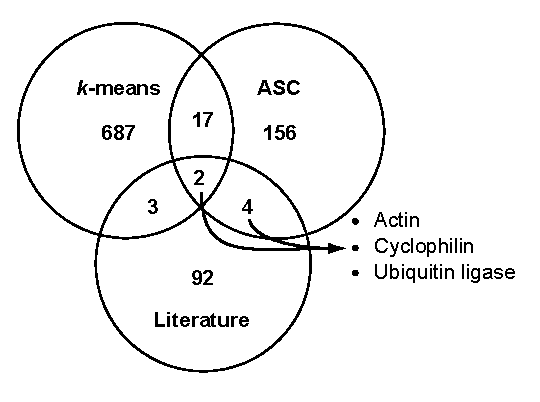
\includegraphics[width=0.75\textwidth]{Images/C2_Figure3_v6_bw.pdf}
    \caption[Comparison of putative reference genes identified through literature, $k$-means clustering, and ASC analysis]{Comparison of possible reference genes found with literature-based searches, $k$-means clustering, and ASC analysis of 1.25 fold change. Venn diagram analysis was used to compare genes identified as candidate reference genes through literature-based homolog searches (totaling 101 genes), with the $k$-means clustering method (genes in Cluster 9 and 14, totaling 709 genes), and with quantitative exclusion by ASC (based on genes demonstrating a 1.25 fold change with a post-$p < 0.1$, totaling 179 genes). The number of genes in each region is reported. The intersection of all ASC and literature-based searches yielded six total genes representing three different gene families: actin (NCBI: 7449411), cyclophilin (NCBI: 7445376), and ubiquitin ligase (NCBI: 7448637, 7450639, 7446724, and 7451971). }
  \label{fig:c2f3}
\end{figure} 
A comparison of the three techniques: literature-based searches, $k$-means cluster selection, and ASC cutoff at 1.25 fold change revealed comparatively few genes in common between the techniques (Figure \ref{fig:c2f3}). Of the 709 genes identified through $k$-means clustering and the 179 genes found through ASC analysis (genes which pass the 1.25 fold change cutoff for post-$p$ < 0.1), 21 genes are shared (Figure \ref{fig:c2f3}), of which six lacked GO annotations or KOG definitions (\ref{DS22}). Between the genes identified through literature and ASC analysis, six genes were held in common; these genes were representative of the general gene classifications: actin (NCBI: 7449411), cyclophilin (NCBI: 7445376), and ubiquitin ligases (NCBI: 7448637, 7450639, 7446724, and 7451971). Only two genes (NCBI: 7448637 and 7446724) were found in common amongst all three methods of reference gene selection, both of which were annotated as putative ubiquitin ligases (\ref{DS21}). \par



\section{Discussion}
	Prior to the availability of high-throughput molecular datasets, reference genes for non-model organisms were selected based on literature reports of stably expressed genes in model organisms. With non-model organisms such as eukaryotic phytoplankton this task is particularly difficult, as stably expressed genes are not readily apparent in the relatively limited molecular literature specific to these organisms. Often the selection of a reference gene relies on information from distantly related organisms under dissimilar conditions, leading to extensive validation work \citep{McDonald2010, Whitney2011a}. Herein, we compared the efficacy of reference gene selection based on the literature as compared to verifiable selection through $k$-means clustering and ASC analysis of high-throughput transcriptome data in \textit{T. pseudonana} across four nutrient treatments (replete, P-limited, Fe-limited, and co-limited). These treatments are of environmental relevance as both P and Fe are major drivers of diatom physiological ecology and consequently carbon fixation \citep{Moore2004}. Additionally, P and Fe often occur concurrently at very low concentrations in marine systems and have been found to be independently co-limited, or mutually exclusive biochemically \citep{Saito2008}.\par
    Our literature-based search of relative gene expression studies from 12 algae and plants yielded 18 general reference gene categories, for which 101 homologs in the \textit{T. pseudonana} genome were identified (\ref{DS21}). While some of these genes demonstrated stable expression (e.g. actin, cyclophilin, and ubiquitin conjugating enzymes), the vast majority displayed some form of differential expression in the treatments examined herein. Furthermore, there was considerable heterogeneity of expression among the different gene copies of actin, cyclophilin, and ubiquitin conjugating enzymes, demonstrating that not all genes within a gene family are stably expressed. These data underscore that a literature-based selection of reference genes necessitates validation across all treatments of interest \citep{Vandesompele2002, Pfaffl2004}. \par
	Differential expression patterns in high-throughput datasets are often analyzed with clustering methods, such as hierarchical or $k$-means clustering \citep{Dhaeseleer2005}. Rather than using a clustering method for the identification of differential expression patterns, here it is applied to identify constitutively expressed genes. The $k$-means clustering algorithm was chosen as it is a top-down or partition-based approach to gene clustering that is not hierarchical and requires few assumptions about the data \citep{Hartigan1979}. Several of the 709 putative reference genes identified by $k$-means analysis (from Clusters 9 and 14) were clearly differentially regulated, with large deviations from the mean expression level. The presence of outliers is to be expected using the $k$-means method, for it is a pattern-based method and all genes must be placed into one of the partitioned $k = 15$ clusters. Thus, optimal placement of a gene is not always guaranteed. As with a finite number of clusters, the assignment of a gene is often forced. For example, even genes in Cluster 9 and 14 were subject to strong patterns of regulation, with both clusters demonstrating large average changes in tag count relative to the mean tag count. Arguably, it is better to select a reference gene from a pool of genes that do not share the same pattern of regulation. Therefore, genes uncovered via $k$-means clustering must be manually surveyed to exclude genes with large deviation prior to the selection of a candidate reference gene.\par
	In lieu of clustering approaches, other studies have used statistical parsing of ESTs in tomato plants \citep{Coker2003} and Affymetrix whole-genome GeneChip data from \textit{A. thaliana} \citep{Czechowski2005} and humans \citep{DeJonge2007a} to identify reference genes that have small deviations from the mean of replicated treatments. In contrast to these and other statistical methodologies typically applied to high-throughput sequence data with replication, the Bayesian approach to gene expression analysis, ASC, allowed for selection of candidate genes based on a statistical cutoff rather than cardinality. Though typically used for the identification of differentially expressed genes, the function of ASC was reversed in this study by lowering the post-$p$ cutoff. Genes for which post-$p < 0.1$ for a specified fold change were targeted, meaning that genes that were unlikely to have made that fold change were selected. The 1.25 fold change bin yielded the most options for candidate reference genes without sacrificing stability of expression (as was seen in the 1.50 fold change bin). \par
	ASC provides a method of identifying reference genes with expression levels similar to those of target genes. For example, the mean normalized tag counts of genes identified using ASC were broad (from 7 to over 1200 TPM), providing the opportunity for reference gene expression to be generally matched with target gene expression. Current studies frequently employ reference genes for endogenous control that have very high levels of expression across all treatments, such as ACT1 (NCBI: 7449411) in \textit{T. pseudonana} (which has a mean expression value of 1024.1 TPM in this data set), yet these highly expressed genes might not be optimal for studies of genes with low levels of expression or when multiplexing targets in probe-based RT-qPCR analysis. \par
	High-throughput transcript datasets also allow the selection of reference genes to move beyond the confines of gene annotation and previously identified reference genes. In fact, the two genes with the most stable expression in the 1.10 fold change bin are hypothetical, with no clear annotation. Of the 179 genes that passed the 1.25 fold change cutoff with ASC, 44 lacked both GO and KOG annotations. A large percentage of the 11,390 genes in the \textit{T. pseudonana} genome are annotated as hypothetical proteins \citep{Armbrust2004, Mock2008}, and here we show a number of them are stably expressed across the target conditions. This has been seen with model organisms, where a good majority of constitutively expressed genes fall outside the bounds of preconceived ``housekeeping'' genes \citep{Czechowski2005, DeJonge2007a}. By using a Bayesian approach such as ASC, hypothetical proteins can be chosen as reference genes. \par
    Comparison of the putative reference genes recovered using ASC to previous studies served to cross-validate the ASC approach. Actin (ACT1, NCBI: 7449411) has been validated in the literature as a suitable reference gene for relative expression studies of \textit{T. pseudonana} under Fe-limitation \citep{Whitney2011a}, a treatment considered in this study, and was one of the 179 genes passing the ASC 1.25 fold change cutoff. Additionally, only five of the 179 genes with stable expression found with ASC were identified as differentially expressed in a study of \textit{T. pseudonana} under additional treatments to those described here (e.g. nitrogen limitation, silica limitation, etc.) \citep{Mock2008} (\ref{DS24}). Of the five, only one gene (NCBI: 7451974) was identified as differentially expressed under Fe-limitation, a condition examined in this study. Taken together, this validates the genes identified with ASC using alternative data and methods, and suggests that the ASC-detected genes are globally stable across many different conditions for \textit{T. pseudonana}. However, one of the two genes identified in the 1.10 fold change bin (NCBI: 7446346) was identified as significantly down-regulated under nitrogen limitation by \citet{Mock2008}. This highlights the importance of validating genes across all treatments of interest prior to their use as reference genes. \par
	Notably, the $k$-means and ASC dataset revealed only 21 genes in common. The 179 genes found through ASC were, in fact, distributed fairly evenly across all of the 15 clusters. The lack of intersection observed between the two datasets is likely related to the parsing ability inherent in $k$-means clustering. The $k$-means approach is highly driven by patterns of differential regulation, but does not consider the significance of that regulation (e.g. genes that are not significantly upregulated are placed in a cluster with genes that are significantly upregulated). Thus, the stably expressed genes that were identified by ASC, though not displaying major patterns of regulation, were clustered based on minor patterns in variation of gene expression. Therefore, while $k$-means clustering provides a global view of commonalities in gene expression patterns, ASC is more robust at identifying reference genes.\par
	Eight genes were common between the ASC and literature-based searches, which were distributed across three general gene classes: actin (NCBI: 7449411), cyclophilin (NCBI: 7445376), and ubiquitin ligases (NCBI: 7448637, 7450639, 7446724, and 7451971). For those interested in identifying suitable reference genes for studies in \textit{T. pseudonana} but lack transcriptome datasets across the treatments of interest, these eight genes may serve as good tentative reference genes as they are verified in this study and have been identified as stable in many other organisms under many conditions. In particular, ubiquitin ligases/conjugating enzymes have been used as reference genes in several studies involving other algae, namely, \textit{Aureococcus anophagefferens}, \textit{Phaeodactylum tricornutum}, and \textit{Prorocentrum minimum} \citep{Siaut2007, McGinn2008, Guo2012, Wurch2011, Berg2008}, and with further analysis may represent particularly good reference genes in the phytoplankton. \par
	Sequence-based transcriptome profiling has become an increasingly useful method for gene discovery and differential expression analysis. Yet, RT-qPCR is still valuable for the examination of detailed trends in expression in both culture and field studies. Here we show that the application of ASC and, to a lesser extent, $k$-means clustering can be used to successfully screen transcriptome data for potential reference genes. The isolation of candidate reference genes using ASC with the 1.25 fold change cutoff for post-$p < 0.1$ was more robust and stringent at excluding differentially expressed genes than both the literature-based searches and $k$-means clustering. Based on these data for \textit{T. pseudonana}, it was shown that ACT 1 and ubiquitin ligase may be useful reference genes. Yet, in addition to these common reference genes, the data demonstrate that there are many more stably expressed genes (both annotated and hypothetical) to choose from for expression studies in this and potentially other diatoms. Notably, this survey focused only on variation in P and Fe supply, so these genes may not transfer to studies of other nutritional drivers or other physical forces, such as light intensity or temperature. As more transcriptome data are generated for phytoplankton, ASC can be employed without sequence replicates, to identify reference genes for other phytoplankton under various conditions. Additionally, the suite of genes identified through these analyses might allow for better multi-gene normalization analysis that would provide for the detection of smaller fold changes with certainty \citep{Vandesompele2002, Czechowski2005}.\par




%% This is an example first chapter.  You should put chapter/appendix that you
%% write into a separate file, and add a line \include{yourfilename} to
%% main.tex, where `yourfilename.tex' is the name of the chapter/appendix file.
%% You can process specific files by typing their names in at the 
%% \files=
%% prompt when you run the file main.tex through LaTeX.
\chapter{Metatranscriptome analyses indicate resource partitioning between diatoms in the field}
\label{chap:3}

\raggedbottom
%\begin{singlespace}
%Harriet Alexander$^{1,2}$, Bethany D. Jenkins$^{3,4}$, Tatiana A. Rynearon$^{3}$, Sonya T. Dyhrman$^{5}$\\
%\\
%$^{1}$ MIT-WHOI Joint Program in Oceanography/Applied Ocean Science and Engineering, Cambridge, MA 02139, USA\\
%$^2$ Biology Department, Woods Hole Oceanographic Institution, Woods Hole, MA 02543, USA\\
%$^3$ Graduate School of Oceanography, University of Rhode Island, Narragansett, RI 02882, USA\\
%$^4$ Department of Cell and Molecular Biology, University of Rhode Island, Kingston, RI 02881, USA\\
%$^5$ Department of Earth and Environmental Sciences Lamont-Doherty Earth Observatory, Columbia University, Palisades, NY 10964\\
%\\
{\let\thefootnote\relax\footnotetext{This chapter was originally published as Alexander, H., Jenkins, B.D., Rynearson, T.A., and Dyhrman, S.T. (2015). \href{http://www.pnas.org/content/112/17/E2182.long}{Metatranscriptome analyses indicate resource partitioning between diatoms in the field}. \emph{Proc. Natl. Acad. Sci. U. S. A.} 112:17, E2182-E2190.}}
{\let\thefootnote\relax\footnotetext{H.A., B.D.J., T.A.R., and S.T.D. designed research; H.A., B.D.J., T.A.R., and S.T.D. performed research; H.A. contributed new reagents/analytic tools; H.A. analyzed data; and H.A., B.D.J., T.A.R., and S.T.D. wrote the paper.}}
{\let\thefootnote\relax\footnotetext{The supplemental figures, tables, and data sheets for this chapter can be found in \cref{sec:app3}.}}

%\end{singlespace}
\clearpage
\section{Abstract}
Diverse communities of marine phytoplankton carry out half of global primary production. The vast diversity of the phytoplankton has long perplexed ecologists, as these organisms coexist in an isotropic environment while competing for the same basic resources (e.g. inorganic nutrients). Differential niche partitioning of resources is one hypothesis to explain this ``paradox of the plankton,'' but it is difficult to quantify and track variation in phytoplankton metabolism \textit{in situ}. Here we use quantitative metatranscriptome analyses to examine pathways of nitrogen (N) and phosphorus (P) metabolism in diatoms that co-occur regularly in an estuary on the east coast of the US (Narragansett Bay). Expression of known N and P metabolic pathways varied between the two diatom species, indicating apparent differences in resource utilization capacity that may prevent direct competition.  Nutrient amendment incubations skewed N:P ratios, elucidating nutrient responsive patterns of expression, and facilitating a quantitative comparison between diatoms. The resource-responsive (RR) gene sets deviated in composition from the metabolic profile of the organism, being enriched in genes associated with N andeP metabolism. Expression of the RR gene set varied over time and differed significantly between diatoms, resulting in opposite transcriptional responses to the same environment. Apparent differences in metabolic capacity and the expression of that capacity in the environment suggest that diatom-specific resource partitioning was occurring in Narragansett Bay. This high-resolution approach highlights the molecular underpinnings of diatom resource utilization and how co-occurring diatoms adjust their cellular physiology to partition their niche space. 
 
\section{Introduction}
The stability and primary productivity of ecosystems has long been linked to the diversity of primary producers \citep{Elton1958, Cardinale2012}. This is well documented in terrestrial systems \citep{Naeem1994, Tilman2001, Cadotte2013, Balvanera2006, Tilman1996} and is increasingly being established for marine systems \citep{Behl2011, Striebel2009, Steiner2005, Ptacnik2008}. Marine phytoplankton generate roughly half of global primary production \citep{Nielsen1960, Strickland1965, Field1998} and play a critical role in oceanic ecosystem structure and function. Within the phytoplankton, the diatoms generate an estimated 40\% of marine primary production \citep{Nelson1995}. Thus diatoms alone exert profound influence over marine primary production and global carbon (C) cycling, particularly in coastal margins and estuaries. \par
Phytoplankton are extremely diverse, with over 5,000 described species \citep{Sournia1991, Tett1995, Mann1996}. This dramatic level of taxonomic diversity in the plankton is difficult to resolve with the apparently limited number of niches in the pelagic habitat, as these organisms compete for the same two basic resources: light and nutrients. As was highlighted by \citet{Hutchinson1961}, the phytoplankton violate Gause's law of competitive exclusion, which posits that two organisms competing for the same resources cannot coexist. Much thought has gone towards identifying the cause of the ``paradox of the plankton'' and include explanations such as ``contemporaneous disequilibrium'' of patchy phytoplankton distributions \citep{Richerson1970}, life history differences \citep{Huisman2001}, species oscillations \citep{Huisman1999}, environmental fluctuation \citep{Roy2007}, intra-specific variation \citep{Menden-deuer2014}, and differential niche partitioning \citep{Connel1980}. Of these potential factors, one of the most difficult to directly observe in the plankton is niche partitioning. Different species may have unique strategies that allow them to specialize on certain resources or nutrient forms, and species may have different responses to resource shifts that allow them to avoid competition. Such specialization in eco-evolutionary strategy may underlie the ``winner-loser'' dynamics observed in productive estuaries and coastal systems, yet resolving patterns of species-specific resource metabolism in the field remains a central challenge.\par
It is accepted that the macronutrients N and P are central to the structuring of phytoplankton communities across large spatial and temporal scales \citep{Margalef1963, Follows2007, Johnson2006b}, and that phytoplankton compete for nutrients in the natural environment \citep{Sommer1983, Sommer1985}. Studies focused on nutrient geochemistry, and phytoplankton quotas or uptake have emphasized the importance of nutrients to community dynamics, but these do not generally examine resource partitioning between individual species \citep{Hutchins1999, Zubkov2003}. Transcriptional studies provide species-specific resolution, but few studies have examined the global expression of nutrient metabolism pathways in the field \citep{Marchetti2012a} or in organisms lacking a fully sequenced genome \citep{Frischkorn2014, Moustafa2010}, and as a result, the mechanistic underpinnings of phytoplankton resource metabolism \textit{in situ} are not well understood. \textit{In situ} global gene expression analyses (metatranscriptome profiling) are a means for elucidating a species' metabolic capacity and examining patterns in resource utilization potential through time by tracking the expression of species' resource-responsive genes. When simultaneously applied to multiple species in a sample, this can resolve differences in the expressed gene compliment and how it is modulated, which may reflect resource partitioning of phytoplankton niche space \citep{Gifford2013}. For example, this approach has uncovered species-specific expression of genes for the transport of organic compounds \citep{Poretsky2010, Rinta-Kanto2012a, Gifford2011}, highlighting potential differences in resource partitioning. Although increasingly critical for identifying resource utilization in the bacterioplankton, metatranscriptome profiling has only recently been used to examine resource utilization in coastal eukaryotic phytoplankton populations \citep{Dupont2015}, largely due to challenges in quantifying a transcriptional response in a mixed population and until recently, the lack of reference genomes and transcriptomes for determining the origin of the transcriptional response. Co-occurring phytoplankton may possess different metabolic capabilities and responses to resource availability, which may then enable resource partitioning and the segregation of the fundamental niche or the realized niche. Knowledge of if and how these organisms modulate their niche space would allow predictive models to better resolve species distribution and ecosystem structure and function in the future ocean \citep{Follows2007}.\par
Herein we examined pathways of resource metabolism between two co-occurring diatoms from the genera \textit{Thalassiosira} and \textit{Skeletonema}, sampled from a time-series site in Narragansett Bay. Narragansett Bay is a highly productive and dynamic estuarine environment on the east coast of the United States with an estimated bay-wide average net production of $269\ gC\ m^{-2}\ yr^{-1}$ \citep{Oviatt1981}. Quantitative metatranscriptomic techniques were developed and used to: 1) assign taxonomic designation, 2) assess and track changes in known metabolic capacity through quantitative molecular fingerprinting (QMF), 3) statistically identify the resource responsive gene set, and 4) proportionalize the expression of resource-responsive genes to track species-specific responses through time, using standardized transcriptional differentiation scores ($STD$). This multifaceted computational approach enabled the unprecedented resolution of the unique strategies these two diatoms use for resource acquisition. \par
\section{Materials and Methods}
\subsection{Experimental set up and sample collection}
Surface seawater was collected and sampled for total community RNA at the long-term sampling site in Narragansett Bay, RI (Station II, $41^\circ 34^\prime 07^{\prime \prime}$ N, $71^\circ 23^\prime 31^{\prime \prime}$ W) during 2012 (16 May, 21 May, 30 May, 4 June, and 8 June, here called S1 through S5) in conjunction with the weekly time-series sampling effort. To diminish the influence of diel signals, samples were collected and processed between 0830 and 0900 local time. Near surface water was collected in an acid-washed carboy and then filtered onto polycarbonate filters (5.0 $\mu$m pore size, $47mm$) using a peristaltic pump. Filters were then placed in cryovials and stored in liquid nitrogen until RNA extraction. In this manner all samples were preserved within 15 minutes of collection. In addition to sampling for total community RNA, phytoplankton abundance was measured as part of the long-term weekly survey \citep{Furnas1983, Furnas1982}.\par
A nutrient amendment incubation experiment was performed on 30 May 2012, with S3 representing the t = 0 of the experiment. Water collected in conjunction with S3 was pre-filtered through $200 \mu m$ mesh to remove large zooplankton grazers and placed into acid washed 2.5-L bottles. Triplicate bottles were then amended with nutrients to create five treatments: +N, +P, -N, -P, and ambient control. The +N and +P treatments were designed to eliminate the N and P stress signals, respectively, while the -N and -P treatments were supplemented with everything except the nutrient in question (e.g. the -N treatment was amended with P, Si, Fe, and vitamins), to force the draw down of N and P, respectively (\cref{tab:a3t2}). N and P amendment concentrations were selected to be approximately 10x the seasonal average ambient N and P concentrations in the surface waters of Narragansett Bay measured at Station II. Silica, Fe, and f/5 vitamin amendments were made in proportion to the f/5 media ratios \citep{Guillard1975}. Bottles were placed in a flow-through incubator at ambient temperatures and PAR to mimic the collection depth. The incubation was run for 48 hours, at which point all treatments were sampled for total community RNA as described above by filtering and snap- freezing $2L$ of biomass from each replicate bottle. \par
\subsection{RNA extraction and sequencing}
Filters from triplicate bottles, representing approximately $6L$ of water, were pooled by treatment and extracted for each of the \textit{in situ} and incubation experiment samples. RNA was extracted from individual filters with the RNAeasy Mini Kit (Qiagen), following a modified version of the yeast protocol. Briefly, lysis buffer and RNA-clean zircon beads were added to the filter and samples were vortexed for 1 minute, placed on ice for 30 seconds, and then vortexed again for 1 minute. Samples were then processed following the yeast protocol. The resulting RNA was eluted in water and then treated for possible DNA contamination using TURBO DNA-free Kit (Ambion) following the Rigorous Dnase protocol. RNA from each triplicate was then pooled by sample or treatment, using the RNA Cleanup Protocol from the RNAeasy Mini Kit (Qiagen). The total RNA ( $>1000$ ng for each sample) was then enriched for eukaryotic mRNA through a poly-A pull down onto oligo-dT beads. The resulting enriched RNA sample then went through library preparation with the Illumina TruSeq RNA Prep Kit (Illumina). Libraries were sequenced at the Columbia University Genome Center (New York, New York) with an Illumina HiSeq2000. Each sample was sequenced to produce $\sim 60$ million, 100 base pair, paired end reads (\cref{tab:a3t1}). Raw sequence data quality was visualized using FastQC \citep{Andrewsa} and then cleaned and trimmed using Trimmomatic v 0.27 (paired end mode; 6-base pair wide sliding window for quality below 20; minimum length 25 base pair) \citep{Lohse2012}. Environmental sequence reads are available at the NCBI under accession number \href{http://www.ncbi.nlm.nih.gov/sra/?term=SRP055134}{SRP055134}. 
\subsection{Transcriptome and genome mapping}
To assign taxonomic identification to the reads a database was created from transcriptomes made publicly available as of 17 March 2014 through the Marine Microbial Eukaryote Transcriptome Sequencing Project (MMETSP). In total, 401 transcriptomes from 209 species or cultured isolates were collected. Like-species transcriptomes were combined (regardless of strain or condition) using CD-HIT-EST (98\% identity; word size of 9). The resulting clustered set of transcripts was considered to be the representative transcriptome for the species or cultured isolate. The 209 transcriptomes created in this manner were concatenated to form a comprehensive species-level transcriptome database from the MMETSP library. Due to the large size of the resulting MMETSP database, trimmed reads were mapped to the MMETSP using the Burrows-Wheeler Aligner (BWA) \citep{Li2010} and then counted using the HTSeq 0.6.1 package \citep{Anders2014}.\par 
Transcriptomes from two ecologically relevant diatom species in Narragansett Bay were selected: \textit{Skeletonema} costatum RCC1716 (MMETSP0013, accessed from the publicly available transcriptome databases, Moore Foundation Marine Microbiology Initiative-supported Marine Microbial Eukaryote Transcriptome Sequencing Project, National Center for Genome Resources) and \textit{Thalassiosira rotula} CCMP3096 (a custom assembly available at EBI, accession number Hx2000045970). These transcriptomes were individually clustered using CD-HIT-EST (parameters: -c 0.98, -n 9) \citep{Li2006}. The resulting clustered set of transcripts was then concatenated to form a reference transcriptome database. Trimmed reads from the field and incubation samples were mapped to this transcriptome database using Bowtie2 v 2.2.1 (parameters: -a -sensitive) \citep{Langmead2012}. As a point of comparison, reads were also mapped using Bowtie2 v2.2.1 under the same parameters to the genome of the model centric diatom species, \textit{Thalassiosira pseudonana} CCMP1335 (v3.0), an organism not known to be abundant in Narragansett Bay. Mapped reads were then counted by transcript using the HTSeq 0.6.1 python package (parameters: -m union -s no) \citep{Anders2014}. Reads aligning to more than one full transcript were not counted. KEGG pathways were assigned to the assembled sequences using the online KEGG Automatic Annotation Server (KAAS), using the bi-directional best-hit (BBH) method to obtain KEGG Orthology annotations. In this study, only genes with a normalized count (NC) (raw count / total number of genes mapped to an organism) of at least 2 tags per million (TPM) in at least one of the field or incubation samples were included, thus limiting the sample set to 4318 genes for \textit{T. rotula} (19.3\% of the transcriptome) and 20921 genes for \textit{Skeletonema} spp. (75.6\% of the transcriptome). This difference in coverage is directly related to their relative abundance in the population.
\subsection{Transcriptome clustering}
To assess relatedness of genes within \textit{Skeletonema} spp. and \textit{T. rotula}, the transcriptomes were translated using \href{http://proteomics.ysu.edu/tools/OrfPredictor.html}{ORF Predictor} using a reference BLASTx alignment against the NCBI database with an 1e-5 cutoff \citep{Min2005}. These translated peptide sequences were then combined with the translated proteins from the diatom genomes \textit{Fragilariopsis cylindrus} CCMP1102 v1.0, \textit{Phaeodactylm tricornutum} CCMP632 v2.0, \textit{Pseudo-nitzschia multiseries} CLN-47 v1.0, and \textit{Thalassiosira pseudonana} CCMP1335 v3.0, which were collected from the Joint Genome Institute \href{http://genome.jgi-psf.org}{JGI} database. A protein similarity network was then created using EGN, a software program that automates the reconstruction of gene networks from protein sequences through reciprocal BLASTp analysis (e-value <1e-5, hit identity threshold: 20\%, best-reciprocal threshold of best e-value: 5\%, minimal match coverage threshold: 90\%) \citep{Halary2013, Halary2010}. Networks were then visualized and manipulated using Cytoscape 3.0, where the layout of the network was produced using an edge-weighted spring-embedded model based on e-value, meaning that genes that are closer together are more similar \citep{Smoot2011, Saito2012}. Known RR genes from previous transcriptome studies of the diatom species, \textit{T. pseudonana}, were selected for analysis: 1) the P-responsive gene, Thaps\_24435, a NPT \citep{Dyhrman2012} and 2) the N-responsive gene, Thaps\_25299, an assimilatory nitrate reductase \citep{Bender2014}. 
\subsection{Identification of stable and nutrient-responsive genes}
Intercomparison of nutrient-incubation experiments enabled the identification of both nutrient-responsive genes and stably expressed reference genes for \textit{T. rotula} and \textit{Skeletonema} spp.. For each organism, RR genes were identified by comparing the counts for that organism in +N to the -N incubation and the +P to the -P incubation, respectively, using Analysis of Sequence Counts (ASC), an empirical Bayes method, which estimates the prior distribution from the data, itself \citep{Wu2010}. ASC analyses were run using raw count data from each species separately. Genes were considered to be differentially regulated between treatments if for a fold change of 2.0 the posterior probability (post-$p$) was greater than 0.95 \citep{Dyhrman2012}. After surveying the output of several different post-$p$ cutoffs (\cref{fig:a3f11}), stable genes were identified using ASC as described by \citet{Alexander2012} through pairwise comparisons of each of the incubation treatments (fold change of 1.25, post-$p < 0.1$). 
\subsection{Normalization of metatranscriptome data}
Counts from the field were first normalized to the sequences belonging to the species in the library (Equation \ref{eq:NC}). For a particular species, $c$, the number of reads mapping to a gene $g$, $c_{i,g}$, was normalized to the sum of all the counts across all genes for that organism yielding the normalized count, $NC_{i,g}$, similar to normalization techniques used for metatranscriptome data \citep{Marchetti2012a, Ottesen2011}. 
%Equation 1. Normalized counts
\begin{equation}
	\label{eq:NC}
	NC_{i,g} = \frac{c_{i,g}}{\sum \limits_{g \epsilon G} c_{i,g}}
\end{equation}

From hence forth, only genes for which $NC > 2$ TPM in at least one sample (incubation or field) were considered. To facilitate interspecies comparisons, the NC was normalized to the geometric mean of the set of stable reference genes, $R$, yielding a stable gene normalized count ($SGNC$). The calculation of $SGNC$ (Equation \ref{eq:SGNC}) for transcriptome data, while a novel application to metatranscriptome analysis, was designed to emulate the normalization used in qRT-PCR studies \citep{Vandesompele2002}. \par
%Equation 2. Stable gene normalized counts
\begin{equation}
	\label{eq:SGNC}
 	SGNC_{i,g}=\frac{NC_{i,g}}{\left ( \prod \limits^{R} NC_{i,g} \right ) ^{1/R}}
\end{equation}

The nutrient responsive genes identified as differentially expressed in the nutrient incubations (\cref{tab:a3t2}) were then selected for investigation in the field metatranscriptomes (S1 through S5). The $SGNC$ from the field for these nutrient-related genes were bounded by the $SGNC$ from like nutrient incubations to calculate the standardized transcriptional differentiation score for N ($STD_N$) (Equation \ref{eq:STDN}) and P ($STD_P$) (Equation \ref{eq:STDP}).\par 

%Equation 3. Standardized transcriptional differentiation score (nitrogen)
\begin{equation}
	\label{eq:STDN}
	STD_N = \frac{SGNC_{field} - SGNC_{+N}}{SGNC_{-N} - SGNC_{+N}} 	
\end{equation}

%Equation 4. Standardized transcriptional differentiation score (phosphorus)
\begin{equation}
	\label{eq:STDP}
	STD_N = \frac{SGNC_{field} - SGNC_{+P}}{SGNC_{-P} - SGNC_{+P}} 	
\end{equation}

For example, in calculating $STD_N$, the $SGNC_{field}$ is put in the range of the $SGNC_{+N}$ and $SGNC_{-N}$. By consequence, if the $STD_N$ for a gene in the field equals zero it is more similar in expression to the +N treatment and if it equals one it is more similar in expression to the -N treatment. As such, a plot $STD_N$ against $STD_P$, can divide the space into two main theoretical quadrants N:P > Redfield ($STD_P > 1$ and $STD_N < 0$) and N:P < Redfield ($STD_N > 1$ and $STD_P < 0$) (\cref{fig:a3f8}). The total number of genes falling into each of the quadrants were counted by varying the bounds considered: the N:P > Redfield ratio quadrant ($STD_P > C$; $STD_N < C$, for $0.25 < C < 0.75$) and the N:P < Redfield ratio quadrant ($STD_P < C$; $STD_N > C$, for $0.25 < C < 0.75$). To conservatively approximate variation, the value of C was varied over 10 different values and the average and standard deviation for the percentages of genes falling into each of the quadrants was quantified. Similarity of data between species by quadrant was assessed using an analysis of variance (ANOVA) with a generalized linear model. The results from a post hoc Tukey test show the divergence of species across time ($p < 0.05$).

\section{Results and Discussion}
\subsection{Samples and sequencing}
Narragansett Bay has seasonal blooms of diatoms which have been monitored through weekly cell counts for over 50 years at a long-term time series station \citep{Borkman2009, Li1998}. Five eukaryotic surface metatranscriptome samples were taken from surface seawater collected during May and June of 2012 at the time-series site yielding over 358 million 100 base pair, paired end cDNA reads from the field (S1-5) (\cref{tab:a3t1}). In conjunction with these field-based surveys, a nutrient amendment incubation experiment was performed with natural communities on 30 May 2012 (S3) to drive the community towards opposite extremes in the nitrogen (N): phosphorus (P) ratio (Redfield ratio) (\cref{tab:a3t2}). Eukaryotic metatranscriptomes from the five incubation treatments produced over 264 million 100 base pair, paired end cDNA reads (\cref{tab:a3t1}).\par

To assign taxonomic designation, sequences from the time series were conservatively mapped (such that if a read mapped to more than one gene it was discarded) to a sequence library containing all assembled sequences and annotations generated through the Marine Microbial Eukaryotic Transcriptome Sequencing Project (MMETSP) \citep{Keeling2014} which were public as of 17 March 2014. The custom sequence library contained 401 transcriptomes across 209 species or cultured isolates. Between 62 to 71\% of reads from the \textit{in situ} samples mapped to the MMETSP database with diatoms dominating the libraries, representing 30 to 46\% of the total mapped reads (\cref{fig:c3f1}). The peak in diatom representation coincided with a bloom of \textit{Skeletonema} spp. detected in time-series cell counts (\cref{fig:a3f1}), and a period of historical overlap between the \textit{Skeletonema} and \textit{Thalassiosira} genera. \textit{Skeletonema} and \textit{Thalassiosira} were well represented during the time period studied in both mapped RNA (\cref{fig:c3f1}) and cell counts (\cref{fig:a3f1}). \textit{T. rotula} was present but at low abundance during the time-series, while \textit{Skeletonema} spp. was abundant, with sampling spanning a bloom of \textit{Skeletonema} (>10,000,000 cells L$^{-1}$), with peak cell densities in S2 (21 May 2012) (\cref{fig:a3f1}). As such, subsequent analyses were focused on these two groups by remapping the data to representative transcriptomes: \textit{T. rotula} and \textit{S. costatum} (\cref{tab:a3t1}). \textit{S. costatum} was chosen as it was the transcriptome from the genus \textit{Skeletonema} that recruited the most hits in the MMETSP database. Because \textit{Skeletonema} is known to include morphologically cryptic species that can only be identified by scanning electron microscopy \citep{Sarno2005, Zingone2005, Smayda2011}, it is referred to here as \textit{Skeletonema} spp. for clarity. Up to 17.5 and 54.9\% of reads from a single sample mapped to \textit{T. rotula} and \textit{S. costatum}, respectively. As a point of comparison, reads were also mapped to the genome of a second Thalassiosirid, \textit{T. pseudonana}, a diatom that is not known to be abundant in Narragansett Bay (\cref{tab:a3t1}). Though displaying high identity with the 18S rDNA to \textit{T. rotula} and \textit{S. costatum} (96\% and 93\% identity, respectively), less than 1\% of the metatranscriptome reads mapped \textit{T. pseudonana} (\cref{tab:a3t1}), highlighting the specificity of the approach. 

% Figure 1
\begin{figure}[h!]
  \centering
    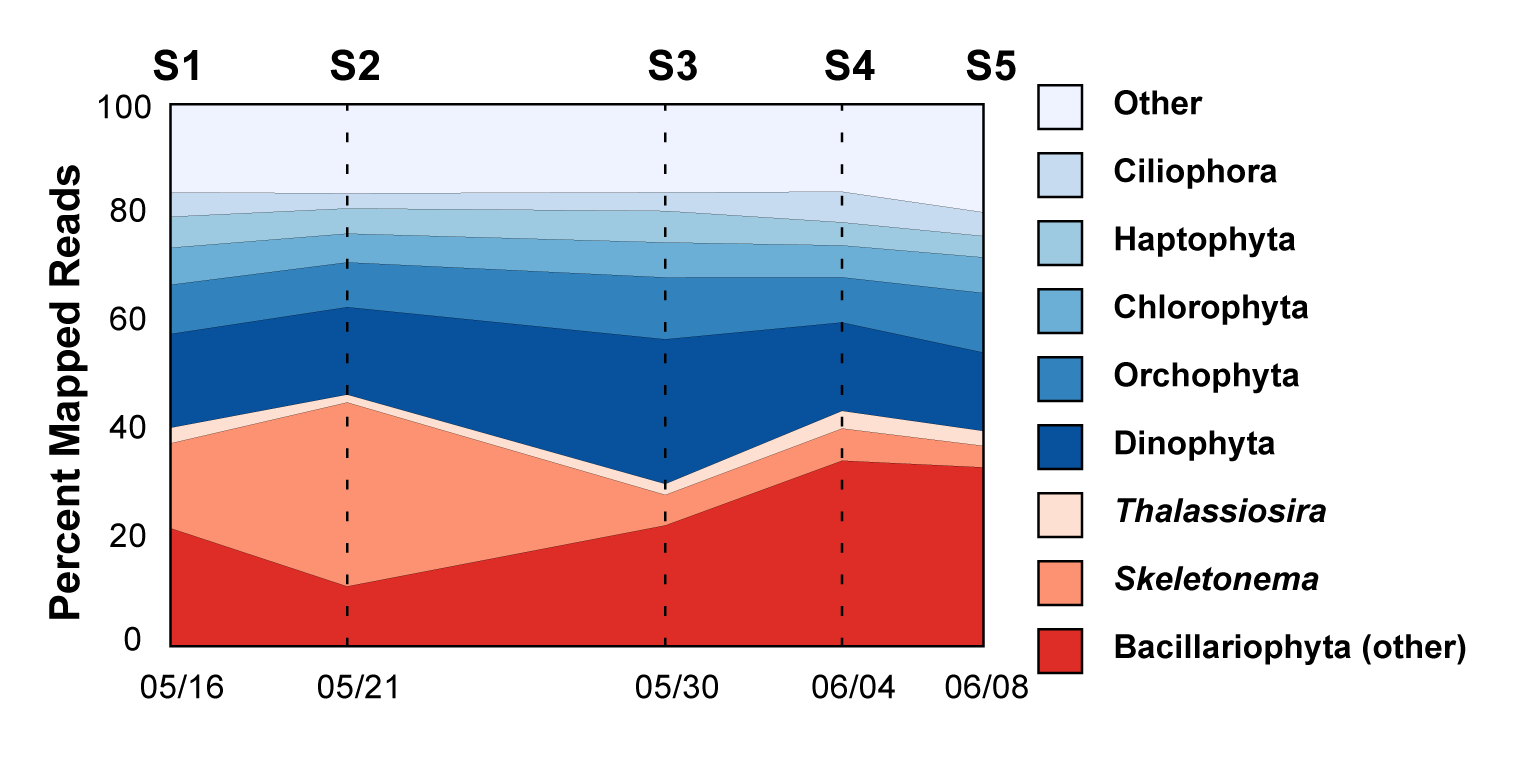
\includegraphics[width=1\textwidth]{Images/C3_Figure1_StackPlot.png}
    \caption[Taxonomic classification of reads across five field samples]{Taxonomic classification of RNA-seq paired end reads across the five field samples. Classification was determined by mapping to a database comprised of all publicly available transcriptomes through the Marine Microbial Eukaryotic Transcriptome Project (MMETSP) as of March 17, 2014.}
  \label{fig:c3f1}
\end{figure}

\subsection{Temporal plasticity in expressed metabolic capacity} 
Metatranscriptome short reads were mapped to transcriptomes that had been annotated with Kyoto Encyclopedia of Genes and Genomes (KEGG) orthology (KO) (\ref{DS31}), allowing the expression of KO gene families within a KEGG module (higher-level groupings of KO gene families into pathway or functional classifications) to be examined over time. Normalizing the expression of KEGG modules to the total KEGG annotated reads for each organism across time yielded the Quantitative Metabolic Fingerprint (QMF), which highlighted differences between the two species and differences across time for each species (\cref{fig:c3f2}). A comparison of the total number of annotated genes falling into each of the KEGG modules revealed a close to one-to-one linear relationship (slope of 1.0948, $R^{2}=0.9123$) (\cref{fig:a3f2}), indicating that the observed differences are not an artifact of gene distribution between organisms. The QMFs of the two organisms were distinct and there were significant shifts in the QMF of each species over time reflecting considerable plasticity in the expressed metabolic capacity (\cref{fig:a3f3}). Central carbohydrate metabolism, carbon fixation, and other carbohydrate metabolism were some of the most highly expressed KEGG modules in the field for both \textit{Skeletonema} spp. and \textit{T. rotula}, though higher for \textit{Skeletonema} spp., where expression of these pathways peaked during S4 representing over 84\% of mapped KEGG reads (\cref{fig:c3f2}). The largest global shift in KEGG module expression was seen in \textit{Skeletonema} spp. on S2 (\cref{fig:a3f3}), when its density peaked at 11,520,000 cells L$^{-1}$. The S2 time point for \textit{Skeletonema} spp. had increased QMF signals in ATP synthesis, proteasome, and ubiquitin systems and decreased QMF signals in photosynthesis and carbon metabolism relative to other time points. For example, reads mapping in photosynthesis dropped by over an order of magnitude from 0.3-2.2\% of annotated transcripts in S1, S3-5 to 0.03\% during S2 (\cref{fig:c3f2}). The temporal plasticity of transcript allocation to different aspects of metabolism for both species was striking and likely reflects the dynamic environment which they inhabit: an estuary, where the geochemistry is highly variable \citep{Nixon1995}.\par
Temporal plasticity in the KEGG module expression patterns, including a shift away from the expression of carbon fixation and photosynthesis suggests that the elevated \textit{Skeletonema} spp. cell numbers observed in S2 may have been after this diatom reached peak bloom biomass. A significant proportion of the KEGG modules expressed were classified as ribosomes (5-45\% for \textit{Skeletonema} spp. and 5-9\% for \textit{T. rotula}). \citet{Gifford2013} suggested that ribosomal protein expression correlates with growth rate. Applying this principle to these eukaryotic data suggests the growth rates for both \textit{Skeletonema} spp. and \textit{T. rotula} fluctuated, with peaks in growth rate occurring during S1 and S3 for \textit{Skeletonema} spp.. This pattern for \textit{Skeletonema} spp. did not track with the relative abundance of the organism, which peaked in the S2 sample, again suggesting that this sample was taken during the bloom decline. These growth dynamics cannot be fully resolved without a more detailed sample set.\par

% Figure 2
\begin{figure}[p!]
  \centerline{ 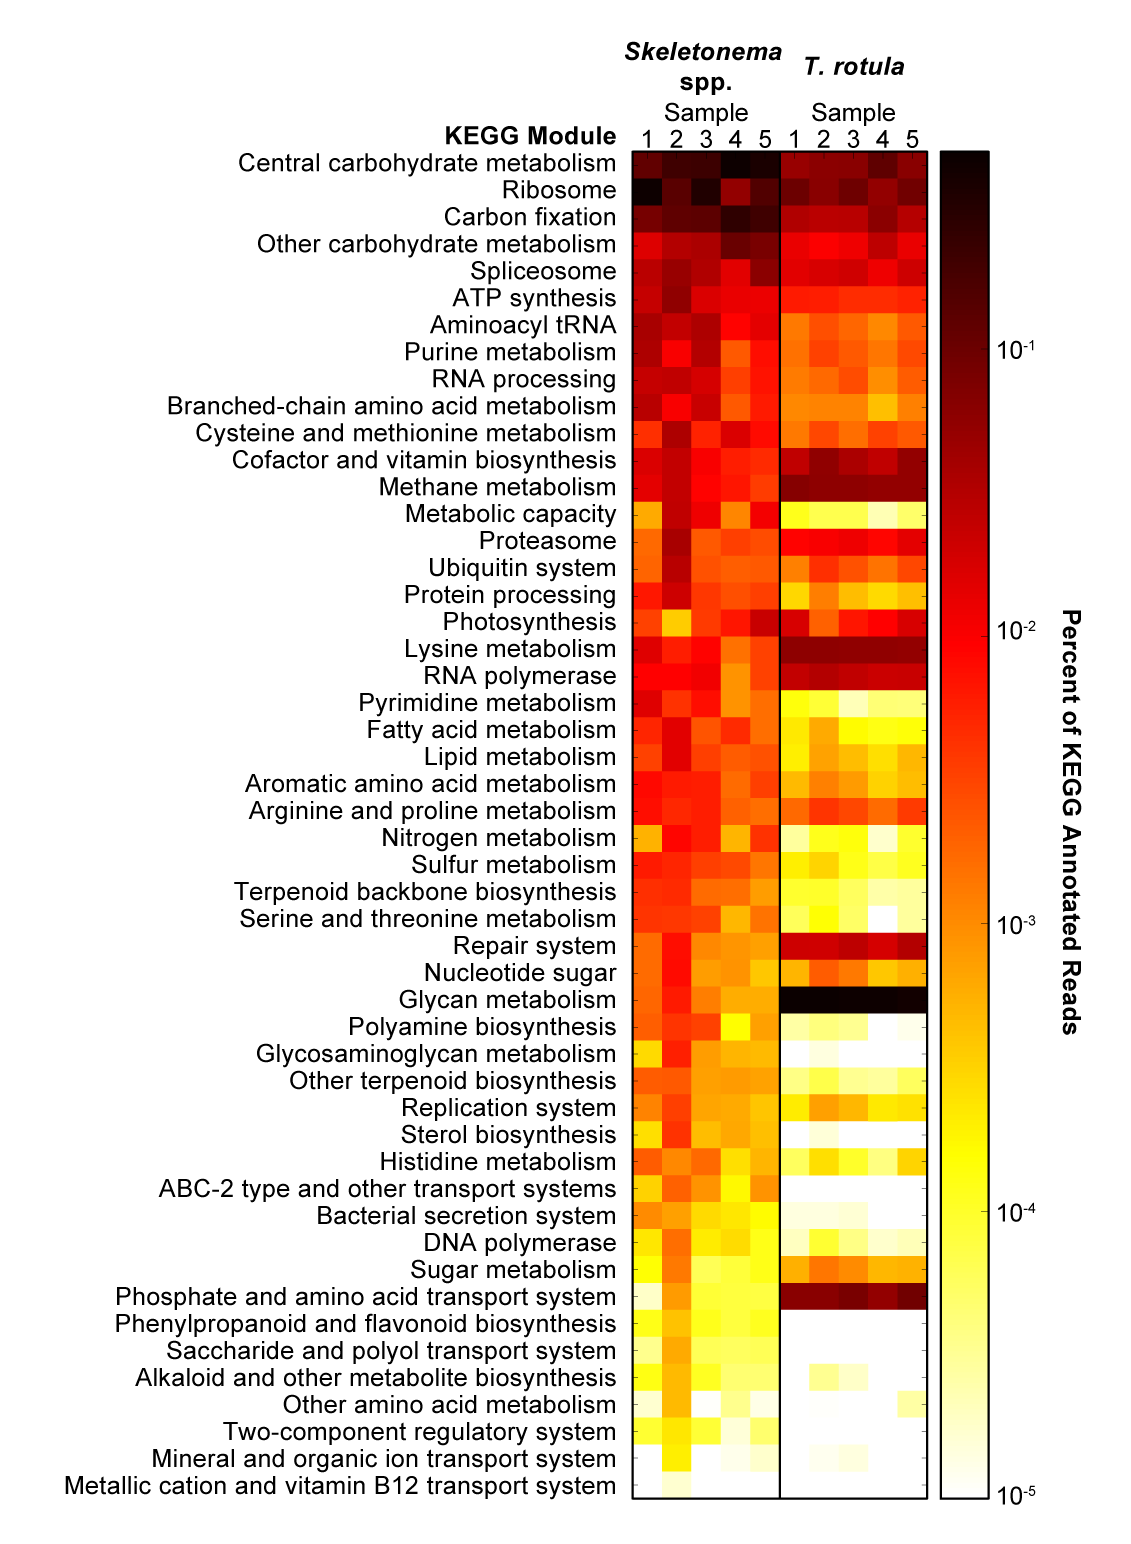
\includegraphics[width=1\textwidth]{Images/C3_Figure2_Heatmap_Hot.png}}
    \caption[Quantitative metabolic fingerprint across Narragansett Bay \textit{in situ} samples]{Quantitative metabolic fingerprint (QMF) depicting the relative expression of KEGG modules for \textit{Skeletonema} spp. and \textit{T. rotula} in Narragansett Bay across the five sampling time points (S1-S5). Color indicates the proportion of total reads mapping to each KEGG module relative to all KEGG annotated reads.}
  \label{fig:c3f2}
\end{figure}

\textit{Skeletonema} spp., the dominant diatom during the study period (\cref{fig:c3f1}), had a higher proportion of transcripts related to growth relative to \textit{T. rotula}, such as those encoding aspects of carbon metabolism, N metabolism, sulfur metabolism, and lipid metabolism (\cref{fig:c3f2}). Conversely, several KEGG modules were more highly expressed in \textit{T. rotula} compared to \textit{Skeletonema} spp., particularly those for glycan metabolism, phosphate and amino acid transport systems, and repair system modules (\cref{fig:c3f2}). The majority of highly expressed KO modules (e.g. N metabolism) were based on moderate to high expression across several KO gene families, but, in some cases, the differences in expression at the module level were due to differences in the expression of a single KO gene family within the KEGG module. For example, the driver of the difference in the expression of glycan metabolism, which represented upwards of 41\% of all KEGG annotated reads for \textit{T. rotula} compared to less than 0.6\% for \textit{Skeletonema} spp., was primarily associated with the high expression of a putative UDP-N-acetylglucosamine-dolichyl-phosphate N-acetylglucosaminephosphotransferase (K01001). This was identified as a silaffin-like response gene associated with silica polymerization \citep{Shrestha2012}. Differences in silica metabolism may in part drive how the fundamental niche is segregated between these two diatoms. Taken together, the contrast in QMF between the two diatoms underscores the fundamental differences in expressed metabolic capacity that are present in these two co-occurring diatoms and highlights traits of a successful competitor (e.g. high expression of carbon metabolism).\par

\subsection{Species-specific resource utilization underpins physiological ecology}
KO gene families related to N and P metabolism were examined in the field samples to identify species-specific patterns in resource utilization. \textit{Skeletonema} spp. and \textit{T. rotula} both possess and express core pathways of N and P metabolism (such as the ornithine-urea cycle) (\cref{fig:c3f3}). Expression of these individual KO gene families was temporally variable, as was observed with the expression of KEGG Modules, but related enzymes in a pathway exhibited a coordinated response (\cref{fig:c3f3}). For example, the nitrate transporter (K02575), nitrate reductase (K10534), and nitrite reductase (K00366), in \textit{Skeletonema} spp. all had peak expression in S2 (\cref{fig:c3f3}). \textit{Skeletonema} spp. and \textit{T. rotula} share pathway homologs, including the same suite of N transporters (ammonium: AMT, nitrate: NRT, amino acid: AAPJ), but these genes often had disparate patterns of expression between the two species (\cref{fig:c3f3}). \textit{Skeletonema} spp., the more abundant diatom, had high expression of KO gene families associated with the acquisition of nitrate and ammonia that were particularly amplified during the S2 bloom event. \textit{T. rotula} had low expression of both of those transporters but high expression of a general amino acid transporter (\cref{fig:c3f3}). Amino acid transport \citep{North1972} and nitrate transport \citep{Serra1978} has previously been found to inversely correlate with intracellular nitrate concentration in the cell or the presence of ammonia in the media. Yet, here, two closely related diatoms, existing in the same parcel of water and the same nutrient environment, are expressing genes to access different pools of dissolved N. Similar to nitrate transport, there was high expression of nitrate/ nitrite reductase KO gene families in \textit{Skeletonema} spp., whereas \textit{T. rotula} appears to possess a different N reduction metabolism. This is observed in a KO gene family that is absent from the reference transcriptome of \textit{Skeletonema} spp.: hydroxylamine reductase (\cref{fig:c3f3}). This gene has been found in the genomes of both \textit{T. pseudonana} and \textit{P. tricornutum}, and is thought to have been acquired via lateral transfer from bacteria \citep{Bowler2008}. The enzyme may potentially aid redox balancing and electron cycling from nitrate reduction \citep{Allen2008}. While the absence of this gene in \textit{Skeletonema} spp., has not been definitively shown, the marked high expression of this gene in \textit{T. rotula} suggests that this gene product represents a potential point of segregation in the metabolic capacity of these two species. Together, these data suggest that these species have disparate strategies for acquiring N and this may in part drive the relative success of \textit{Skeletonema} spp. over the sample period.\par

%Figure 3

\begin{figure}[p!]
  \centering
    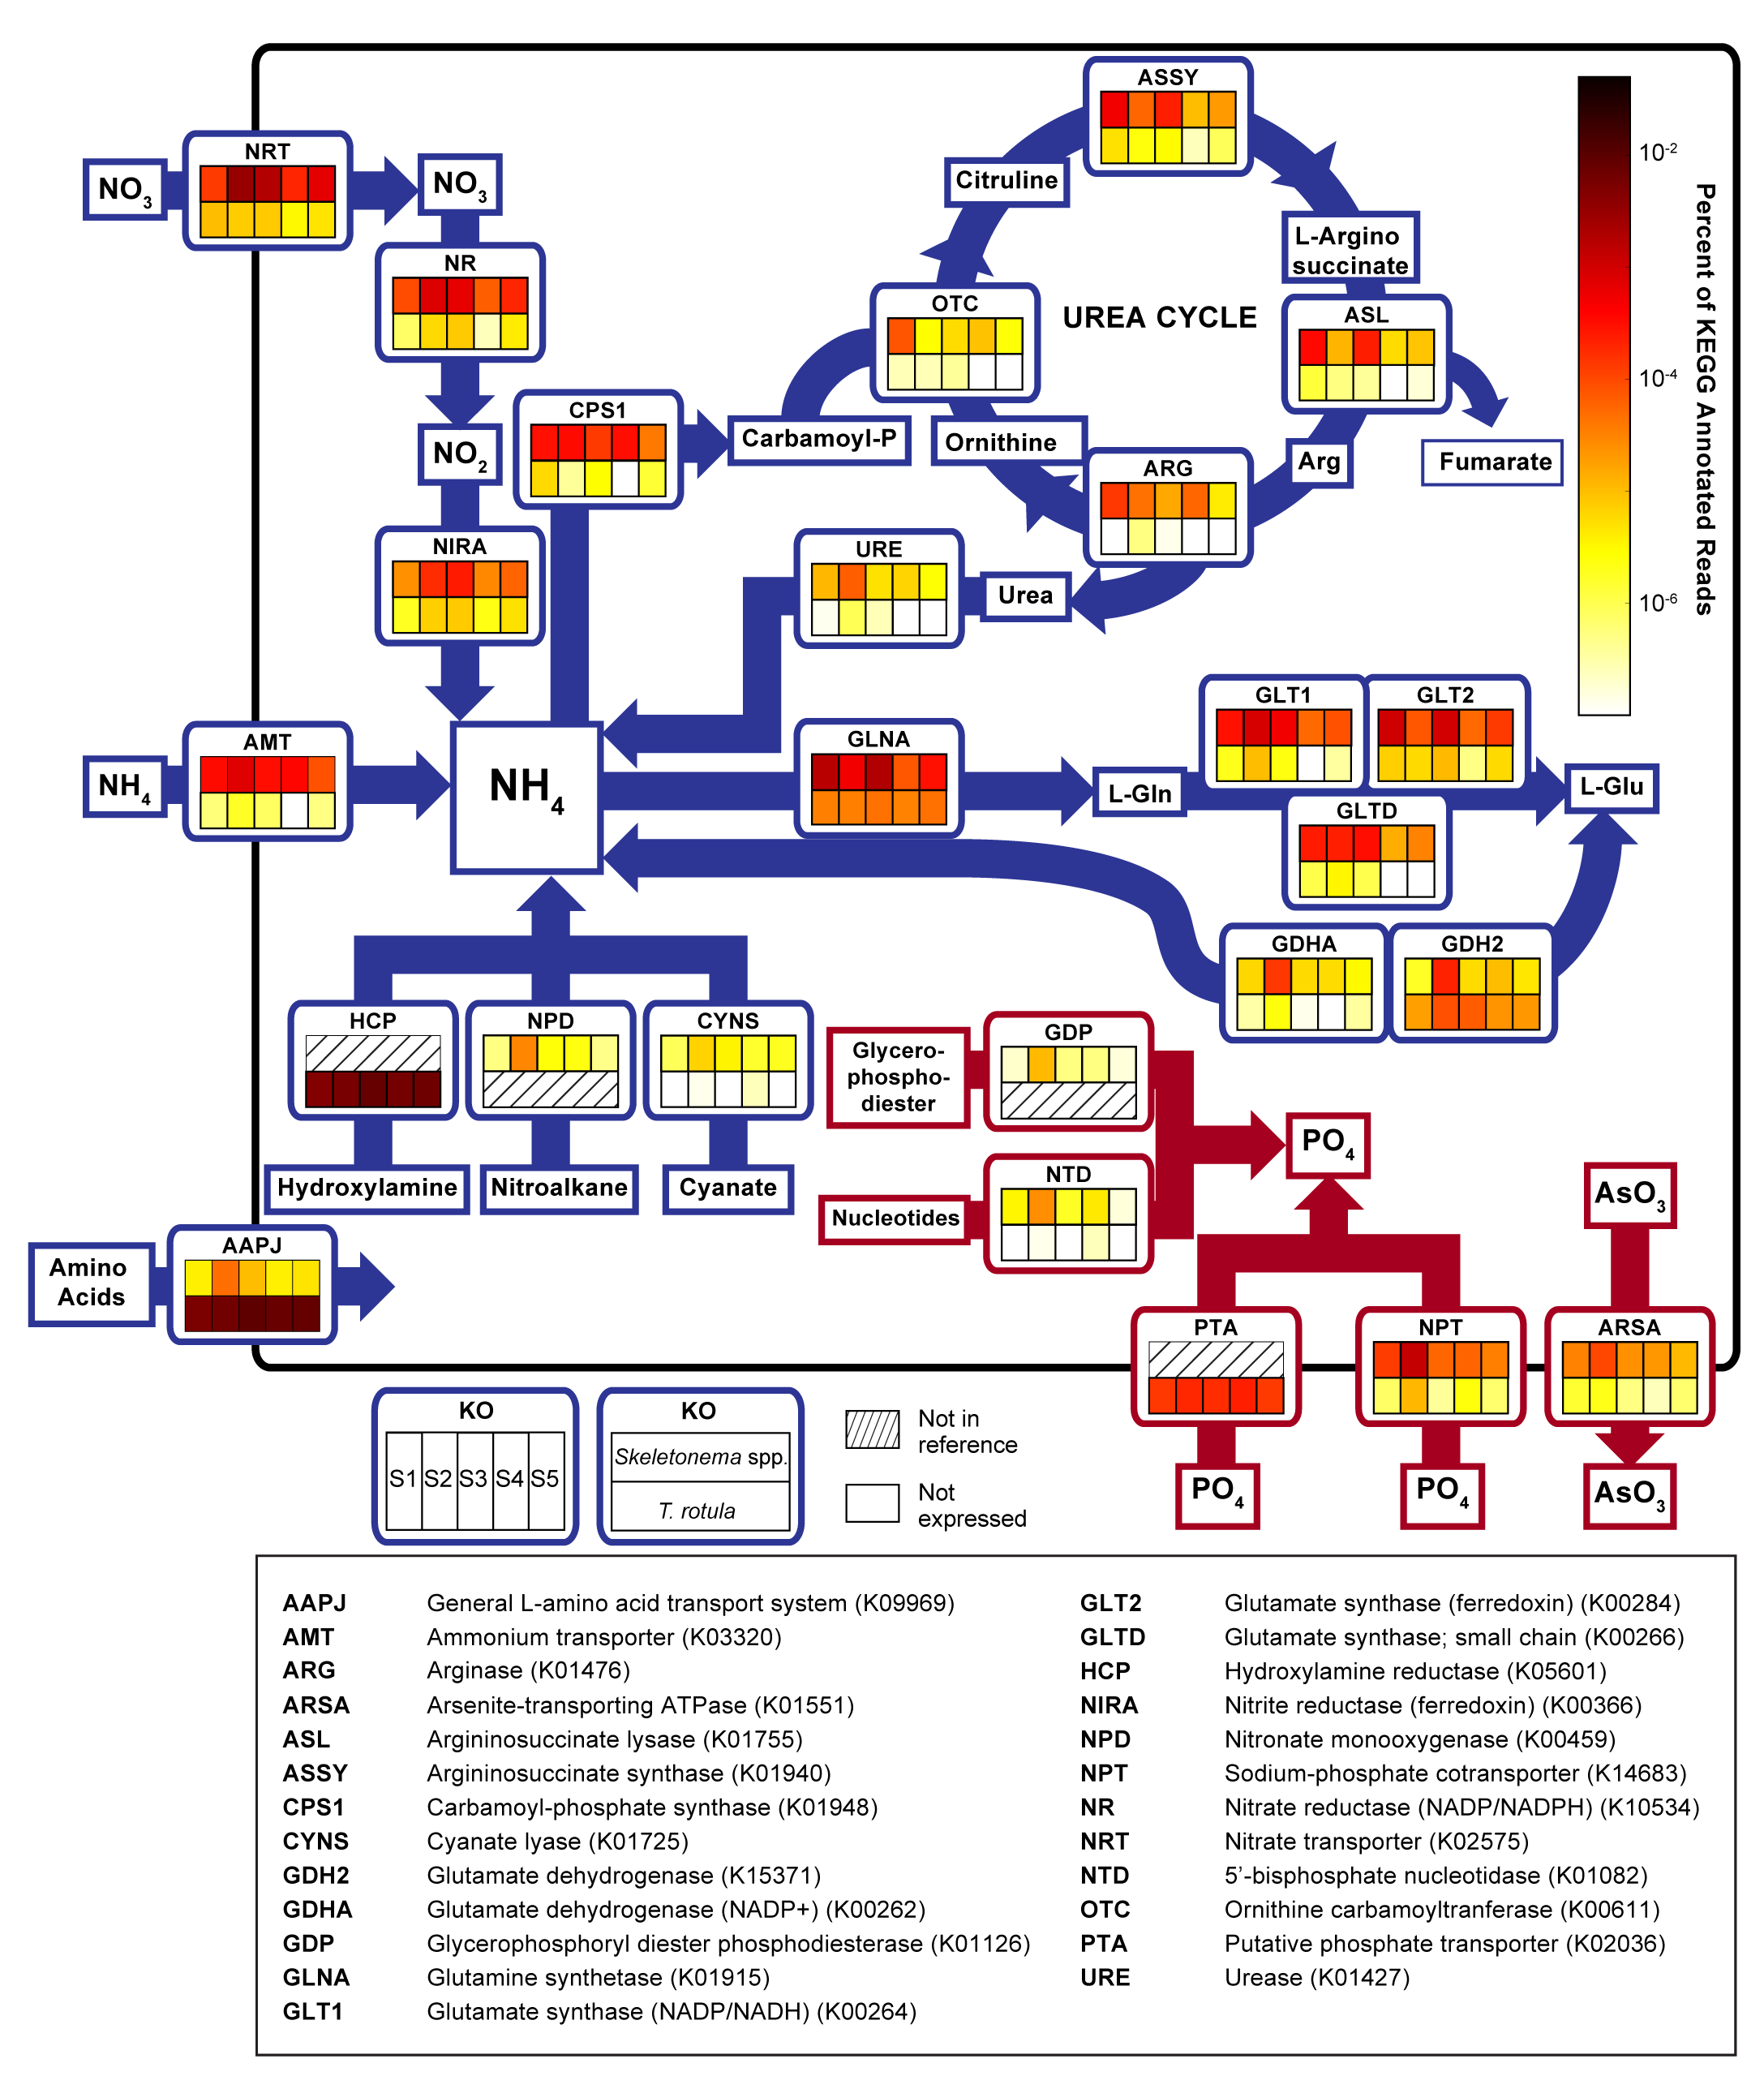
\includegraphics[width=1\textwidth]{Images/C3_Figure3_CellHeatmap_Hot.png}
    \caption[Modulation of nitrogen and phosphorus pathways in the field]{Schematic cell model depicting the relative expression of KO gene families associated with nitrogen (N) and phosphorus (P) metabolic pathways for \textit{Skeletonema} spp. and \textit{T. rotula} in Narragansett Bay across the five sampling time points (S1-S5). Color indicates the proportion of total reads mapping to each KEGG module relative to all KEGG annotated reads.}

  \label{fig:c3f3}
\end{figure}



While N has been observed to be a primary nutritional driver in Narragansett Bay \citep{Nixon1995,Smayda1974,Sakshaug1977}, P may also drive the dynamics of these two diatoms. \textit{Skeletonema} spp. shows elevated expression of a sodium phosphate cotransporter (NPT), again with peak expression during S2 (bloom). \textit{T. rotula} does express the NPT as highly, but by comparison has a much higher transcript count for a putative P transporter (PTA), that is not detected in \textit{Skeletonema} spp. (\cref{fig:c3f3}). These transporters may have different kinetic properties that allow the two species to diverge in their PO$_4$ uptake strategies.  Genes associated with the scavenging of P from organic molecules, such as glycerophosphoryl diester phosphodiesterase (GDP), also suggest differences in expressed metabolic capacity between the two species. GDP may be associated with exogenous metabolism of dissolved organic P (DOP) or internally in the cleaving of P from lipids \citep{VanMooy2009, Dyhrman2012}. The expression of GDP by \textit{Skeletonema} spp., with peak around S2, and apparent absence of this transcript in \textit{T. rotula} suggests \textit{Skeletonema} spp. may be accessing a pool of DOP that is not being utilized by \textit{T. rotula}. In \textit{T. pseudonana}, related transcripts are tightly linked to concomitant changes in the proteome and biochemical activities \citep{Dyhrman2012}.  If these transcriptional patterns are linked to similar changes in activities, then these insights suggest that there is a fundamental difference in the metabolic capacity being expressed in the same environment by the two diatoms.  \textit{Skeletonema} spp. is both actively taking up PO$_4$ and hydrolyzing organic sources, where as \textit{T. rotula} is not hydrolyzing DOP and is taking up inorganic PO$_4$ by a different mechanism.  In summary, these data suggest that these two diatoms have unique metabolic capacity for the utilization of specific forms of N and P. Such disparate resource utilization potential could be a niche-defining feature that underpins diatom diversity as well as the ``winner-loser'' dynamic observed here with the differences in cell abundance between the species.\par
\subsection{Identification and modulation of resource responsive genes \textit{in situ} highlights species-specific differences}
To identify and quantitatively track resource responsive (RR) genes \textit{in situ}, incubation experiments were used to examine species-specific transcriptional responses to shifts in N:P ratios. Comparing the expression patterns between like nutrient treatments (+N versus -N and +P versus -P) for each of the organisms enabled the statistical identification of a suite of RR genes \citep{Wu2010} and stable reference genes \citep{Alexander2012}. RR gene counts were normalized to the stable reference genes (\cref{fig:a3f4}) resulting in stable gene normalized counts ($SGNC$). Calculation of a $SGNC$ is similar in concept to reference gene normalization done in qRT-PCR \citep{Bustin2000} or metatranscriptome studies of prokaryotes \citep{McCarren2010}, with the added value of not having to rely on reference genes from model diatoms.\par
Of the transcripts expressed at greater than 2 tags per million (TPM) for at least one treatment, 24.5\% and 17.9\% were identified as RR by being significantly up or down-regulated between N or P treatments for \textit{Skeletonema} spp. and \textit{T. rotula}, respectively (\ref{DS32}, \cref{tab:a3t3}). As is common with phytoplankton studies \citep{Marchetti2012a}, the majority of the RR genes do not have a KEGG annotation (\cref{fig:a3f4}A). The portion of the RR gene set annotated with KEGG ontology for \textit{Skeletonema} spp. and \textit{T. rotula} revealed that, relative to the full KEGG profile, genes comprising genetic information processing associated with replication (encompassing ribosomes, nucleotide replication and processing) were underrepresented for both organisms in the RR set (\cref{fig:a3f5}). By contrast, the RR sets were enriched for energy, carbohydrate, and lipid metabolism, which encompass pathways known to be associated with the metabolism of N and P (\cref{fig:c3f4}A, \cref{fig:a3f5}). Specific genes in this set included, but were not limited to, those associated with N assimilation (e.g. glutamate dehydrogenase, glutamine synthase, nitrate reductase), DON utilization (e.g. urease, aminopeptidase, amino-acid transport system), P scavenging (e.g. phosphate transporter, sodium phosphate cotransporter) and DOP utilization (e.g. phosphatases) (\ref{DS32}). A number of these genes have been shown to be N or P responsive in transcriptional studies with cultures of the diatom \textit{T. pseudonona} \citep{Dyhrman2012, Bender2014}, and transporters, and enzymes for the processing of organic N or P, as observed here, are well known to be resource responsive in many phytoplankton \citep{Dyhrman2012, Wurch2011, Dyhrman2006, Bruhn2010}. Overall, these genes demonstrated patterns of regulation \textit{in situ} (\cref{fig:c3f4}B, \cref{fig:a3f6}) similar to what has been observed in culture \citep{Dyhrman2012, Bender2014}. In the incubations, the sodium-phosphate cotransporter (NPT) was significantly up-regulated in the -P treatment for both species (\cref{fig:c3f4}B), which is consistent with P regulation of a \textit{T. pseudonana} NPT homolog (Thaps\_24435) observed in culture experiments (56). Nitrate reductase, which has been shown to be regulated by N in \textit{T. pseudonana} (Thaps\_25299) \citep{Bender2012}, was up-regulated in -N for \textit{T. rotula}, but not \textit{Skeletonema} spp. (\cref{fig:a3f6}). In fact, members of this large gene family (\cref{fig:a3f7}) showed disparate regulation in both species (\cref{fig:a3f6}).  These data demonstrate that the use of nutrient amendments is robust for normalizing and identifying N and P responsive genes in the field that are consistent with known signals, but also point to the value of \textit{in situ} analyses, as application of a priori knowledge about regulation from model diatoms could lead to misinterpretations.\par

% Figure 4


\begin{figure}[p!]
  \centering
    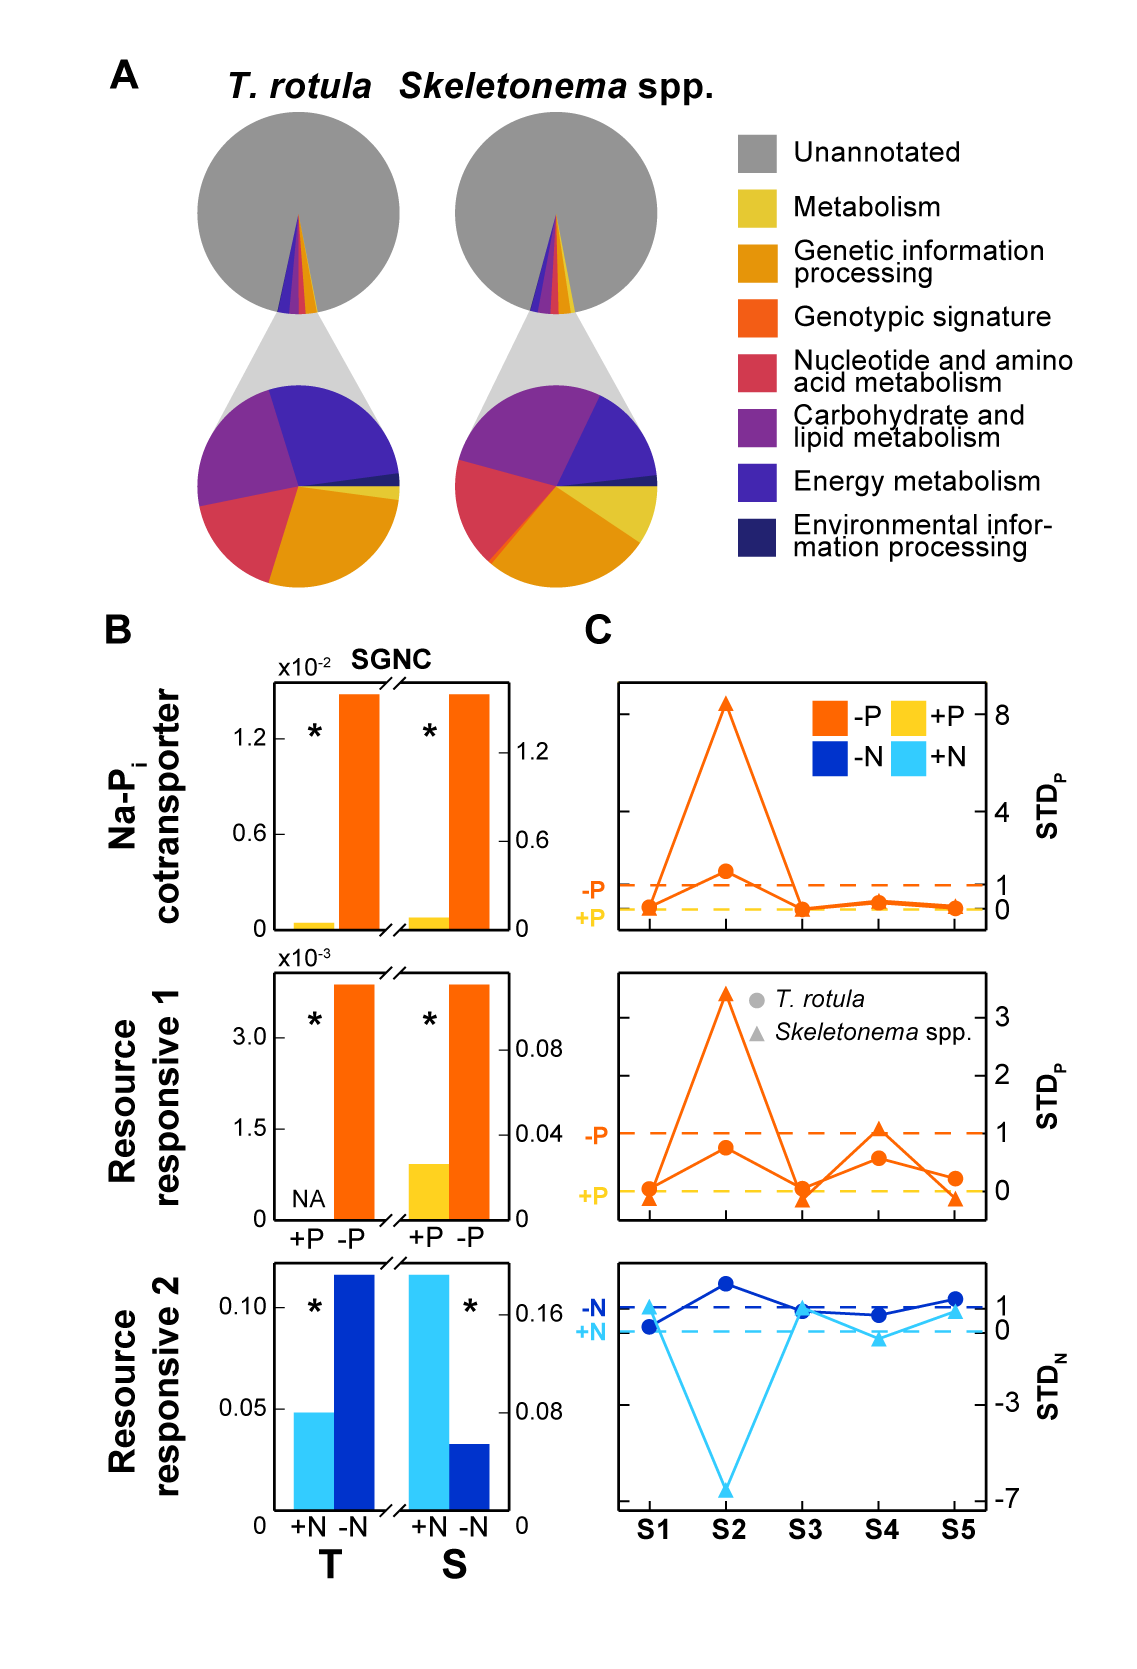
\includegraphics[width=.65\textwidth]{Images/C3_Figure4_BarLinePlots.png}
    \caption[Functional composition of resource-responsive gene set]{Functional composition of the resource-responsive (RR) gene sets for \textit{T. rotula} and \textit{Skeletonema} spp. (A), the relative expression in the incubation samples (B) and standardized transcriptional differentiation (STD) scores (C) for a known P-responsive gene, sodium-phosphate cotransporter, and two novel RR gene families. (A) The RR gene sets were identified through cross comparison of like-nutrient incubations (i.e. +N vs. -N and +P vs. -P), using ASC (fold change = 2, post-$p > 0.95$) (57). The relative functional categorization of the RR gene set for \textit{T. rotula} and \textit{Skeletonema} spp. based on KEGG ontology as assigned by KAAS is depicted at the module-level relative to the portion unannotated with KEGG. (B) Expression pattern in stable gene normalized counts ($SGNC$) of the genes from the associated gene cluster from \textit{T. rotula} (T) and \textit{Skeletonema} spp. (S) plotted in related incubations (i.e. novel P-responsive shows expression from +P and -P incubations). Asterisk indicates significance between pair-wise comparisons (fold change = 2, post-$p > 0.95$) (57). (C) $STD$ scores plotted across the five sample points showing $STD_P$ for the P-significant genes and $STD_N$ for the N-significant genes. Dashed horizontal lines at 0 and 1 indicate the +P/+N and -P/-N for corresponding significant genes.} 
  \label{fig:c3f4}
\end{figure}

Of the RR gene sets for \textit{Skeletonema} spp. and \textit{T. rotula}, only 17.7 and 12.7\% of the genes, respectively, were annotated with KEGG ontology (\cref{fig:c3f4}A). Identifying differentially regulated genes \textit{in situ} through experimental manipulations allowed the expression patterns of genes to be tracked even when their function was unknown. As an example, two RR gene families were identified with homologs in \textit{Skeletonema} spp. and \textit{T. rotula} (\cref{fig:c3f4}B, \cref{fig:a3f7}). RR1 was up-regulated in -P compared to +P for both species (\cref{fig:c3f4}B). Homologs from RR1 were also identified in other diatom genomes (Fracy\_268075, Phatr\_19661, Psemu\_246578, Psemu\_319824, Thaps\_32459) (\cref{fig:a3f7}). Annotations for these genes were limited, though Fracy\_268075 was identified as possibly involved in intracellular trafficking, secretion, or vesicular transport, suggesting these proteins may be involved in poly-P metabolism \citep{Ogawa2000}. RR2 demonstrated significantly different patterns of regulation in the two species: up-regulated in -N compared to +N for \textit{T. rotula} but down-regulated in -N compared to +N for \textit{Skeletonema} spp. (\cref{fig:c3f4}B). A homolog from RR2 was identified in \textit{T. pseudonana} (Thaps\_22648) (\cref{fig:a3f7}) and was poorly characterized, with the best BLAST hit to a human dentin sialophosphoprotein. This suggests RR2 could be associated with biomineralization.\par
To enable cross-comparison of the RR genes between species, their expression was put into a greater metabolic context by proportionalizing the expression in the field to the transcriptional range observed in the incubations with extremes in the N:P ratio. This technique is similar in concept to targeted assays using qRT-PCR to compare expression patterns between species in culture \citep{Kang2009}. Briefly, the $SGNC$ of a gene in the field was bounded by the $SGNC$ from each of the nutrient treatments to yield the standardized transcriptional differentiation score for both N ($STD_N$) and P ($STD_P$) (\cref{fig:c3f4}C). The $STD$ score was used to directly compare expression relative to its maximum and minimum capacity where values of $STD \geq 1$ indicate signals are similar to the deplete condition, and values of $STD \leq 0$ indicate similarity to the replete condition. The $STD_N$ and $STD_P$ were plotted for genes from the NPT and the two highlighted RR gene families, over the time-series (\cref{fig:c3f4}C). The NPT for both \textit{Skeletonema} spp. and \textit{T. rotula} showed elevated expression during S2. RR1, which was also identified as significantly expressed in -P compared to +P, also showed elevation during S2 (the bloom day). The expression of RR1, however, was also elevated on S4 for both diatoms, which was not seen for the NPT. However, $STD_P >1$ for \textit{Skeletonema} spp. indicating a far more P deficient response in \textit{Skeletonema} spp. compared to \textit{T. rotula}, which never demonstrated P-sensitive expression in the field comparable to that observed in the -P incubations (\cref{fig:c3f4}C). RR2 showed different patterns of expression across time for both species. Most interestingly, perhaps, was the low $STD_N$ score for \textit{Skeletonema} spp. during its bloom period indicating that the RR2 expression was more similar to the +N treatment, whereas the $STD_N$ for \textit{T. rotula} was greater than one suggesting that expression was more similar to the -N treatment (\cref{fig:c3f4}C). These three, targeted examples suggest that during the large bloom of \textit{Skeletonema} spp., \textit{Skeletonema} spp. was expressing genes in pattern more similar to the -P and +N treatments, while the expression of \textit{T. rotula} was more similar only to the -N treatment. Notably, these are orthogonal patterns associated with the same environment. \par
% Figure 5
\begin{figure}[h!]
  \centering
    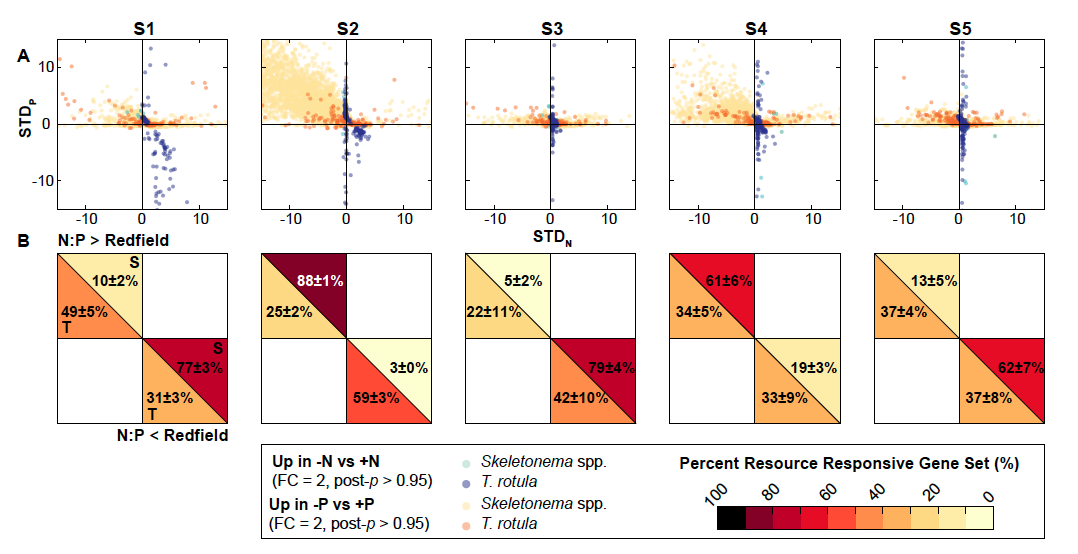
\includegraphics[width=1\textwidth]{Images/C3_Figure5_Quadrants.png}
    \caption[Evolution of resource-responsive (RR) gene partitioning over time in Narragansett Bay]{Evolution of resource-responsive (RR) gene partitioning over time in Narragansett Bay for \textit{T. rotula} and \textit{Skeletonema} spp.. (A) The stable gene normalized field signal for each gene identified as significantly (2-fold change, post-p > 0.95) up-regulated in -P vs. +P for \textit{Skeletonema} spp. (yellow) and \textit{T. rotula} (orange) and in -N vs. +N for \textit{Skeletonema} spp. (cyan) and \textit{T. rotula} (dark blue) were proportionalized relative to the expression for those genes in nutrient incubations, yielding the $STD_N$ and $STD_P$ for each gene. These data are plotted for Sample 1 through Sample 5. (B) The proportion of identified RR genes falling into the N:P > Redfield and N:P < Redfield quadrants for \textit{T. rotula} (T) and \textit{Skeletonema} spp. (S).}

  \label{fig:c3f5}
\end{figure}

The $STD_N$ and $STD_P$ for all of the RR genes were calculated (\ref{DS32}) to expand upon the single gene analyses above. The RR genes were plotted based on the $STD_N : STD_P$ (\cref{fig:a3f8}) to examine how similar the pattern was to the incubation N:P ratio (\cref{fig:c3f5}A, \cref{fig:a3f9}). Redfield regimes have historically been used to characterize different aquatic environments based on the ratio of nutrient resources required for growth. For example, a Redfield ratio of N:P = 16, here called ``Redfield'', would predict neither P nor N limitation. As expected, RR genes identified as N-regulated genes fall primarily into the N:P < Redfield quadrant and P-regulated genes fall primarily into the N:P > Redfield quadrant for both \textit{Skeletonema} spp. and \textit{T. rotula} (\cref{fig:c3f5}A). Observing patterns in distribution of these genes across time, S2 stands out amongst the time points, where a significant (88\%) proportion of the P-regulated genes from \textit{Skeletonema} spp. move far into the N:P > Redfield quadrant (\cref{fig:c3f5}A). This N:P > Redfield physiology is consistent with the single gene analyses (\cref{fig:c3f4}C) and suggests P availability may have constrained \textit{Skeletonema} spp. populations during the bloom sample (S2). Conversely, a large proportion (59\%) of the N-regulated genes in \textit{T. rotula} move into the N:P < Redfield quadrant (\cref{fig:c3f5}A) consistent with the divergent responsiveness of RR2 observed for \textit{T. rotula} compared to \textit{Skeletonema} spp. (\cref{fig:c3f4}C). In fact, with the exception of S4 and S5 where \textit{T. rotula} had even distribution between the N:P > Redfield and N:P < Redfield quadrants, the two species always showed statistically significant (Tukey HSD analysis ($p<0.05$)) orthogonal responses in the distribution of the RR gene set across the two quadrants (\cref{fig:c3f5}B, \cref{fig:a3f10}). These patterns combined with the temporal variability in gene expression patterns indicate a finely tuned response to the environment, which is distinctive for each diatom species. Although there are many potential controls on diatom dynamics in Narragansett Bay, including top-down processes like predation \citep{Martin1970, Lawerence2012}, these patterns of resource responsive gene expression suggest the presence of bottom-up nutrient control on diatom population dynamics in Narragansett Bay.\par

This work addresses fundamental knowledge gaps in how phytoplankton species are able to co-occur while they compete for the same basic resources. Co-occurring diatoms appear to have different functional capabilities in N and P metabolism, and this metabolic potential is modulated in field populations in a distinctive way for each diatom. These findings suggest that differential resource partitioning is occurring between these two diatoms \textit{in situ}. Such resource partitioning could facilitate the vast diversity of the phytoplankton and the structure, function, and productivity of aquatic ecosystems. In culture studies, resource-related transcriptional changes have been shown to be tightly choreographed with changes in proteins, activities, and biochemical pools (56, 62, 69). If further work were able to similarly link the transcriptional patterns observed here with changes in enzymatic activities or uptake rates, then shifts in the RR gene sets may reflect aspects of the realized niche and how it differs between these two species. These detailed, \textit{in situ} transcriptional comparisons would not have been possible without proportionalization to metabolic capacity (STD), which provides a quantitative means to directly compare transcriptional patterns between species. This approach could be applied to other systems, organisms, or environmental parameters to identify responsive genes and proportionalize their expression, with the aim of answering similar questions about how co-occurring species adjust their cellular physiology to partition their niche space.\par




\chapter{Functional group-specific traits drive phytoplankton dynamics in the oligotrophic ocean}
\label{chap:4}
\raggedbottom

%\begin{singlespace}
%Harriet Alexander$^{1,2}$, M\'{o}nica Rouco$^3$, Sheean T. Haley$^3$, Samuel T. Wilson$^4$, David M. Karl$^4$, Sonya T. Dyhrman$^{3}$\\
%\\
%$^{1}$ MIT-WHOI Joint Program in Oceanography/Applied Ocean Science and Engineering, Cambridge, MA 02139, USA\\
%$^2$ Biology Department, Woods Hole Oceanographic Institution, Woods Hole, MA 02543, USA\\
%$^3$ Department of Earth and Environmental Sciences Lamont-Doherty Earth Observatory, Columbia University, Palisades, NY 10964\\
%$^4$ Daniel K. Inouye Center for Microbial Oceanography: Research and Education, Department of Oceanography, University of Hawaii, Honolulu, HI 96822, USA\\
%\\
{\let\thefootnote\relax\footnotetext{This chapter was originally published as Alexander, H., R\'{o}uco, M., Haley, S.T., Wilson, S.T., Karl, D.M., and Dyhrman, S.T. (2015). \href{http://www.pnas.org/content/112/44/E5972.full}{Functional group-specific traits drive phytoplankton dynamics in the oligotrophic ocean.} \emph{Proc. Natl. Acad. Sci. U. S. A.} 112:44, E5972-E5979.}}
{\let\thefootnote\relax\footnotetext{H.A. and S.T.D. designed research; H.A., M.R., S.T.H., S.T.W., and S.T.D. performed research; H.A., D.M.K., and S.T.D. analyzed data; H.A. and S.T.D. wrote the paper; and M.R., S.T.H., S.T.W., and D.M.K. contributed to the writing of the paper.}}
{\let\thefootnote\relax\footnotetext{The supplemental figures, tables, and data sheets for this chapter can be found in \cref{sec:app4}.}}



%\end{singlespace}
\clearpage

\section{Abstract} 
A diverse microbial assemblage in the ocean is responsible for nearly half of global primary production. It has been hypothesized and experimentally demonstrated that nutrient loading can stimulate blooms of large eukaryotic phytoplankton in oligotrophic systems. Although central to better balancing biogeochemical models, knowledge of the metabolic traits that govern the dynamics of these bloom-forming phytoplankton is limited. We employed eukaryotic metatranscriptomic techniques to identify the metabolic basis of functional group-specific traits that may drive the shift between net heterotrophy and autotrophy in the oligotrophic ocean. Replicated blooms were simulated by deep seawater (DSW) addition to mimic nutrient loading in the North Pacific Subtropical Gyre and the transcriptional responses of phytoplankton functional groups were assayed. Responses of the diatom, haptophyte, and dinoflagellate functional groups in simulated blooms were unique, with diatoms and haptophytes significantly (95\% confidence) shifting their quantitative metabolic fingerprint from the \textit{in situ} condition, while dinoflagellates showed little response. Significantly differentially abundant genes identified the importance of co-limitation by nutrients, metals, and vitamins in eukaryotic phytoplankton metabolism and bloom formation in this system. The variable transcript allocation ratio, used to quantify transcript reallocation following DSW amendment, differed for diatoms and haptophytes, reflecting the long-standing paradigm of phytoplankton r- and K-type growth strategies. While the underlying metabolic potential of the large eukaryotic phytoplankton was consistently present, the lack of a bloom during the study period suggests a crucial dependence on physical and biogeochemical forcing, which are susceptible to alteration with changing climate. 
 
\section{Introduction}
It has been postulated that the net oxygen state of oligotrophic systems is controlled by irregular blooms of large eukaryotic phytoplankton \citep{Karl2003}, which have been shown to respond to nutrient input in open ocean ecosystems \citep{McAndrew2007}. Nutrient loading shifts the community away from a tightly regenerating microbial loop, based on small phytoplankton (typically bacterioplankton), towards a community with a higher proportion of larger phytoplankton cells (typically eukaryotic phytoplankton) and, consequently, more carbon export \citep{McAndrew2007}. Data from Station ALOHA in the oligotrophic North Pacific Subtropical Gyre (NPSG) during the summer period have identified increased export of organic carbon, diatom-associated biogenic silica (BSi), and, to a lesser extent, particulate inorganic carbon (PIC) associated with calcification \citep{Karl2012}. These increases are potentially a result of nutrient-driven community shifts. Blooms of eukaryotic phytoplankton in oligotrophic environments are often dominated by the diatom functional group \citep{Villareal2012} and may determine the balance between net heterotrophic and net autotrophic conditions \citep{Karl2003}. Such blooms, however, are thought to be under-sampled and may often go undetected in satellite ocean color records \citep{Villareal2011}. Consequently, the drivers of bloom formation and concomitant carbon export remain poorly understood, particularly in critical oligotrophic systems. \par 
Though central to better balancing global biogeochemical models of net primary production (NPP) \citep{Lopez-Urrutia2006}, knowledge of the biogeochemical drivers that govern the dynamics of these bloom-forming organisms in oligotrophic systems is limited. Nutrient environments are integral to the structuring of phytoplankton communities \citep{Margalef1978, Tilman1977, Cavender-Bares2001} and initiating blooms. Originally thought to be a stable low-fluctuating habitat, long-term monitoring at Station ALOHA has demonstrated that within the constraints of an oligotrophic ecosystem the nutrient regime can be quite dynamic, alternating in controlling factors over many time scales \citep{Karl2001}. These oscillations may be driven by biological (e.g. bloom of N2-fixing cyanobacteria, which draw down P or Fe, while injecting new nitrogen into the system \citep{Karl2002}), physical (e.g. nutrient supply from transient eddies \citep{Benitez-Nelson2007}), or anthropogenic (e.g. atmospheric deposition of nutrients \citep{Kim2014}) forcing.  Regardless of the source, these nutrient-loading events could act to stimulate blooms in the large eukaryotic phytoplankton community.  Historically, the distributions of key eukaryotic phytoplankton function groups have been tracked relative to nutrient stoichiometries to examine how nutrients influence the physiological ecology of different functional groups like diatoms and haptophytes \citep{Cortes2001, Villareal2012}. Although valuable, it is still difficult to relate stoichiometries to the dynamics of bloom formation and, in particular, to patterns in key groups like diatoms without specific measures of functional group physiology. \par
Molecular-level tools that can track transcripts, proteins, or even metabolites and biochemicals in a taxon-specific way are increasingly being employed in cultures and field populations to track metabolic capacity and physiological responses \citep{Marchetti2012a, Alexander2015, Dupont2015, Pearson2015, Ottesen2014, Hennon2015, Dyhrman2012, Amin2015}. Molecular assessment of physiology for eukaryotic populations is most tractable in coastal systems with high biomass \citep{Alexander2015, Dupont2015}, so, in oligotrophic ocean regions, molecular studies of physiology have typically been limited to the numerically abundant members of the microbial community: picoplankton (cyanobacteria, heterotrophic bacteria, and small picoeukaryotes). Groundbreaking studies have demonstrated the responsiveness of the dominant picoplankton community to pulses of deep seawater (DSW) \citep{Shi2012} and of DOM \citep{McCarren2010}, as well as the diel synchrony of the photosynthetic and heterotrophic communities \citep{Ottesen2014}, yet were limited in their coverage of the rare, large eukaryotic fraction due both to the low biomass of their standing stock and the lack of reference sequences. A recent world ocean survey has highlighted the diversity encompassed within the eukaryotic planktonic community \citep{DeVargas2015} and suggested that the structuring of these communities may be driven by physical and chemical oceanographic features \citep{Villar2015}. Yet again, the responsiveness of these keystone eukaryotic phytoplankton communities to changing environmental conditions remains poorly described and understood. 
New resources, including a new marine microbial eukaryote sequencing initiative \citep{Keeling2014}, in combination with the bioinformatic pipeline used here are making possible the study of oligotrophic eukaryotic phytoplankton with unprecedented mechanistic resolution. Here we examined potential biogeochemical controls on phytoplankton bloom formation in the NPSG and the metabolic traits that govern the distribution and responses of unique functional groups. \par

\section{Materials and Methods}
\subsection{Sample collection}
Seawater for the \textit{in situ} eukaryote community mRNA analysis was collected at the HOT, Station ALOHA ($22^\circ 45^\prime$ N, $158^\circ 00^\prime$ W) from a depth of 25 $m$ at 1400 hrs (local time) on three occasions during August and September 2012 as part of the HOE-DYLAN research expedition aboard the R/V Kilo Moana. Hydrocasts for sampling were performed using a conductivity-temperature-depth (CTD) rosette water sampler equipped with 24 Scripps 12-L sampling bottles. Water was collected in acid-washed 20-L carboys and approximately 60-L of seawater was prescreened through $200 \mu m$ mesh and then filtered onto polycarbonate filters ($5.0 \mu m$ pore size, $47 mm$, Whatman) by way of peristaltic pump. This size fraction was targeted to sample large eukaryotic phytoplankton, which are known to form blooms and contribute to export flux in the NPSG. Filters were changed every 20 minutes or when flow rate decreased. Filters were placed in cryovials and stored in liquid nitrogen until mRNA extraction. The total length of filtration time did not exceed 3 hours. Nutrient delivery in the ocean is highly variable; here we chose to model a single nutrient pulse. The incubation experiments were performed with two treatments: a DSW treatment, which included 10\% $0.2 \mu m$ filtered seawater collected from 700 $m$ added to whole seawater collected at 25 m and a control treatment with no addition (\cref{tab:a4t1}). Triplicate 20-L carboys of each treatment were incubated at 30\% surface light levels using on-deck incubators for 7 days and processed as described above on the final day at 1400 h (local time). Nutrient concentrations for phosphate (PO$_4^{3-}$), nitrate and nitrite [NO$_2^-$+NO$_3^-$], and silicate [SiO$_4^{4-}$] (\cref{tab:a4t1}) were measured by filtering $125mL$ of seawater through a 0.2 $\mu m$, 47-$mm$ polycarbonate filter, and stored frozen ($−20^\circ$C) in acid washed bottles until analysis at the Chesapeake Bay Lab at the University of Maryland according to the facility's protocols. Chlorophyll a was measured on whole water samples collected onto GF\/F filters ($25 mm$, Whatman) using a 90\% acetone extraction and assayed by fluorescence using the AquaFluor Turner TD700 \citep{Parsons1984}. There was little difference between the \textit{in situ} sample and the control treatment at the end of the seven-day incubation both with regards to total chlorophyll a concentration and transcriptional profile (\cref{fig:a4f1,,fig:a4f7}).  There was no significance difference in (QMF) between the control treatment at the final time point and the \textit{in situ} sample taken at the start of the incubation (\cref{fig:a4f7}). To most conservatively compare non-bloom and bloom scenarios, analyses thus focused on the comparison of the \textit{in situ} community to the DSW amended samples. \par

\subsection{RNA extraction and sequencing}
RNA was extracted from individual filters with the RNeasy Mini Kit (Qiagen), following a modified version of the yeast protocol. Briefly, lysis buffer and RNA-clean zirconia/silica beads was added to the filter and samples were vortexed for 1 minute, placed on ice for 30 seconds, and then vortexed again for 1 minute. Samples were then processed following the yeast protocol. The resulting RNA was eluted in water and then treated for possible DNA contamination using TURBO DNA-free Kit (Ambion) following the Rigorous DNase protocol. RNA from individual filters was then pooled by sample, using the RNA Cleanup Protocol from the RNeasy Mini Kit (Qiagen). The resulting RNA sample thus represented approximately $60 L$ of total seawater for the \textit{in situ} sample. Filters were pooled across like triplicate bottles by treatment, totaling $60 L$ from each of the incubation treatments. The total RNA sample was then enriched for eukaryotic mRNA through a poly-A pull down. The resulting enriched mRNA sample then went through library preparation with the Illumina TruSeq mRNA Prep Kit (Illumina). Libraries were sequenced with the Illumina HiSeq2000 at Columbia Genome Center (New York, NY). Each sample was sequenced to produce a targeted 60 million, 100 base pair, paired end reads. These environmental sequence data are deposited in the Sequence Read Archive (SRA) through the National Center for Biotechnology Information (NCBI) under accession number \href{http://google.com}{SRP056385}. Raw sequence data quality was visualized using FastQC and then cleaned and trimmed using Trimmomatic v 0.27 (paired end mode; 6-base pair wide sliding window for quality below 20; minimum length 25 base pair). \par
\subsection{Genome database creation and mapping}
Environmentally relevant algal genomes (\textit{Aureococcus anophagefferens} CCMP1984 v1.0, \textit{Emiliania huxleyi} CCMP1516 v1.0, \textit{Fragilariopsis cylindrus} CCMP1102 v1.0, \textit{Micromonas pusilla} RCC 299 v3.0, \textit{Ostreococcus lucimarinus} v2.0, \textit{Ostreococcus tauri} v2.0, \textit{Phaeodactylum tricornutum} CCMP632 v2.0, \textit{Pseudo-nitzschia multiseries} CLN-47 v1.0, \textit{Thalassiosira pseudonana} CCMP1335 v3.0) were collected from the Joint Genome Institute \href{http://genome.jgi.doe.gov/}{(JGI) database} and concatenated. Trimmed, paired-end reads from each of the samples were mapped to this concatenated genome library using the Burrows-Wheeler Aligner \citep{Li2010} (BWA-mem, parameters: -k 10 -aM) and then counted using the HTSeq 0.6.1 package \citep{Anders2014}.\par 
\subsection{MMETSP database creation and mapping}
Transcriptome sequences and annotations generated through the Marine Microbial Eukaryote Transcriptome Sequencing Project (MMETSP) that were made public as of 17 March 2014 were collected, representing 401 transcriptomes across 209 species or cultured isolates. Transcriptomes from like species (regardless of strain or condition) and cultured isolates were pooled and clustered using CD-HIT-EST (98\% identity; word size of 9). The resulting clustered set of transcripts was considered to be the representative transcriptome for the species or cultured isolate. Transcriptomes were annotated with KEGG Orthology annotations using the bi-directional best hit (BBH) method through the KEGG Automatic Annotation Server (KAAS) \citep{Moriya2007}. It is worth noting that the KEGG module names are human defined and some genes are artificially grouped in the context of phytoplankton metabolism.  For example, this is the case with the ``methane metabolism'' module, which includes a suite of genes related to carbon not specifically methane metabolism. The 209 transcriptomes created in this manner were concatenated to form a comprehensive species-level transcriptome database from the MMETSP library. Due to the large size of the resulting MMETSP database, trimmed reads were mapped to the MMETSP using the Burrows-Wheeler Aligner \citep{Li2010} (BWA-mem, parameters: -k 10 -aM) and then counted using the HTSeq 0.6.1 package \citep{Anders2014}. \par
\subsection{Differential expression analysis}
Counts obtained from HTSeq were pooled for like-KEGG orthologs across all species in a functional group. The quantitative metabolic fingerprint (QMF) was assessed by normalizing global patterns of expression at the module-level to the total mapped reads, an approach similar to those used in several metagenomic and metatranscriptomic studies focused on prokaryotes \citep{Shi2011, Ottesen2014, Shi2012}. A r-mode principle component analysis (PCA) and confidence ellipses of the QMF signals by functional group and sample type (\textit{in situ}, no addition control, and DSW addition) were calculated and visualized using FactorMineR package in R (\cref{fig:c4f2,,fig:a4f7}). No significant difference was seen between the \textit{in situ} and no addition control samples (\cref{fig:a4f7}). For each functional group, the pooled KEGG counts from the \textit{in situ} samples (S1-S3) were compared to those from the corresponding DSW amendment (E1-E3) using Analysis of Sequence Counts (ASC), an empirical Bayes method \citep{Wu2010}. Genes were considered to be differentially abundant between treatments if for a fold change of 2.0 the posterior probability (post-$p$) was greater than 0.95 \citep{Dyhrman2012}. Patterns of differential abundance were visualized using Circos \citep{Krzywinski2009}. Global shifts in the expression of genes independent of functional group were assessed with TMM normalization using the Microbial Assemblage Normalized Transcript Analysis package (MANTA, v. 1.12.0)\citep{Marchetti2012a}. \par
\subsection{Variable transcript allocation modeling} 
Variable transcript allocation following DSW amendment was calculated for each functional group. Though there was a normal distribution of log fold change across all functional groups, the means were off-set for the diatoms and the haptophytes (\cref{fig:a4f4}). From the set of all genes ($G$), the genes ($g$) that had statistically significant increased transcript abundance (\cref{eq:c4e1}) or decreased transcript abundance (\cref{eq:c4e2}) as identified with ASC (2 fold change, post-$p > 0.95$) \citep{Wu2010} in DSW amended treatments (E) relative to the \textit{in situ} sample (S) were considered. 
%Equation 1 and 2
\begin{equation}
	\label{eq:c4e1}
	 U = \{g : post-p(\frac{T_{E,g}}{T_{S,g}} > 2) > 0.95, g \epsilon G\}
\end{equation}

\begin{equation}
	\label{eq:c4e2}
	 D = \{g : post-p(\frac{T_{S,g}}{T_{E,g}} > 2) > 0.95, g \epsilon G\}
\end{equation}
A variable transcript allocation score ($VTA$) was calculated for both the set of genes with both increased (\cref{eq:c4e3}) and decreased (\cref{eq:c4e4}) abundance, taking the ratio of the summed transcripts per million (T) for the \textit{in situ} (S) and experimental DSW amended treatments (E) of every gene ($u$ or $d$) within the set of significantly differentially abundant genes (U or D). $VTA$ scores were calculated so as to always be greater than one, thus the $VTA_{Dn}$ sums the reciprocal of the ratio summed in $VTA_{Up}$ (\cref{eq:c4e3,,eq:c4e4}). $VTA_{Dn}$ is the magnitude of the decreased transcriptional response following DSW addition, while the $VTA_{Up}$ is the magnitude of the increased transcriptional response following DSW addition. $VTA_{Up}$ and $VTA_{Dn}$, as ratios, focus on the total transcript pool shifted between S and E rather than the number of genes with differential abundance. As such, we can directly compare these two ratios with $VTAR$ (\cref{eq:c4e5}) and assess the metabolic trait of reallocation efficiency. If $VTAR > 1$, there was a larger transcript pool (TPM) in genes that were increased than were decreased, indicating an efficient reallocation of the transcript pool. By contrast, if $VTAR < 1$, less TPM was increased than was decreased. This model defines the total metabolic responsiveness as a trait that can be compared between the functional groups. 
%Equations 3, 4, and 5
\begin{equation}
	\label{eq:c4e3}
	VTA_{Up} = \sum_{u\epsilon U} \frac{T_{E,u}}{T_{S,u}}
\end{equation}
\begin{equation}
	\label{eq:c4e4}
	VTA_{Dn} = \sum_{d\epsilon D} \frac{T_{S,d}}{T_{E,d}}
\end{equation}
\begin{equation}
	\label{eq:c4e5}
	VTAR = \frac{VTA_{Up}}{VTA_{Dn}}
\end{equation}

\section{Results and Discussion}
We leveraged increases in reference sequence availability \citep{Keeling2014} to identify the expressed metabolic capabilities of different phytoplankton functional groups. Total RNA from the eukaryotic community ($>5 \mu m$) of the surface mixed layer at Station ALOHA was sequenced (60 million 100 base pair, poly-A selected, paired end reads) from three samples collected during August-September 2012 (S1-S3). To better understand the underlying functional group-specific metabolism associated with blooms, three blooms were simulated via on-deck incubations. While there are many potential nutrient inputs or bloom drivers (e.g. biologically fixed nitrogen), these blooms were simulated through the addition of deep seawater (DSW) to mimic nutrient loading by upwelling.  These incubation experiments were modeled after \citet{McAndrew2007} and were performed in conjunction with each of the \textit{in situ} samples, amending surface water with a 10\% mixture by volume of water from below the nutricline (700 m) following \citet{McAndrew2007}. Sequence reads from the \textit{in situ} samples (S1-S3) and the bloom simulations (E1-E3) were mapped to 1) non-symbiotic microalgal genomes and 2) a custom database comprised of all publically available transcriptomes as of 17 March 2014 from the Marine Microbial Eukaryotic Transcriptome Project (MMETSP) \citep{Keeling2014}.\par 
The MMETSP provides a 50x expansion of molecular data across the eukaryotic tree of life, which both better reflects the broad diversity within the protists and adds higher-definition coverage for well-studied groups such as diatoms and dinoflagellates \citep{Keeling2014}. Our leveraging of this database for the pipeline developed herein enabled unprecedented identification of taxonomic composition (58-62\% of reads identified) compared to mapping the same dataset to genomes (12-14\%), which have been used in previous studies \citep{Marchetti2012a}. Due to the taxonomic bias of the non-symbiotic algal genomes, the majority of reads from the \textit{in situ} eukaryote community mRNA samples were annotated as diatoms or haptophytes. When mapped to the custom MMETSP database, however, dinoflagellates dominated, constituting 36-40\% of the mapped reads, with the diatoms and haptophytes the next most highly represented functional groups (\cref{fig:c4f1}A). The dominance of dinoflagellates in the $5 \mu m$ size fraction, confirmed in historic surface pigment analyses at Station ALOHA \citep{Letelier1993}, stands in contrast to previous eukaryotic metatranscriptome studies in the oligotrophic ocean where they accounted for < 5\% of reads \citep{Marchetti2012a}. Although clearly present and important to the community, dinoflagellate read abundance here and in sediment trap data collected during the same cruise series \citep{Fontanez2015} may be magnified by their large transcript pool \citep{Moustafa2010, Hackett2004}. \par

% Figure 1: taxonomic distribution of reads
\begin{figure}[p!]
  \centering
    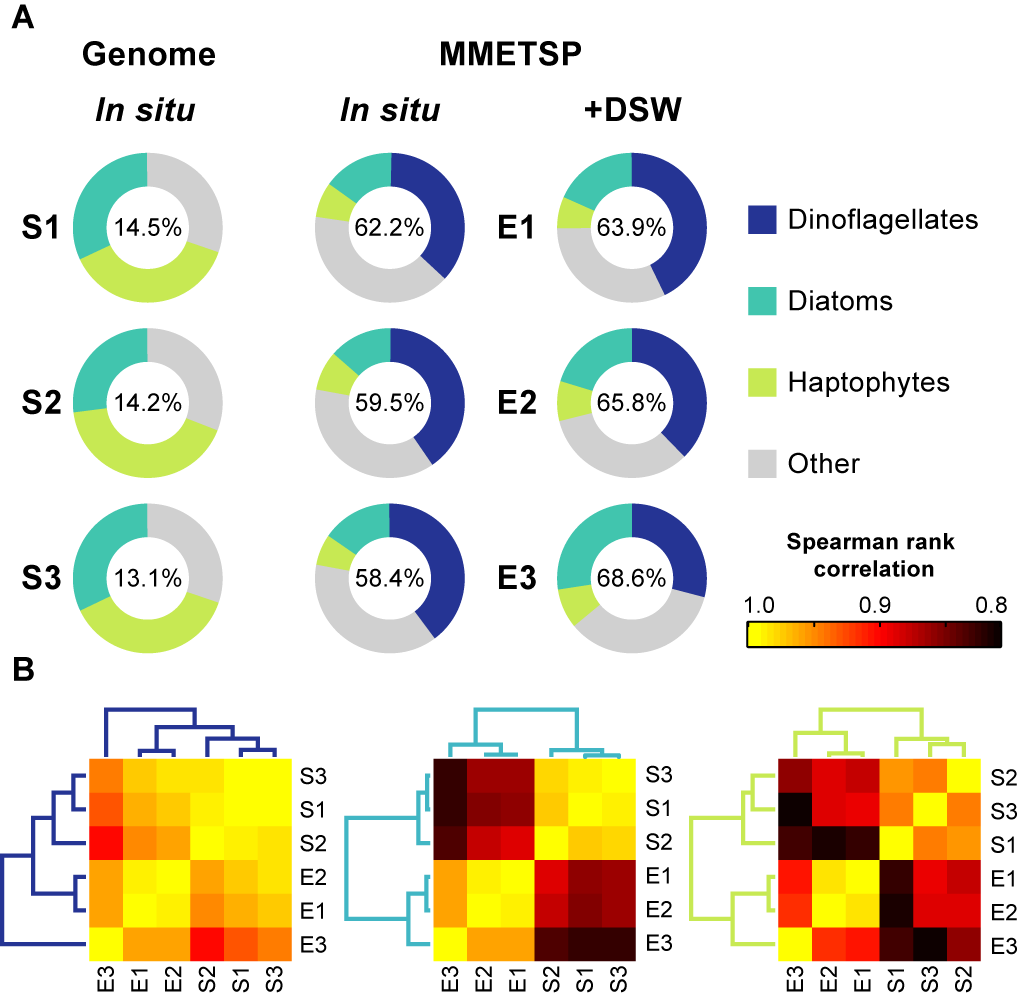
\includegraphics[width=.8\textwidth]{Images/C4_Figure1_Final.png}
    \caption[Taxonomic distribution in mRNA mapped reads consistent across time but altered by deep seawater (DSW) addition]{Taxonomic distribution in mRNA mapped reads consistent across time but altered by deep seawater (DSW) addition. Sequences collected during the summer of 2012 at Station ALOHA (S1: 6 August, S2: 24 August, S3: 2 September) and corresponding deep seawater (DSW) incubation experiments (E1-E3) were mapped to two custom databases: 1) non-symbiotic microalgal genomes and 2) all freely available transcriptomes from the MMETSP as of 17 March 2014. (A) Taxonomic affiliation of reads across the three most abundant functional groups: dinoflagellates, diatoms, and haptophytes mapped to both the genome and MMETSP databases for S1-S3. The corresponding DSW addition incubations E1-E3 were only mapped the MMETSP database. The percent of total reads mapped is indicated inside each of the circles. (B) Spearman rank correlation for species composition shifts within each of the three functional groups across S1-S3 and E1-E3.}
  \label{fig:c4f1}
\end{figure}

The species composition of the functional groups, reflected in rank abundance (\cref{fig:c4f1}B), was highly conserved across all three \textit{in situ} samples (S1-S3), underscoring the stability of phytoplankton populations in this well-studied oligotrophic system. Between 18.1 and 20.7\% of reads mapped to the MMETSP database were annotated with KEGG orthology, elucidating differences in the mRNA distribution between functional groups at the pathway level. Looking at the module-level, the general distribution of transcripts in proportion to the total was assessed using quantitative metabolic fingerprinting (QMF) \citep{Alexander2015}. Diatoms have a larger proportion of mRNA in the transport-related system (e.g. metallic cation, B12, phosphate, and amino acid) compared to haptophytes and dinoflagellates (\cref{fig:c4f2}A). Purine metabolism was consistently a large component of haptophyte QMF (5.6-27\%), an order of magnitude higher than diatoms and dinoflagellates (1-2\%). Purine nucleotides may represent a source of DON accessible to haptophytes, as haptophytes have been found to grow on purines as their sole N source \citep{Palenik1997}. As the precursors for nucleic acid biosynthesis, purine uptake in the ocean has also been attributed to nucleotide salvage \citep{Winn1984}. These functional group differences observed at the module-level are underscored by principle component analysis (PCA) with the QMF for each functional group differing with 95\% confidence (\cref{fig:c4f2}B) and are suggestive of metabolic partitioning between functional groups. Within a functional group, the QMF was stable across time (\cref{fig:c4f2}A), in contrast to the variability observed in coastal systems over similar time scales \citep{Alexander2015, Dupont2015}. This stability likely reflects both the unique physiological attributes of oligotrophic phytoplankton as well as the comparatively static geochemical environment. \par
%Figure 2. QMF and Circos

\begin{figure}[p!]
  \centerline{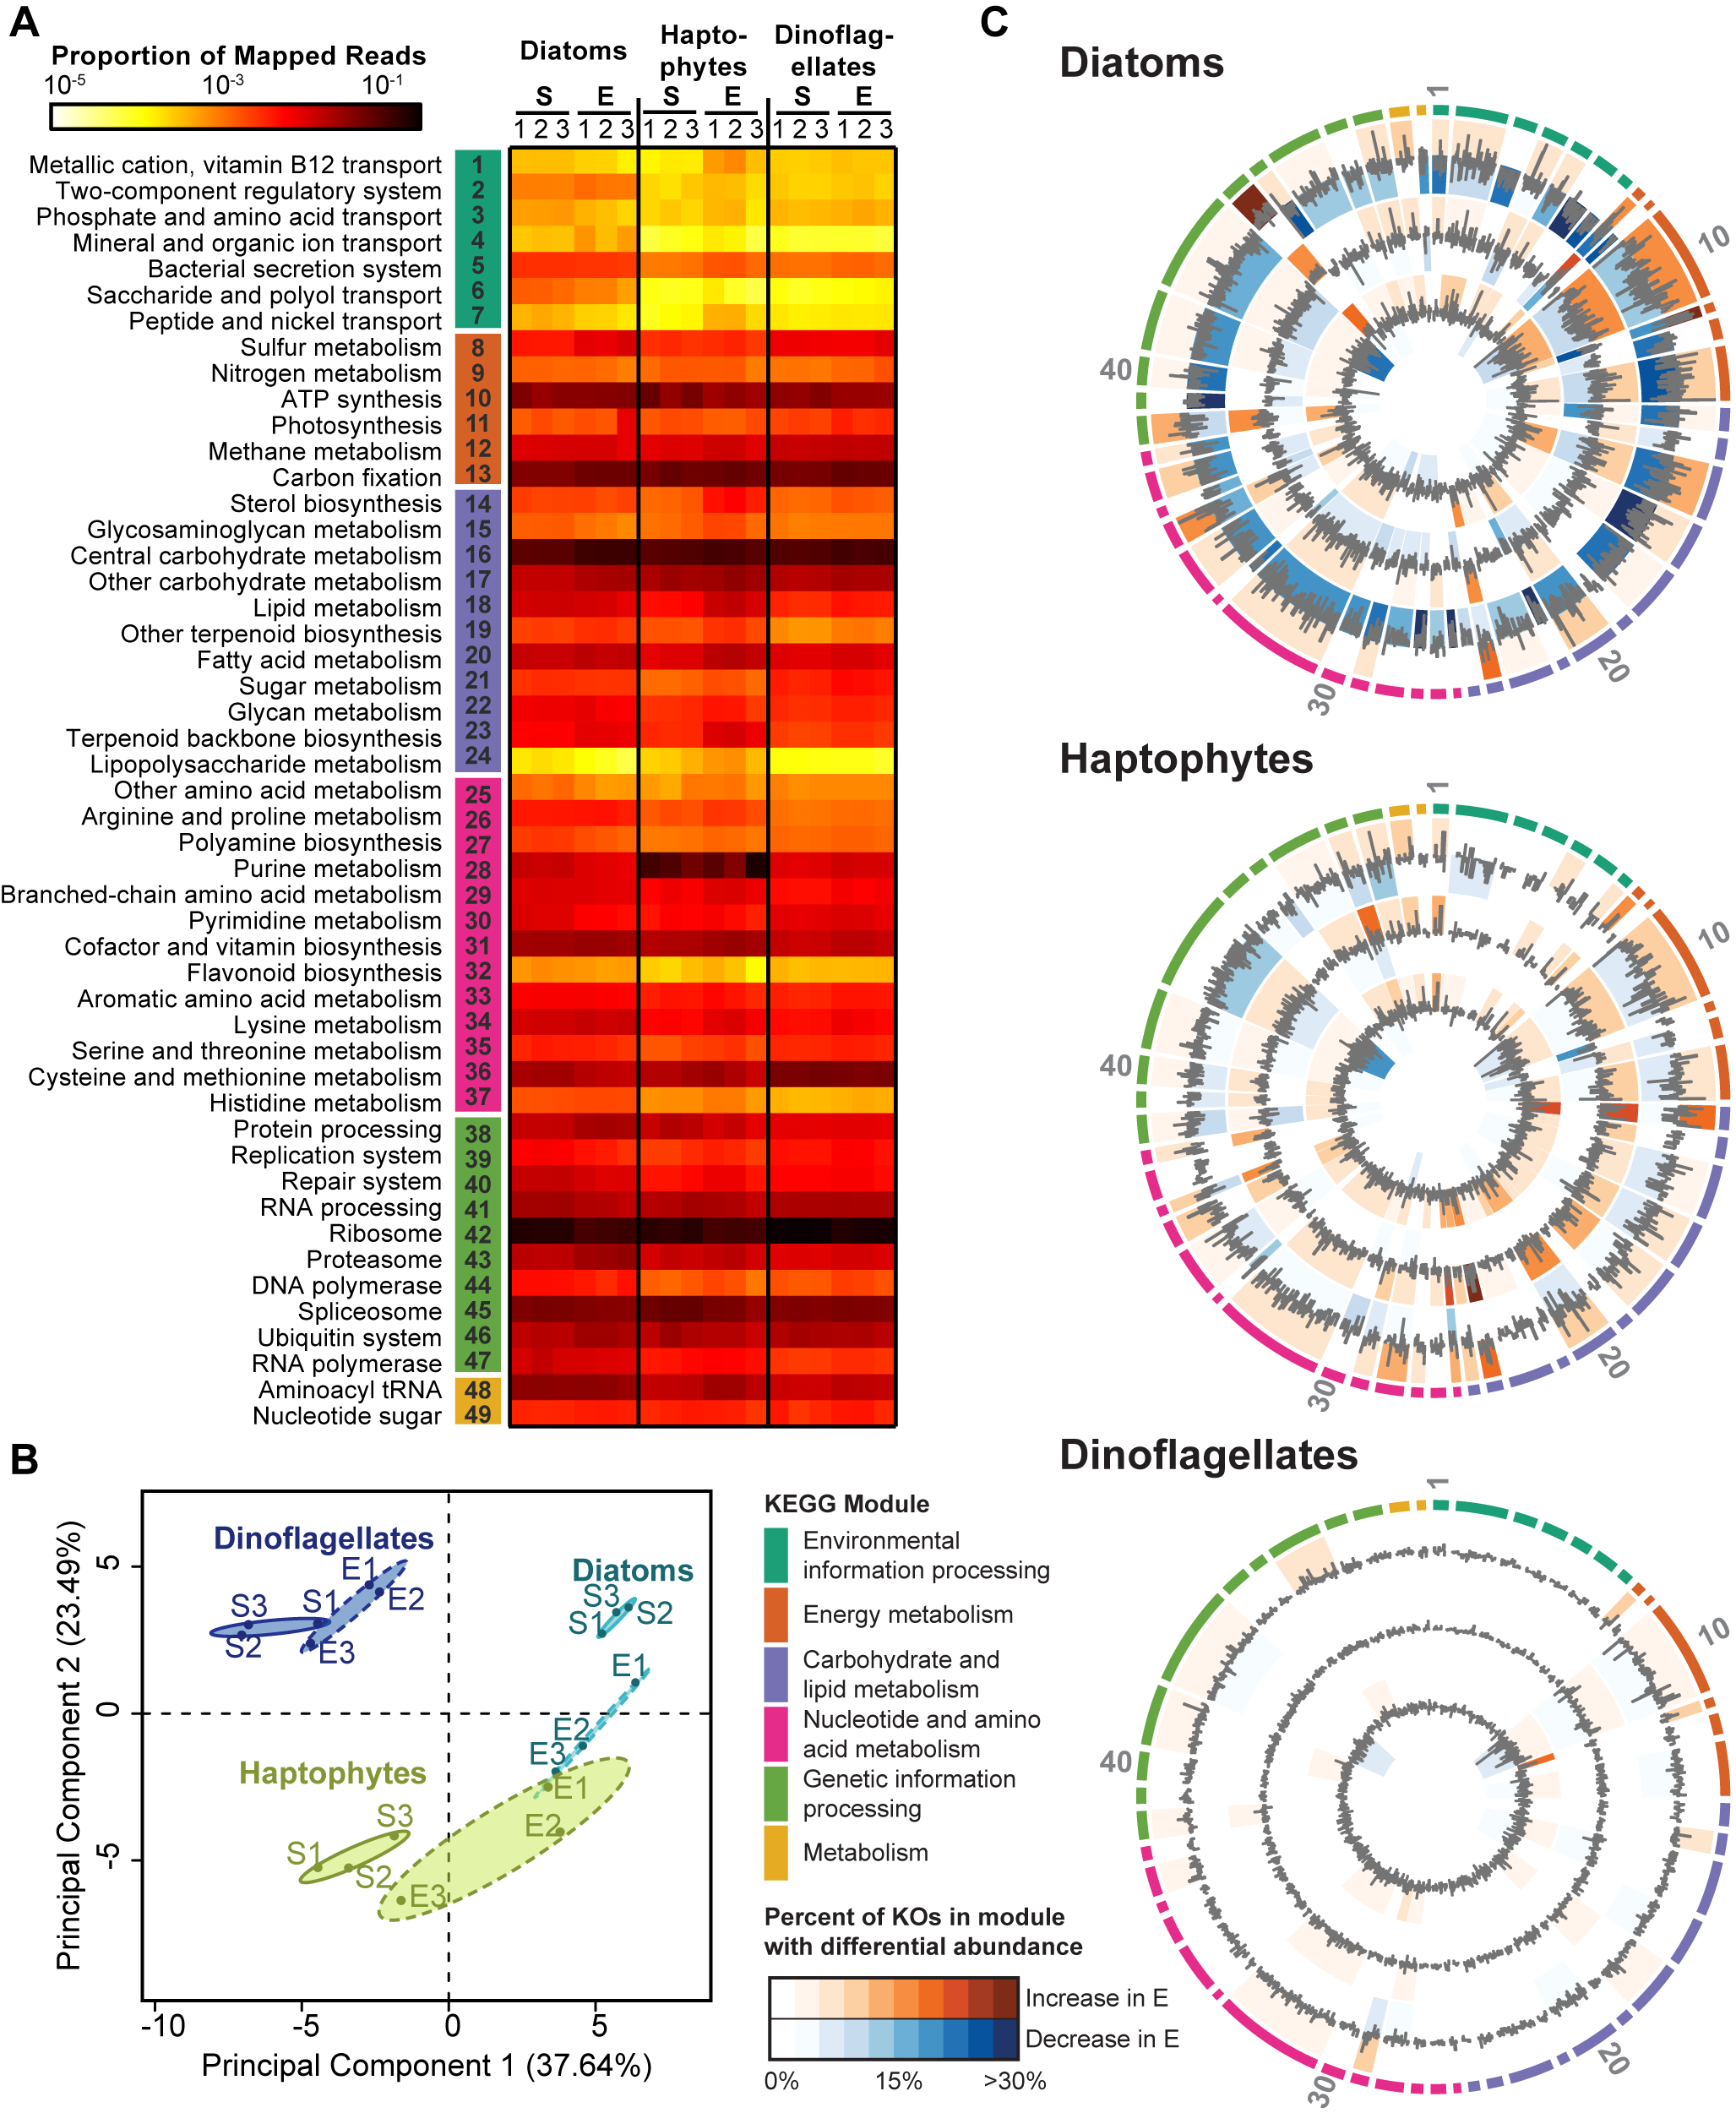
\includegraphics[width=1.1\textwidth]{Images/C4_Figure2_Final.png}}
    \caption[Quantitative metabolic fingerprint (QMF) and patterns of differential expression across KEGG orthology following DSW addition underscore functional group traits]{Quantitative metabolic fingerprint (QMF) and patterns of differential expression across KEGG orthology following DSW addition underscore functional group traits. Caption continued on following page.}
  \label{fig:c4f2}

\end{figure}

\begin{figure}[h!]
    \contcaption{Quantitative metabolic fingerprint (QMF) and patterns of differential expression across KEGG orthology following DSW addition underscore functional group traits. (A) The relative metabolic partitioning of the mRNA pool across the three \textit{in situ} samples (S1-S3) and corresponding deep seawater (DSW) incubation experiments (E1-E3) was assessed using QMF. The summed proportion of mapped reads falling into each of the KEGG modules is depicted as a heat map. (B) Principal component analysis of the QMF signals for each of the functional groups across S1-S3 and E1-E3; 95\% confidence ellipses are indicated for each of the sample types by functional group. (C) Log fold change and significance of differential expression between deep seawater (DSW) amendments and \textit{in situ} samples for KEGG orthologs is visualized with Circos \citep{Krzywinski2009} for the diatoms, haptophytes, and dinoflagellates. Outermost ring colors indicate the KEGG super module, with individual wedges of the pie corresponding to KEGG modules as numbered in A. Concentric circles indicate the expression of the three, replicated DSW addition experiments compared to \textit{in situ} samples: E3 (outer), E2 (middle), E1 (inner). The log fold change of individual KEGG orthologs is depicted as a bar plot bounded -3 to 3. The background color of individual KEGG modules identifies the percentage of genes within module that were significantly (2 fold-change, post-$p > 0.95$) increased (orange) or decreased (blue) in abundance, where darker colors indicate that a higher percentage of genes within that module were significantly different.}
\end{figure}


The static nature of population structure and functional group QMF was altered by replicated nutrient-rich DSW addition experiments, which led to a 7- to 17-fold increase in chlorophyll a, increases not observed in the control treatment (\cref{fig:a4f1}). This increase was consistent with previous studies, which also noted increases in diatoms \citep{McAndrew2007}. Diatom-associated mRNA reads increased in each of the DSW experiments (\cref{fig:c4f1}A). Although species designations can be influenced by the composition of the database used for read mapping, apparent taxonomic shifts occurred at the species-level for diatoms and haptophytes (\cref{fig:a4f2}). Shifts in taxonomic composition were consistent with DSW addition for diatoms and haptophytes, with rank abundance clustering for all experiments (\cref{fig:c4f1}B).  Taxonomic shifts in diatoms were driven by an increase in the rank abundance of certain species, which in all cases were pennate forms (\cref{fig:a4f2}), including genera known to be present in the NPSG like Pseudo-nitzschia \citep{Silver2010} and common in oligotrophic nutrient amendment incubation studies \citep{Marchetti2005, Marchetti2012a}. Although species shifts also occurred within the haptophtyes, \textit{Emiliania huxleyi} was always the most dominant taxon (\cref{fig:a4f2}). The shifts in diatom dominance compared to the consistent dominance of \textit{E. huxleyi} may reflect differences in evolutionary strategies, with metabolic diversity spread across many species in the diatoms and a single species complex with a pangenome, \textit{E. huxleyi}, in the haptophytes \citep{Read2013}. The QMF of DSW addition was significantly different from the QMF of the \textit{in situ} community for both diatoms and haptophytes, but not dinoflagellates (\cref{fig:c4f2}B). Following DSW addition, the QMF for both diatoms and haptophytes was characterized by increased expression of modules associated with growth, such as carbon fixation (\cref{fig:c4f2}A). These shifts are not the result of changes in species composition, as the patterns of expression from individual species tracked the summed community (\cref{fig:a4f3}). The lack of change in the QMF of dinoflagellates (\cref{fig:c4f2}B) likely reflects their range of life strategies \citep{Hackett2004} and minimal transcriptional regulation of gene expression as observed in culture-studies \citep{Moustafa2010}. \par

%Figure 3

\begin{figure}[h!]
  \centering
    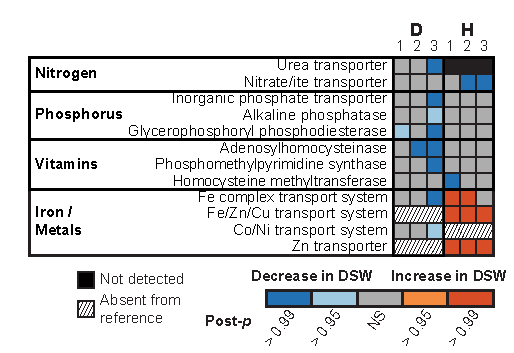
\includegraphics[width=.8\textwidth]{Images/C4_Figure3_Final.pdf}
    \caption[Shifts in transcript abundance of genes responsive to biogeochemical forcing]{Shifts in transcript abundance of genes responsive to biogeochemical forcing. The significance of changes in abundance (2 fold-change, post-$p > 0.95$, or $>0.99$) for genes known to be associated with N, P, vitamin, Fe, or other trace metals metabolism for diatoms (D) or haptophytes (H) is indicated as blue (decrease) or orange (increase). Genes present within the reference transcriptome, but not detected in the field were marked in black, and genes absent from the reference are hashed. KEGG IDs are as follows: Urea transporter (K11959), nitrite/ate transporter (K02575), phosphate transporter (K08176), glycerophosphoryl diester phosphodiesterase (K01126), adenosylhomocysteinase (K01251), phosphomethylpyrimidine synthase (K03147), 5-methyltetrahydrofolate-homocysteine methyltransferase (K00548), iron complex transport system (K02013), iron/zinc/copper transport system (K11706), cobalt/nickel transport system (K02006), zinc transporter (K14715).}
  \label{fig:c4f3}
\end{figure}


Variability within the QMF modules was resolved by statistically assessing the changes in abundance of individual genes for each functional group using a Bayesian approach \citep{Wu2010} (\cref{fig:c4f2,,fig:a4f4}). Statistical significance (2-fold change, posterior probability (post-$p$) > 0.95) of differential abundance was examined for 4038 KEGG orthologs common to diatoms, haptophytes, and dinoflagellates. As with the QMF (\cref{fig:c4f2}A), dinoflagellates demonstrated little to no significant changes in gene expression (\cref{fig:c4f2}C). The suites of transcripts with significantly increased transcript abundance following DSW were highly conserved for both diatoms and haptophytes across the three replicate experiments (40\% of 334 and 19\% of 490 genes common, respectively) but differed between functional groups (41 of the total 824 significantly increased transcripts genes common) (\cref{fig:a4f5}). Of the genes with increased transcript abundance many of those conserved across all three experiments for diatoms and haptophytes were associated with growth (e.g. ATP synthesis (10), photosynthesis (11), and carbon fixation (13)) (\cref{fig:c4f2,,fig:a4f6}). Additionally, following DSW addition, diatoms had signals indicative of the incorporation of both nitrogen (increasing abundance of glutamate and glutamine synthase) and iron (switching from NADPH to ferredoxin sulfate reductase). These changes in transcriptional patterns indicate that both diatoms and haptophytes increase fundamental metabolic processes required for photosynthetic growth in response to DSW. \par
For diatoms and haptophytes, the consistency in genes with increased transcript abundance stands in contrast to the patterns of genes with significantly decreased transcript abundance following DSW addition (\cref{fig:a4f5}). Diatoms were typified by significant decreases in transcript abundance of many genes following DSW, consisting of a large portion (1389 genes) of their metabolism compared to haptophytes (490 genes) (\cref{fig:c4f2}C). Genes with decreased transcript abundance were variable across the three experiments (1.5\% and 6.9\% similar for diatoms and haptophytes, respectively) (\cref{fig:a4f5}) and imply a tailoring of basal metabolism to the change in biogeochemical environment from DSW amendment. Across the KEGG modules, specific genes known to be markers of nutrient limitation significantly decreased in abundance following DSW addition (\cref{fig:c4f3}), potentially signifying a limitation in the \textit{in situ} population that was alleviated following resupply. Such genes or their protein products are frequently used as proxies to identify limitation in the field \citep{Saito2014}. In E1 and E2, there was a decrease in diatom-associated glycerophosphoryl phosphodiesterase \citep{Dyhrman2012} and adenosylhomocysteinase \citep{Bertrand2012a}, indicative of phosphorus (P) and vitamin limitation, respectively (\cref{fig:c4f3}). Silica transporters, though not in KEGG, were surveyed and not found to have significant shifts in abundance. E3 was characterized by a decrease in abundance of many genes indicative of limitation in the diatoms, including but not limited to, a urea transporter \citep{Bender2012}, a phosphate transporter \citep{Dyhrman2012}, and metal transporters (\cref{fig:c4f3}). This is suggestive of diatom co-limitation in E3, similar to patterns of co-limitation recently observed in picocyanobacteria in the Pacific Ocean \citep{Saito2014}. There was a decrease in transcript abundance for haptophyte-associated nitrate and nitrite transporters in E2 and E3 and homocysteine methyltransferase in E1 (\cref{fig:c4f3}). This may be indicative of nitrogen and vitamin limitation based on the pattern in other organisms \citep{Bertrand2012a, Bender2014}, but the regulation of these targets in haptophytes is poorly understood. Metal transport proteins were significantly increased for haptophtyes in E1-E3 and indicated metabolic strategies following the addition of resources that differ from diatoms. In contrast to the diatoms, no markers of P limitation, such as the phosphate transporter or alkaline phosphatase in \textit{E. huxleyi} \citep{Dyhrman2006, Dyhrman2003, Xu2006}, were significantly decreased for haptophytes, consistent with their known tolerance for P limitation \citep{Lessard2005}. These data evince that diatoms and haptophytes are not under the same biogeochemical controls \textit{in situ} and employ disparate strategies following DSW addition to capitalize on newly available resources. Being able to identify and characterize multiple markers of limitation in a genera-specific manner for these eukaryotes is of central importance to the modeling of aperiodic blooms of these groups in oligotrophic systems. \par 



%Figure 4
\begin{figure}[p!]
  \centering
    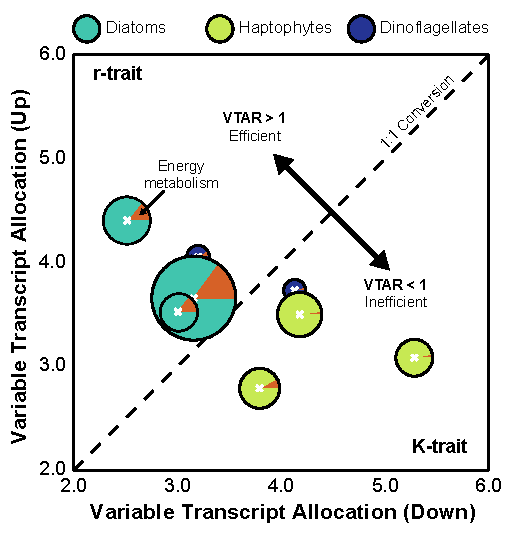
\includegraphics[width=.8\textwidth]{Images/C4_Figure4_Final.pdf}
    \caption[Variable transcript allocation space differentiates functional group strategies]{Variable transcript allocation space differentiates functional group strategies. The variable transcript allocation score (Equations \ref{eq:c4e3} and \ref{eq:c4e4}) of the genes with significantly increased ($VTA_{Up}$) or decreased ($VTA_{Down}$) abundance in the deep seawater (DSW) amendment relative to the \textit{in situ} sample is plotted for diatoms, haptophytes, and dinoflagellates for E1-E3. The size of the pie indicates the total number of genes with significantly different transcript abundances between the \textit{in situ} and DSW amended treatments. The proportion of increased TPM in E within the energy metabolism super group is illustrated as a pie slice in orange.}
  \label{fig:c4f4}
\end{figure}



The above analyses focus primarily on the gene content and transcriptional patterns; however, the underlying eco-evolutionary metabolic traits for a functional group may be better described by considering the shift in the total transcript pool (TPM). Using the statistically resolved patterns of increases and decreases in transcript abundance, a variable transcript allocation ratio ($VTAR$) was calculated to model functional group transcriptional responsiveness to DSW amendment (\cref{fig:c4f4}). $VTAR > 1$ indicates an efficient reallocation of the transcriptional potential from genes with decreased abundance to genes with increased abundance following DSW amendment, while $VTAR < 1$ indicates an inefficient reallocation. The dinoflagellates had variable $VTA$ scores due to their small pool of differentially abundant genes, however the $VTA$ scores consistently resulted in disparate patterns for the diatom and the haptophytes (\cref{fig:c4f4}). In every experiment, the diatoms fell above the 1:1 line, with a $VTAR > 1$ ($1.15 - 1.75$), while haptophytes fell below, with a $VTAR < 1$ ($0.58 - 0.83$) (\cref{fig:c4f4}). The relative efficiency of reallocation, here defined by $VTAR$, reflects differences in the metabolic traits of these functional groups and aligns with preexisting ecological traits as defined by \citep{Margalef1978}. Diatoms are r-selected with high maximum uptake rates that enhance their competition under high or fluctuating nutrients (such as a DSW upwelling event). This trait is reflected in the significant decrease in transcript abundance of many genes across a broad metabolic range coupled with the targeted increase of a subset of genes largely falling within the energy metabolism super module (\cref{fig:c4f4}), a pattern which was also observed with gene-focused analyses using trimmed mean of M value (TMM) normalization \citep{Marchetti2012a, Robinson2010} (\cref{fig:a4f6}). Haptophytes are K-selected, possessing a low half-saturation constant that enhances growth under low nutrient conditions, but are unable to capitalize on nutrient pulses like r-selected competitors. Again, this ecological trait is reflected in changes in the haptophyte transcript pool. Though numerically fewer of their genes significantly decreased in abundance with DSW addition, the total TPM represented by those genes with decreased abundance exceeded that of those induced, defined by $VTAR <1$ (\cref{fig:c4f4}). This is also reinforced by the gene-specific analysis (\cref{fig:a4f6}). It has been speculated that the mechanistic basis for the r- and K- tradeoff dichotomy in the phytoplankton lies in the disparate investment in growth or resource acquisition machinery \citep{Litchman2008}. The large portion of the transcript pool that increased ($VTAR > 1$) for diatoms shows an ability to capitalize on newly available resources, with 14.2-14.9\% of the increased TPM in the KEGG energy metabolism super module (\cref{fig:c4f4}). 
Haptophytes ($VTAR < 1$), by contrast, do not efficiently reallocate the transcript pool, with only 5.5-10.2\% of the increased TPM in energy metabolism (Figure  \ref{fig:c4f4}). In short, haptophytes do not appear to modulate their transcript pool to capitalize on growth processes as efficiently as diatoms (Figure  \ref{fig:c4f4}). \par



These functional group-specific molecular and metabolic mechanisms underpin the aperiodic eukaryotic phytoplankton blooms in the oligotrophic ocean. Whereas both diatoms and haptophytes, including calcifying groups, likely contribute to a shift towards a net autotrophic condition when there is a nutrient pulse, the ecosystem function of oligotrophic systems may ultimately hinge on the unique trait of the diatoms to more efficiently turn over their scavenger metabolism to one of enhanced production. This finding is consistent with the dominance of diatom-associated BSi export relative to PIC export during summer in the NPSG \citep{Karl2012}. Unlike the preceding 13 years of study at Station ALOHA \citep{Karl2012}, enhanced production and export characteristic of bloom events were not observed during the summer of 2012, which exhibited a period of sustained net-heterotrophy. We demonstrated through simulated blooms that the metabolic capacity for enhanced production is inherent in the large eukaryotic phytoplankton regardless of water mass, suggesting that the lack of bloom in 2012 was variably due to deficiency in macronutrients, vitamins, and metals. As the conditions observed during summer 2012 may be increasingly encountered in a future ocean \citep{Doney2012}, modeling the molecular traits and tradeoffs of these populations will help better predict ecosystem state and metabolic balance of the ocean. \par











\chapter{Warm core rings release predators from thermal constraints when foraging in the ocean Twilight zone}
\label{chap:5}
\raggedbottom

{\let\thefootnote\relax\footnotetext{This chapter was modified to short format and accepted for publication as Braun, C.D., Gaube P., Sinclair-Taylor T., Skomal, G.B., and Thorrold S.R. Warm core rings release predators from thermal constraints when foraging in the ocean Twilight zone. \emph{Journal name}. }}
%\end{singlespace}
{\let\thefootnote\relax\footnotetext{C.D.B. and S.R.T. designed the study. C.D.B, T.S.T. and G.B.S. conducted the tagging; C.D.B. performed the analysis with contributions from P.G. and S.R.T. C.D.B. wrote the paper with contributions and final approval from all authors.}}


\clearpage

\section{Abstract} 

Mesoscale ocean dynamics, such as eddies, are energetic, ubiquitous features that structure open ocean ecosystems. The Gulf Stream is a region of pronounced mesoscale activity that has been shown to produce biological "hot spots" as a result of the coupling of ocean biology and physics, primarily at lower trophic levels. Yet, the fish communities associated with these dynamic features and the physical-biological mechanisms structuring these pelagic ecosystems remains poorly understood. Here, we use satellite telemetry, combined with multi-satellite remote sensing and high-resolution oceanographic modeling, to collocate movements of a model predator, the blue shark (\textit{Prionace glauca}), to mesoscale features in the Gulf Stream. We combine 8,279 satellite-based positions collected from 17 blue sharks over 2,117 tracking days with nearly 500,000 concurrent high-resolution (2.5 minute) depth-temperature measurements to reconstruct blue shark movements in three-dimensions. Our results indicate mesoscale eddies are a primary driver of blue shark movements, and sharks exhibited extensive use of anticyclonic eddies (warm core rings) where enhanced foraging opportunities likely co-occur with anomalously warm water at depth. \textbf{another eddy result here}. Overall, we identify important physical-biological interactions relevant to pelagic predators. Our results highlight the dynamic nature of both ocean physics at and below the mesoscale and the response of higher trophic level organisms to these features. Identifying the most relevant dynamics for marine fishes provides the opportunity for dynamic ocean management approaches that can be adapted to incorporate the appropriate spatial and temporal scales of physical-biological interactions in the ocean.

\clearpage

\section{Introduction}

Meso- and submesoscale dynamics comprise the "internal weather" of the ocean \citep{McGillicuddy2001} and act to structure open ocean ecosystems. Mesoscale dynamics are most notably manifested as eddies and meanders on time scales of weeks to months and spatial scales $O$(10s - 100s km). At the oceanic submesoscale, fronts and filaments dominate variability with scales spatial scales of $O$(1 - 10 km) that persist for days to weeks. In combination, physical processes across these scales provide controls on biogeochemical fluxes \citep{McGillicuddy2016, Mahadevan2016} and affect biological communities, including lower trophic levels \citep{Abraham1998, Martin2003, Labat2009}, marine mammals \citep{Cotte2007, Polovina2006, Bailleul2010, Cotte2015}, birds \citep{Scales2014, TewKai2009}, turtles \citep{Gaube2017, Kobayashi2011, Scales2015}, and fishes \citep{Worm2005, Miller2015, Queiroz2016}. Coupling of biology and ocean physics at the (sub)mesoscale has, in some cases, identified specific features as "hot spots" of biological activity, spanning trophic levels from primary producers \citep{benitez2007mesoscale, Falkowski1991, McGillicuddy2007, Thompson2007} to zooplankton and small fish \citep{godo2012mesoscale}, up to large pelagic fish \citep{Hobday2014, Gaube2018, BraunSwords}. Much of the existing work has been bolstered by recent advances in satellite oceanography that have facilitated the automatic identification and tracking of mesoscale eddies \citep{Chelton2011} and fronts \citep{Belkin2009} globally. These advances in our ability to observe and track (sub)mesoscale features have revealed rich regional variability in how eddies influence near-surface chlorophyll (CHL) distributions \citep{Gaube2014, McGillicuddy2016} and how these features might influence biological communities \citep{Kobayashi2011, Gaube2017, Belkin2014, Queiroz2016, Gaube2018}.

The Gulf Stream (GS) contains some of the most highly energetic eddies on earth \citep{Chelton2011} which can have significant impacts on ecosystem dynamics \citep{Davis1985, Boyd1986, Gaube2018, Gaube2014, Gaube2017DSR}. Cyclonic eddies (or cold-core rings) in this region typically trap Slope water from north of the GS during formation and are thus characterized by negative temperature and positive nutrient and chlorophyll anomalies relative to ambient water south of the GS \citep{Gaube2017DSR, Pingree1979, RingGroup1981}. In contrast, anticyclones (or warm-core rings) are characterized by anomalously warm water that is low in chlorophyll and nutrients due to its source water in the northern Sargasso Sea \citep{Gaube2017DSR, Olson1986}. Both may also contain biological communities trapped during eddy formation \citep{Davis1985, WiebeFlierl1983} or attracted to these unique environments \citep{Hsu2015, Gaube2018}.

Historically, anecdotal evidence and analyses of fisheries-based catch data have supported the association of large pelagic fishes with mesoscale structures like fronts and eddies \citep{Hobday2014}. Yet, the biology of these important oceanographic features and their associated fish communities remain poorly understood, particularly using fisheries-independent means. Electronic tag technologies have driven significant advances in understanding movements and ecology of pelagic fishes \citep{Skomal2009, Block2011, Thorrold2014, Berumen2014, Werry2014}; however, the inherent error associated with traditional light-level geolocation \citep[$\pm$ 100 km,][]{Braun2015, Braun2018b} often precludes associating animal movements with (sub)mesoscale oceanographic structures \citep[except see][]{BraunSwords}. For those fish species that regularly occupy the surface-air interface, accurate satellite-based positions (\eg Argos, GPS) can be derived, instead of error-prone light-level geolocations. These satellite-based positions permit quantitative, fisheries-independent analyses of the use of (sub)mesoscale features by pelagic predators. The few existing studies that have leveraged these data to investigate (sub)mesoscale feature use by fishes have made important findings regarding, for example, use of seasonally persistent fronts by basking sharks \citep{Miller2015} and preference for anticyclonic eddies in the Gulf Stream by white sharks \citep{Gaube2018}. Furthermore, studies investigating oceanographic influences on predators often neglect the integration that occurs across several scales simultaneously to drive the behaviors we observe using telemetry. Yet, incorporating variability across the (sub)mesoscale is fundamental to developing a holistic understanding of physical-biological interactions governing animal movements \citep{Fauchald2000}.

While blue shark movements have been studied extensively following the pioneering work of \citeauthor{Carey1990} \citep{Queiroz2010, Campana2016, Vandeperre2014a}, relatively little information exists on the oceanographic drivers of their observed behaviors. Here, we use satellite telemetry to study the blue shark (\textit{Prionace glauca}) as a model pelagic predator in a multi-satellite analysis framework. We collocate shark movements with remote-sensing data to investigate the meso- and submesoscale physical-biological mechanisms driving movements and habitat use of this pelagic predator. 

\section{Materials and methods}

\subsection{Satellite tagging and data} \label{sec:satdata}

Adult male blue sharks (mean 264 cm fork length, range 220-313 cm) were tagged near Montauk, New York during Summer 2013 and 2014 (n=2) and Cape Cod, MA during Fall 2015 and 2016 (n=17; Table \cref{tab:c5t1}). All were tagged with fin-mounted Smart Position or Temperature Transmitting (SPOT, Wildlife Computers) tags, and we deployed pop-up satellite archival transmitting (PSAT, model miniPAT, Wildlife Computers) tags, in addition to SPOT tags, on the individuals near Cape Cod (n=17; Table \cref{tab:c5t1}). Sharks were captured on rod and reel and brought onboard the fishing vessel where they were ventilated with a seawater hose and the hook was removed. SPOT tags were affixed to the dorsal fin using nylon bolts and contained a wet/dry switch that activated at the surface to transmit to the Argos satellite network from which a Doppler-based position was calculated. PSATs were tethered with a stainless steel wire to an intramuscular T-bar style spear tip (n=16) or a nylon umbrella dart (n=3). \textit{In situ} measurements of pressure, temperature and light levels were collected every 15 seconds throughout the PSAT deployments and aggregated for satellite transmission. Archived depth and temperature data were transmitted as 4 summarized products: (1) time-at-temperature and (2) time-at-depth histograms for 12 bins every 24 hours; (3) depth-temperature profiles at 16 representative depths every 24 hours; (4) depth time series at 2.5 minute resolution. PSATs were programmed to detach after 180 days and transmit these summarized data products, along with daily light level data for geolocation, via the Argos satellite system.

Resulting SPOT-tag locations were processed with a Kalman filtering algorithm by Collecte Localisation Satellites \citep{Lopez2014} and subsequently assigned error flags called location classes (LC): LC 3, <250 m; LC 2, 250-500 m; LC 1, 500-1500 m; LC 0, >1500 m for classes 3, 2, 1, 0. Additional classes A, B represent positions derived from less than 4 satellite messages which result in no estimates of spatial accuracy from CLS; however, recent work on several marine species and platforms by \citet{Lopez2014} suggests error for A, B classes is order 1-10 km and nearly always < 20 km. Location class Z positions were considered invalid and removed from further analysis \citep{CLS2016}. Remaining positions were filtered using a speed filter (4 $m s^{-1}$) from the \texttt{trip} package \citep{Sumner2015} to remove unrealistic locations. The filtered Argos data were fit in a hierarchical fashion with a two-state switching state-space model (SSM) to estimate locations from the noisy Argos data, infer behavioral state and standardize the location time series (6 hr resolution) \citep{Jonsen2016}. The SSM combines a process model that estimates movement parameters and an observation model that accounts for spatial uncertainty using Markov Chain Monte Carlo (MCMC). The model inferred a behavior state based on fitted movement parameters (correlation, $\gamma$ and turn angle, $\theta$). Resident behavior (often referred to as area-restricted search or foraging) was characterized by $\theta$ near 180$^{\circ}$ and $\gamma$ near 0 (short steps with large turn angles), while traveling (or transit) behavior produces movements in which $\theta$ is near 0$^{\circ}$ and $\gamma$ near 1 (long, relatively straight tracks) between consecutive steps in the individual trajectories. Blue shark tracks were divided into trajectories for which data gaps were no longer than 4 days. Models were fit in JAGS \citep{Plummer2004} using the \texttt{bsam} package \citep{Jonsen2016} for \texttt{R} \citep{RDevelopmentCoreTeam2015}. The models were fit with a 6 hour time step using two MCMC chains of 60,000 samples from which the first 40,000 were discarded as burn-in. Posterior inference was performed from the remaining 20,000 samples per chain after thinning by a factor of 20 to reduce within-chain sample autocorrelations, yielding a final 2,000 samples from the joint posterior. Model convergence was assessed using criteria outlined in \citet{Jonsen2016} and included$\colon$ posterior samples were stationary, MCMC chains were well-mixed, within-chain autocorrelation was low and the Brooks-Gelman-Rubin potential scale reduction factors ($\hat{r}$) were $\leq$ 1.1.

\subsection{Oceanographic data}

To quantify associations between blue sharks and mesoscale eddies, we used the Mesoscale Eddy Trajectory Atlas distributed by Archiving Validation and Interpretation of Satellite and Oceanographic Data (AVISO; \href{https://www.aviso.altimetry.fr/en/data/products/value-added-products/global-mesoscale-eddy-trajectory-product.html}{https://www.aviso.altimetry.fr/en/data/products/value-added-products/global-mesoscale-eddy-trajectory-product.html)} that describes daily tracks of coherent mesoscale structures (CMS) based on maps of surface altimetry \citep{Chelton2011}. Eddies with lifetimes greater than 4 weeks (28 days) are tracked based on their signatures in sea-level anomaly (SLA) fields. Prior to the identification and tracking of mesoscale eddies, the SLA fields are high-pass filtered using a 20$^\circ$ x 10$^\circ$ (longitude x latitude) 2D weighted least-squares regression (LOESS) smoother to remove the effects of seasonal heating and cooling \citep{Chelton2011} as:

\begin{equation}
SSH = SLA - \left<SLA\right>
\label{eq:ssh}
\end{equation}

where the $<>$ operator indicates spatial smoothing. We developed a meander filter for the Gulf Stream region (see Section \cref{sec:eddycoll}) using daily, 0.25$^\circ$ resolution absolute dynamic topography (ADT) data from AVISO which is generated by satellite-derived anomalies from the \citet{Rio2011} mean dynamic topography surface. Daily, 1 km sea surface temperature (SST) data was acquired from NASA JPL's Multi-scale Ultra-high Resolution (MUR) product. SRTM30+ bathymetry from Scripps was downloaded from NOAA CoastWatch server (ERDDAP id: srtm30plus) \citep{Becker2009}.

\subsection{Eddy collocation} \label{sec:eddycoll}

Eddy occupation was quantified using a subset of the track data to include those positions that were in the Gulf Stream, a well-known region of mesoscale activity, in water deeper than 2000 m and that corresponded to the temporal limits of the eddy tracking dataset (Jan 1993 - Jan 2017). To focus our analysis on eddies, we developed a two-step meander filter \citep[similar to ][]{Gaube2017DSR} for the Gulf Stream region in which we: 

\begin{enumerate} 
\item defined a mask 1$^\circ$ north and 2$^\circ$ south of the GS north wall (40 cm ADT contour). Those features in which the core of the CMS was within the meander mask were considered meanders and removed from the remainder of the analysis. 
\item calculated net zonal displacement of eddies and removed those that exhibited primarily eastward displacement, following \citet{Gaube2017DSR}, using a 3-day rolling window. 
\end{enumerate}

Shark locations were collocated to the nearest eddy identified in the eddy atlas (excluding meanders as described above) following \citet{Gaube2017}. We also used a maximum distance from the eddy center of 200 km or 2.5 times the length of the eddy radius to prevent collocation to eddies from an unreasonable distance to be biologically-relevant.

To assess differences in the distribution of blue sharks within anticyclonic and cyclonic eddies, we constructed histograms of blue shark location as a function of radial distance from the eddy center, resulting in number of shark positions per unit area of an annulus defined by the radial distance from the eddy center. To determine if individuals are more likely to be associated with the core, interior or periphery of eddies of either polarity, we defined eddy subregions by the normalized distance $r$ from the eddy SLA extremum, where the inner-core is defined as $r \leq L_s/2$, the outer core as $L_s/2 < r \leq L_s$ and the eddy interior includes both the inner and outer core $r \leq L_s$. The eddy periphery is defined as $L_s < r \leq 2L_s$ and the area outside of an eddy as $r > 2L_s$ \citep[see Fig. 2 in][]{Gaube2017}.

We compared observed movements to two null models of eddy use by collocating simulated tracks and drifter data to the eddy field as described above. We generated 100 correlated random walk (CRW) simulations per blue shark using the distributions of turn angles and step lengths from each individual's observed movement data (\texttt{adehabitatLT} \texttt{R} package; \citet{Calenge2006}). To match the spatial bias in presence data, CRW simulations were initiated at the tagging location for each individual and were constrained to realistic movements using bathymetry. CRW simulated tracks for each individual represent random eddy use based on chance of encountering these features. To assess the role of passive advection and the relative spatial composition of the sub-regions of eddies of each polarity, we collocated a surface drifter dataset from NOAA's Atlantic Oceanographic and Meteorological Laboratory (\url{ftp://ftp.aoml.noaa.gov/pub/phod/buoydata/hourly_product/}), using all drifters within the study region for a 5-year period (2005-2009). Significance testing of eddy use by tracked sharks was conducted by comparing the observed frequency of eddy use per individual to the confidence interval of eddy use by CRW simulations.

\subsection{Diving and vertical eddy structure}

PSAT tags were not programmed to transmit \textit{in situ} temperature time series data. Thus, temperatures to accompany the depth time series were interpolated from daily depth-temperature profiles by computing a weighted least-squares regression of data using half-power filter cutoffs of 5 days and 150 m. The resulting depth-temperature time series of blue shark diving (from PSAT tags) was collocated to eddies at 6-hour intervals to match the temporal resolution of the standardized position data (from the SPOT tags). Individual dives in eddies were extracted from the time series data using the \texttt{diveMove} package \citep{Luque2007} in \texttt{R}. Dives were characterized by movements below 200 m from shallower than 50 m for longer than 30 minutes and less than 6 hours.

Eddy vertical composites were computed from the HYbrid Coordinate Ocean Model (HYCOM)\citep{Chassignet2007} using modeled depth-temperature profiles for the eddies occupied by the sharks during the periods of occupation. Profiles were interpolated to 5 m intervals and summarized by calculating the mean profile at intervals of $L_s/10$ from $-2 L_s$ to $2 L_s$. Temperature anomaly for the shark time series and eddy vertical composites were calculated by subtracting the climatological mean temperature from the World Ocean Atlas 2013 \citep{Locarnini2013} at each depth level.

\section{Results}

\subsection{Overall movements}

Blue sharks moved across a 25$^{\circ}$ and 40$^{\circ}$ latitudinal and longitudinal range, respectively, between highly dynamic Gulf Stream waters to oligotrophic, relatively homogeneous habitat in the Sargasso Sea. All 17 SPOT tags reported an average of 4 positions $\cdot$ day $^{-1}$ over 54-288 days at liberty (Table \cref{tab:c5t1}). Overall movements covered, on average, 5,454 km (2,280-14,485 km) in up to 288 days at liberty and were predominantly oriented east-west at temperate latitudes (Fig. \cref{fig:c5f1}). Depth and temperature data indicated blue sharks made extensive vertical movements offshore. Twelve PSAT tags deployed in this study reported and transmitted data, 7 of which reported >10 days early. The 12 reporting tags were at liberty for an average 129 days (range 16-180). PSAT-tagged sharks regularly dove to at least 400 m when offshore of the continental shelf (maximum depth 1,696 m), almost exclusively during daylight hours. Overall mean temperature occupied was 18.5$^\circ$C (range 3.9-31.8$^\circ$C), and blue sharks largely remained above the 10-12$^\circ$C isotherm while diving.

\subsection{Movements in the Gulf Stream eddy field}

Overall, 38\% of positions within the GS region were within cyclonic and anticyclonic eddies (19\% within eddies of each polarity; Fig. \cref{fig:c5f1}, Table \cref{tab:c5t2}). This represents similar use of eddies, based on frequency, to that indicated by CRW simulations (mean 20\% in CEs and 18\% in ACEs). However, individual variability in eddy use was high, and some individuals demonstrated highly significant use or avoidance of eddies. Percent frequency of positions collocated to eddies ranged from 2-39\% in ACEs and 4-28\% in CEs.

Blue shark locations in eddy-centric coordinates suggest qualitatively similar use of both eddy types (Fig. \cref{fig:c5f1}A, B); however, histograms of shark positions as a function of distance from eddy centers (normalized by the area of the annulus defined by each radial bin) revealed that blue sharks were significantly more likely to be associated with the inner-cores ($r \leq L_s / 2$) of ACEs than CEs, potentially driven by an avoidance of CE cores (Fig. \cref{fig:c5f1}C, E). Sharks were also significantly more likely to exhibit residency, rather than transiting, behavior while in ACE cores (Fig. \cref{fig:c5f1}C, E). In eddy peripheries, we observed no differences in overall use of eddies of either polarity. However, comparing collocated CRW simulations and drifter data suggests less use of ACE and CE peripheries ($r > L_s$) by sharks than by either null model (Fig. \cref{fig:c5f1}D, F). This is further corroborated by the behavior state data which indicates blue sharks were more likely to exhibit transit behavior near $L_s$ in eddies of either polarity. In fact, both drifters and CRW results suggested higher null "use" of CEs than ACEs which further supports active use of ACEs by blue sharks as they demonstrated equal or higher use of ACEs relative to CEs (Fig. \cref{fig:c5f1}).

\subsection{Vertical structure of eddies and diving behavior}

HYCOM-derived composites for the shark-occupied eddies indicated eddy vertical structure typical of energetic Gulf Stream eddies. ACEs were characterized by warm surface water (22-23$^\circ$C) and depressed isotherms (Fig. \cref{fig:c5f2}A) resulting in positive (warm) temperature anomalies as high as 3$^\circ$C from 250-600 m (Fig. \cref{fig:c5f2}C). In contrast, CEs exhibited 19-20$^\circ$C SSTs with "domed" isotherms (Fig. \cref{fig:c5f2}B) and negative (cold) temperature anomalies >2$^\circ$C between 300-700 m (Fig. \cref{fig:c5f2}D).

Depth-temperature time series data derived from shark PSAT tags was collocated to eddies for a total of 15,189 depth measurements within eddy cores ($r \leq L_s$) at 2.5 minute resolution. When compared to eddy vertical composites, shark depth-temperature data from eddy cores were representative of these features in the Gulf Stream. Tagged individuals experienced a wide temperature range ($\pm$ 6$^\circ$C from mean ACE composite) while diving around the cores of ACEs (Fig. \cref{fig:c5f2}A) and a restricted range ($\pm$ 2$^\circ$C from mean CE composite) in CE cores (Fig. \cref{fig:c5f2}C). Blue sharks encountered positive temperature anomalies throughout their excursions below 150 m in ACEs, including warm anomalies as high as 10$^\circ$C from 250-350 m (Fig. \cref{fig:c5f2}C). In CEs, blue sharks occupied slightly warmer water than that predicted by HYCOM-derived composites (Fig. \cref{fig:c5f2}B). These features proved anomalously cold (-5$^\circ$C anomaly) in near-surface waters (Fig. \cref{fig:c5f2}C) but were otherwise within $\pm$ 2$^\circ$C of climatological mean temperatures at depth (Fig. \cref{fig:c5f2}D). 

Regardless of eddy polarity, tagged individuals spent 40-50\% of time in eddies in the upper 50 m of the water column and < 10\% of time while in eddies below 300 m. In general, tagged sharks spent more time-at-depth between 50-350 m in ACEs compared to CEs (Fig. \cref{fig:c5f2}); however, a small but notable increase in time-at-depth was observed deeper than 550 m in some Gulf Stream cyclones (Fig. \cref{fig:c5f2}). The limited deep diving (> 400 m) observed in ACEs occurred in typical warm core rings characterized by positive temperature anomalies at depth and temperatures > 12$^\circ$C at 600 m (Fig. \cref{fig:c5f3}A). Diving in CEs was often shallower due to shoaling of isotherms (Fig. \cref{fig:c5f2}) resulting in compression of the available water column warmer than 10$^\circ$C (Fig. \cref{fig:c5f3}B). Deep dives in CEs were constrained to those eddies that were low amplitude and/or old which made their vertical structure nearly indistinguishable from warm ambient water south of the GS (Fig. \cref{fig:c5f3}C).

In addition to aggregate depth-temperature data, we extracted individual dives below 200 m in eddies. While the time series record contained 2.5x more dives below 200 m in ACEs compared to CEs, there was no significant difference in the depth or duration of dives between the two eddy types (Fig. \cref{fig:dives}).

\section{Discussion}

Meso- and submesoscale dynamics structure ocean ecosystems and generate patchiness that is fundamental to ocean ecology \citep{McGillicuddy2016, Mahadevan2016}. Yet, how these physical-biological interactions influence pelagic fish communities remains poorly understood. Our results identify mesoscale eddies as key drivers of movements and behavior of a model pelagic predator, the blue shark.

Blue sharks in our study exhibited wide-ranging and highly variable movements despite study individuals being primarily from the same demographic and tagging location. These data broadly fit with results from other tagging efforts in the Atlantic which report widespread pelagic movements of blue sharks outside of coastal aggregation periods \citep{Vandeperre2014, Campana2011, Howey2017}. Previous work has suggested the importance of the Gulf Stream as overwintering habitat for immature individuals \citep{Campana2011} and as a conveyor for females (most of which have recently mated) moving offshore and some toward the eastern Atlantic \citep[reviewed in][]{Nakano2008}. All individuals in our study were mature males that occupied the Gulf Stream region during winter months, further corroborating its role as overwintering habitat for this species.

\subsection{Mesoscale dynamics of the Gulf Stream and the role of eddies}

% role of ACEs relative to CEs
The Gulf Stream is one of the most dynamic regions of the world ocean and contains some of the most highly energetic eddies on earth \citep{Chelton2011}. These features can have significant impacts on pelagic communities \citep{Gaube2017DSR} and ecosystem dynamics \citep{Davis1985, Boyd1986, Gaube2018}. Our eddy collocation analysis demonstrated the role of eddies in driving blue shark movements and behavior in the Gulf Stream. Overall, our results suggest preferential occupation of the cores of ACEs. Similar results have been shown for white sharks in the Gulf Stream \citep{Gaube2018}, southern bluefin tuna in Australia \citep{Hobday2014} and turtles in the Bay of Biscay \citep{Doyle2008}, Brazil-Malvinas confluence \citep{Gaube2017} and off the southeastern coast of Africa \citep{Luschi2003}. All of these studies suggest higher use of ACEs is likely due, at least in part, to elevated foraging opportunities. However, others have proposed thermoregulatory \citep{Campana2011, Gaube2018, Gaube2017} and navigational functions \citep{Carey1990}.

%\subsection{Potential mechanisms driving eddy use}
% why ACEs: 3 explanations, foraging thermoregulation navigation

%% thermo
Our results suggest two, likely interacting, explanations for the observed eddy use based on foraging and thermoregulation. Sharks in our study regularly conducted diel vertical migration while offshore from the surface during night to periods of regular dives into the mesopelagic (200-400 m) during daytime. These results are consistent with previous studies tracking blue sharks in the Gulf Stream that also reported a high frequency of octopods, a diel vertical migrator that occurs principally below 250 m, in blue shark stomachs \citep{Carey1990}. Thus, these deep dives may be associated with foraging for cephalopods, one of the blue sharks primary prey items \citep{Clarke1974, Henderson2001}, that are known to concentrate at depth particularly along the Gulf Stream front \citep{Vovk1978, Fedulov1986, Dawe1985}. 

While these data suggest Gulf Stream-wide foraging in the mesopelagic, our collocation analysis indicated a significantly higher number of positions were recorded in the cores of ACEs than CEs in the Gulf Stream, a trend that was further pronounced when considering shark positions separately based on transiting or resident behavior state. We observed sharks more often exhibited residency in ACE cores which may be indicative of foraging \citep{Breed2009} in these features. While ACEs are typically characterized by low productivity and CEs more often contain enhanced chlorophyll and phytoplankton biomass \citep{Gaube2017DSR}, some ACEs have been observed containing enhanced productivity in their cores during winter \citep{Dufois2016}. In fact, \cite{Fennell2015} found enhanced mesopelagic backscatter in North Atlantic ACEs near the Grand Banks where they measured DSL densities that were comparable to the highest average (integrated from 200-1000 m) densities in the world oceans. \cite{Fennell2015} also found a positive correlation between backscatter and temperature at 400-600 m and observed observed extensive backscatter below 100-200 m in these features. Blue sharks in our study regularly dove > 200 m (and as deep as 700 m) in ACEs where these individuals experienced the strongest positive temperature anomaly measured in this region.

Previous studies have suggested the thermoregulatory implications of mesopelagic diving. \citep{Carey1990} fitted a blue shark with a cranial thermistor which indicated thermal hysteresis allowed this individual to maintain body temperatures that were significantly above (average +4$^\circ$C) ambient water temperatures as cold at 8$^\circ$C at 300 m. When muscle cooled to ~15$^\circ$C, the shark aborted the dive and returned to the surface to regain heat loss until muscle temperatures recovered to near 20$^\circ$C before repeating the dive-surfacing cycle. We observed similar oscillatory diving into the mesopelagic during daytime in both types of Gulf Stream eddies that was seemingly constrained by temperature at depth (Fig. \cref{fig:c5f3}), consistent with the behavioral thermoregulation observed by \cite{Carey1990}. Sharks spent more time shallower than 50 m in CEs while the time-at-depth distribution was shifted deeper in ACEs (Fig. \cref{fig:c5f2}). Blue sharks diving in ACEs spent considerable time-at-depth, regularly as deep as 300-350 m, where backscatter is likely high \citep{Fennell2015} and temperatures were consistently >12$^\circ$C. Thus, it seems the potentially enhanced foraging opportunities combined with relaxing of thermal constraints in ACEs may interact to drive blue shark preference for these features.

\section{Conclusion}

Current management approaches largely ignore (sub)mesoscale ocean dynamics that dominate open ocean heterogeneity and discount the multitude of physical-biological interactions at and below the mesoscale as static phenomena \citep{Maxwell2015, Lewison2015}. Yet, we demonstrate clear links between mesoscale physical dynamics of the Gulf Stream region and movements and behavior of a model predator, the blue shark, using combined animal telemetry and a multi-satellite analysis framework. Our data suggest blue sharks may be targeting anticyclonic eddies in the Gulf Stream, which have been deemed "buses of productivity" \citep{Fennell2015}, where enhanced foraging opportunities co-occur with anomalously warm water at depth, providing particularly suitable overwinter habitat for this species. 

Future work should seek to directly link observed behaviors with foraging. Interspecific comparisons, particularly with other predator species across the spectrum of highly endothermic (\eg shortfin mako) to fully ectothermic (\eg tiger shark) could provide additional insight on the thermoregulatory role and physiological implications of these features. Comparative studies across similarly dynamic regions such as the Agulhas and less dynamic, but eddy-rich areas such as the Sargasso Sea should provide additional inference on the role of mesoscale eddies in structuring pelagic ecosystems. 


\clearpage


%-------------------------

\begin{landscape}
\begin{table}
\caption[Tagging summary for SPOT and PSAT-tagged blue sharks in this study]{Tagging summary for SPOT and PSAT-tagged blue sharks in this study. SPOT TAL indicates time-at-liberty (in days) of the Argos-based SPOT tag data and SPOT per Day the average number of SPOT positions per day over the deployment. PSAT TAL indicates time-at-liberty for the PSAT tag. Track distance is cumulative trajectory distance (in km).}
\label{tab:c5t1}
\centering
%\begin{tabular}[t]{rllrrrlrlr}
\begin{tabular}{p{1.5cm} p{.8cm} p{2cm} p{1.5cm} p{1.5cm} p{1cm} p{1cm} p{1cm} p{1cm} p{2cm}}
\toprule
Shark ID & Tag Type & Tag Date & Tag Lat($^\circ$N) & Tag Lon($^\circ$W) & FL (cm) & SPOT TAL & SPOT per Day & PSAT TAL & Distance (km)\\
\midrule
106744 & SP & 2016-08-27 & 41.40 & 69.30 & 277 & 132 & 3.3 & 180 & 5,676\\
106745 & SP & 2016-08-28 & 41.52 & 69.43 & 270 & 131 & 4.5 & 180 & 5,587\\
106746 & SP & 2016-08-28 & 41.54 & 69.42 & 262 & 127 & 3.3 & 180 & 3,531\\
106747 & SP & 2016-10-18 & 41.47 & 69.33 & 295 & 74 & 4.3 & 172 & 3,501\\
106748 & SP & 2016-08-27 & 41.09 & 69.38 & 245 & 78 & 1.7 & DNR & 2,589\\
132346 & S & 2013-07-28 &  &  & 274 & 207 & 4.6 & NA  & 8,205\\
141195 & S & 2014-07-12 &  &  & 295 & 64 & 6.3 & NA & 2,280\\
141261 & SP & 2015-10-13 & 41.32 & 69.28 & 254 & 259 & 3.4 & 180 & 12,428\\
141262 & SP & 2016-08-28 & 41.54 & 69.42 & 221 & 131 & 3.0 & 121 & 5,686\\
141263 & SP & 2016-08-25 & 41.49 & 69.33 & 248 & 70 & 2.8 & 39 & 3,083\\
141264 & SP & 2015-10-21 & 41.59 & 69.45 & 254 & 158 & 4.8 & DNR & 6,253\\
141265 & SP & 2016-08-27 & 41.09 & 69.38 & 241 & 67 & 3.1 & 16 & 2,536\\
141266 & SP & 2016-09-10 & 41.75 & 69.83 & 254 & 77 & 3.4 & 112 & 4,221\\
141268 & SP & 2015-10-13 & 41.58 & 69.42 & 267 & 120 & 5.6 & 134 & 5,731\\
141270 & SP & 2015-10-21 & 41.60 & 69.44 & 274 & 288 & 6.7 & 107 & 14,485\\
165927 & SP & 2016-10-18 & 41.47 & 69.33 & 313 & 80 & 4.7 & DNR & 3,885\\
165928 & SP & 2016-10-18 & 41.47 & 69.33 & 290 & 54 & 3.8 & 127 & 3,034\\
\bottomrule
\end{tabular}
\end{table}
\end{landscape}

\clearpage

%-------------------------

\begin{table}
\caption[Summary of anticyclonic and cyclonic eddy use by blue sharks in the Gulf Stream]{Summary of anticyclonic (ACE) and cyclonic (CE) eddy use by blue sharks in the Gulf Stream. Values represent frequency (Freq) and number (N) of positions in eddies of each polarity relative to total number of SPOT positions within the study area for each individual. Correlated random walk (CRW) values show frequency of eddy use by simulated random movements as mean mean (confidence interval). Asterisks (*) and crosses ($^{\dagger}$) indicate the observed eddy use by sharks is greater than and less than the confidence interval calculated from CRW simulations, respectively.}
\label{tab:c5t2}
\centering
\begin{tabular}[t]{ccccccc}
\toprule
 & \multicolumn{3}{c}{Anticyclonic Eddies} & \multicolumn{3}{c}{Cyclonic Eddies} \\
Tag ID & Freq & N & CRW & Freq & N & CRW\\
\midrule
106744 & 0.24* & 93 & 0.17 (0.15-0.19) & 0.28* & 108 & 0.23 (0.20-0.25)\\
106745 & 0.19* & 68 & 0.13 (0.12-0.15) &  & 0 & 0.20 (0.17-0.22)\\
106746 &  & 0 & 0.18 (0.15-0.22) & 0.28* & 33 & 0.11 (0.09-0.13)\\
106747 &  & 1 & 0.14 (0.12-0.16) & 0.07$^{\dagger}$ & 18 & 0.18 (0.16-0.21)\\
106748 & 0.33* & 36 & 0.15 (0.13-0.18) &  & 0 & 0.19 (0.15-0.22)\\
132346 & 0.20 & 21 & 0.20 (0.17-0.22) & 0.14$^{\dagger}$ & 15 & 0.19 (0.17-0.21)\\
141195 & 0.12$^{\dagger}$ & 20 & 0.15 (0.13-0.18) &  & 0 & 0.15 (0.13-0.18)\\
141261 & 0.21 & 160 & 0.23 (0.21-0.25) & 0.40* & 308 & 0.28 (0.26-0.3)\\
141262 & 0.20* & 93 & 0.14 (0.12-0.15) & 0.12$^{\dagger}$ & 55 & 0.21 (0.19-0.24)\\
141263 & 0.39* & 63 & 0.15 (0.12-0.18) & 0.17 & 28 & 0.17 (0.14-0.19)\\
141264 & 0.37* & 207 & 0.24 (0.21-0.26) & 0.24* & 138 & 0.21 (0.19-0.23)\\
141265 & 0.10$^{\dagger}$ & 16 & 0.15 (0.11-0.18) & 0.04$^{\dagger}$ & 7 & 0.17 (0.14-0.19)\\
141266 &  & 3 & 0.14 (0.12-0.16) & 0.20 & 18 & 0.21 (0.18-0.24)\\
141268 & 0.28* & 45 & 0.24 (0.21-0.26) & 0.18 & 30 & 0.18 (0.16-0.21)\\
141270 & 0.20 & 212 & 0.21 (0.19-0.23) & 0.25$^{\dagger}$ & 259 & 0.28 (0.27-0.3)\\
165927 & 0.02 & 6 & 0.16 (0.14-0.19) & 0.14$^{\dagger}$ & 35 & 0.23 (0.20-0.26)\\
165928 & 0.15 & 23 & 0.16 (0.14-0.19) & 0.08$^{\dagger}$ & 12 & 0.16 (0.12-0.20)\\
ALL & 0.19* & 67 & 0.18 (0.17-0.18) & 0.19$^{\dagger}$ & 76 & 0.20 (0.20-0.21)\\
\bottomrule
\end{tabular}
\end{table}

\clearpage

%-------------------------

\begin{figure}[htbp]
\centering
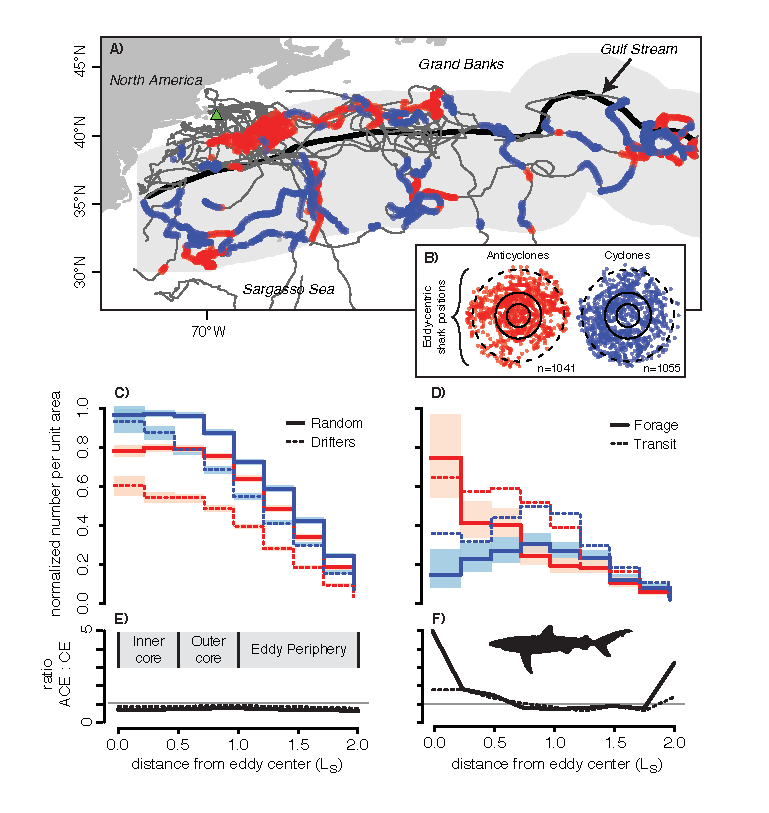
\includegraphics{images/C5_Fig1.pdf}
\caption{Blue sharks tagged in New England frequented the Gulf Stream eddy field (A) and occupied anticyclones (red throughout) and cyclones (blue throughout) at approximately the same frequency (B). Eddy-centric histograms indicated random walk simulations (solid, C) and passive drifters (dashed, C) exhibited higher cyclone use after controlling for eddy area. Sharks (D) used eddy peripheries ($>L_s$) approximately equally between eddies of either polarity, but more positions classified as "transiting" (dashed, D) were collocated around the eddy length scale ($L_s$) compared to "foraging" locations (solid, D). Sharks showed a marked preference for the cores of anticyclones relative to cyclones, particularly while foraging (D). The ratio of anticyclone (ACE) to cyclone (CE) positions across different regions of the eddies are shown for random walk simulations (E), drifters (E) and foraging (solid) and transiting (dashed) modes in the shark data (F). Note confidence intervals have been removed from the transit mode in panel D to aid visualization.}
\label{fig:c5f1}
\end{figure}

\clearpage

%-------------------------

\begin{figure}[htbp]
\centering
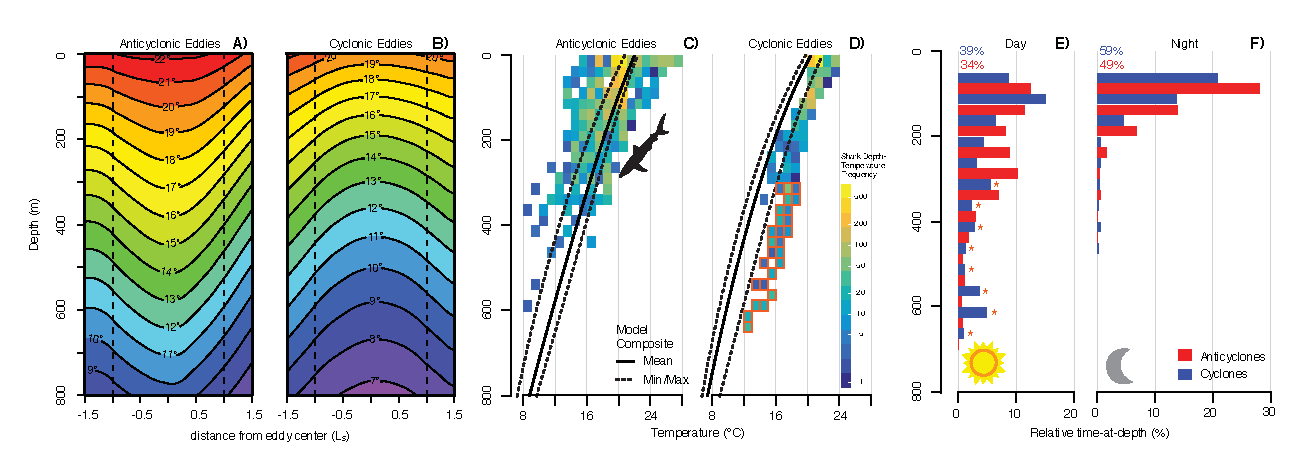
\includegraphics[width=\textwidth]{images/C5_Fig2.pdf}
\caption{Eddy vertical structure and blue shark diving. Modeled depth-temperature profile composites for 27 anticyclonic (A) and 28 cyclonic (B) eddies occupied by blue sharks. Histogram of blue shark depth-temperature data while diving in cores ($r < L_s$) of anticyclones (C; n=7,271) and cyclones (D; n=2,521) compared to model composite depth-temperature profiles. Summary of blue shark time-at-depth during day (E) and night (F) occupation of anticylonic (red) and cyclonic (blue) eddies. The 0-50m depth bin has been removed to aid visualization. The highlighted depth-temperature cells (orange outline, D) and time-at-depth bins (orange asterisks, E) correspond to diving in mode-2 cyclones.}
\label{fig:c5f2}
\end{figure}

\clearpage

%-------------------------

\chapter{Conclusion and Outlook}
\label{chap:6}
\clearpage
\raggedbottom

%\section{Thesis summary and next steps}
% in general, this section should provide some brief synthesis of your work before providing comments on limitations of your work, future directions, questions that arise from your results, etc

%% set the stage: broadly describe in P1 the context within which your thesis operates


%% what does your thesis do? typically you provide ~1 sentence summary of each chapter within a slightly broader narrative of "what it all means". this may be a few paragraphs.


%% in summary, what have we learned from this thesis? what challenges/questions remain?
\section{Summary}

Historically, observing movements of marine fishes has been limited by error in geolocation. These complications have rendered contextualizing observed behaviors and subsequent inference difficult. Consequently, oceanographic associations of many commercially-important or conservation-relevant species remains poorly understood; yet, these animals are immersed in and constantly interacting with a dynamic ocean. In this thesis, I developed a model framework that leverages 3D oceanographic data to improve geolocation error and demonstrated its utility for two species that, historically, have proven challenging to geolocate. This method is poised to leverage future advances as oceanographic data and models continue to improve.

Using the approach I developed and validated in \cref{chap:2}, I applied the model in \cref{chap:3} to study basking sharks in the North Atlantic using a high-resolution oceanographic model. Sharks in this study were tagged around Cape Cod, MA and moved as far as SE Brazil, a total distance of > 17,000 km, and 59\% of tracked individuals exhibited seasonal fidelity to the northeastern US shelf. During these movements, basking sharks made impressive vertical movements to >1,500 m and regularly occupied the mesopelagic, often for months at a time. This study draws attention to the poorly understood ecology of basking sharks and demonstrates the need for international cooperation in managing this highly migratory species that traverses the jurisdictions of dozens of countries each year.

I also applied the model framework from \cref{chap:2} to study the broadbill swordfish (\cref{chap:4}). Due to diel vertical migration and often aphotic behavior, the swordfish has historically proven difficult to study with traditional light-based geolocation. By leveraging significant improvements in geolocation error, I was able to describe mesoscale eddy use by some satellite-tagged individuals in this study. I validated the tag-based observations of eddy use by integrating 2 large fisheries datasets with the independent satellite tag data. Overall, I found swordfish exhibited extreme physiological versatility by occupying a 25$^\circ$C SST range; however, satellite-tagging and fisheries data independently suggested swordfish preferred a much narrower SST range in oligotrophic waters with active front boundaries. Overall, this study makes significant contributions to swordfish ecology and fisheries oceanography by quantifying some of the critical oceanographic influences on swordfish.

In the final data chapter (Chapter \ref{chap:5}), I used the "lessons learned" from the limitations of the previous chapters to design a tagging study to specifically quantify oceanographic associations of blue sharks, as a model pelagic predator. I focused this analysis on the eddy-rich region of the Gulf Stream where I was able to observe blue shark movements and behavior in high-resolution, 3-D as they moved through the eddy field. Using this data, I discovered that blue sharks actively sought the interiors of anticyclonic Gulf Stream eddies. These warm core rings are traditionally characterized as low productivity and anomalously warm, "desert-like" environments. Yet, blue sharks exhibited behaviors indicative of foraging in these features. With high-resolution dive data, I found blue sharks were regularly diving into the mesopelagic during the day in anticyclones, suggesting warm water at depth in these features may alleviate thermal constraints to diving into the mesopelagic to forage. This study provides important insight into the connectivity between epi- and mesopelagic ecosystems and suggests mesopelagic fishes may be a key link between planktonic production and top predators.

%----------------

\section{Outlook}
% limitations/next steps
As with any scientific endeavor, many assumptions were necessary in each of these studies and all left me with more fascinating questions to pursue. The modelling approach developed in \cref{chap:2} was an effective first step at building a flexible, transferable framework that can be readily adapted to animal movement problems in a wide range of taxa and environments. However, many improvements could be implemented, including several provided as feedback from model users. The primary limitations of \texttt{HMMoce} in its original form were its reliance on deprecated, manufacturer-specific software for light-based position estimates as well as support for tags built by a single manufacturer. This was appropriate for our needs, but it was apparent that additional compatibility would be required for widespread adoption of these methods. Further development to incorporate some of these changes are currently underway. In addition, additional process models (\eg including advection) and algorithm support (\eg Viterbi) will dramatically improve utility of this model for the broader community.

While the approach in \cref{chap:3} demonstrated remarkable improvements over previous studies to geolocate a traditionally challenging species, the resulting study was a primarily qualitative depiction of basking shark ecology in the NWA. Future studies could use this or similar datasets to better quantify oceanographic associations, particularly using the high-resolution dive data collected from many of these deployments. In the swordfish analysis in \cref{chap:4}, I was able to quantify habitat use and relate this to oceanography; however, this work would also benefit from further exploration of fine-scale behaviors using the depth-temperature time series from these tags.

Finally, \cref{chap:5} was my attempt to leverage "lessons learned" from the previous chapters to design, fund and conduct a study from end-to-end that would not be constrained by the analytical limitations I faced in previous chapters. While I believe this was largely successful, the high individual variability in eddy use calls for a use-availability control on this data to better quantify blue shark eddy use and identify potential drivers of this behavior. This study would also benefit from incorporating the role of underlying currents, as blue sharks are known to be heavily influenced by advection \citep[\eg][]{Carey1990} and from quantifying fine-scale response to gradients indicative of eddy encounter (\eg sea surface height). These, and other analyses, may aid in further interpretation of the mechanisms driving response of pelagic fishes to mesoscale eddies and their potential functional role(s).



\begin{comment}
%% set the stage: broadly describe in P1 the context within which your thesis operates
%Climate change is arguably one of the most urgent issues presently confronting the world. With no end in sight to the anthropogenic emission of carbon dioxide, expedited warming, sea level rise, and shifts in local and global weather patterns are likely. These changes, however, are not limited to terrestrial ecosystems as coordinated changes in the temperature, carbonate chemistry, stratification, and nutrient environment of the ocean occur. These rapid changes to the Earth's ecosystem highlight the importance of a holistic understanding of the global carbon cycle in which phytoplankton are key players. These climate-related changes to marine ecosystems will likely change the biogeography of phytoplankton as organisms adapt to new environmental conditions. Predicting these changes to the phytoplankton distributions hinges upon understanding the response of phytoplankton both at the community and species-level. In this thesis, I presented new tools (Chapter \ref{chap:2}) and approaches (Chapter \ref{chap:3}-\ref{chap:5}) to survey, characterize, and quantify the response of phytoplankton to changes in their nutrient environment \textit{in situ}. \par

%% what does your thesis do? typically you provide ~1 sentence summary of each chapter within a slightly broader narrative of "what it all means". this may be a few paragraphs.
%This thesis first introduces the development of a statistical approach to identify stably expressed genes for use both in qRT-PCR and metatranscriptomic studies from high-throughput sequencing datasets (Chapter \ref{chap:2}). Many of the ``housekeeping genes'' that are commonly used as references in qRT-PCR studies of phytoplankton were found to be variably expressed across the conditions used in this study. Such variability in a reference gene can drastically alter the gene expression patterns of the gene of interest. This approach broadens the pool of possible gene targets by facilitating the selection of genes without \textit{a priori} knowledge of function. Application of this technique to the metatranscriptomic study in Chapter \ref{chap:3} identified unique stable reference genes for both of the dominant diatoms and facilitated the quantitative comparison of their transcriptional signals. 

%The field study in Narragansett Bay, presented in Chapter \ref{chap:3}, approached the problem of assessing and comparing diatom nutrient physiology in two ways. Metabolic pathways with known relationships to N and P metabolism were tracked for both taxa. This approach suggested that the more dominant \textit{Skeletonema} was likely utilizing inorganic nutrients, where as the less abundant \textit{T. rotula} was relying upon organic compounds, like amino acids. This study, however, went further by combining field samples with incubation experiments. Using a Bayesian approach, these incubation experiments were used to 1) identify novel resource responsive gene targets and 2) contextualize expression signals to directly compare the physiology of organisms \textit{in situ}. This second step was accomplished by proportionalizing the signals in the field to the metabolic bounds on expression observed in the incubation experiments. These data demonstrated significant differences in the expression patterns of resource responsive genes, indicating that these two species are responding differently to the same nutrient environment. Narragansett Bay is an ideal model system for investigating the interplay between diversity and biogeochemistry as well as basic questions in ecology, such as the role of specialization in a dynamic ecosystem. Given the opportunity, I would want to sample this community throughout the year, in combination with similar nutrient experiments that were run for longer duration in larger volumes. While this technique was designed to examine the response of phytoplankton to nutrient dynamics, it could quite easily be expanded to other systems or variables. 

%Chapters \ref{chap:4} and \ref{chap:5}, both set in the oligotrophic North Pacific Subtropical Gyre, look to the opposite ends of the diversity spectrum, assessing the differences in response to nutrient pulse amongst functional groups and amongst strains. By sampling and comparing the global gene expression of the eukaryotic community both \textit{in situ} and in simulated deep seawater (DSW) upwelling incubations, the specific drivers of production for taxonomic groups were identified (Chapter \ref{chap:4}). The divergence in the variable transcript allocation ratio (VTAR) between the diatoms and haptophytes was one of the more surprising outcomes of this study, as it suggests that the r- and K-strategies as defined by enzyme kinetics and growth rate appear to hold true at the level of the transcription. I am quite interested to see if this schism in diatom and haptophyte VTAR is consistent across other stimuli, timescales, and systems\footnote{A preliminary glance at the data from Narragansett Bay suggests that this difference may be upheld.}. In the near future, I would like to replicate this study, with an additional sample 24-hours post-DSW addition in order to assess the more immediate response of the community to nutrient addition, potentially removing the signals associated with shifts in the community structure. 

%The other rather perplexing outcome from this study was the lack of response seen in the dinoflagellates following DSW addition. Chapter \ref{chap:4} suggests that this might be due to the fact that dinoflagellates might have alternative trophic strategies or live symbiotically. However, I suspect that that it is more of a general characteristic of dinoflagellate transcriptional regulation, or, rather, the lack thereof. It is known that autotrophic dinoflagellates do respond at the protein and activity level to changes in their nutrient environment \citep{Dyhrman1999}. Though not discussed in this thesis, expression patterns of \textit{Prorocentrum} in the Narragansett Bay incubations suggest that this pattern of no regulation may hold true in coastal dinoflagellates as well. Together, these data seem to indicate that metabolic plasticity in the dinoflagellates is happening at the protein level. It remains to be seen if these general patterns are upheld in future transcriptomic and metatranscripomic studies. 

%Finally, Chapter \ref{chap:5} investigates the intersecting roles of metabolic plasticity and strain diversity in the response of the \textit{Emiliania huxleyi} species complex to changing nutrient environments. The co-existence of at least five strains was observed in the environment, as defined by the variable gene sets. Additionally, following the addition of N, the strain composition of the field appeared to be altered. These findings support the hypothesis of \citet{Read2013} that the variability in gene content as observed in the pan genome is present and modulated in the field. Additionally, metabolic plasticity, as defined by changes in transcript abundance, was observed, particularly in metabolic processes associated with N and P metabolism, as well as life stage and calcification. The fact that any genes were identified as significantly differentially regulated in this study is surprising, as the two ``biological replicates'' used were actually distinct incubation experiments that were performed approximately two weeks apart with different initial populations. This, combined with the fact that many of these gene targets were also identified as significantly differentially regulated in N and P limited cultures in proteomic work by \citet{McKew2015}, suggests that these responses to nutrient stress are highly conserved within the \textit{E. huxleyi} species consortium. In my opinion this study highlights the importance of culturing diversity. In many ways, even with metatranscriptome assembly, we are limited by what we know; our ability to assign function or taxonomy to meta-omic data in the field hinges upon our databases. 

%% in summary, what have we learned from this thesis? what challenges/questions remain?
%Together these data provide new insights into the inner workings of the phytoplankton consortia, illuminating potentially missed co-limitations, capabilities, and interactions. Yet, the ultimate fate of these data beyond my very narrow field remains uncertain. Currently there is a disconnect between the type of data that we biologists want to collect and the type of data that ecosystem and ocean modelers want. The undertone of some of the chapters in this thesis is that these findings might be integrated into biogeochemical models. While I do believe that progress is being made toward this ultimate goal\footnote{In particular, the Darwin Project \citep{Follows2007} and some interesting, as of yet unpublished, work by Victoria Coles are pushing the boundaries on this integration.}, many hurdles remain \citep{Hood2007, Worden2015}. With continued collaboration and discourse between molecular ecologists and ecosystem modelers, I am hopeful that a solid quantitative connection might be made. 



\end{comment}
\appendix
%\renewcommand{\thefigure}{\Alph{chapter}.\arabic{figure}}
\renewcommand{\thetable}{\Alph{chapter}-\arabic{table}}
\chapter{Supplemental Information}

\raggedbottom


%%%%%%%%%%%%%%%%%%%%%%%%%%%

%%%%%%%%%%%%%%%%%%%%%%%%%%%_________________CHAPTERTWO_________________%%%%%%%%%%%%%%%%%%%%%%%%%%%

%%%%%%%%%%%%%%%%%%%%%%%%%%%
\clearpage
\section{Appendix for Chapter 2}
\subsection{Supplemental Figures}
%Supplemental Figure 1: Histogram of TPM distribution
\begin{figure}[h!]
  \centering
    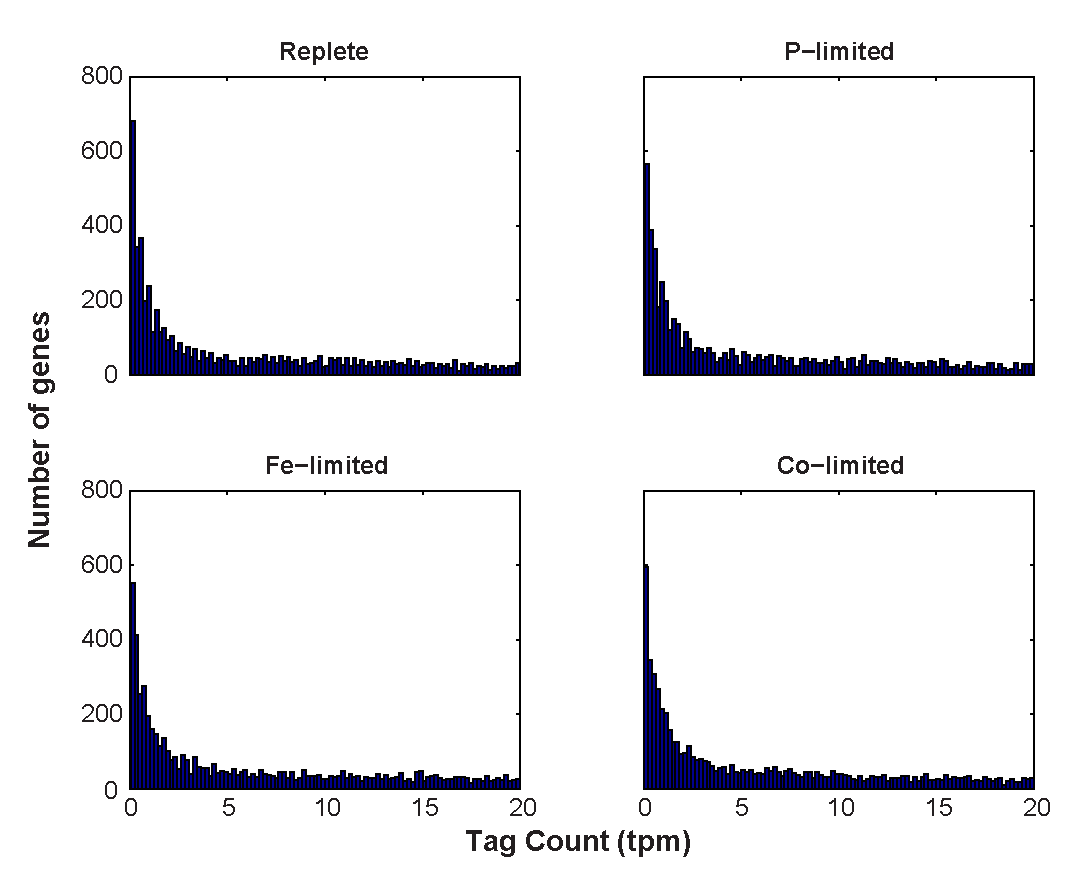
\includegraphics[width=1\textwidth]{Images/C2_FigureS1_v6.pdf}
    \caption[Distribution of normalized tag counts across treatments]{Histogram analysis of the distribution of normalized tag counts (TPM) for each gene across each of the four treatments (Replete, P-limited, Fe-limited, and co-limited). The abundance of normalized tag counts (TPM) was assessed, tallying the total number of genes with a given tag count. Only tag counts less than 20 are depicted to aid the visualization of the inflection in the data at 2.5 TPM.}
  \label{fig:a1f1}
\end{figure}

%Supplemental Figure 2: K-means clusters (all)
\begin{landscape}
   \null         %%<---- this is needed
   \vfill        %%<-----here
   \centering 
    \begin{figure}
    \centering
        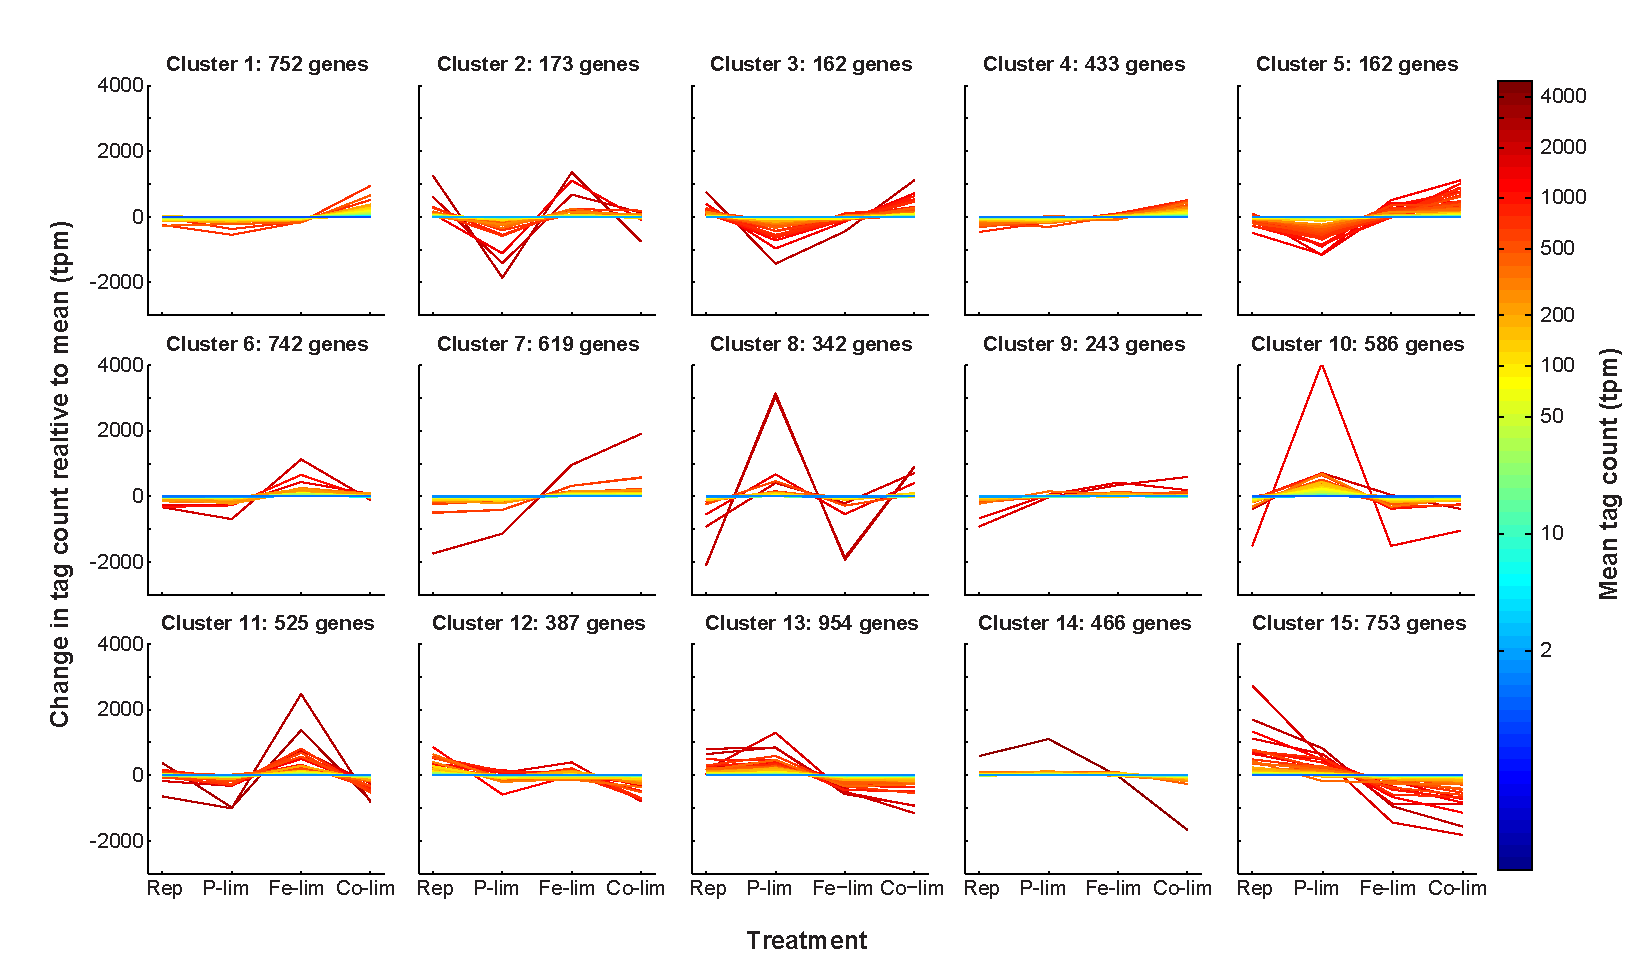
\includegraphics[width=1\textwidth]{Images/C2_FigureS2_v6.pdf}
        \caption[$K$-means clustering of normalized genes]{$K$-means clustering of normalized genes. The 7380 genes that passed the 2.5 TPM cutoff were clustered into 15 clusters using the $k$-means algorithm under the Pearson correlation coefficient. Tag counts normalized to total library size (in TPM) for each gene are plotted relative to the mean (indicated by the color of the line) for each of the four treatments: Replete (Rep), P-limited (P-lim), Fe-limited (Fe-lim), and co-limited (Co-lim).}
    \label{fig:a1f2} 
    \end{figure}
    \vfill        %%<----- and here
\end{landscape}

\clearpage
\newpage

%%%%%%%%%%%%%%%%%%%%%%%%%%%

%%%%%%%%%%%%%%%%%%%%%%%%%%%_________________CHAPTERTHREE_________________%%%%%%%%%%%%%%%%%%%%%%%%%%%

%%%%%%%%%%%%%%%%%%%%%%%%%%%


\section{Appendix for Chapter 3}
\subsection{Supplemental Figures}

%Supplemental Figure 1: Cell counts in NB 
\begin{figure}[h!]
  \centering
    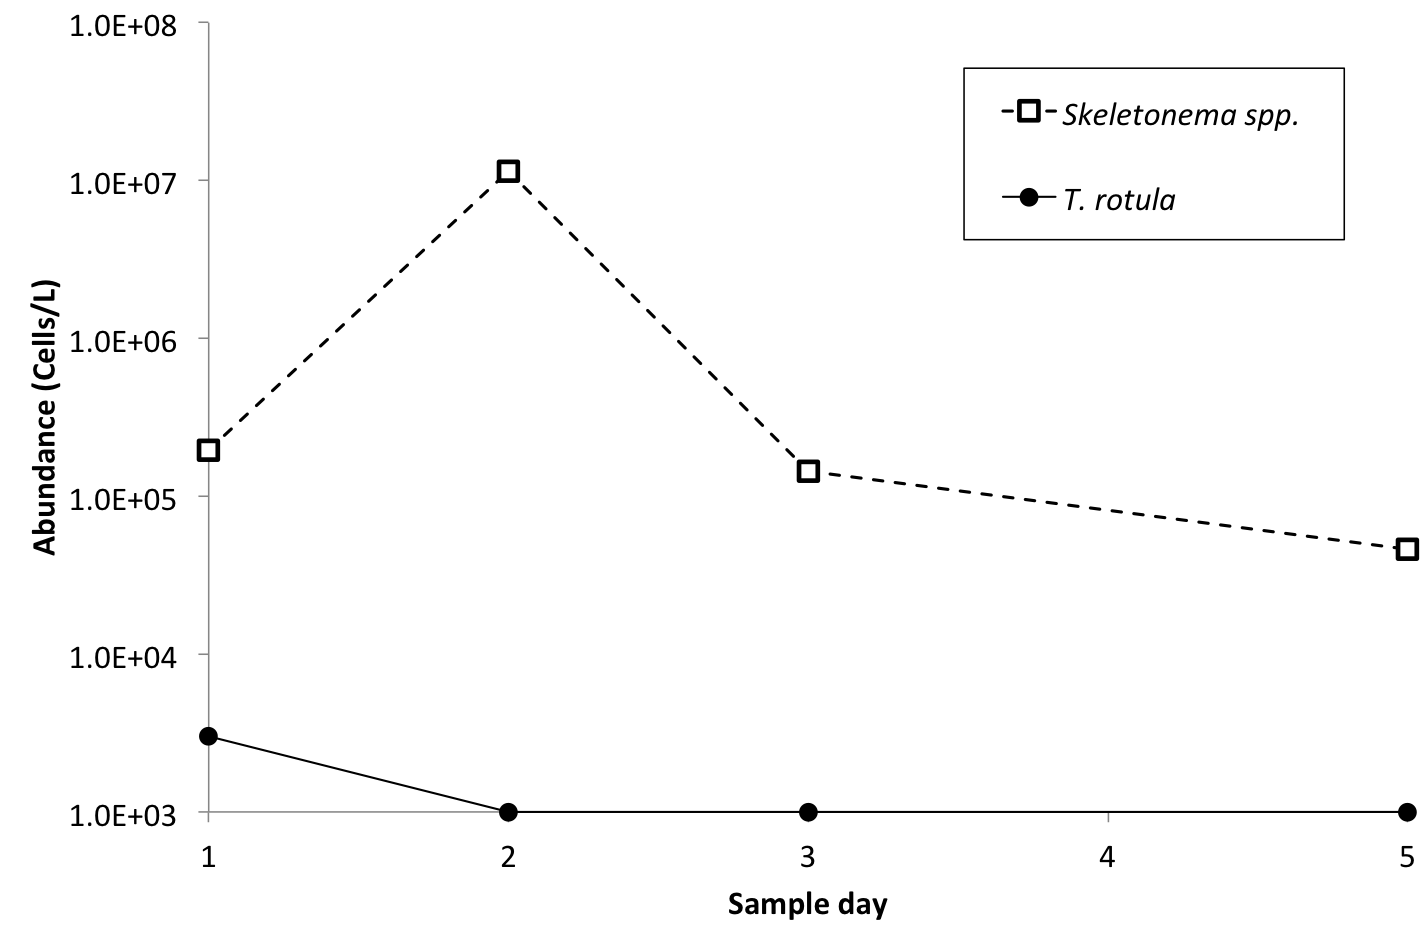
\includegraphics[width=1\textwidth]{Images/C3_SFigure1_CellCounts.png}
    \caption[Cell counts in Narragansett Bay during the spring of 2012]{Abundance estimation from cell counts of \textit{Skeletonema} spp. and \textit{T. rotula} across the five sample points during the spring of 2012. }
  \label{fig:a3f1}
\end{figure}


%Supplemental Figure 2: KEGG linear correlation
\begin{figure}[p!]
  \centering
    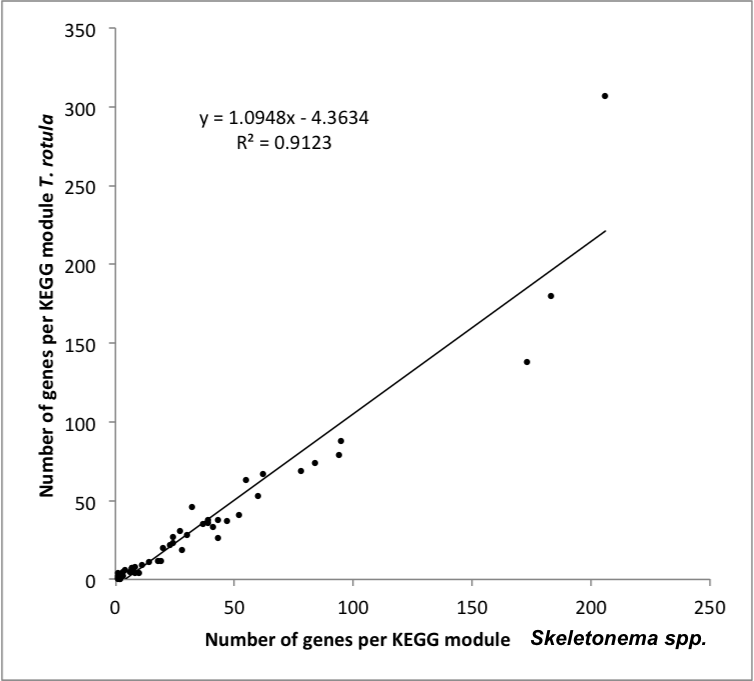
\includegraphics[width=1\textwidth]{Images/C3_SFigure2_KEGGModuleGeneContent2.png}
    \caption[Comparison of KEGG module content between \textit{Skeletonema} spp. and \textit{T. rotula} ]{Total number of genes assigned to each KEGG module for \textit{Skeletonema} spp. and \textit{T. rotula}.}
  \label{fig:a3f2}
\end{figure}


%Supplemental Figure 3: Hierarchical clustering of S and T across time
\begin{figure}[p!]
  \centering
    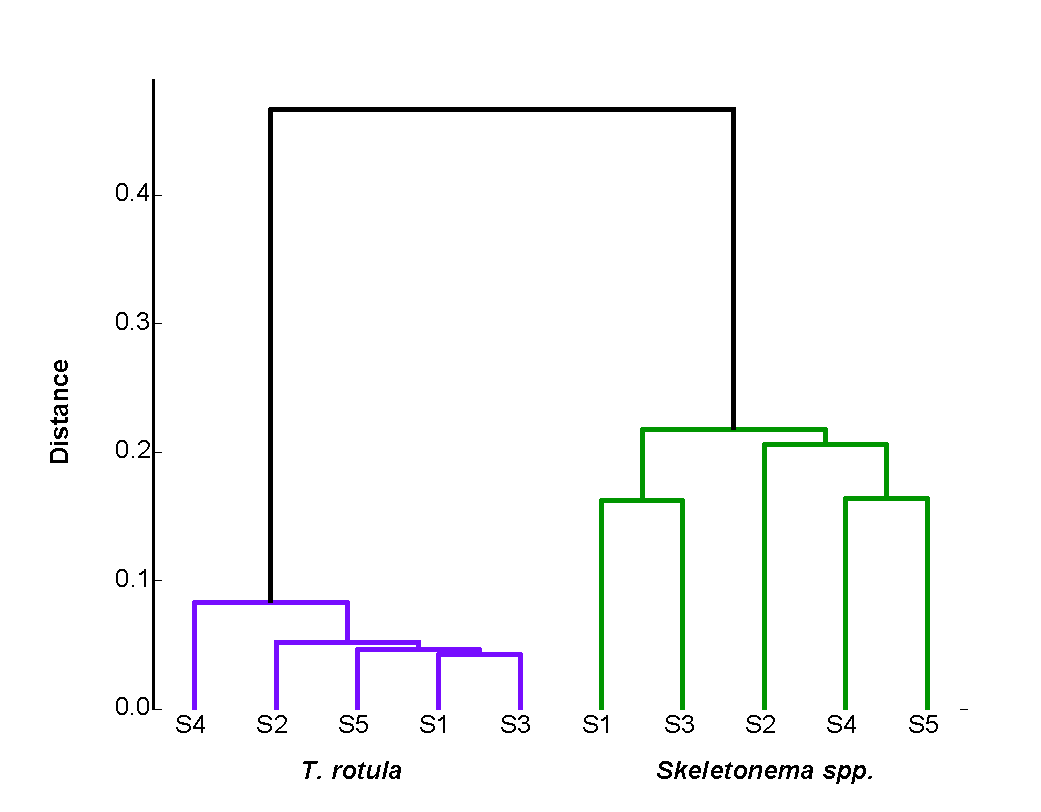
\includegraphics[width=1\textwidth]{Images/C3_SFigure3_Dendrogram.pdf}
    \caption[Hierarchical clustering of QMF signatures across species and samples]{Dendrogram depicting hierarchical clustering of samples based on relative expression of KEGG modules (Figure 2) across the five samples S1-S5 for \textit{Skeletonema} spp. and \textit{T. rotula}.}
  \label{fig:a3f3}
\end{figure}

%Supplemental Figure 4: Stable gene expression across time
\begin{figure}[p!]
  \centering
    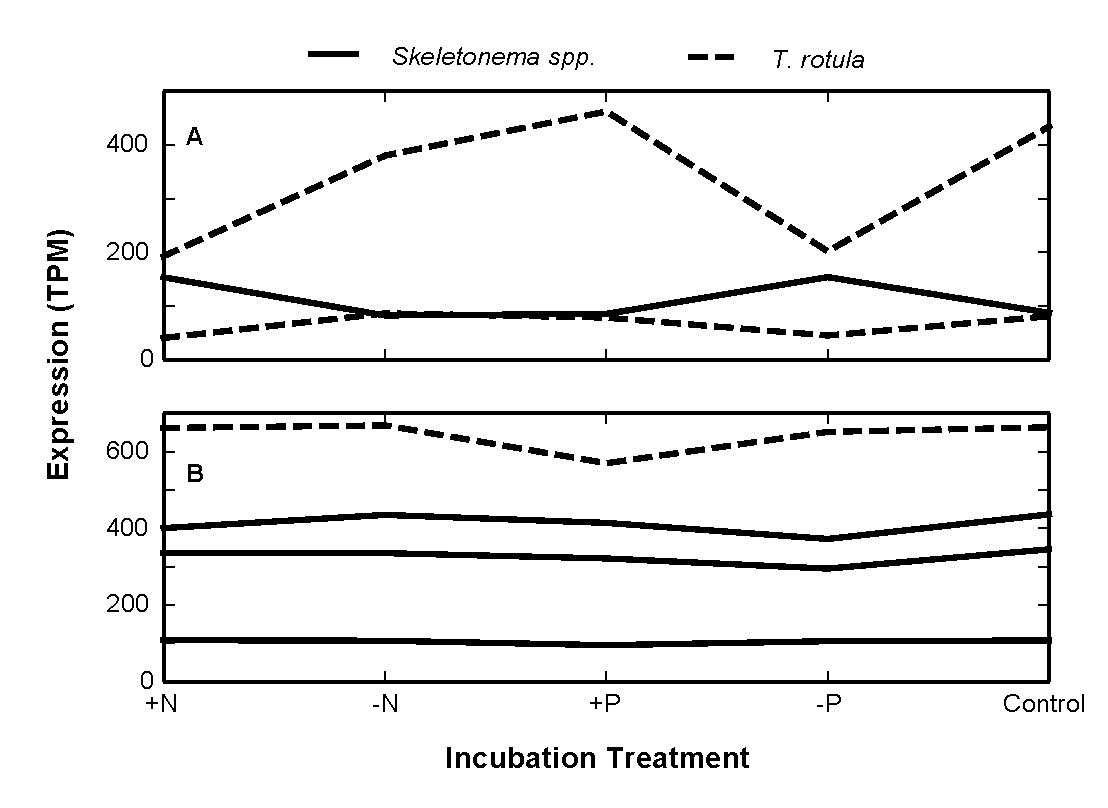
\includegraphics[width=1\textwidth]{Images/C3_SFigure4_StableGenePlot_wActin.pdf}
    \caption[Expression of stable reference genes in the field]{Expression of stable reference genes identified based on literature and statistical parsing in nutrient amendment incubation. (A) The expression in tags per million ($TPM$) of stable reference genes identified in \textit{T. rotula} (dashed line) and \textit{Skeletonema} spp.  (solid lines) based on homology (e-value < 1e-5) to a known reference genes in \textit{T. pseudonana}, ACT1 (Thaps\_25772), in nutrient incubations. (B) Also shown are reference genes identified in the incubation experiments, using statistical analysis of sequence counts \citep{Alexander2012, Wu2010}, and nutrient incubations }
  \label{fig:a3f4}
\end{figure}

%Supplemental Figure 5: RR gene composition
\begin{figure}[p!]
  \centering
    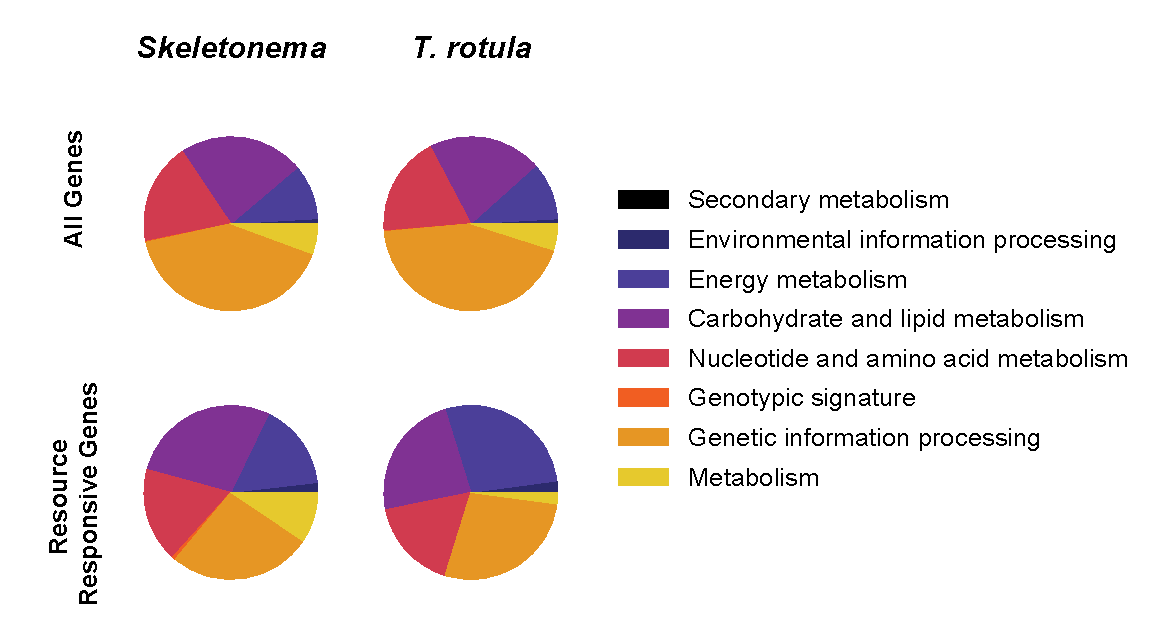
\includegraphics[width=1\textwidth]{Images/C3_SFigure5_RR_All_Genes_Pie.pdf}
    \caption[Functional compoosition of the reference transcriptome and resource-responsive gene sets]{Functional composition of the reference transcriptome and resource-responsive (RR) gene subset for \textit{T. rotula} and \textit{Skeletonema} spp. (A) RR gene sets were identified through cross comparison of like-nutrient incubations (i.e. +N vs. -N and +P vs. -P), using ASC (fold change = 2, post-$p > 0.95$). The relative functional categorization of the reference transcriptomes and RR gene set for \textit{T. rotula} and \textit{Skeletonema} spp. based on KEGG ontology as assigned by KAAS is depicted at the module-level.}
  \label{fig:a3f5}
\end{figure}

%Supplemental Figure 6: Expression of nitrate reductase

\begin{figure}[p!]
  \centering
    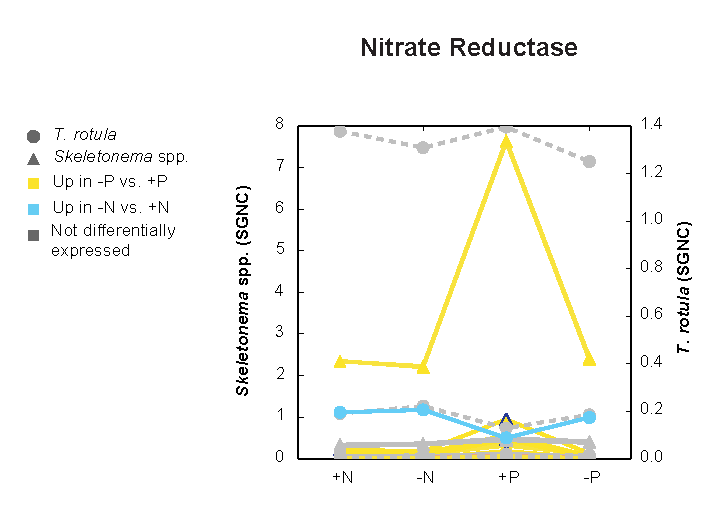
\includegraphics[width=1\textwidth]{Images/C3_SFigure6_SGNC_NitrateReductase.pdf}
    \caption[Relative expression of nitrate reducatses across incubation experiments]{The relative expression in stable gene normalized counts ($SGNC$) of the assimilatory nitrate reductase gene cluster across the incubation experiment treatments. Significance of regulation between the treatments is denoted by the color of the line; organisms are denoted by the shapes of the marker.}
  \label{fig:a3f6}
\end{figure}

%Supplemental Figure 7: Cluster Analysis


\begin{figure}[p!]
  \centering
    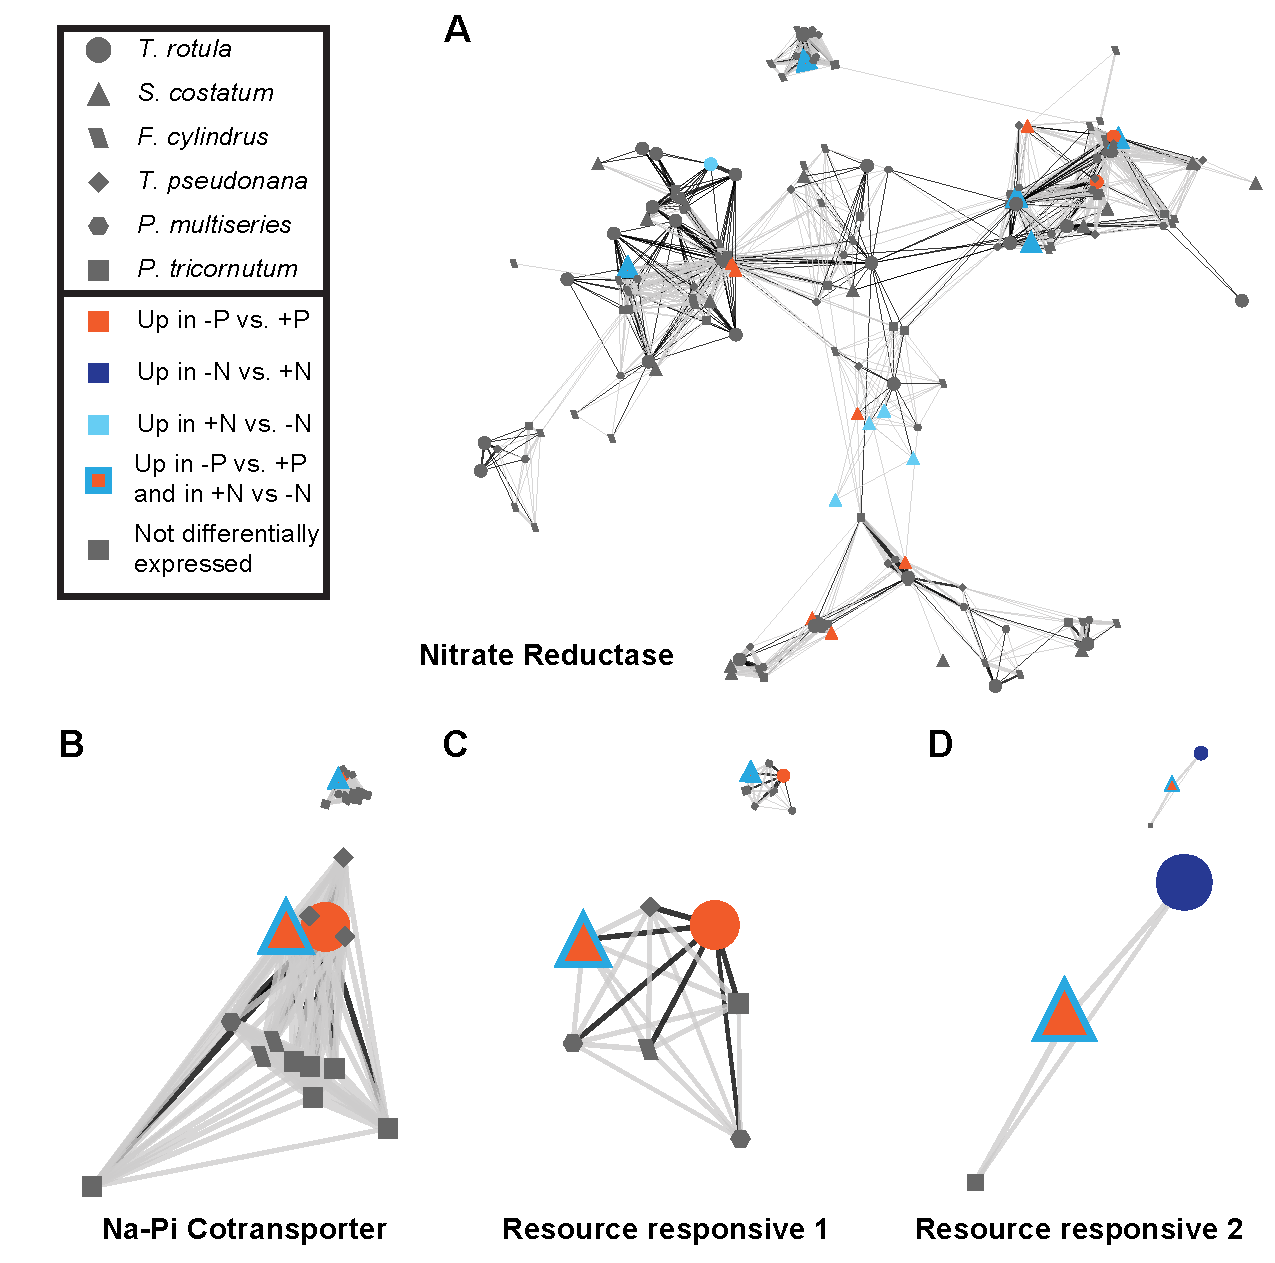
\includegraphics[width=1\textwidth]{Images/C3_SFigure7_ClusterAnalysis_v5.pdf}
    \caption[Gene cluster analysis of nutrient-responsive genes]{Gene cluster known nutrient-responsive genes in \textit{T. pseudonana}: (A) assimilatory nitrate reductase and (B) sodium-phosphate cotransporter and novel resource-responsive (RR) gene families: (C) RR1 and (D) RR2. Transcripts from the transcriptomes of \textit{T. rotula} and \textit{Skeletonema} spp. were clustered based upon relative homology with available diatom genomes: \textit{F. cylindrus}, \textit{P. tricornitum}, \textit{P. multiseries}, and \textit{T. pseudonana}. Symbols indicate different species, while color indicates regulation in the field incubation experiments. Two nodes within a gene cluster are connected by an edge if they share a homologous protein (reciprocal BLAST hit with a minimum of 1e-5 score and minimum 20\% identity). Gene clusters are visualized using an edge-weighted spring-embedded model based on e-value, meaning that genes that are closer together are more similar. The width of the line correlates to the magnitude of the e-value, with lower e-values represented by thicker lines and higher e-values represented by thinner lines.}
  \label{fig:a3f7}
\end{figure}

%Supplemental Figure 8: Conceptual schematic of STD niche space

\begin{figure}[p!]
  \centering
    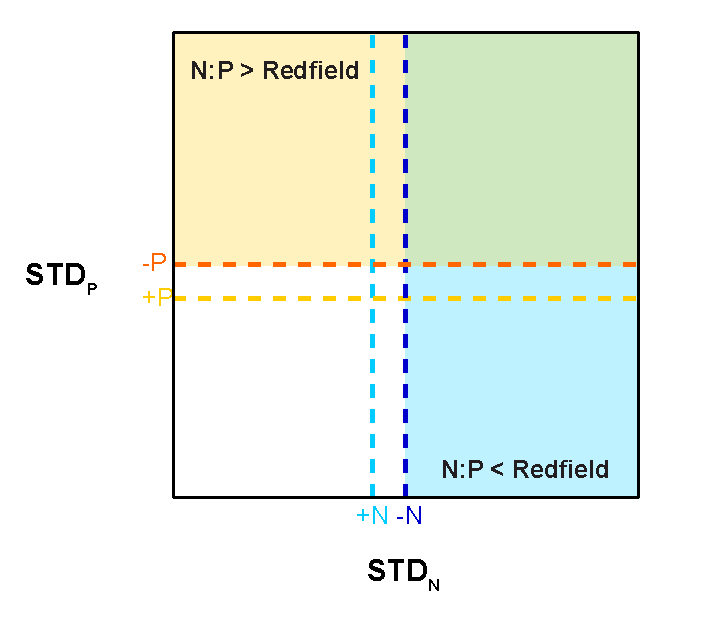
\includegraphics[width=1\textwidth]{Images/C3_SFigure8_Schematic_Quadrants.pdf}
    \caption[Conceptual schemiatic of $STD_N$ plotted against $STD_P$]{A conceptual schematic of $STD_N$ plotted against $STD_P$ hypothesized regions of N:P > Redfield physiology and N:P < Redfield physiology highlighted.}
  \label{fig:a3f8}
\end{figure}


%Supplemental Figure 9: NISP Dn genes
\begin{landscape}
   \centering
   \null         %%<---- this is needed
   \vfill        %%<-----here

	\begin{figure}
  	\centering
    	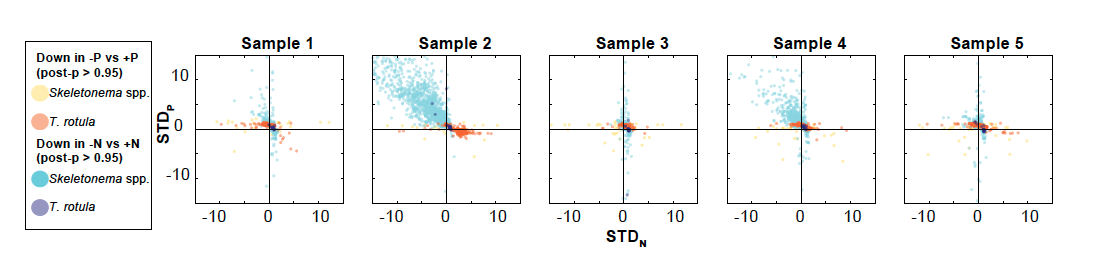
\includegraphics[width=1.3\textwidth]{Images/C3_SFigure9_NISP_DNGenes.png}
    	\caption[Evolution of niche space indexing over for significantly down-regualted genes]{Evolution of niche space indexing over time in Narragansett Bay for \textit{T. rotula} and \textit{Skeletonema} spp.. The stable gene normalized field signal from genes identified as significantly (2-fold change, post$-p > 0.95$) down-regulated in -P vs +P for Skeletonema spp. (yellow) and \textit{T. rotula} (orange) and in -N vs +N for for \textit{Skeletonema} spp. (cyan) and \textit{T. rotula} (dark blue) was proportionalized relative to the expression for those genes in nutrient incubations, yielding the $STD_N$ and $STD_P$. These data are plotted for Sample 1 through Sample 5.}
  	\label{fig:a3f9}
	\end{figure}
    \vfill        %%<----- and here
\end{landscape}

%Supplemental Figure 10: Percentage of RR genes by quadrant

\begin{figure}[h!]
  \centering
    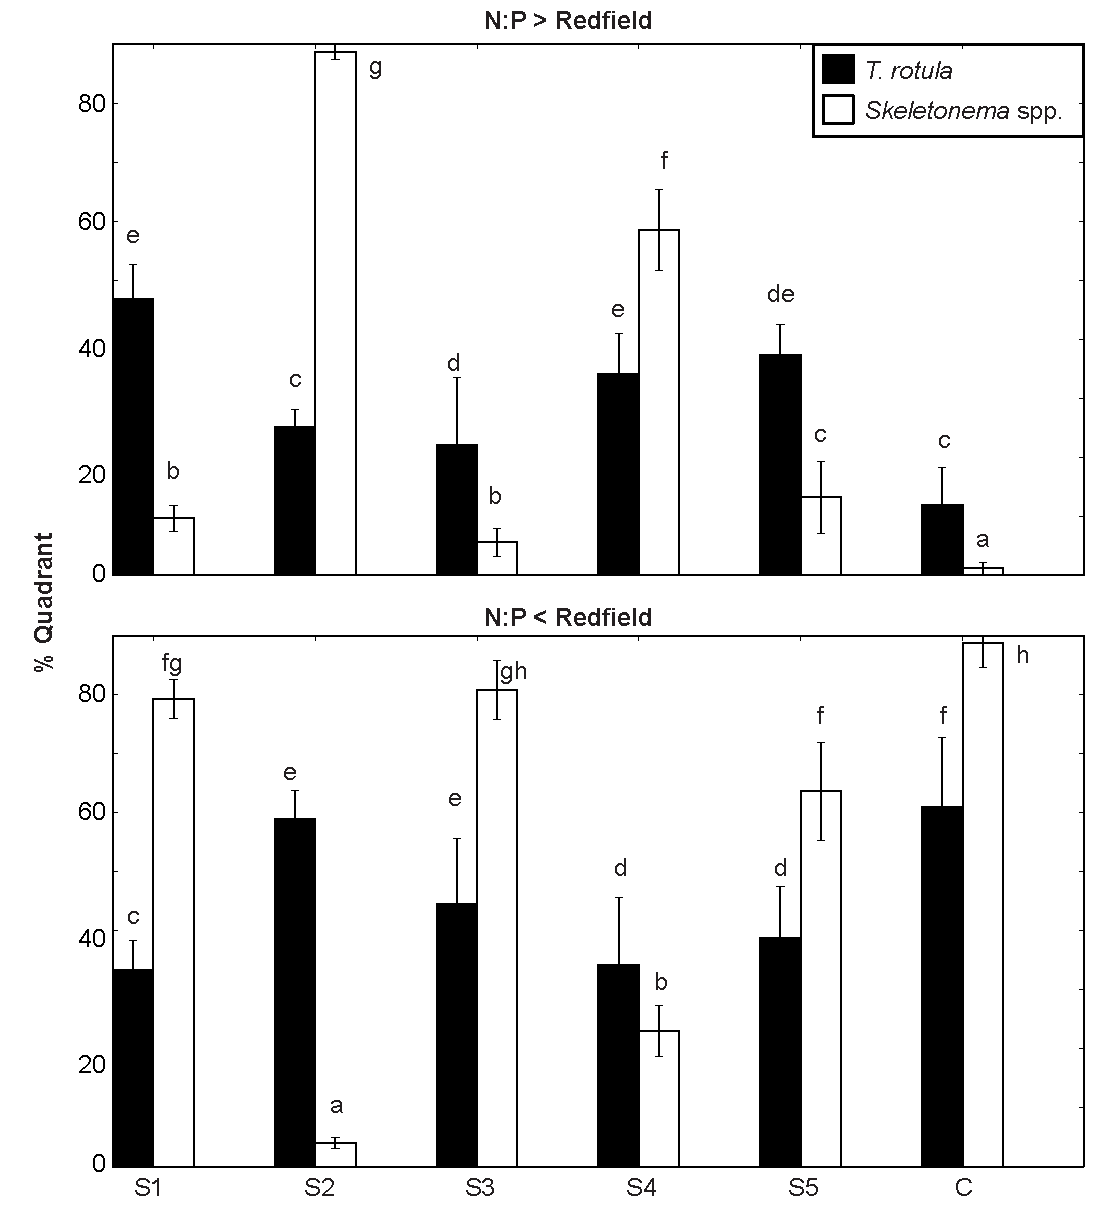
\includegraphics[width=1\textwidth]{Images/C3_SFigure10_BarGraph_Quadrant_2575_stats.pdf}
    \caption[The percentage of identified nutrient responsive genes falling into the N:P > Redfield and N:P < Redfield quadrants with varried cutoffs]{The percentage of identified nutrient responsive genes falling into the N:P > Redfield and N:P < Redfield quadrants for \textit{T. rotula} and \textit{Skeletonema} spp.. The total number of genes falling into the N:P > Redfield quadrant ($STD_P > C$; $STD_N < C$, for $0.25 < C < 0.75$) and the N:P < Redfield quadrant ($STD_P$ < C; $STD_N > C$, for $0.25 < C < 0.75$). The value of C was varied over 10 different values and the average percentages of genes falling into each of the quadrants is depicted above based on the size of the circle at the median $STD_N$ and $STD_P$ for the genes in the quadrant. Similarity of data between species by quadrant was assessed using an analysis of variance (ANOVA) with a generalized linear model. The results from a post hoc Tukey test show the divergence of species across time ($p < 0.05$).}
  \label{fig:a3f10}
\end{figure}

%Supplemental Figure 11: Quadrant localization with varying stable reference genes

\begin{figure}[p!]
  \centering
    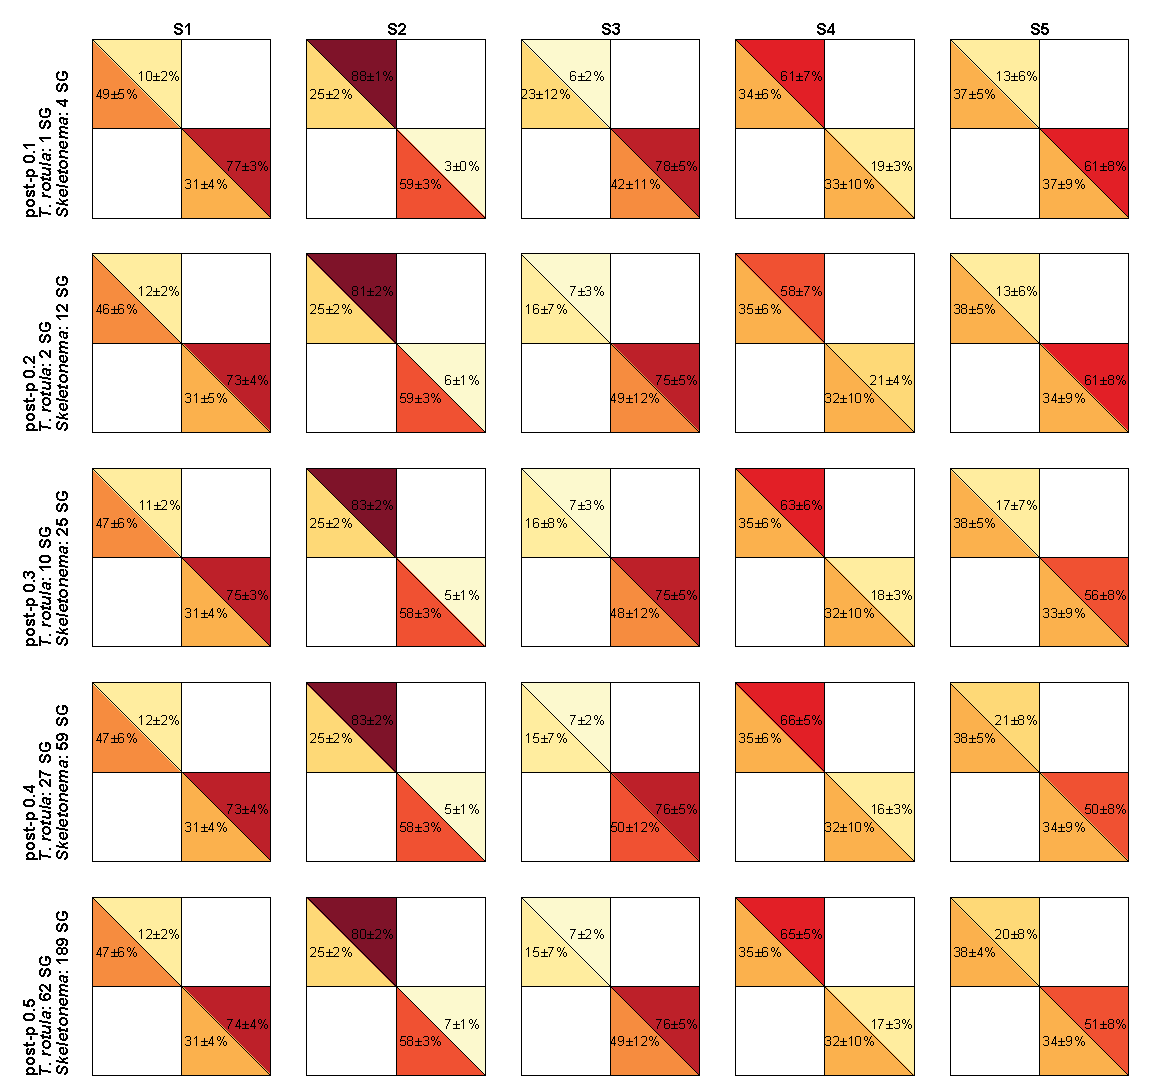
\includegraphics[width=1\textwidth]{Images/C3_SFigure11_Quadrant.pdf}
    \caption[The impact of stable gene selction of quadrant localization]{The impact of stable gene selection on the quadrant localization of the resource responsive gene sets. The posterior probability cutoff used in the selection of stable genes was varied from 0.1 to 0.5 for a fold change of 1.25. The percentage of identified nutrient responsive genes falling into the N:P > Redfield and N:P < Redfield quadrants for \textit{T. rotula} and \textit{Skeletonema} spp. across the five sample points and five posterior probability values is depicted.}
  \label{fig:a3f11}
\end{figure}



\subsection{Supplemental Tables}

%Supplemental Table 1: library stats

\begin{table}[h!]
\centering
\caption[The total number of paired end reads after quality control and trimming and the percentage of reads mapping]{The total number of paired end reads after quality control and trimming and the percentage of reads mapping to the \textit{T. pseudonana} genome, \textit{T. rotula} transcriptome, and \textit{S. costatum} transcriptome.}
\label{tab:a3t1}

\newcolumntype{C}[1]{>{\centering\let\newline\\\arraybackslash\hspace{.5pt}}m{#1}}

\begin{tabular}{|C{2cm}|C{2.5cm}|C{2.5cm}|C{2.5cm}|C{2.5cm}|}
\hline
\multirow{2}{*}{Sample} & \multirow{2}{*}{\parbox{2.5cm}{Total library size (paired end reads)}} & \multicolumn{3}{c|}{Mapped representation in library} \\ \cline{3-5} 
                        &                                                              & \textit{T. pseudonana}      & \textit{T. rotula}      & \textit{S. costatum}     \\ \hline
S1                      & 89455034                                                     & 2.98\%             & 17.50\%        & 33.50\%         \\ \hline
S2                      & 64888267                                                     & 0.41\%             & 11.70\%        & 54.90\%         \\ \hline
S3                      & 103250243                                                    & 0.39\%             & 7.30\%         & 9.00\%          \\ \hline
S4                      & 45370867                                                     & 0.68\%             & 8.80\%         & 8.30\%          \\ \hline
S5                      & 55061692                                                     & 0.88\%             & 10.40\%        & 11.20\%         \\ \hline
Ambient Control         & 51508197                                                     & 0.27\%             & 13.40\%        & 8.00\%          \\ \hline
+N                      & 58626239                                                     & 0.43\%             & 6.10\%         & 5.30\%          \\ \hline
-N                      & 44561851                                                     & 0.41\%             & 8.70\%         & 8.30\%          \\ \hline
+P                      & 51130364                                                     & 0.29\%             & 8.50\%         & 8.00\%          \\ \hline
-P                      & 58834022                                                     & 0.40\%             & 6.60\%         & 6.50\%          \\ \hline
\end{tabular}
\end{table}

%Supplememntal Table 2: nutrient concentrations used in incubations

\begin{table}[h!]
\centering
\caption[Nutrient concentrations used in nutrient amendment incubations. ]{Nutrient concentrations used in nutrient amendment incubations.}
\label{tab:a3t2}
\begin{tabular}{|c|c|c|c|c|c|}
\hline
                                    & \multicolumn{5}{c|}{\textbf{Treatment}}                                                                                              \\ \cline{2-6} 
\multirow{-2}{*}{\textbf{Nutrient}} & Ambient Control          & + P                      & + N                      & - P                      & - N                      \\ \hline
Nitrate                             & \cellcolor[HTML]{C0C0C0} & \cellcolor[HTML]{C0C0C0} & 10 $\mu M$                    & 10 $\mu M$                    & \cellcolor[HTML]{C0C0C0} \\ \hline
Phosphate                           & \cellcolor[HTML]{C0C0C0} & 3 $\mu M$                     & \cellcolor[HTML]{C0C0C0} & \cellcolor[HTML]{C0C0C0} & 3 $\mu M$                     \\ \hline
Silica                             & \cellcolor[HTML]{C0C0C0} & \cellcolor[HTML]{C0C0C0} & \cellcolor[HTML]{C0C0C0} & 68 $\mu M$                    & 68 $\mu M$                    \\ \hline
Iron                                & \cellcolor[HTML]{C0C0C0} & \cellcolor[HTML]{C0C0C0} & \cellcolor[HTML]{C0C0C0} & 4.6 $\mu M$                   & 4.6 $\mu M$                   \\ \hline
Vitamins                            & \cellcolor[HTML]{C0C0C0} & \cellcolor[HTML]{C0C0C0} & \cellcolor[HTML]{C0C0C0} & f/5                      & f/5                      \\ \hline
\end{tabular}
\end{table}


%Supplememntal Table 3: nutrient concentrations used in incubations

\begin{table}[h!]
\centering
\caption[Mapping statistics for \textit{T. rotula} and \textit{S. costatum} transcriptomes]{Total number of contigs in the \textit{T. rotula} and \textit{S. costatum} transcriptomes and the number of genes in each of the differentially regulated and stable groupings.}
\label{tab:a3t3}
\begin{tabular}{|l|l|l|}
\hline
                                                                       & \textit{\textbf{T. rotula}} & \textit{\textbf{S. costatum}} \\ \hline
Number of contigs in transcriptome                                     & 22362                       & 27665                         \\ \hline
Pass 2 TPM cutoff                                                      & 4318                        & 20921                         \\ \hline
Up in -P vs +P                                                         & 249                         & 4754                          \\ \hline
Down in -P vs +P                                                       & 335                         & 52                            \\ \hline
Up in -N vs +N                                                         & 196                         & 9                             \\ \hline
Down in -N vs +N                                                       & 49                          & 1631                          \\ \hline
All differentially regulated (2 fold change, post-$p > 0.95$) & 775                         & 5136                          \\ \hline
Stable genes (1.25 fold change, post-$p < 0.1$)                  & 1                           & 4                             \\ \hline
\end{tabular}
\end{table}




%%%%%%%%%%%%%%%%%%%%%%%%%%%

%%%%%%%%%%%%%%%%%%%%%%%%%%%_________________CHAPTERFOUR_________________%%%%%%%%%%%%%%%%%%%%%%%%%%%

%%%%%%%%%%%%%%%%%%%%%%%%%%%


\clearpage

\section{Appendix for Chapter 4}
\subsection{Supplemental Figures}

%Supplemental Figure 1: Chlorophyll values in experiments and in situ samples 
\begin{figure}[h!]
  \centering
    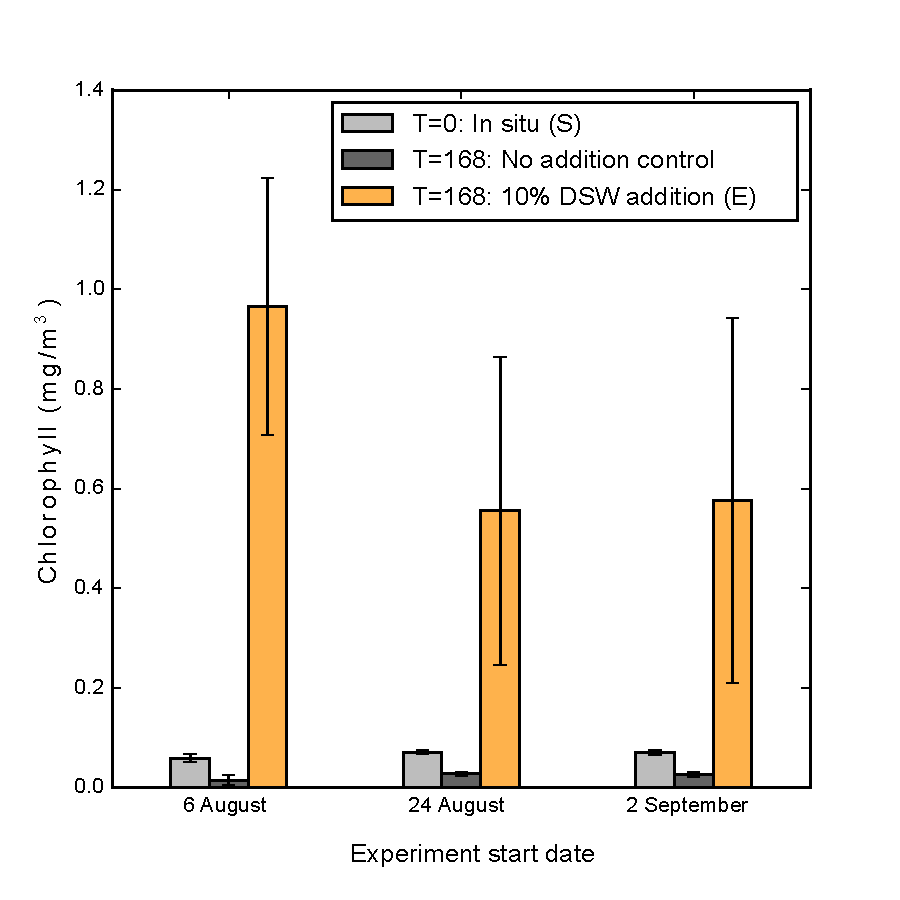
\includegraphics[width=1\textwidth]{Images/C4_FigureS1.pdf}
    \caption[Chlorophyll a of replicated experiments for \emph{in situ} samples, no addition control, and a 10\% deep seawater amendment]{Chlorophyll a of replicated experiments for \emph{in situ} samples (S), a no addition control, and a 10\% deep seawater (DSW) amendment (E). Incubation samples were harvested after 168 hours.}
  \label{fig:a4f1}
\end{figure}


%Supplemental Figure 2: Rank abundance shifts in species composition of diatoms, haptophytes and dinoflagellates

\begin{figure}[p!]
  \centering
    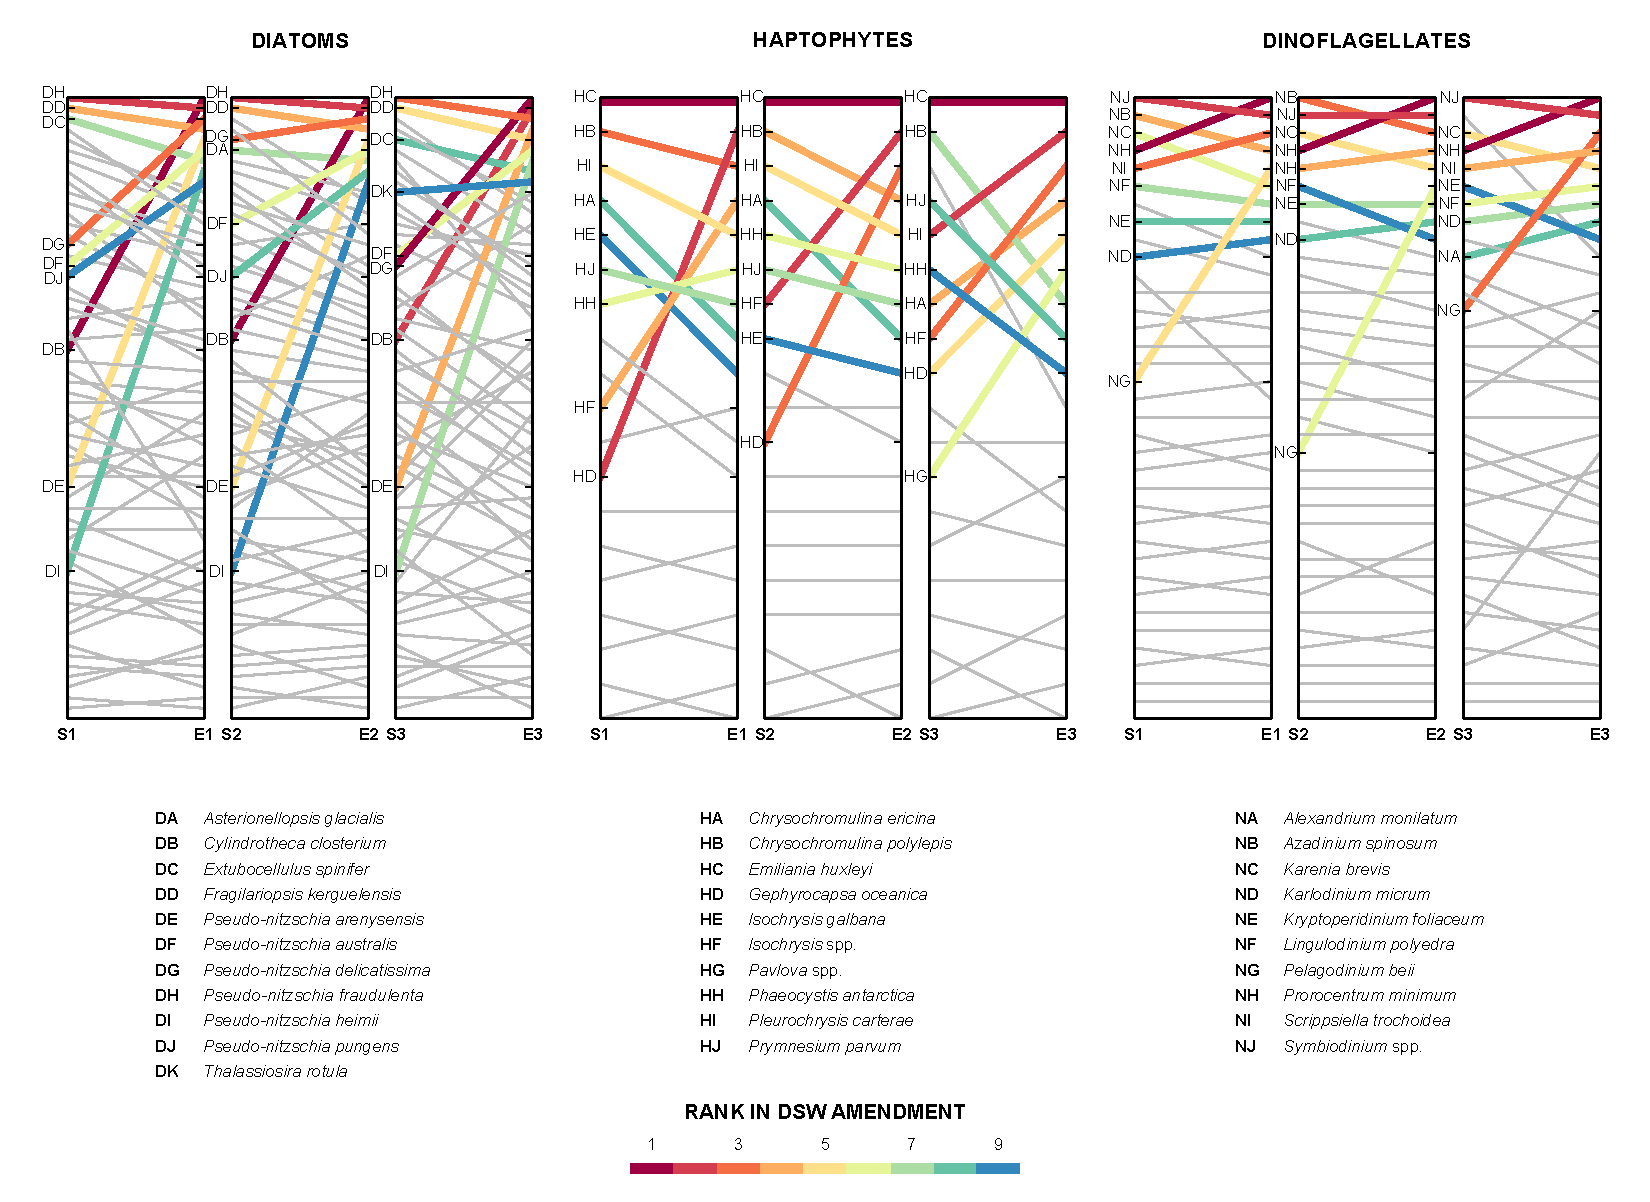
\includegraphics[width=1\textwidth]{Images/C4_FigureS2.pdf}
    \caption[Rank abundance shifts in the species composition of diatoms, haptophytes and dinoflagellates]{Rank abundance shifts in the species composition of diatoms, haptophytes and dinoflagellates for the three experiments. The relative shift in rank abundance for each species is depicted for each incubation experiment (E1-E3) following deep seawater (DSW) addition. The nine most abundant taxa following DSW addition are highlighted for each of the functional groups. Although the species that recruited the reads are denoted here this is highly driven by the composition of the database and does not necessarily indicate the actual species present, but rather the closest species present in the database.}
  \label{fig:a4f2}
\end{figure}

%Supplemental Figure 3: QMF Comparison across species


\begin{figure}[p!]
  \centering
    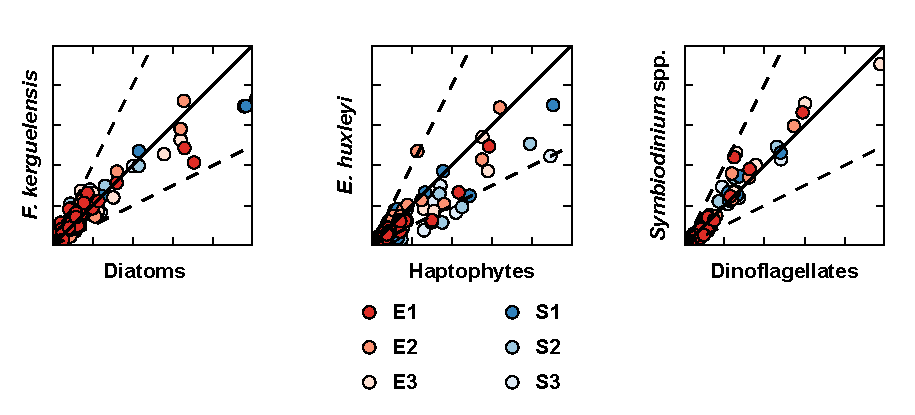
\includegraphics[width=1\textwidth]{Images/C4_FigureS3.pdf}
    \caption[Comparison of the quantitative metabolic fingerprint (QMF) between the whole functional group and representative taxa]{Comparison of the quantitative metabolic fingerprint (QMF) between the whole functional group and representative taxa. The proportion of reads falling into each of the modules depicted in Figure 2 is plotted for S1-S3 and E1-E3, comparing the summed functional group signal and that of a representative taxon. Color of the marker indicates the sample; solid and dashed lines mark the 1:1 and 1:2 lines, respectively.}
  \label{fig:a4f3}
\end{figure}

%Supplemental Figure 4: Distribution histogram

\begin{figure}[p!]
  \centering
    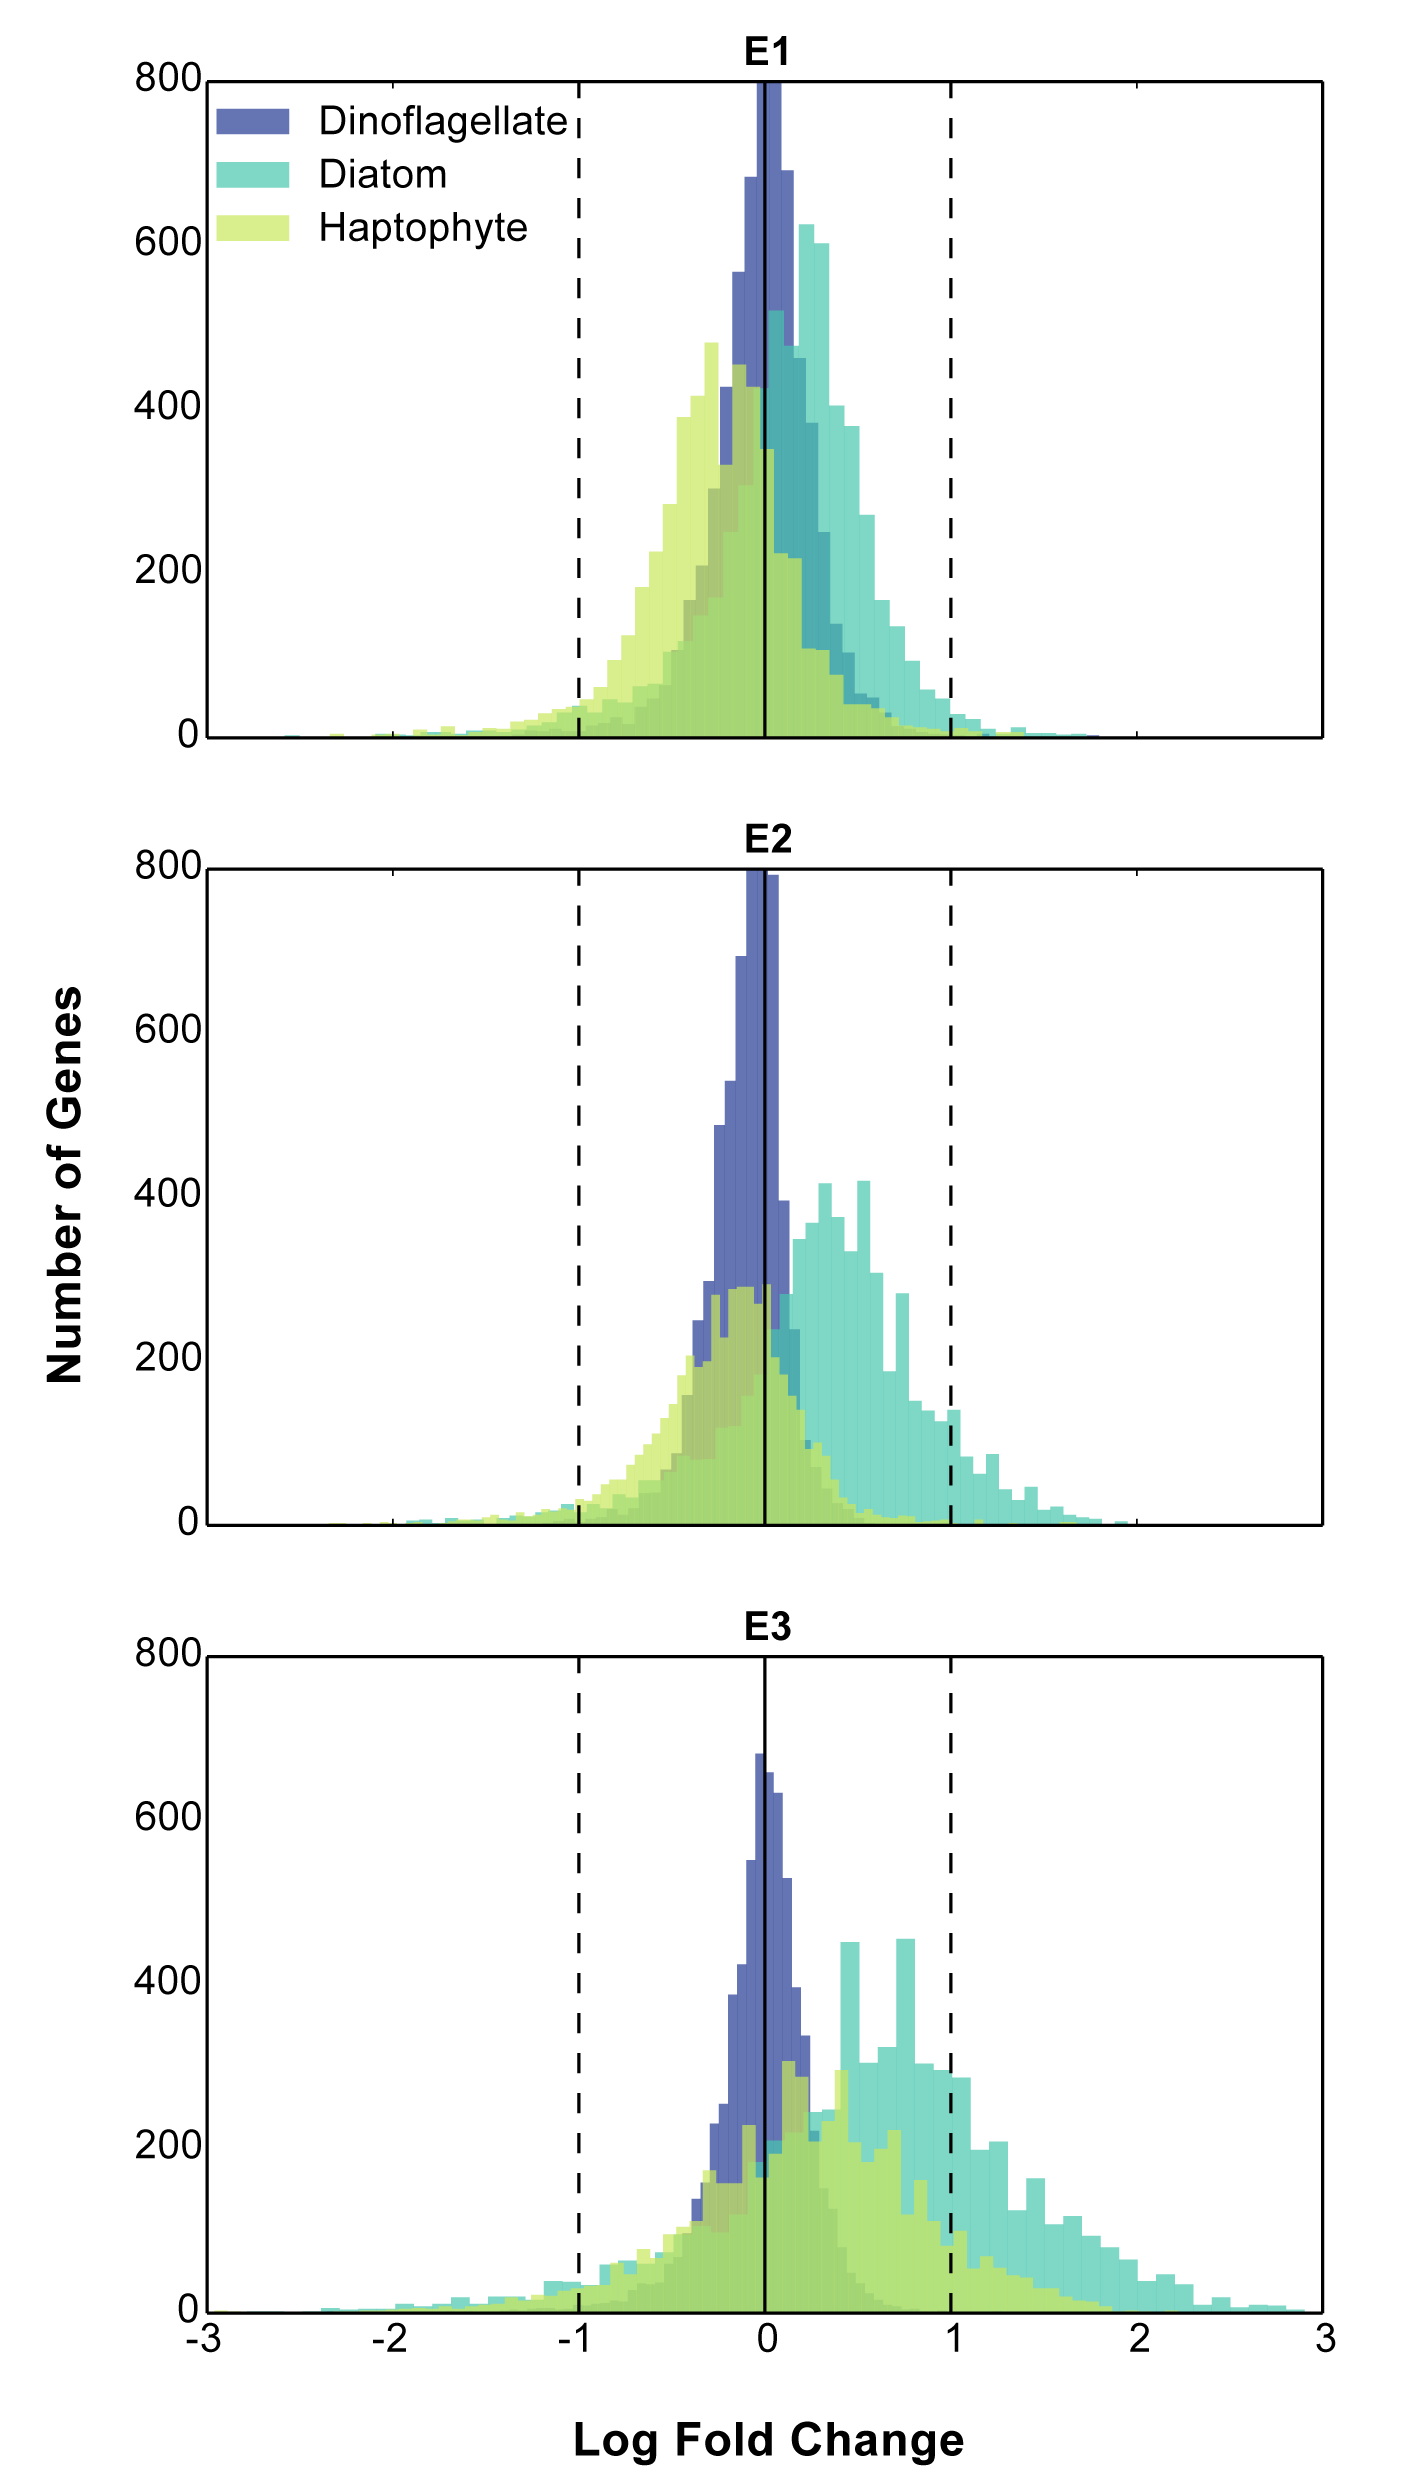
\includegraphics[width=.75\textwidth]{Images/C4_FigureS4.png}
    \caption[Distribution of log fold change following deep seawater (DSW) addition]{Distribution of log fold change following deep seawater (DSW) addition. Histogram of the number of genes falling within each of the log fold change bins for diatoms, haptophytes and dinoflagellates. Solid line indicates no fold change; dashed lines indicate 2 fold-change both up and down.}
  \label{fig:a4f4}
\end{figure}


%Supplemental Figure 5: Weight venn diagrams for up and down regulated genes

\begin{figure}[p!]
  \centering
    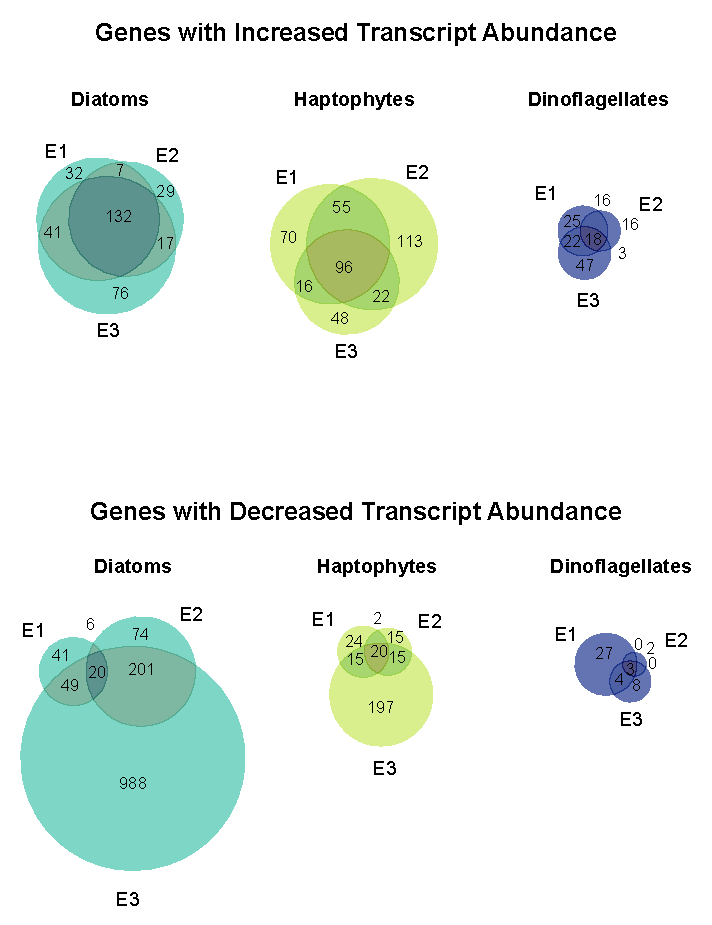
\includegraphics[width=1\textwidth]{Images/C4_FigureS5.pdf}
    \caption[Weighted Venn diagrams of genes with significantly different abundances following deep seawater (DSW) addition by functional group]{Weighted Venn diagrams of genes with significantly different abundances following deep seawater (DSW) addition by functional group. The uniqueness of KEGG orthologs with increased or decreased abundances as determined by ASC (2 fold-change, post-p > 0.95) across experiments was assessed for diatoms, haptophytes, and dinoflagellates.}
  \label{fig:a4f5}
\end{figure}


%Supplemental Figure 6: MANTA Plots

\begin{figure}[p!]
  \centering
    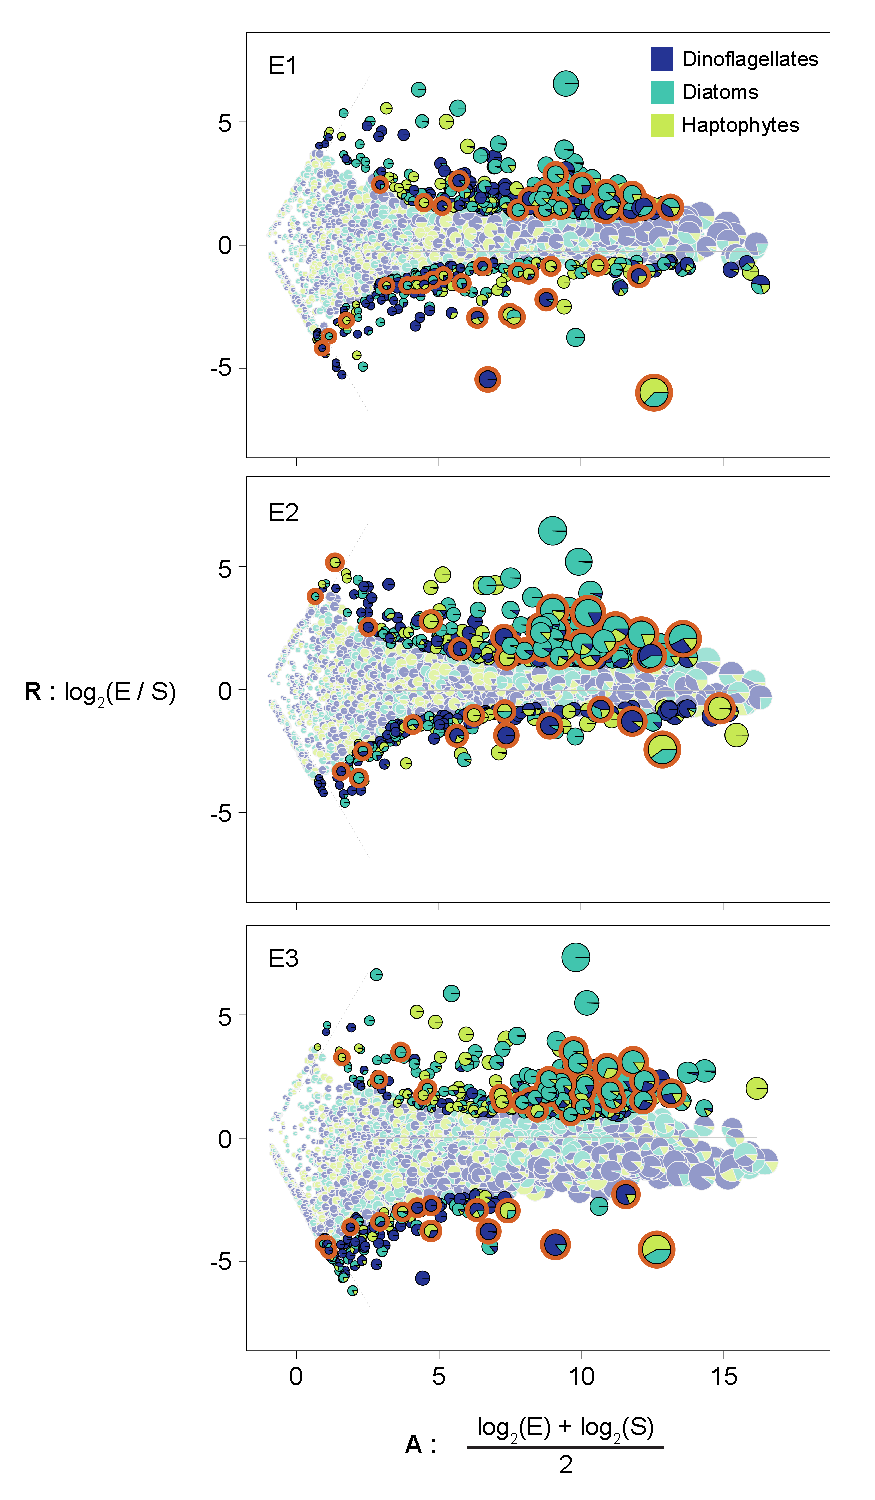
\includegraphics[width=.7\textwidth]{Images/C4_FigureS6.pdf}
    \caption[Microbial Assemblage Normalized Transcript Analysis (MANTA) ratio-averaged plots for global shifts in expression of KEGG orthologs]{Microbial Assemblage Normalized Transcript Analysis (MANTA) ratio-averaged plots for global shifts in expression of KEGG orthologs. Fold change ratio (R) and average read count (A) are plotted for read counts in the \emph{in situ} (S) and deep seawater (DSW) amendment (E) samples across the three sample pairs (S1:E1, S2:E2, S3:E3). The trimmed mean of fold-change values is noted as a gray solid line; orthologs unique to one library are separated by gray dashed lines. Pies indicate the taxonomic distribution of orthologous reads across the three functional groups. KEGG orthologs that were significantly differentially expressed (DE) (adjusted $P > 0.05$) are outlined in black and those not significantly DE are outlined in gray. DE KEGG orthologs that fall in the Energy Metabolism KEGG module are outlined in orange.}
  \label{fig:a4f6}
\end{figure}

%Supplemental Figure 7: QMF across incubation experiments

\begin{figure}[p!]
  \centering
    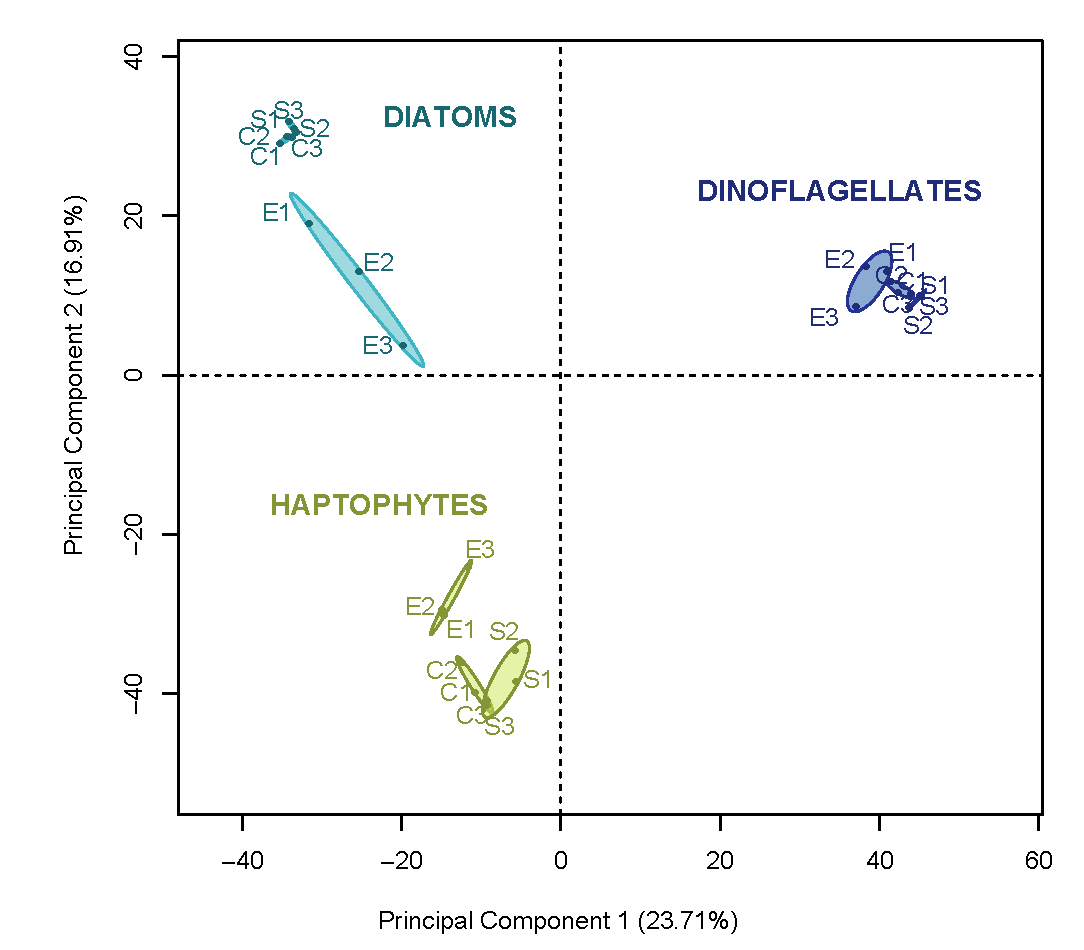
\includegraphics[width=1\textwidth]{Images/C4_FigureS7.pdf}
    \caption[Principal component analysis of the quantitative metabolic fingerprint (QMF) signals across \emph{in situ}, no addition control, and deep seawater amended samples]{Principal component analysis of the quantitative metabolic fingerprint (QMF) signals across \emph{in situ}, no addition control, and deep seawater (DSW) amended samples. Principal component analysis of the QMF signals for each of the functional groups across \emph{in situ} (S1-S3), control no addition (C1-C3) and DSW amendment (E1-E3); 95\% confidence ellipses are indicated for each of the sample types by functional group.}
  \label{fig:a4f7}
\end{figure}

\clearpage

\subsection{Supplemental Tables}

% Supplemental table with nutrient concentrations post treatment run for E and C
\begin{table}[h!]
\centering
\caption[Macronutrient concentrations in deep seawater ammendment and the incubation experiments after 168 hours]{Macronutrient concentrations in control no addition (C), DSW-amended incubations (E), and 700 m water used in DSW amendment incubations}
\label{tab:a4t1}
\newcolumntype{C}[1]{>{\centering\let\newline\\\arraybackslash\hspace{.5pt}}m{#1}}
\begin{tabular}{ccccc}

    
\hline
\multicolumn{1}{|c|}{\multirow{2}{*}{\textbf{Treatment}}} & \multicolumn{1}{c|}{\multirow{2}{*}{\textbf{\begin{tabular}[c]{@{}c@{}}Time post \\ inoculation (hours)\end{tabular}}}} & \multicolumn{1}{c|}{\multirow{2}{*}{\textbf{\begin{tabular}[c]{@{}c@{}}NO2 + NO3 \\ ($\mu M$)\end{tabular}}}} & \multicolumn{1}{c|}{\multirow{2}{*}{\textbf{\begin{tabular}[c]{@{}c@{}}PO4 \\ ($\mu M$)\end{tabular}}}} & \multicolumn{1}{c|}{\multirow{2}{*}{\textbf{\begin{tabular}[c]{@{}c@{}}Si\\ ($\mu M$)\end{tabular}}}} \\

\multicolumn{1}{|c|}{}                                    & \multicolumn{1}{c|}{}                                                        & \multicolumn{1}{c|}{}                                                                                    & \multicolumn{1}{c|}{}                                                                              & \multicolumn{1}{c|}{}                                                                            \\ \hline
\multicolumn{1}{|c|}{\textbf{C} (control no addition) *}  & \multicolumn{1}{c|}{168}                                                     & \multicolumn{1}{c|}{$0.12 \pm 0.03$}                                                                         & \multicolumn{1}{c|}{$0.12 \pm 0.02$}                                                                   & \multicolumn{1}{c|}{$1.91 \pm 0.2$}                                                                  \\ \hline
\multicolumn{1}{|c|}{\textbf{E} (+ 10\% DSW) *}           & \multicolumn{1}{c|}{168}                                                     & \multicolumn{1}{c|}{$1.9 \pm  .93$}                                                                          & \multicolumn{1}{c|}{$0.23 \pm 0.05$}                                                                   & \multicolumn{1}{c|}{$8.46 \pm 3.11$}                                                                 \\ \hline
\multicolumn{1}{|c|}{\textbf{DSW} (700 m water) *}        & \multicolumn{1}{c|}{N/A}                                                     & \multicolumn{1}{c|}{$37.5 \pm 1.68$}                                                                         & \multicolumn{1}{c|}{$3.14 \pm 0.03$}                                                                   & \multicolumn{1}{c|}{$83.4 \pm 9.33$}                                                                 \\ \hline
\multicolumn{5}{l}{\textit{* Nutrient data averaged for E1 and E2, nutrients were not assayed on E3.}}                                                                                                                                                                                                                                                                                                                                                     
\end{tabular}
\end{table}


%%%%%%%%%%%%%%%%%%%%%%%%%%%%

%%%%%%%%%%%%%%%%%%%%%%%%%%%_________________CHAPTERTHREE_________________%%%%%%%%%%%%%%%%%%%%%%%%%%%

%%%%%%%%%%%%%%%%%%%%%%%%%%%

\chapter{Chapter 3 Supplemental Information}
\label{sec:app3}
\clearpage
\section{Supplemental Figures}

%Supplemental Figure 1: Cell counts in NB 
\begin{figure}[h!]
  \centering
    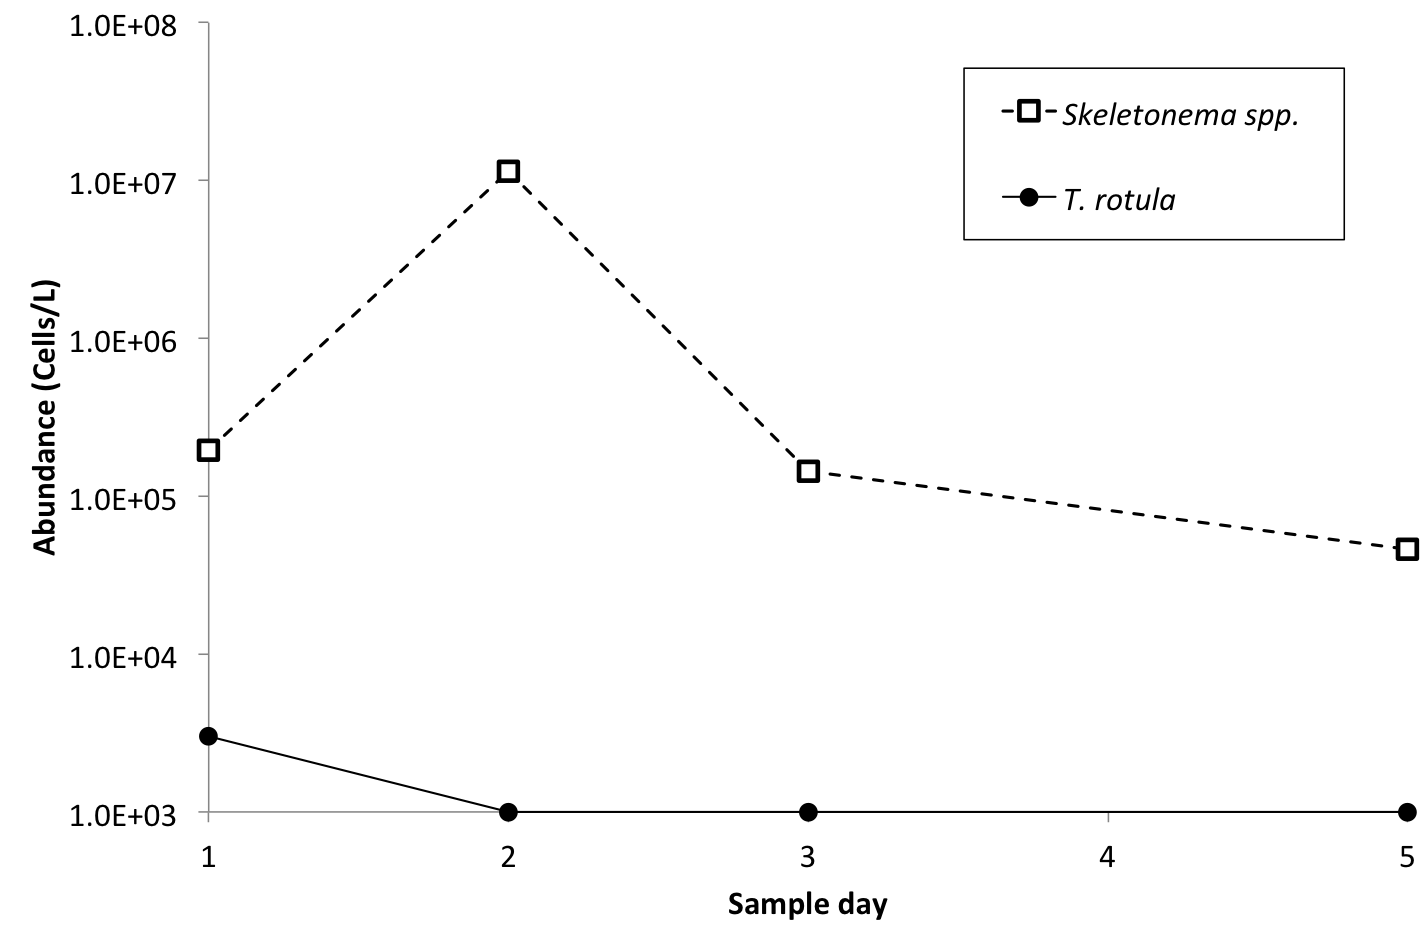
\includegraphics[width=1\textwidth]{Images/C3_SFigure1_CellCounts.png}
    \caption[Cell counts in Narragansett Bay during the spring of 2012]{Abundance estimation from cell counts of \textit{Skeletonema} spp. and \textit{T. rotula} across the five sample points during the spring of 2012. }
  \label{fig:a3f1}
\end{figure}


%Supplemental Figure 2: KEGG linear correlation
\begin{figure}[p!]
  \centering
    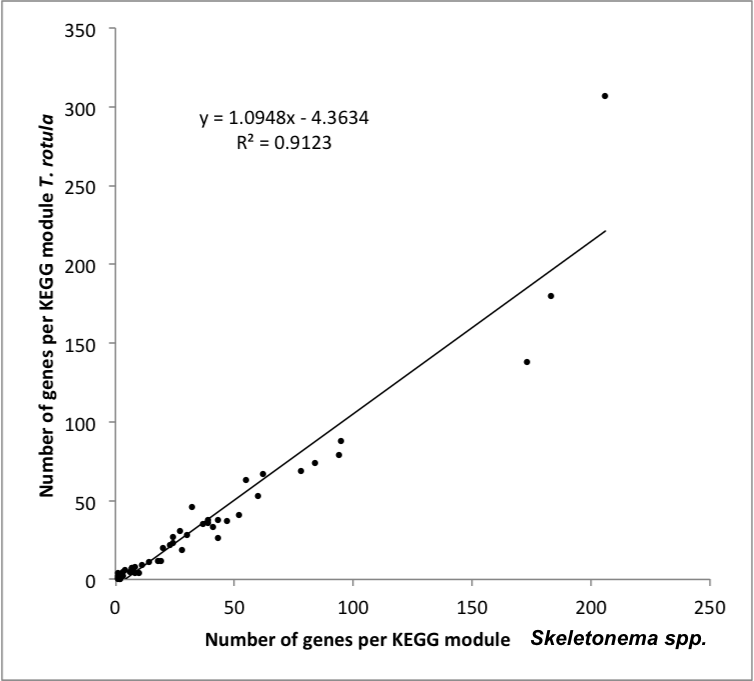
\includegraphics[width=1\textwidth]{Images/C3_SFigure2_KEGGModuleGeneContent2.png}
    \caption[Comparison of KEGG module content between \textit{Skeletonema} spp. and \textit{T. rotula} ]{Total number of genes assigned to each KEGG module for \textit{Skeletonema} spp. and \textit{T. rotula}.}
  \label{fig:a3f2}
\end{figure}


%Supplemental Figure 3: Hierarchical clustering of S and T across time
\begin{figure}[p!]
  \centering
    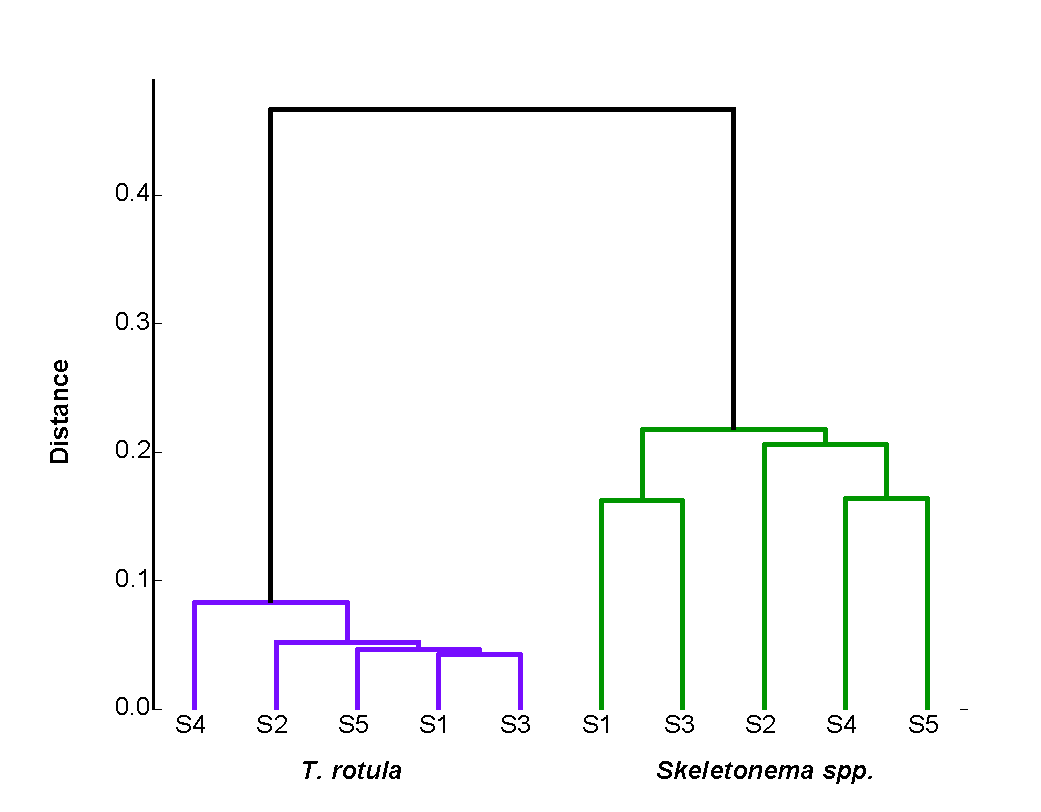
\includegraphics[width=1\textwidth]{Images/C3_SFigure3_Dendrogram.pdf}
    \caption[Hierarchical clustering of QMF signatures across species and samples]{Dendrogram depicting hierarchical clustering of samples based on relative expression of KEGG modules (Figure 2) across the five samples S1-S5 for \textit{Skeletonema} spp. and \textit{T. rotula}.}
  \label{fig:a3f3}
\end{figure}

%Supplemental Figure 4: Stable gene expression across time
\begin{figure}[p!]
  \centering
    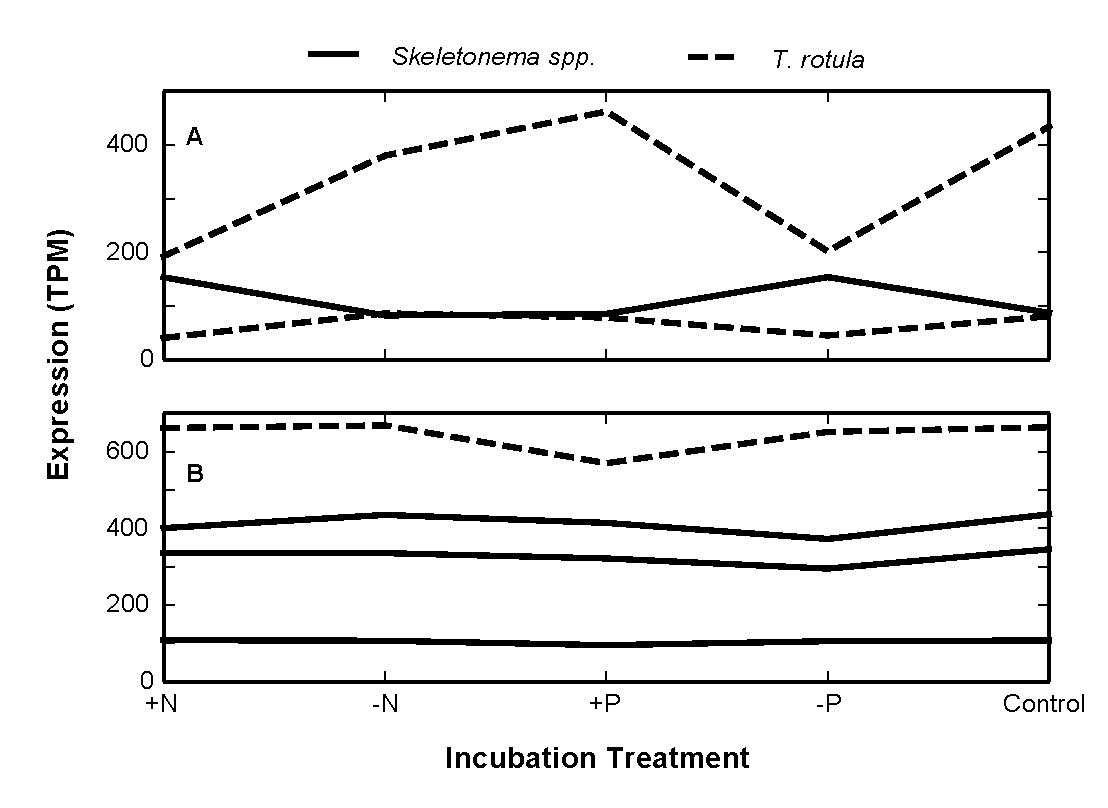
\includegraphics[width=1\textwidth]{Images/C3_SFigure4_StableGenePlot_wActin.pdf}
    \caption[Expression of stable reference genes in the field]{Expression of stable reference genes identified based on literature and statistical parsing in nutrient amendment incubation. (A) The expression in tags per million ($TPM$) of stable reference genes identified in \textit{T. rotula} (dashed line) and \textit{Skeletonema} spp.  (solid lines) based on homology (e-value < 1e-5) to a known reference genes in \textit{T. pseudonana}, ACT1 (Thaps\_25772), in nutrient incubations. (B) Also shown are reference genes identified in the incubation experiments, using statistical analysis of sequence counts \citep{Alexander2012, Wu2010}, and nutrient incubations }
  \label{fig:a3f4}
\end{figure}

%Supplemental Figure 5: RR gene composition
\begin{figure}[p!]
  \centering
    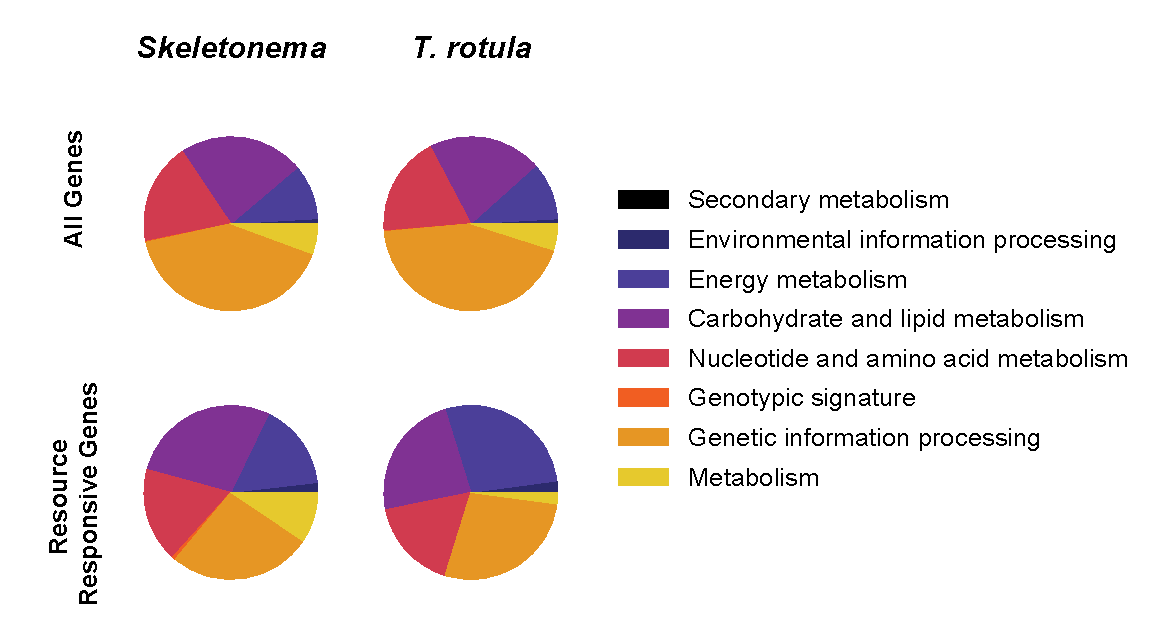
\includegraphics[width=1\textwidth]{Images/C3_SFigure5_RR_All_Genes_Pie.pdf}
    \caption[Functional compoosition of the reference transcriptome and resource-responsive gene sets]{Functional composition of the reference transcriptome and resource-responsive (RR) gene subset for \textit{T. rotula} and \textit{Skeletonema} spp. (A) RR gene sets were identified through cross comparison of like-nutrient incubations (i.e. +N vs. -N and +P vs. -P), using ASC (fold change = 2, post-$p > 0.95$). The relative functional categorization of the reference transcriptomes and RR gene set for \textit{T. rotula} and \textit{Skeletonema} spp. based on KEGG ontology as assigned by KAAS is depicted at the module-level.}
  \label{fig:a3f5}
\end{figure}

%Supplemental Figure 6: Expression of nitrate reductase

\begin{figure}[p!]
  \centering
    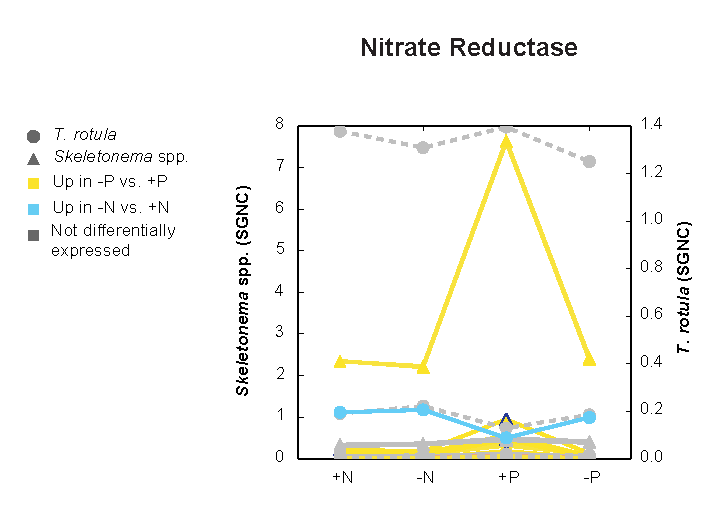
\includegraphics[width=1\textwidth]{Images/C3_SFigure6_SGNC_NitrateReductase.pdf}
    \caption[Relative expression of nitrate reducatses across incubation experiments]{The relative expression in stable gene normalized counts ($SGNC$) of the assimilatory nitrate reductase gene cluster across the incubation experiment treatments. Significance of regulation between the treatments is denoted by the color of the line; organisms are denoted by the shapes of the marker.}
  \label{fig:a3f6}
\end{figure}

%Supplemental Figure 7: Cluster Analysis


\begin{figure}[p!]
  \centering
    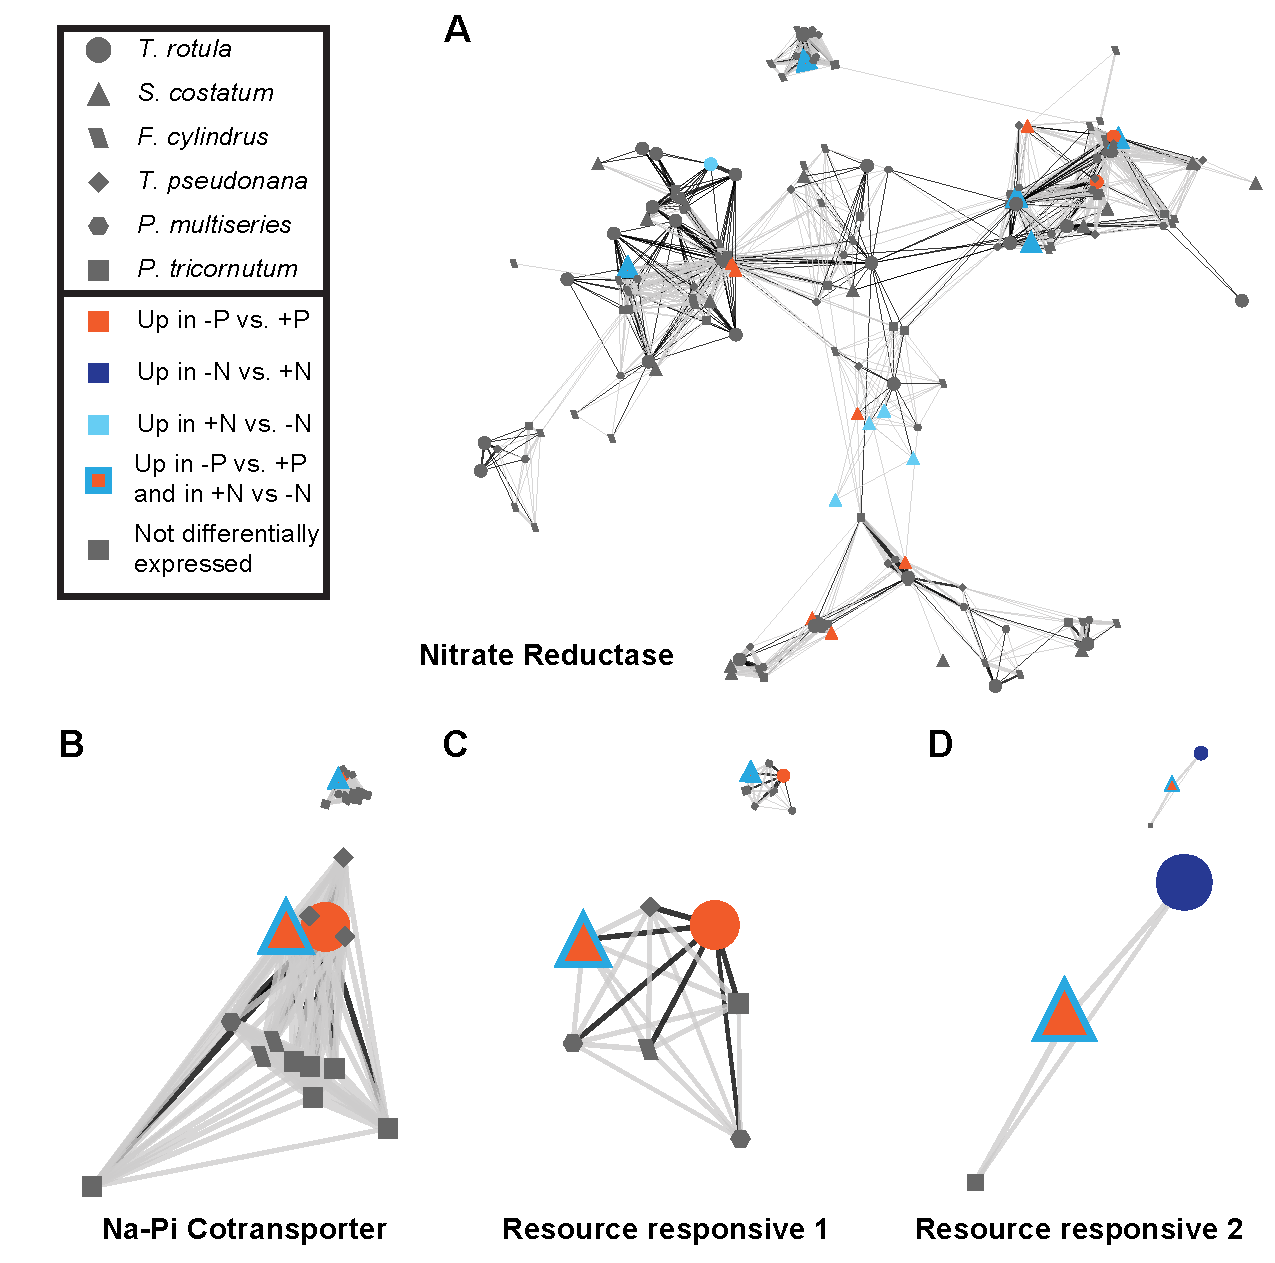
\includegraphics[width=1\textwidth]{Images/C3_SFigure7_ClusterAnalysis_v5.pdf}
    \caption[Gene cluster analysis of nutrient-responsive genes]{Gene cluster known nutrient-responsive genes in \textit{T. pseudonana}: (A) assimilatory nitrate reductase and (B) sodium-phosphate cotransporter and novel resource-responsive (RR) gene families: (C) RR1 and (D) RR2. Transcripts from the transcriptomes of \textit{T. rotula} and \textit{Skeletonema} spp. were clustered based upon relative homology with available diatom genomes: \textit{F. cylindrus}, \textit{P. tricornitum}, \textit{P. multiseries}, and \textit{T. pseudonana}. Symbols indicate different species, while color indicates regulation in the field incubation experiments. Two nodes within a gene cluster are connected by an edge if they share a homologous protein (reciprocal BLAST hit with a minimum of 1e-5 score and minimum 20\% identity). Gene clusters are visualized using an edge-weighted spring-embedded model based on e-value, meaning that genes that are closer together are more similar. The width of the line correlates to the magnitude of the e-value, with lower e-values represented by thicker lines and higher e-values represented by thinner lines.}
  \label{fig:a3f7}
\end{figure}

%Supplemental Figure 8: Conceptual schematic of STD niche space

\begin{figure}[p!]
  \centering
    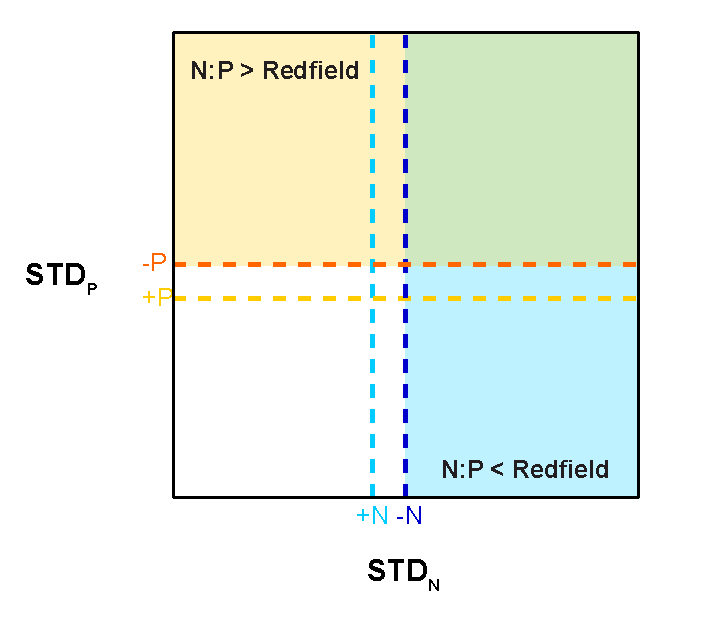
\includegraphics[width=1\textwidth]{Images/C3_SFigure8_Schematic_Quadrants.pdf}
    \caption[Conceptual schemiatic of $STD_N$ plotted against $STD_P$]{A conceptual schematic of $STD_N$ plotted against $STD_P$ hypothesized regions of N:P > Redfield physiology and N:P < Redfield physiology highlighted.}
  \label{fig:a3f8}
\end{figure}


%Supplemental Figure 9: NISP Dn genes
\begin{landscape}
   \centering
   \null         %%<---- this is needed
   \vfill        %%<-----here

	\begin{figure}
  	\centering
    	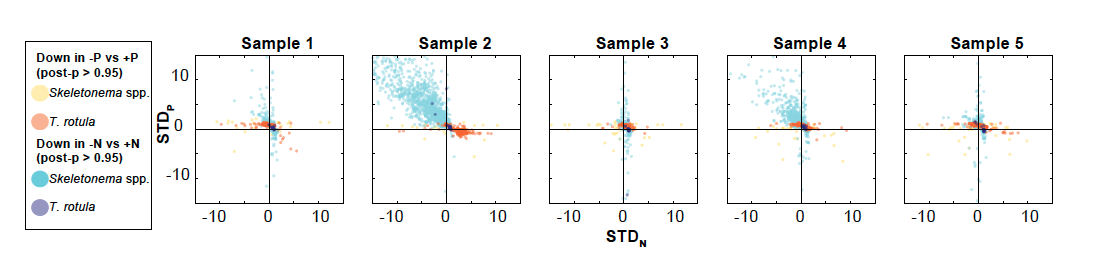
\includegraphics[width=1.3\textwidth]{Images/C3_SFigure9_NISP_DNGenes.png}
    	\caption[Evolution of niche space indexing over for significantly down-regualted genes]{Evolution of niche space indexing over time in Narragansett Bay for \textit{T. rotula} and \textit{Skeletonema} spp.. The stable gene normalized field signal from genes identified as significantly (2-fold change, post$-p > 0.95$) down-regulated in -P vs +P for Skeletonema spp. (yellow) and \textit{T. rotula} (orange) and in -N vs +N for for \textit{Skeletonema} spp. (cyan) and \textit{T. rotula} (dark blue) was proportionalized relative to the expression for those genes in nutrient incubations, yielding the $STD_N$ and $STD_P$. These data are plotted for Sample 1 through Sample 5.}
  	\label{fig:a3f9}
	\end{figure}
    \vfill        %%<----- and here
\end{landscape}

%Supplemental Figure 10: Percentage of RR genes by quadrant

\begin{figure}[h!]
  \centering
    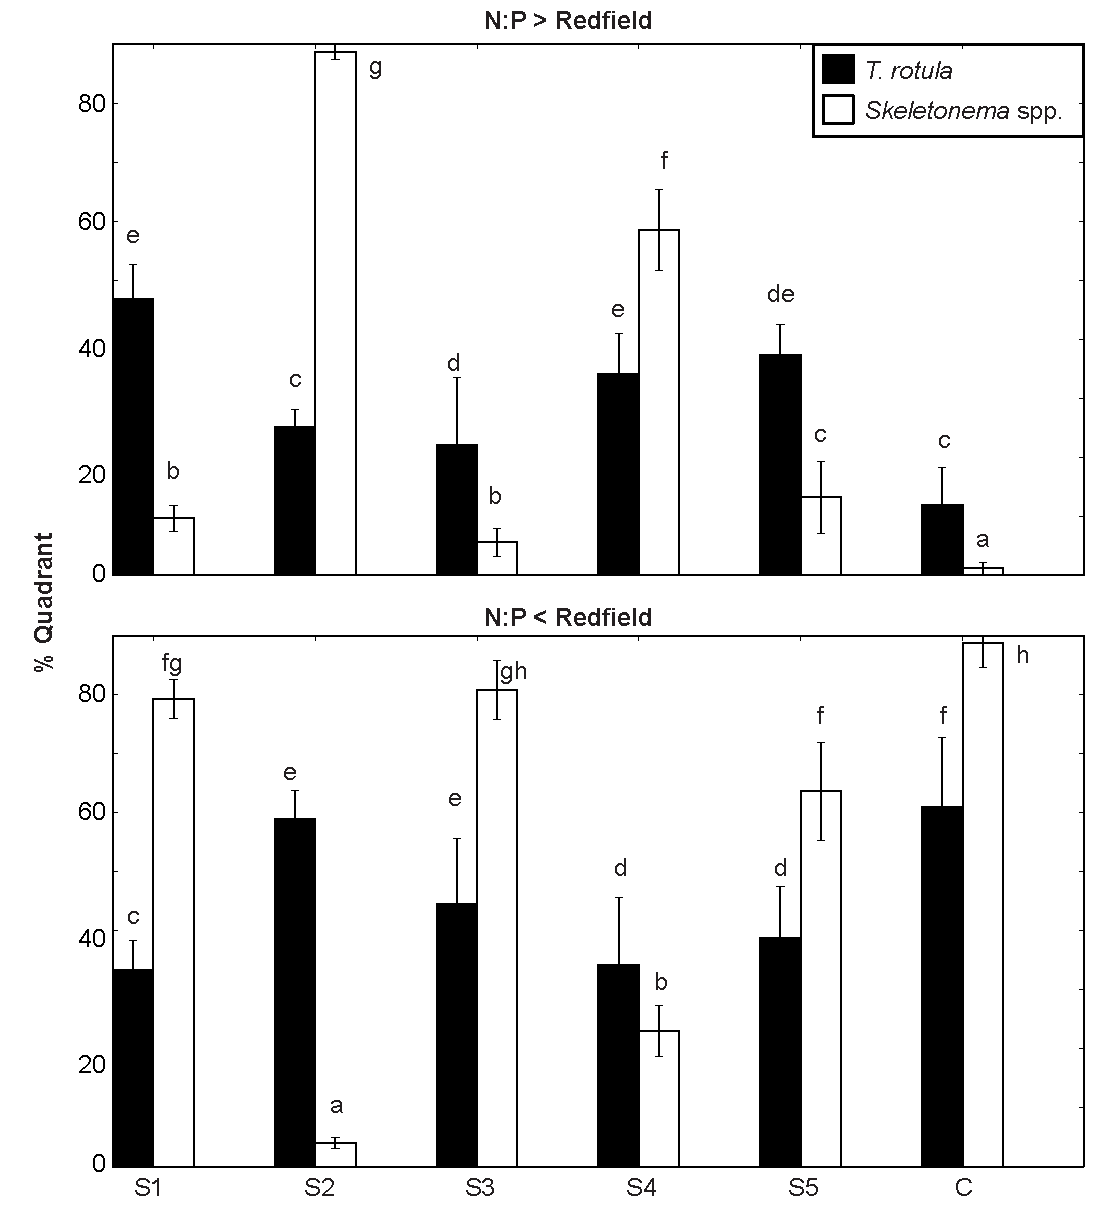
\includegraphics[width=1\textwidth]{Images/C3_SFigure10_BarGraph_Quadrant_2575_stats.pdf}
    \caption[The percentage of identified nutrient responsive genes falling into the N:P > Redfield and N:P < Redfield quadrants with varried cutoffs]{The percentage of identified nutrient responsive genes falling into the N:P > Redfield and N:P < Redfield quadrants for \textit{T. rotula} and \textit{Skeletonema} spp.. The total number of genes falling into the N:P > Redfield quadrant ($STD_P > C$; $STD_N < C$, for $0.25 < C < 0.75$) and the N:P < Redfield quadrant ($STD_P$ < C; $STD_N > C$, for $0.25 < C < 0.75$). The value of C was varied over 10 different values and the average percentages of genes falling into each of the quadrants is depicted above based on the size of the circle at the median $STD_N$ and $STD_P$ for the genes in the quadrant. Similarity of data between species by quadrant was assessed using an analysis of variance (ANOVA) with a generalized linear model. The results from a post hoc Tukey test show the divergence of species across time ($p < 0.05$).}
  \label{fig:a3f10}
\end{figure}

%Supplemental Figure 11: Quadrant localization with varying stable reference genes

\begin{figure}[p!]
  \centering
    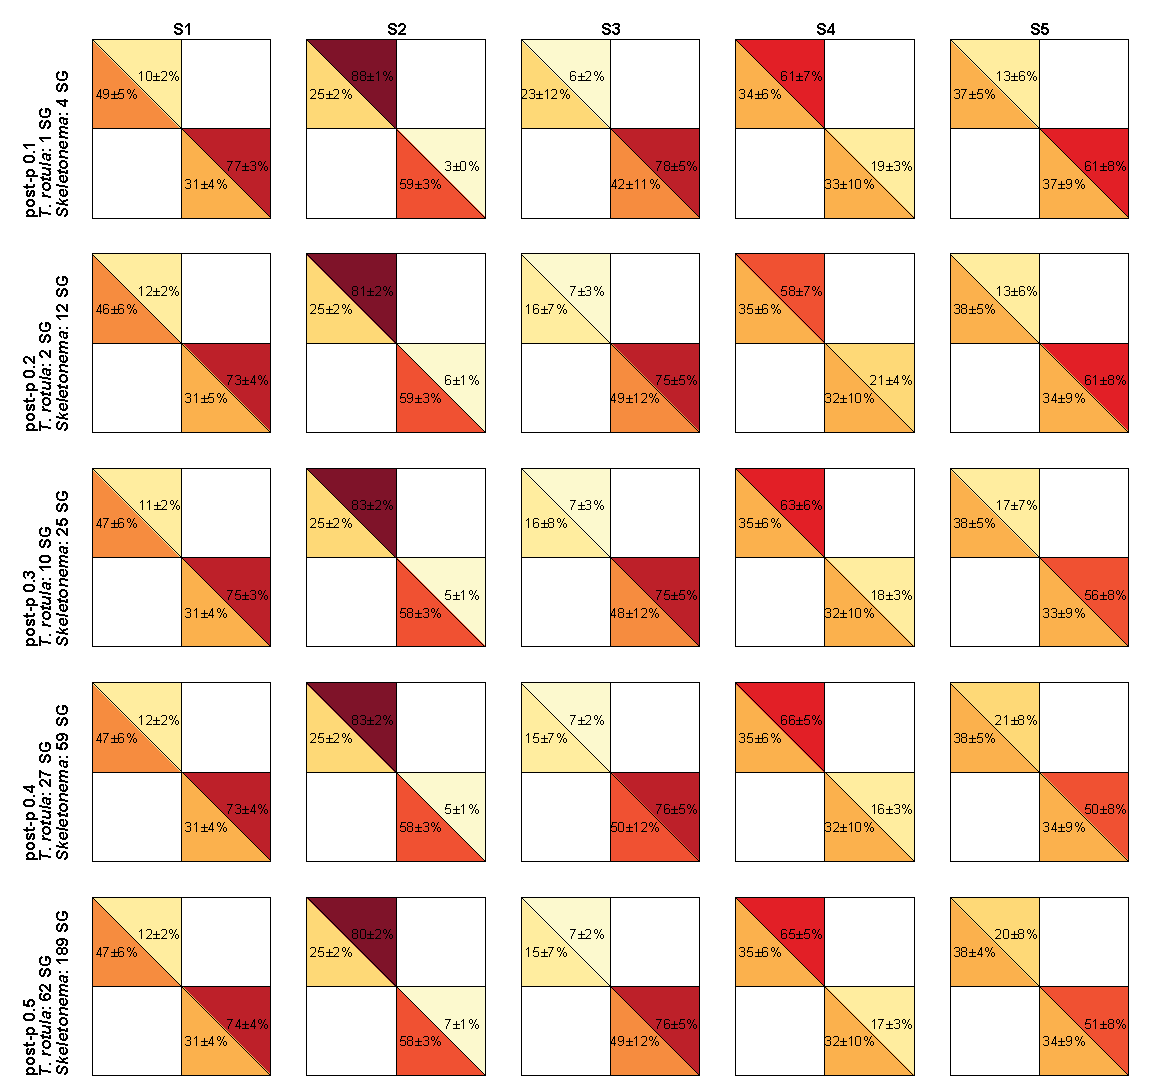
\includegraphics[width=1\textwidth]{Images/C3_SFigure11_Quadrant.pdf}
    \caption[The impact of stable gene selction of quadrant localization]{The impact of stable gene selection on the quadrant localization of the resource responsive gene sets. The posterior probability cutoff used in the selection of stable genes was varied from 0.1 to 0.5 for a fold change of 1.25. The percentage of identified nutrient responsive genes falling into the N:P > Redfield and N:P < Redfield quadrants for \textit{T. rotula} and \textit{Skeletonema} spp. across the five sample points and five posterior probability values is depicted.}
  \label{fig:a3f11}
\end{figure}



\section{Supplemental Tables}

%Supplemental Table 1: library stats

\begin{table}[h!]
\centering
\caption[The total number of paired end reads after quality control and trimming and the percentage of reads mapping]{The total number of paired end reads after quality control and trimming and the percentage of reads mapping to the \textit{T. pseudonana} genome, \textit{T. rotula} transcriptome, and \textit{S. costatum} transcriptome.}
\label{tab:a3t1}
\newcolumntype{L}[1]{>{\raggedright\let\newline\\\arraybackslash\hspace{0pt}}m{#1}}
\label{my-label}
\begin{tabular}{lp{2cm}lll}
\multirow{2}{*}{Sample} & \multirow{2}{*}{\parbox{2cm}{Library Size (PE reads)}} & \multicolumn{3}{c}{\textbf{Representation in library}}             \\ 
                        &                                          & \textit{T. pseudonana} & \textit{T. rotula} & \textit{S. costatum} \\ \Xhline{2\arrayrulewidth}
S1                      & 89455034                                 & 2.98\%                 & 17.50\%            & 33.50\%              \\ \hline
S2                      & 64888267                                 & 0.41\%                 & 11.70\%            & 54.90\%              \\ \hline
S3                      & 103250243                                & 0.39\%                 & 7.30\%             & 9.00\%               \\ \hline
S4                      & 45370867                                 & 0.68\%                 & 8.80\%             & 8.30\%               \\ \hline
S5                      & 55061692                                 & 0.88\%                 & 10.40\%            & 11.20\%              \\ \hline
Ambient Control         & 51508197                                 & 0.27\%                 & 13.40\%            & 8.00\%               \\ \hline
+N                      & 58626239                                 & 0.43\%                 & 6.10\%             & 5.30\%               \\ \hline
-N                      & 44561851                                 & 0.41\%                 & 8.70\%             & 8.30\%               \\ \hline
+P                      & 51130364                                 & 0.29\%                 & 8.50\%             & 8.00\%               \\ \hline
-P                      & 58834022                                 & 0.40\%                 & 6.60\%             & 6.50\%               \\ \hline
\end{tabular}
\end{table}

%Supplememntal Table 2: nutrient concentrations used in incubations

\begin{table}[h!]
\centering
\caption[Nutrient concentrations used in nutrient amendment incubations. ]{Nutrient concentrations used in nutrient amendment incubations.}
\label{tab:a3t2}
\begin{tabular}{llllll}
            & \multicolumn{5}{c}{Treatment}                                        \\
Amendment   & Ambient Control & +N         & +P        & -N          & -P          \\\Xhline{2\arrayrulewidth}
Nitrate     & -               & $10 \mu M$ & -         & -           & $10 \mu M$  \\
Phosphate   & -               & -          & $3 \mu M$ & $3 \mu M$   & -           \\
Silica      & -               & -          & -         & $68 \mu M$  & $68 \mu M$  \\
Iron        & -               & -          & -         & $4.6 \mu M$ & $4.6 \mu M$ \\
Vitamin B12 & -               & -          & -         & f/5         & f/5        
\end{tabular}
\end{table}

%Supplememntal Table 3: nutrient concentrations used in incubations

\begin{table}[h!]
\centering
\caption[Mapping statistics for \textit{T. rotula} and \textit{S. costatum} transcriptomes]{Total number of contigs in the \textit{T. rotula} and \textit{S. costatum} transcriptomes and the number of genes in each of the differentially regulated and stable groupings.}
\label{tab:a3t3}
\newcolumntype{L}[1]{>{\raggedright\let\newline\\\arraybackslash\hspace{0pt}}m{#1}}
\begin{tabular}{L{3.5cm}ll}
\hline
                                                                       & \textit{\textbf{T. rotula}} & \textit{\textbf{S. costatum}} \\ \Xhline{2\arrayrulewidth}

Number of contigs in transcriptome                                     & 22362                       & 27665                         \\ \hline
Pass 2 TPM cutoff                                                      & 4318                        & 20921                         \\ \hline
Up in -P vs +P                                                         & 249                         & 4754                          \\ \hline
Down in -P vs +P                                                       & 335                         & 52                            \\ \hline
Up in -N vs +N                                                         & 196                         & 9                             \\ \hline
Down in -N vs +N                                                       & 49                          & 1631                          \\ \hline
All differentially regulated (2 fold change, post-$p > 0.95$) & 775                         & 5136                          \\ \hline
Stable genes (1.25 fold change, post-$p < 0.1$)                  & 1                           & 4                             \\ \hline
\end{tabular}
\end{table}

\clearpage

\section{Supplemental Data}

    \begin{DS3}
    
    \item \label{DS31}: Annotations based on KEGG Ontology for \textit{Skeletonema} spp. and \textit{T. rotula} transcriptomes. \href{http://www.pnas.org/content/suppl/2015/04/09/1421993112.DCSupplemental/pnas.1421993112.sd01.xlsx}{Data Sheet 3-1} can be downloaded from the online version of the manuscript of \citet{Alexander2015} through \href{http://www.pnas.org/content/112/17/E2182.full}{\textit{Proceedings of the National Academy of Sciences}}. 
    \item \label{DS32}: Relative expression in tags per million (TPM) for genes identified as differentially or stably expressed in nutrient incubations. \href{http://www.pnas.org/content/suppl/2015/04/09/1421993112.DCSupplemental/pnas.1421993112.sd02.xlsx}{Data Sheet 3-2} can be downloaded from the online version of the manuscript of \citet{Alexander2015} through \href{http://www.pnas.org/content/112/17/E2182.full}{\textit{Proceedings of the National Academy of Sciences}}. 
  
    \end{DS3}



%%%%%%%%%%%%%%%%%%%%%%%%%%%%

%%%%%%%%%%%%%%%%%%%%%%%%%%%_________________CHAPTERFOUR_________________%%%%%%%%%%%%%%%%%%%%%%%%%%%

%%%%%%%%%%%%%%%%%%%%%%%%%%%

\chapter{Chapter 4 Supplemental Information}
\label{sec:app4}
\clearpage
\section{Supplemental Figures}

%Supplemental Figure 1: Chlorophyll values in experiments and in situ samples 
\begin{figure}[h!]
  \centering
    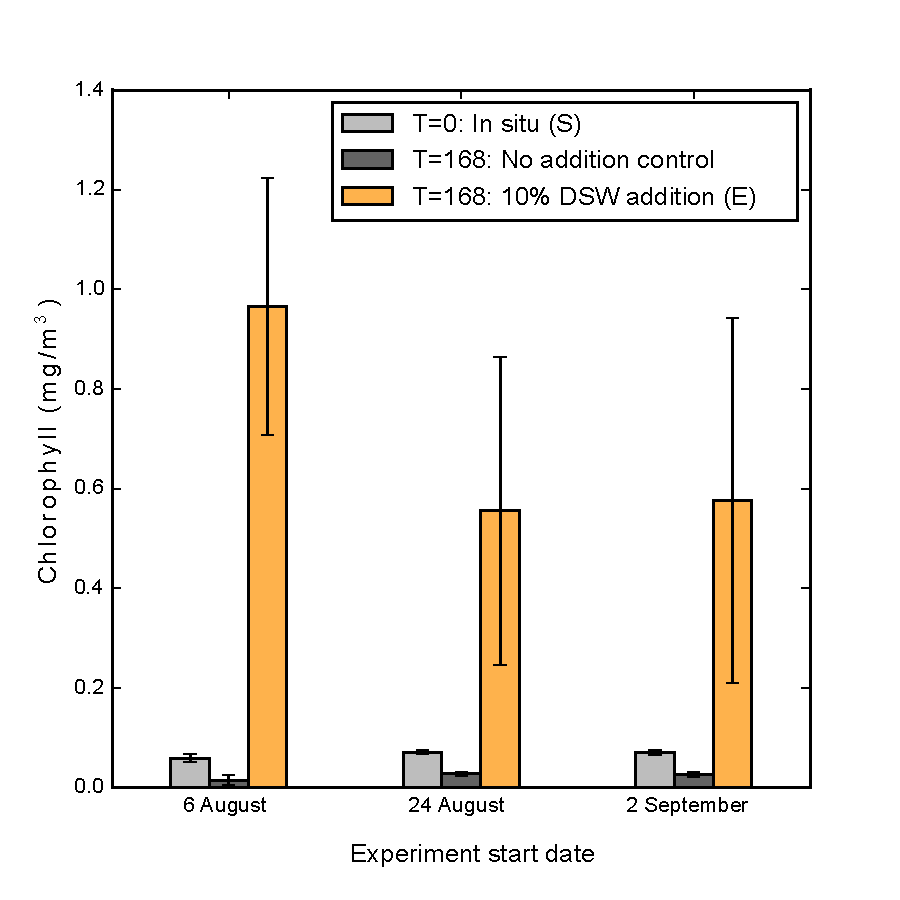
\includegraphics[width=1\textwidth]{Images/C4_FigureS1.pdf}
    \caption[Chlorophyll a of replicated experiments for \emph{in situ} samples, no addition control, and a 10\% deep seawater amendment]{Chlorophyll a of replicated experiments for \emph{in situ} samples (S), a no addition control, and a 10\% deep seawater (DSW) amendment (E). Incubation samples were harvested after 168 hours.}
  \label{fig:a4f1}
\end{figure}


%Supplemental Figure 2: Rank abundance shifts in species composition of diatoms, haptophytes and dinoflagellates

\begin{landscape}
 %  \null         %%<---- this is needed
   \vfill        %%<-----here
\begin{figure}[p!]
  \centering
    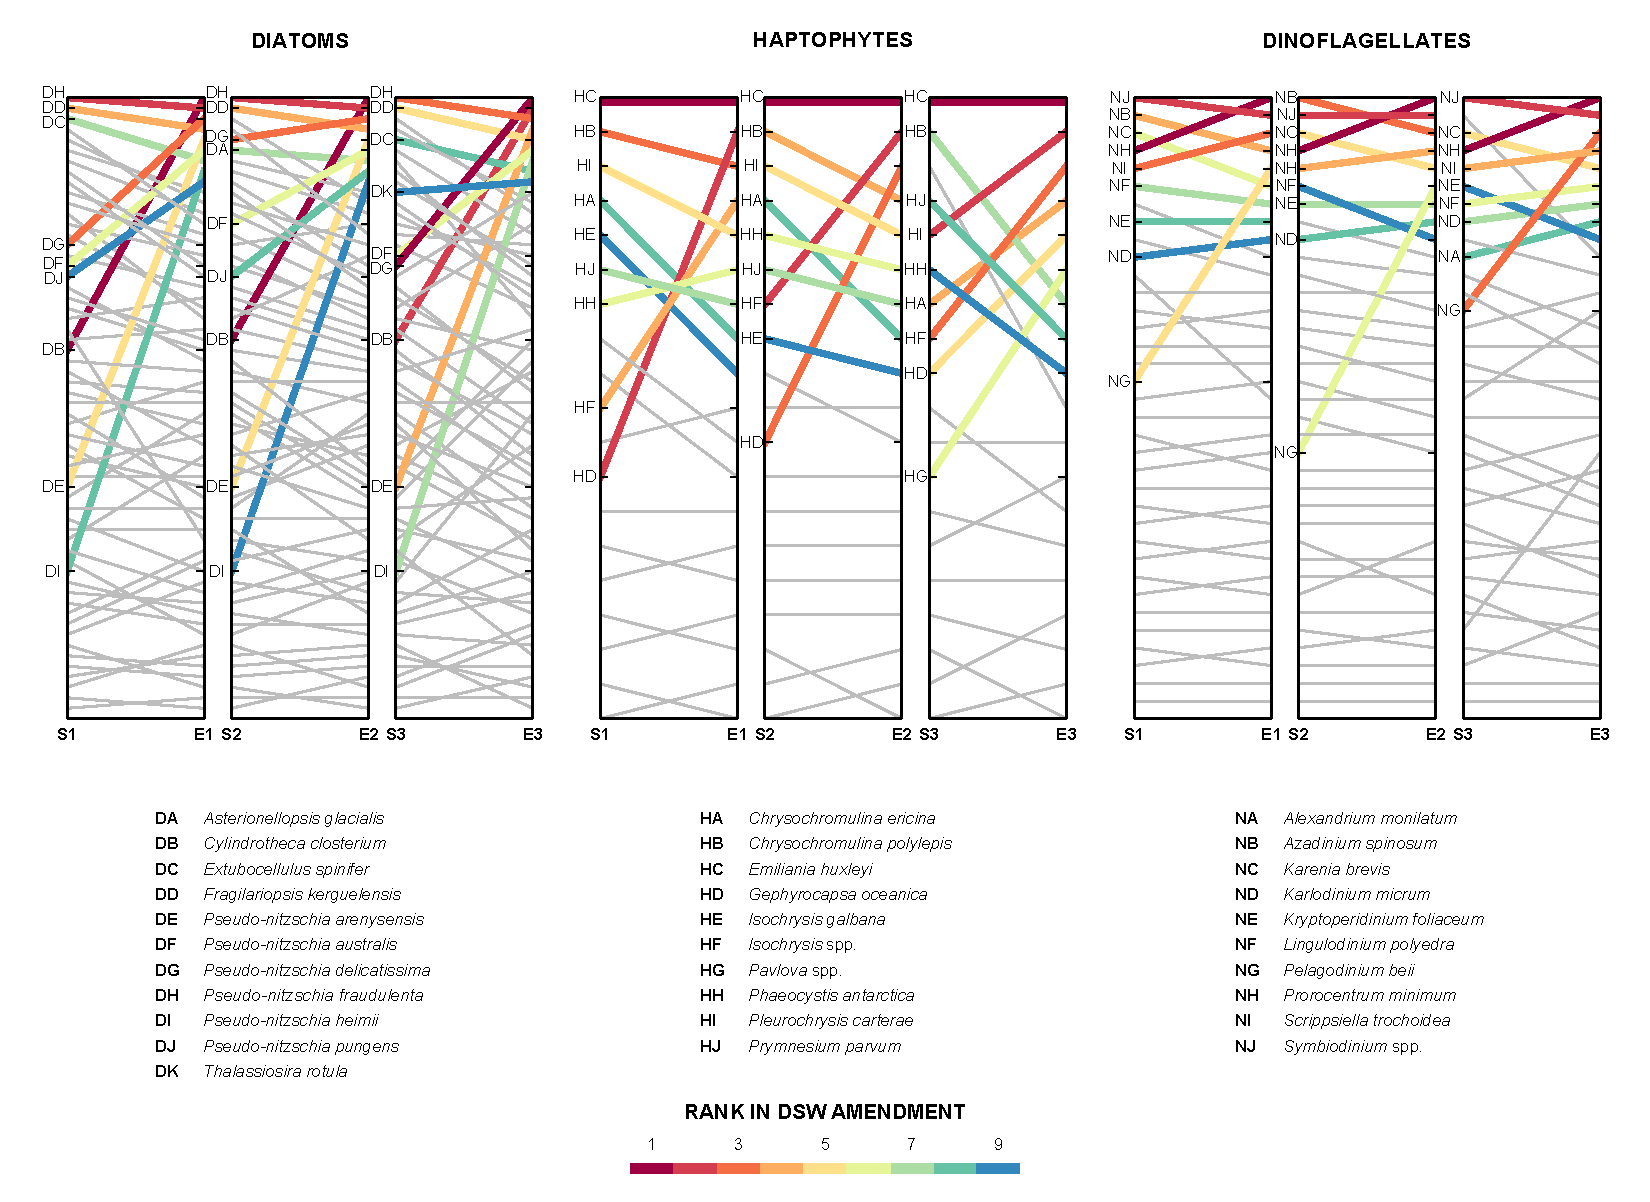
\includegraphics[width=1\textwidth]{Images/C4_FigureS2.pdf}
    \caption[Rank abundance shifts in the species composition of diatoms, haptophytes and dinoflagellates]{Rank abundance shifts in the species composition of diatoms, haptophytes and dinoflagellates for the three experiments. The relative shift in rank abundance for each species is depicted for each incubation experiment (E1-E3) following deep seawater (DSW) addition. The nine most abundant taxa following DSW addition are highlighted for each of the functional groups. Although the species that recruited the reads are denoted here this is highly driven by the composition of the database and does not necessarily indicate the actual species present, but rather the closest species present in the database.}
  \label{fig:a4f2}
\end{figure}
    \vfill        %%<----- and here
\end{landscape}


%Supplemental Figure 3: QMF Comparison across species


\begin{figure}[p!]
  \centering
    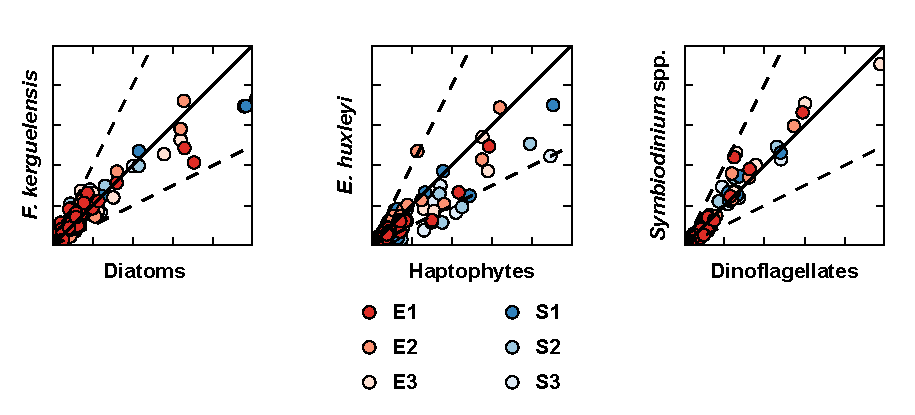
\includegraphics[width=1\textwidth]{Images/C4_FigureS3.pdf}
    \caption[Comparison of the quantitative metabolic fingerprint (QMF) between the whole functional group and representative taxa]{Comparison of the quantitative metabolic fingerprint (QMF) between the whole functional group and representative taxa. The proportion of reads falling into each of the modules depicted in Figure 2 is plotted for S1-S3 and E1-E3, comparing the summed functional group signal and that of a representative taxon. Color of the marker indicates the sample; solid and dashed lines mark the 1:1 and 1:2 lines, respectively.}
  \label{fig:a4f3}
\end{figure}

%Supplemental Figure 4: Distribution histogram

\begin{figure}[p!]
  \centering
    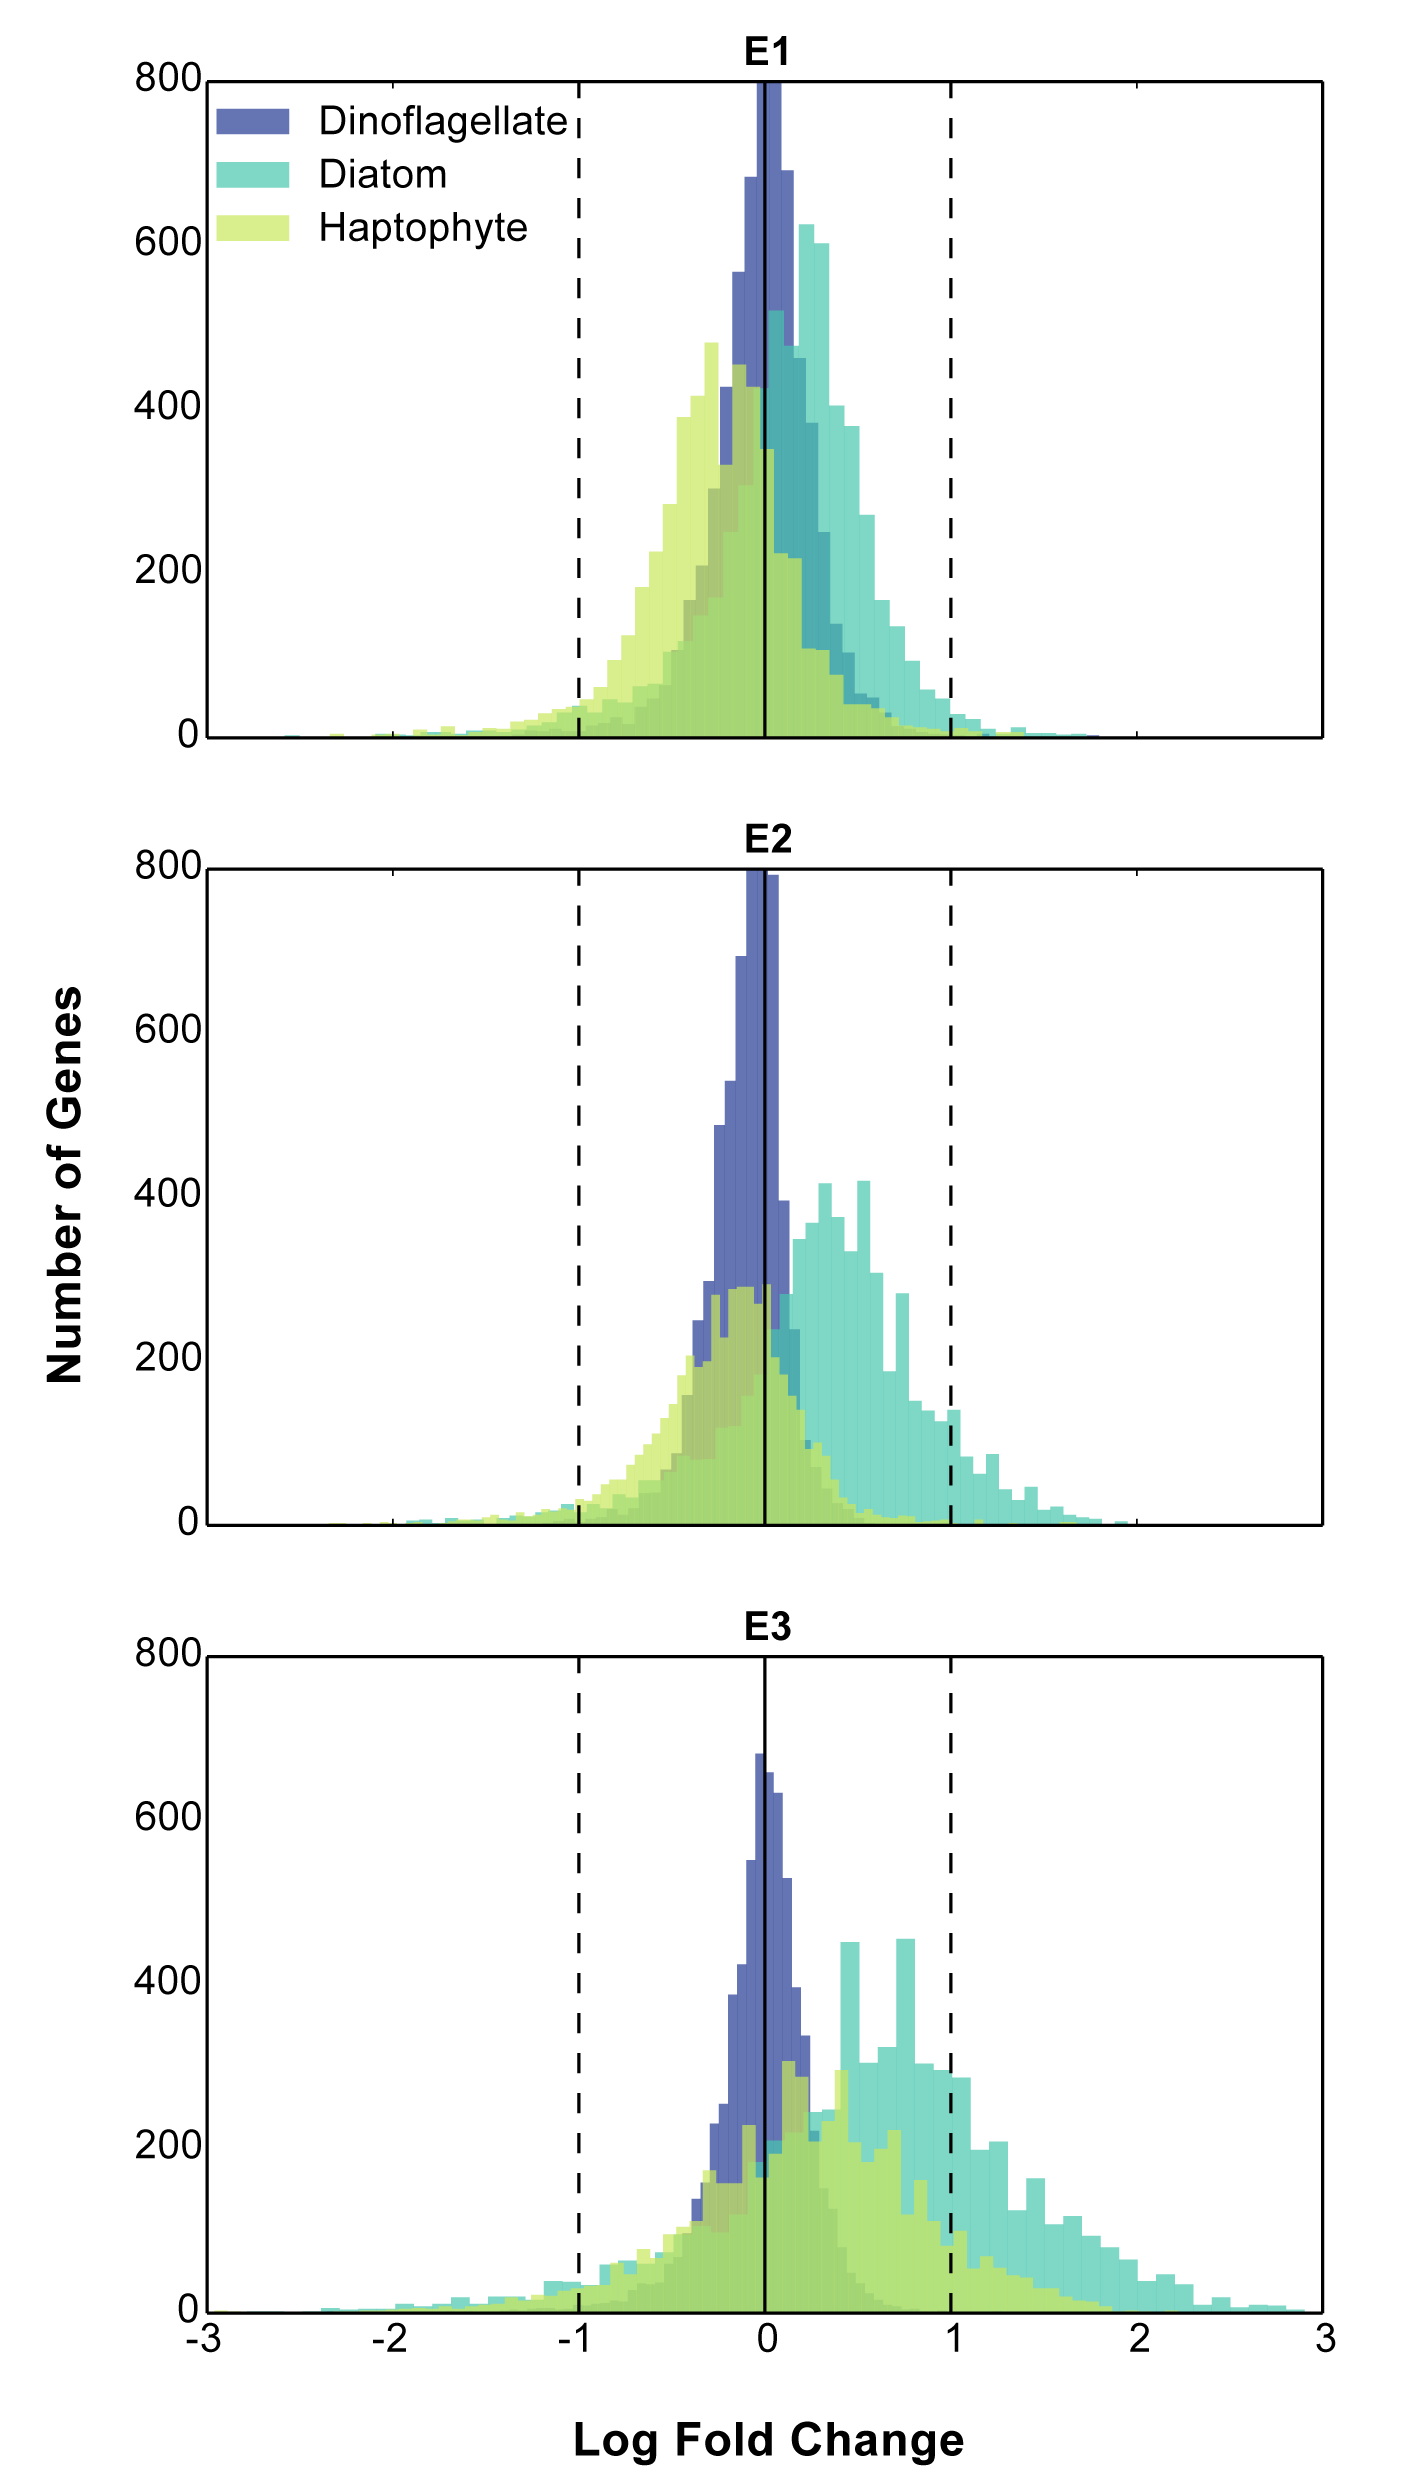
\includegraphics[width=.75\textwidth]{Images/C4_FigureS4.png}
    \caption[Distribution of log fold change following deep seawater (DSW) addition]{Distribution of log fold change following deep seawater (DSW) addition. Histogram of the number of genes falling within each of the log fold change bins for diatoms, haptophytes and dinoflagellates. Solid line indicates no fold change; dashed lines indicate 2 fold-change both up and down.}
  \label{fig:a4f4}
\end{figure}


%Supplemental Figure 5: Weight venn diagrams for up and down regulated genes

\begin{figure}[p!]
  \centering
    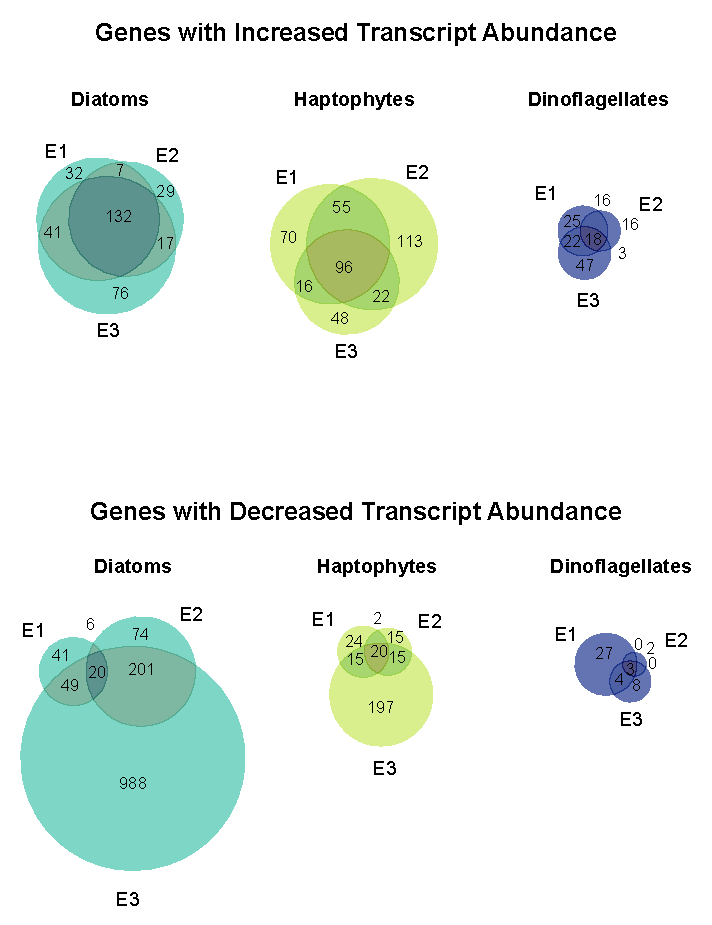
\includegraphics[width=1\textwidth]{Images/C4_FigureS5.pdf}
    \caption[Weighted Venn diagrams of genes with significantly different abundances following deep seawater (DSW) addition by functional group]{Weighted Venn diagrams of genes with significantly different abundances following deep seawater (DSW) addition by functional group. The uniqueness of KEGG orthologs with increased or decreased abundances as determined by ASC (2 fold-change, post-p > 0.95) across experiments was assessed for diatoms, haptophytes, and dinoflagellates.}
  \label{fig:a4f5}
\end{figure}


%Supplemental Figure 6: MANTA Plots

\begin{figure}[p!]
  \centering
    \includegraphics[width=.7\textwidth]{Images/C4_FigureS6.pdf}
    \caption[Microbial Assemblage Normalized Transcript Analysis (MANTA) ratio-averaged plots for global shifts in expression of KEGG orthologs]{Microbial Assemblage Normalized Transcript Analysis (MANTA) ratio-averaged plots for global shifts in expression of KEGG orthologs. Fold change ratio (R) and average read count (A) are plotted for read counts in the \emph{in situ} (S) and deep seawater (DSW) amendment (E) samples across the three sample pairs (S1:E1, S2:E2, S3:E3). The trimmed mean of fold-change values is noted as a gray solid line; orthologs unique to one library are separated by gray dashed lines. Pies indicate the taxonomic distribution of orthologous reads across the three functional groups. KEGG orthologs that were significantly differentially expressed (DE) (adjusted $P > 0.05$) are outlined in black and those not significantly DE are outlined in gray. DE KEGG orthologs that fall in the Energy Metabolism KEGG module are outlined in orange.}
  \label{fig:a4f6}
\end{figure}

%Supplemental Figure 7: QMF across incubation experiments

\begin{figure}[p!]
  \centering
    \includegraphics[width=1\textwidth]{Images/C4_FigureS7.pdf}
    \caption[Principal component analysis of the quantitative metabolic fingerprint (QMF) signals across \emph{in situ}, no addition control, and deep seawater amended samples]{Principal component analysis of the quantitative metabolic fingerprint (QMF) signals across \emph{in situ}, no addition control, and deep seawater (DSW) amended samples. Principal component analysis of the QMF signals for each of the functional groups across \emph{in situ} (S1-S3), control no addition (C1-C3) and DSW amendment (E1-E3); 95\% confidence ellipses are indicated for each of the sample types by functional group.}
  \label{fig:a4f7}
\end{figure}

\clearpage

\section{Supplemental Tables}

% Supplemental table with nutrient concentrations post treatment run for E and C
\begin{table}[h!]
\centering
\caption[Macronutrient concentrations in deep seawater ammendment and the incubation experiments after 168 hours]{Macronutrient concentrations in control no addition (C), DSW-amended incubations (E), and 700 m water used in DSW amendment incubations}
\label{tab:a4t1}
\newcolumntype{C}[1]{>{\centering\let\newline\\\arraybackslash\hspace{.5pt}}m{#1}}
\begin{tabular}{ccccc}

    
\hline
\multicolumn{1}{|c|}{\multirow{2}{*}{\textbf{Treatment}}} & \multicolumn{1}{c|}{\multirow{2}{*}{\textbf{\begin{tabular}[c]{@{}c@{}}Time post \\ inoculation (hours)\end{tabular}}}} & \multicolumn{1}{c|}{\multirow{2}{*}{\textbf{\begin{tabular}[c]{@{}c@{}}NO$_2^-$ + NO$_3^-$ \\ ($\mu M$)\end{tabular}}}} & \multicolumn{1}{c|}{\multirow{2}{*}{\textbf{\begin{tabular}[c]{@{}c@{}}PO$_4^{3-}$ \\ ($\mu M$)\end{tabular}}}} & \multicolumn{1}{c|}{\multirow{2}{*}{\textbf{\begin{tabular}[c]{@{}c@{}}SiO$_4^{4-}$\\ ($\mu M$)\end{tabular}}}} \\

\multicolumn{1}{|c|}{}                                    & \multicolumn{1}{c|}{}                                                        & \multicolumn{1}{c|}{}                                                                                    & \multicolumn{1}{c|}{}                                                                              & \multicolumn{1}{c|}{}                                                                            \\ \hline
\multicolumn{1}{|c|}{\textbf{C} (control no addition) *}  & \multicolumn{1}{c|}{168}                                                     & \multicolumn{1}{c|}{$0.12 \pm 0.03$}                                                                         & \multicolumn{1}{c|}{$0.12 \pm 0.02$}                                                                   & \multicolumn{1}{c|}{$1.91 \pm 0.2$}                                                                  \\ \hline
\multicolumn{1}{|c|}{\textbf{E} (+ 10\% DSW) *}           & \multicolumn{1}{c|}{168}                                                     & \multicolumn{1}{c|}{$1.9 \pm  .93$}                                                                          & \multicolumn{1}{c|}{$0.23 \pm 0.05$}                                                                   & \multicolumn{1}{c|}{$8.46 \pm 3.11$}                                                                 \\ \hline
\multicolumn{1}{|c|}{\textbf{DSW} (700 m water) *}        & \multicolumn{1}{c|}{N/A}                                                     & \multicolumn{1}{c|}{$37.5 \pm 1.68$}                                                                         & \multicolumn{1}{c|}{$3.14 \pm 0.03$}                                                                   & \multicolumn{1}{c|}{$83.4 \pm 9.33$}                                                                 \\ \hline
\multicolumn{5}{l}{\textit{* Nutrient data averaged for E1 and E2, nutrients were not assayed on E3.}}                                                                                                                                                                                                                                                                                                                                                     
\end{tabular}
\end{table}


\chapter{Chapter 4 Supplemental Information}
\label{sec:app4}
\raggedbottom

\clearpage

\section{Supplemental Figures}


\begin{figure}[htbp]
\centering
\includegraphics{images/A4_FigS1.pdf}
\caption[Regression of remotely-sensed SST
and model-based SST at a subset of swordfish conventional tag
locations]{Regression of MUR remotely-sensed SST
and HYCOM (model-based) SST at a subset of swordfish conventional tag
locations.}
\label{fig:a4f1}
\end{figure}

\begin{figure}[htbp]
\centering
\includegraphics[width=\textwidth]{images/A4_FigS2.pdf}
\caption[Drifter trajectories used as null movements in the eddy collocation analysis]{Drifter trajectories used as null movements (black lines) and bounding boxes (colored lines) for the focal regions in the eddy collocation analysis. The data presented here has been trimmed to one location per day to aid visualization. Regions designate the Gulf Stream (red), Sargasso Sea (green) and Gulf of Mexico (blue).}
\label{fig:a4f2}
\end{figure}

\begin{figure}[htbp]
\centering
\includegraphics[width=\textwidth]{images/A4_FigS3.pdf}
\caption[Generalized additive model diagnostics for swordfish catch-per-unit effort]{Diagnostic plots for the final model
from the generalized additive model analysis of catch-per-unit effort
data. Code for generating these plots in \texttt{R} is from \citet{Lam2014}.}
\label{fig:a4f3}
\end{figure}

\begin{figure}[htbp]
\centering
\includegraphics[width=\textwidth]{images/A4_FigS4.pdf}
\caption[Monthly latitude density distribution of
swordfish tagged with conventional tags]{Monthly density distribution of
swordfish tagged with conventional tags by latitude. Upper letters
indicate month and lower number labels indicate sample size of tagged
individuals.}
\label{fig:a4f4}
\end{figure}

\begin{figure}[htbp]
\centering
\includegraphics[height=8in, keepaspectratio]{images/A4_FigS5.pdf}
\caption[Distribution of SST and chlorophyll concentrations experienced by satellite and conventional-tagged swordfish in the North Atlantic]{Normalized density distributions of SST (A) and chlorophyll concentrations (B) experienced by satellite-tagged swordfish in the Azores (blue) and northwest Atlantic (red) and a subset of conventional-tagged swordfish in the North Atlantic (black) for which remote-sensing data was available.}
\label{fig:a4f5}
\end{figure}

\chapter{Chapter 5 Supplemental Information}
\label{sec:app5}
\raggedbottom

\clearpage

\section{Supplemental Figures}


\begin{figure}[htbp]
\centering
\includegraphics{images/A5_FigS1.pdf}
\caption[short]{long.}
\label{fig:a5f1}
\end{figure}


%% This defines the bibliography file (main.bib) and the bibliography style.
%% If you want to create a bibliography file by hand, change the contents of
%% this file to a `thebibliography' environment.  For more information 
%% see section 4.3 of the LaTeX manual.
\begin{singlespace}
\bibliography{main}
\bibliographystyle{myplainnat}
\end{singlespace}

\end{document}

